\documentclass{oci}
\usepackage[utf8]{inputenc}
\usepackage{lipsum}

% \usepackage{icpc_problem} % or wherever this package is stored
% \usepackage[spanish]{babel}
\usepackage[usenames,dvipsnames,svgnames,table]{xcolor}
\usepackage{amssymb}
\usepackage{float}
\usepackage{tikz}
\usepackage{color}
\usepackage{amsmath}
\usetikzlibrary{external}
\tikzexternalize[prefix=tikz/]
\usepackage{wrapfig}

\renewcommand{\u}{{\color{red}\texttt{+}}}
\renewcommand{\d}{{\color{blue}\texttt{-}}}

\def\NN{\mathbb{N}}
\def\ZZ{\mathbb{Z}}
\def\prob{\mathbb{P}}
\def\esp{\mathbb{E}}
\def\ag{\mathcal{A}}
\def\CC{\mathcal{C}}

\title{El camino del drag\'on}

\begin{document}
\maketitle
Nuestro héroe Olon-sonkú debe llegar al planeta de Jorgesama para aumentar su poder.
Si supiera la posición del planeta podría usar la teletransportación. Lamentablemente Olon-sokú no sabe exactamente dónde está el planeta y sólo sabe que este se encuentra en algún punto siguiendo el \emph{camino del dragón}, un camino infinito de intrincada estructura. 
% Olon-sokú no sabe exactamente dónde está el planeta y sólo sabe que 
%este se encuentra en algún punto del \emph{camino del dragón}, un camino infinito de intrincada estructura. 
Por fortuna %para Olon-sokú, que si bien tiene gran fuerza su inteligencia es bastante escasa ****, 
su astuta amiga Bulnelman lleva años estudiando este camino, y ha descubierto que puede ser recorrido de manera simple mediante \emph{secuencias del dragón} que son movimientos que se deben seguir para avanzar por el camino infinito.

Para describir una \emph{secuencia del dragón} denotaremos con una ``$A$'' la acción de avanzar un paso, con una ``$R$'' la acción de rotar $90^{\circ}$ grados a la derecha y con una ``$L$'' la acción de rotar $90^{\circ}$ a la izquierda.
Describiremos las secuencias del dragón usando secuencias de estas letras. No obstante, no cualquier secuencia corresponde a una secuencia del dragón válida.
Las secuencias válidas son generadas por un sistema de \emph{reemplazos} que usa dos símbolos especiales, ``$\u$'' y ``$\d$'', y que siguen las siguientes reglas.
Un ``$\u$'' se debe reemplazar por la secuencia ``$\u\ R\ \d\ A\ R$'' y un ``$\d$'' se debe reemplazar por la secuencia ``$L\ A\ \u\ L\ \d$'', lo que se muestra en el siguiente esquema.
\begin{center}
\scalebox{0.8}
{ 
\input{reglas.pspdftex}}
\end{center}

Para generar secuencias del dragón hay que comenzar con la secuencia ``$A\ \u$'' y aplicar iterativamente las reglas de reemplazo.
A continuación se muestra un esquema con la aplicación de las reglas en tres iteraciones consecutivas iniciando en la secuencia ``$A\ \u$''.
\begin{center}
\scalebox{0.8}
{ 
\input{aplicacion.pspdftex}}
\end{center}

Comenzando con ``$A\ \u$'', en el primer paso el símbolo ``$\u$'' es reemplazado por ``$\u\ R\ \d\ A\ R$'' resultando la secuencia ``$A\ \u\ R\ \d\ A\ R$'' que se ve en el nivel 1 en el diagrama.
A continuación en esa secuencia se reemplazan ``$\u$'' por ``$\u\ R\ \d\ A\ R$'' y ``$\d$'' por ``$L\ A\ \u\ L\ \d$'' dando como resultado la secuencia 
``$A\ \u\ R\ \d\ A\ R\ R\ L\ A\ \u\ L\ \d\ A\ R$'' en el nivel 2 del diagrama.
Después de la tercera iteración se obtiene la secuencia que se ve en el nivel 3 del diagrama y que corresponde a
$$\text{``}A\ \u\ R\ \d\ A\ R\ R\ L\ A\ \u\ L\ \d\ A\ R\ R\ L\ A\ \u\ R\ \d\ A\ R\ L\ L\ A\ \u\ L\ \d\ A\ R\text{''}.$$

Para generar finalmente las secuencias del dragón, debemos simplemente eliminar los ``$\u$'' y ``$\d$'' de las secuencias generadas en el anterior proceso.
El siguiente diagrama muestra las secuencias del dragón generadas a partir de las primeras tres iteraciones.
\begin{center}
\scalebox{0.8}
{ 
\input{caminos.pspdftex}}
\end{center}

Notar que después de cada iteración la secuencia resultante es una extensión de la anterior.
Esto significa que después de cada iteración nos acercamos más al camino del dragón real. Como lo notó Bulnelman, si siguiéramos con el proceso hasta el infinito obtendríamos una secuencia que define la forma de avanzar por el camino del dragón completo.

Bulnelman tiene el problema de Olon-soukú casi resuelto, pues sus investigaciones le han permitido determinar que el planeta de Jorgesama se encuentra avanzando exactamente $N$ pasos en el camino del dragón. Lo único que necesitamos ahora es saber dónde quedaría exactamente una persona que avanzara $N$ pasos del camino, y es aquí donde tu ayuda se hace imprescindible.

%Cada una de las secuencias del dragón corresponde a una serie de acciones que hay que hacer para recorrer el camino correspondiente.
%Para determinar la posición en que queda Olon-sonkú después de realizar las acciones supondremos que siempre comienza en la posición $(0,0)$ mirando hacia el norte.

Supondremos que para recorrer el camino del dragón se comienza siempre en la posición $(0,0)$ mirando hacia el norte.
A continuación se muestra un ejemplo donde se ejecutan las acciones para la secuencia ``$A\ R\ A\ R\ R\ L\ A\ L\ A\ R\ R\ L\ A\ R\ A\ R\ L\ L\ A\ L\ A\ R$'' junto a una figura de ilustración:
% \newpage
\\

\begin{minipage}{0.45\textwidth}
\begin{itemize}
	{\footnotesize \item Comenzamos en $(0,0)$ mirando al norte
	\item $A$:  Avanzar, llega a $(0,1)$ mirando todavía hacia el norte.
	\item $R\ A$: Rotar a la derecha y avanzar, llega a $(1,1)$ y mirando hacia el este.
	\item $R\ R\ L\ A$: Rotar dos veces a la derecha, una vez a la izquierda y luego avanzar, llega a $(1,0)$ y mirando hacia sur.
	\item $L\ A$: Llega a $(2,0)$ mirando hacia el este.
	\item $R\ R\ L\ A$: Llega a $(2,-1)$ mirando hacia el sur.
	\item $R\ A$: Llega a $(1,-1)$ mirando hacia el oeste.
	\item $R\ L\ L\ A$: Llega a $(1,-2)$ mirando hacia el sur.
	\item $L\ A\ R$:  Termina en $(2,-2)$ mirando hacia el sur.}
\end{itemize}
\end{minipage}
~%
\begin{minipage}{0.5\textwidth}
\begin{center}
		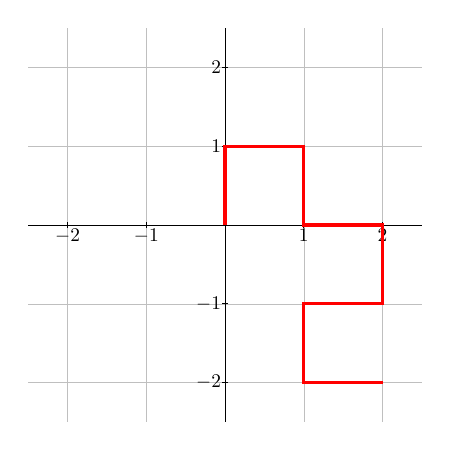
\begin{tikzpicture}
	% \begin{scope}[scale = 0.6, shift={(-15,0)},rotate=0]
	% \draw[thick,red] (0,0) --(0,1);
	% \draw[fill = black] (0,0) circle (0.1);
	% \end{scope}
	% \begin{scope}[scale = 0.6, shift={(-12,0)},rotate=0]
	% \draw[thick,red] (0,0) --(0,1) --(1,1);
	% \draw[fill = black] (0,0) circle (0.1);
	% \end{scope}
	% \begin{scope}[scale = 0.6, shift={(-9,0)},rotate=0]
	% \draw[thick,red] (0,0) --(0,1) --(1,1) --(1,0);
	% \draw[fill = black] (0,0) circle (0.1);
	% \end{scope}
	% \begin{scope}[scale = 0.6, shift={(-6,0)},rotate=0]
	% \draw[thick,red] (0,0) --(0,1) --(1,1) --(1,0) -- (2,0);
	% \draw[fill = black] (0,0) circle (0.1);
	% \end{scope}
	% \begin{scope}[scale = 0.6, shift={(-3,0)},rotate=0]
	% \draw[thick,red] (0,0) --(0,1) --(1,1) --(1,0) -- (2,0) --(2,-1);
	% \draw[fill = black] (0,0) circle (0.1);
	% \end{scope}
	% \begin{scope}[scale = 0.6, shift={(0,0)},rotate=0]
	% \draw[thick,red] (0,0) --(0,1) --(1,1) --(1,0) -- (2,0) --(2,-1) -- (1,-1);
	% \draw[fill = black] (0,0) circle (0.1);
	% \end{scope}
	% \begin{scope}[scale = 0.6, shift={(3,0)},rotate=0]
	% \draw[thick,red] (0,0) --(0,1) --(1,1) --(1,0) -- (2,0) --(2,-1) -- (1,-1)--(1,-2);
	% \draw[fill = black] (0,0) circle (0.1);
	% \end{scope}
	% \begin{scope}[scale = 1, shift={(0,0)},rotate=0]
    \draw[step=1, lightgray, very thin] (2.5,2.5) grid (-2.5,-2.5);
    \foreach \i in {-2,-1,1,2}
       \draw (\i, -1pt) -- (\i, 1pt) node[anchor=north, scale=0.7]{$\i$};
    \foreach \i in {-2,-1,1,2}
       \draw (-1pt,\i) -- (1pt,\i) node[anchor=east, scale=0.7]{$\i$};
  \draw[thin] (0,-2.5) -- (0,2.5);
  \draw[thin] (-2.5,0) -- (2.5, 0);
	\draw[very thick,red] (0,0) --(0,1) --(1,1) --(1,0) -- (2,0) --(2,-1) -- (1,-1)--(1,-2) -- (2,-2);
	% \draw[fill = black] (0,0) circle (0.1);
	%\end{scope}
	\end{tikzpicture}
\end{center}
\end{minipage}
\\

Nota que en el recorrido anteriormente descrito se avanzaron $N=8$ pasos. Esencialmente para una secuencia del dragón, la cantidad de pasos que se avanza equivale a la cantidad de veces que la letra ``$A$'' aparece en la secuencia.
Nota además que para seguir $N$ pasos del camino del dragón, se debe considerar una secuencia con al menos $N$ letras ``$A$''. 
Por ejemplo, para avanzar $5$ pasos, hay que considerar la secuencia ``$A\ R\ A\ R\ R\ L\ A\ L\ A\ R\ R\ L\ A\ R\ A\ R\ L\ L\ A\ L\ A\ R$'' y ejecutar
las primeras 5 acciones avanzar, lo que nos dejaría en la posición $(2,-1)$.
Si tienes curiosidad acerca de la forma del mítico camino del dragón, en la figura de la siguiente página se muestra una porción más grande del camino, una en donde se han avanzado $2^{12}-1=$\ 4.095 pasos.
%Esto dejaría a Olon-sonkú en la posición $(2,-1)$.

%Diremos que un recorrido del dragón tiene largo $N$ si se ejecuta la acción avanzar $N$ veces.
%Por ejemplo, el recorrido descrito anteriormente tiene largo $N = 8$.
%Notar que para hacer un recorrido de largo $N$ hay que considerar una secuencia del dragón que tenga al menos $N$ acciones avanzar.
%Por ejemplo si se quiere hacer un recorrido de largo $N=5$ hay que considerar la secuencia $ARARRLALARRLARARLLALAR$ y ejecutar
%las primeras 5 acciones avanzar.
%Esto dejaría a Olon-sonkú en la posición $(2,-1)$.

Olon-sokú ya no puede esperar para teletrasportarse done Jorgesama, sólo necesita las coordenadas. Por su parte Bulnelman ya sabe la cantidad de pasos que habría que avanzar en el camino del dragón para llegar al planeta. Ahora sólo falta tu parte.
%Supón que Bulnelman sabe que el planeta de Jorgesama se encuentra al final del recorrido del dragón de largo $N$.
%?`Puedes ayudarnos a saber cual es la posición exacta del planeta del gran Jorgesama?


\begin{inputDescription}
La entrada consiste en una línea con un único entero positivo $N$, que corresponde a la cantidad de pasos que hay que avanzar en el camino del dragón para llegar al planeta de Jorgesama.
%Tu programa debe calcular las coordenadas del final del recorrido del dragón de largo $N$.
\end{inputDescription}

\begin{outputDescription}
Debes imprimir una única línea con dos enteros $x$ e $y$ separados por un espacio.
Estos enteros corresponden a las coordenadas del planeta del gran Jorgesama.
\end{outputDescription}

\begin{scoreDescription}
\score{10} Se probarán varios casos donde $1 \leq N \leq 8$.
\score{20} Se probarán varios casos donde $1 \leq N \leq 100$.
\score{40} Se probarán varios casos donde $1 \leq N \leq 10^5$.
\score{30} Se probarán varios casos donde $1 \leq N \leq 10^{15}$. 
\\
\\
{\bf Nota:} en la última subtarea el entero $N$ debe ser leído en una variable de tipo long long.
\end{scoreDescription}

\begin{sampleDescription}
\sampleIO{sample1}
\sampleIO{sample2}
\sampleIO{sample3}
\sampleIO{sample4}
\sampleIO{sample5}
\sampleIO{sample6}
\end{sampleDescription}


%\begin{wrapfigure}{r}{0.9\textwidth}
 \begin{figure*}[h!]
%  \centering
	 \begin{center}
			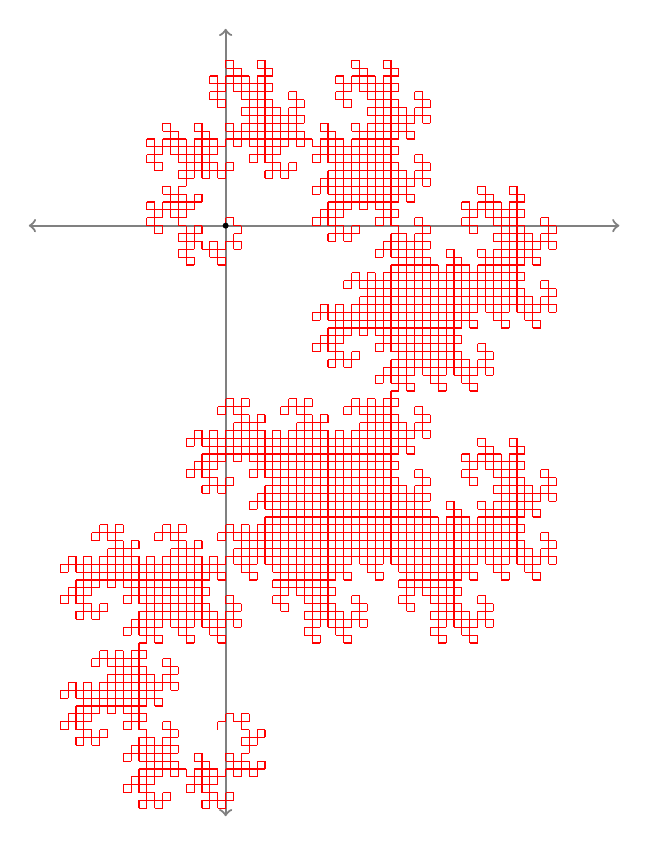
\begin{tikzpicture}[remember picture,scale = 0.1]
\draw[thick, black!50, <->] (-25,0) to (50,0);
\draw[thick, black!50, <->] (0,-75) to (0,25);
\draw[,-,red] (0,0) to (0,1);
\draw[,-,red] (0,1) to (1,1);
\draw[,-,red] (1,1) to (1,0);
\draw[,-,red] (1,0) to (2,0);
\draw[,-,red] (2,0) to (2,-1);
\draw[,-,red] (2,-1) to (1,-1);
\draw[,-,red] (1,-1) to (1,-2);
\draw[,-,red] (1,-2) to (2,-2);
\draw[,-,red] (2,-2) to (2,-3);
\draw[,-,red] (2,-3) to (1,-3);
\draw[,-,red] (1,-3) to (1,-2);
\draw[,-,red] (1,-2) to (0,-2);
\draw[,-,red] (0,-2) to (0,-3);
\draw[,-,red] (0,-3) to (-1,-3);
\draw[,-,red] (-1,-3) to (-1,-4);
\draw[,-,red] (-1,-4) to (0,-4);
\draw[,-,red] (0,-4) to (0,-5);
\draw[,-,red] (0,-5) to (-1,-5);
\draw[,-,red] (-1,-5) to (-1,-4);
\draw[,-,red] (-1,-4) to (-2,-4);
\draw[,-,red] (-2,-4) to (-2,-3);
\draw[,-,red] (-2,-3) to (-1,-3);
\draw[,-,red] (-1,-3) to (-1,-2);
\draw[,-,red] (-1,-2) to (-2,-2);
\draw[,-,red] (-2,-2) to (-2,-3);
\draw[,-,red] (-2,-3) to (-3,-3);
\draw[,-,red] (-3,-3) to (-3,-2);
\draw[,-,red] (-3,-2) to (-4,-2);
\draw[,-,red] (-4,-2) to (-4,-3);
\draw[,-,red] (-4,-3) to (-5,-3);
\draw[,-,red] (-5,-3) to (-5,-4);
\draw[,-,red] (-5,-4) to (-4,-4);
\draw[,-,red] (-4,-4) to (-4,-5);
\draw[,-,red] (-4,-5) to (-5,-5);
\draw[,-,red] (-5,-5) to (-5,-4);
\draw[,-,red] (-5,-4) to (-6,-4);
\draw[,-,red] (-6,-4) to (-6,-3);
\draw[,-,red] (-6,-3) to (-5,-3);
\draw[,-,red] (-5,-3) to (-5,-2);
\draw[,-,red] (-5,-2) to (-6,-2);
\draw[,-,red] (-6,-2) to (-6,-1);
\draw[,-,red] (-6,-1) to (-5,-1);
\draw[,-,red] (-5,-1) to (-5,-2);
\draw[,-,red] (-5,-2) to (-4,-2);
\draw[,-,red] (-4,-2) to (-4,-1);
\draw[,-,red] (-4,-1) to (-3,-1);
\draw[,-,red] (-3,-1) to (-3,0);
\draw[,-,red] (-3,0) to (-4,0);
\draw[,-,red] (-4,0) to (-4,-1);
\draw[,-,red] (-4,-1) to (-5,-1);
\draw[,-,red] (-5,-1) to (-5,0);
\draw[,-,red] (-5,0) to (-6,0);
\draw[,-,red] (-6,0) to (-6,1);
\draw[,-,red] (-6,1) to (-5,1);
\draw[,-,red] (-5,1) to (-5,2);
\draw[,-,red] (-5,2) to (-6,2);
\draw[,-,red] (-6,2) to (-6,1);
\draw[,-,red] (-6,1) to (-7,1);
\draw[,-,red] (-7,1) to (-7,2);
\draw[,-,red] (-7,2) to (-8,2);
\draw[,-,red] (-8,2) to (-8,1);
\draw[,-,red] (-8,1) to (-9,1);
\draw[,-,red] (-9,1) to (-9,0);
\draw[,-,red] (-9,0) to (-8,0);
\draw[,-,red] (-8,0) to (-8,-1);
\draw[,-,red] (-8,-1) to (-9,-1);
\draw[,-,red] (-9,-1) to (-9,0);
\draw[,-,red] (-9,0) to (-10,0);
\draw[,-,red] (-10,0) to (-10,1);
\draw[,-,red] (-10,1) to (-9,1);
\draw[,-,red] (-9,1) to (-9,2);
\draw[,-,red] (-9,2) to (-10,2);
\draw[,-,red] (-10,2) to (-10,3);
\draw[,-,red] (-10,3) to (-9,3);
\draw[,-,red] (-9,3) to (-9,2);
\draw[,-,red] (-9,2) to (-8,2);
\draw[,-,red] (-8,2) to (-8,3);
\draw[,-,red] (-8,3) to (-7,3);
\draw[,-,red] (-7,3) to (-7,4);
\draw[,-,red] (-7,4) to (-8,4);
\draw[,-,red] (-8,4) to (-8,5);
\draw[,-,red] (-8,5) to (-7,5);
\draw[,-,red] (-7,5) to (-7,4);
\draw[,-,red] (-7,4) to (-6,4);
\draw[,-,red] (-6,4) to (-6,3);
\draw[,-,red] (-6,3) to (-7,3);
\draw[,-,red] (-7,3) to (-7,2);
\draw[,-,red] (-7,2) to (-6,2);
\draw[,-,red] (-6,2) to (-6,3);
\draw[,-,red] (-6,3) to (-5,3);
\draw[,-,red] (-5,3) to (-5,2);
\draw[,-,red] (-5,2) to (-4,2);
\draw[,-,red] (-4,2) to (-4,3);
\draw[,-,red] (-4,3) to (-3,3);
\draw[,-,red] (-3,3) to (-3,4);
\draw[,-,red] (-3,4) to (-4,4);
\draw[,-,red] (-4,4) to (-4,3);
\draw[,-,red] (-4,3) to (-5,3);
\draw[,-,red] (-5,3) to (-5,4);
\draw[,-,red] (-5,4) to (-6,4);
\draw[,-,red] (-6,4) to (-6,5);
\draw[,-,red] (-6,5) to (-5,5);
\draw[,-,red] (-5,5) to (-5,6);
\draw[,-,red] (-5,6) to (-6,6);
\draw[,-,red] (-6,6) to (-6,7);
\draw[,-,red] (-6,7) to (-5,7);
\draw[,-,red] (-5,7) to (-5,6);
\draw[,-,red] (-5,6) to (-4,6);
\draw[,-,red] (-4,6) to (-4,7);
\draw[,-,red] (-4,7) to (-3,7);
\draw[,-,red] (-3,7) to (-3,8);
\draw[,-,red] (-3,8) to (-4,8);
\draw[,-,red] (-4,8) to (-4,7);
\draw[,-,red] (-4,7) to (-5,7);
\draw[,-,red] (-5,7) to (-5,8);
\draw[,-,red] (-5,8) to (-6,8);
\draw[,-,red] (-6,8) to (-6,9);
\draw[,-,red] (-6,9) to (-5,9);
\draw[,-,red] (-5,9) to (-5,10);
\draw[,-,red] (-5,10) to (-6,10);
\draw[,-,red] (-6,10) to (-6,9);
\draw[,-,red] (-6,9) to (-7,9);
\draw[,-,red] (-7,9) to (-7,10);
\draw[,-,red] (-7,10) to (-8,10);
\draw[,-,red] (-8,10) to (-8,9);
\draw[,-,red] (-8,9) to (-9,9);
\draw[,-,red] (-9,9) to (-9,8);
\draw[,-,red] (-9,8) to (-8,8);
\draw[,-,red] (-8,8) to (-8,7);
\draw[,-,red] (-8,7) to (-9,7);
\draw[,-,red] (-9,7) to (-9,8);
\draw[,-,red] (-9,8) to (-10,8);
\draw[,-,red] (-10,8) to (-10,9);
\draw[,-,red] (-10,9) to (-9,9);
\draw[,-,red] (-9,9) to (-9,10);
\draw[,-,red] (-9,10) to (-10,10);
\draw[,-,red] (-10,10) to (-10,11);
\draw[,-,red] (-10,11) to (-9,11);
\draw[,-,red] (-9,11) to (-9,10);
\draw[,-,red] (-9,10) to (-8,10);
\draw[,-,red] (-8,10) to (-8,11);
\draw[,-,red] (-8,11) to (-7,11);
\draw[,-,red] (-7,11) to (-7,12);
\draw[,-,red] (-7,12) to (-8,12);
\draw[,-,red] (-8,12) to (-8,13);
\draw[,-,red] (-8,13) to (-7,13);
\draw[,-,red] (-7,13) to (-7,12);
\draw[,-,red] (-7,12) to (-6,12);
\draw[,-,red] (-6,12) to (-6,11);
\draw[,-,red] (-6,11) to (-7,11);
\draw[,-,red] (-7,11) to (-7,10);
\draw[,-,red] (-7,10) to (-6,10);
\draw[,-,red] (-6,10) to (-6,11);
\draw[,-,red] (-6,11) to (-5,11);
\draw[,-,red] (-5,11) to (-5,10);
\draw[,-,red] (-5,10) to (-4,10);
\draw[,-,red] (-4,10) to (-4,11);
\draw[,-,red] (-4,11) to (-3,11);
\draw[,-,red] (-3,11) to (-3,12);
\draw[,-,red] (-3,12) to (-4,12);
\draw[,-,red] (-4,12) to (-4,13);
\draw[,-,red] (-4,13) to (-3,13);
\draw[,-,red] (-3,13) to (-3,12);
\draw[,-,red] (-3,12) to (-2,12);
\draw[,-,red] (-2,12) to (-2,11);
\draw[,-,red] (-2,11) to (-3,11);
\draw[,-,red] (-3,11) to (-3,10);
\draw[,-,red] (-3,10) to (-2,10);
\draw[,-,red] (-2,10) to (-2,9);
\draw[,-,red] (-2,9) to (-3,9);
\draw[,-,red] (-3,9) to (-3,10);
\draw[,-,red] (-3,10) to (-4,10);
\draw[,-,red] (-4,10) to (-4,9);
\draw[,-,red] (-4,9) to (-5,9);
\draw[,-,red] (-5,9) to (-5,8);
\draw[,-,red] (-5,8) to (-4,8);
\draw[,-,red] (-4,8) to (-4,9);
\draw[,-,red] (-4,9) to (-3,9);
\draw[,-,red] (-3,9) to (-3,8);
\draw[,-,red] (-3,8) to (-2,8);
\draw[,-,red] (-2,8) to (-2,7);
\draw[,-,red] (-2,7) to (-3,7);
\draw[,-,red] (-3,7) to (-3,6);
\draw[,-,red] (-3,6) to (-2,6);
\draw[,-,red] (-2,6) to (-2,7);
\draw[,-,red] (-2,7) to (-1,7);
\draw[,-,red] (-1,7) to (-1,6);
\draw[,-,red] (-1,6) to (0,6);
\draw[,-,red] (0,6) to (0,7);
\draw[,-,red] (0,7) to (1,7);
\draw[,-,red] (1,7) to (1,8);
\draw[,-,red] (1,8) to (0,8);
\draw[,-,red] (0,8) to (0,7);
\draw[,-,red] (0,7) to (-1,7);
\draw[,-,red] (-1,7) to (-1,8);
\draw[,-,red] (-1,8) to (-2,8);
\draw[,-,red] (-2,8) to (-2,9);
\draw[,-,red] (-2,9) to (-1,9);
\draw[,-,red] (-1,9) to (-1,10);
\draw[,-,red] (-1,10) to (-2,10);
\draw[,-,red] (-2,10) to (-2,11);
\draw[,-,red] (-2,11) to (-1,11);
\draw[,-,red] (-1,11) to (-1,10);
\draw[,-,red] (-1,10) to (0,10);
\draw[,-,red] (0,10) to (0,11);
\draw[,-,red] (0,11) to (1,11);
\draw[,-,red] (1,11) to (1,12);
\draw[,-,red] (1,12) to (0,12);
\draw[,-,red] (0,12) to (0,13);
\draw[,-,red] (0,13) to (1,13);
\draw[,-,red] (1,13) to (1,12);
\draw[,-,red] (1,12) to (2,12);
\draw[,-,red] (2,12) to (2,11);
\draw[,-,red] (2,11) to (1,11);
\draw[,-,red] (1,11) to (1,10);
\draw[,-,red] (1,10) to (2,10);
\draw[,-,red] (2,10) to (2,11);
\draw[,-,red] (2,11) to (3,11);
\draw[,-,red] (3,11) to (3,10);
\draw[,-,red] (3,10) to (4,10);
\draw[,-,red] (4,10) to (4,11);
\draw[,-,red] (4,11) to (5,11);
\draw[,-,red] (5,11) to (5,12);
\draw[,-,red] (5,12) to (4,12);
\draw[,-,red] (4,12) to (4,11);
\draw[,-,red] (4,11) to (3,11);
\draw[,-,red] (3,11) to (3,12);
\draw[,-,red] (3,12) to (2,12);
\draw[,-,red] (2,12) to (2,13);
\draw[,-,red] (2,13) to (3,13);
\draw[,-,red] (3,13) to (3,14);
\draw[,-,red] (3,14) to (2,14);
\draw[,-,red] (2,14) to (2,15);
\draw[,-,red] (2,15) to (3,15);
\draw[,-,red] (3,15) to (3,14);
\draw[,-,red] (3,14) to (4,14);
\draw[,-,red] (4,14) to (4,15);
\draw[,-,red] (4,15) to (5,15);
\draw[,-,red] (5,15) to (5,16);
\draw[,-,red] (5,16) to (4,16);
\draw[,-,red] (4,16) to (4,15);
\draw[,-,red] (4,15) to (3,15);
\draw[,-,red] (3,15) to (3,16);
\draw[,-,red] (3,16) to (2,16);
\draw[,-,red] (2,16) to (2,17);
\draw[,-,red] (2,17) to (3,17);
\draw[,-,red] (3,17) to (3,18);
\draw[,-,red] (3,18) to (2,18);
\draw[,-,red] (2,18) to (2,17);
\draw[,-,red] (2,17) to (1,17);
\draw[,-,red] (1,17) to (1,18);
\draw[,-,red] (1,18) to (0,18);
\draw[,-,red] (0,18) to (0,17);
\draw[,-,red] (0,17) to (-1,17);
\draw[,-,red] (-1,17) to (-1,16);
\draw[,-,red] (-1,16) to (0,16);
\draw[,-,red] (0,16) to (0,15);
\draw[,-,red] (0,15) to (-1,15);
\draw[,-,red] (-1,15) to (-1,16);
\draw[,-,red] (-1,16) to (-2,16);
\draw[,-,red] (-2,16) to (-2,17);
\draw[,-,red] (-2,17) to (-1,17);
\draw[,-,red] (-1,17) to (-1,18);
\draw[,-,red] (-1,18) to (-2,18);
\draw[,-,red] (-2,18) to (-2,19);
\draw[,-,red] (-2,19) to (-1,19);
\draw[,-,red] (-1,19) to (-1,18);
\draw[,-,red] (-1,18) to (0,18);
\draw[,-,red] (0,18) to (0,19);
\draw[,-,red] (0,19) to (1,19);
\draw[,-,red] (1,19) to (1,20);
\draw[,-,red] (1,20) to (0,20);
\draw[,-,red] (0,20) to (0,21);
\draw[,-,red] (0,21) to (1,21);
\draw[,-,red] (1,21) to (1,20);
\draw[,-,red] (1,20) to (2,20);
\draw[,-,red] (2,20) to (2,19);
\draw[,-,red] (2,19) to (1,19);
\draw[,-,red] (1,19) to (1,18);
\draw[,-,red] (1,18) to (2,18);
\draw[,-,red] (2,18) to (2,19);
\draw[,-,red] (2,19) to (3,19);
\draw[,-,red] (3,19) to (3,18);
\draw[,-,red] (3,18) to (4,18);
\draw[,-,red] (4,18) to (4,19);
\draw[,-,red] (4,19) to (5,19);
\draw[,-,red] (5,19) to (5,20);
\draw[,-,red] (5,20) to (4,20);
\draw[,-,red] (4,20) to (4,21);
\draw[,-,red] (4,21) to (5,21);
\draw[,-,red] (5,21) to (5,20);
\draw[,-,red] (5,20) to (6,20);
\draw[,-,red] (6,20) to (6,19);
\draw[,-,red] (6,19) to (5,19);
\draw[,-,red] (5,19) to (5,18);
\draw[,-,red] (5,18) to (6,18);
\draw[,-,red] (6,18) to (6,17);
\draw[,-,red] (6,17) to (5,17);
\draw[,-,red] (5,17) to (5,18);
\draw[,-,red] (5,18) to (4,18);
\draw[,-,red] (4,18) to (4,17);
\draw[,-,red] (4,17) to (3,17);
\draw[,-,red] (3,17) to (3,16);
\draw[,-,red] (3,16) to (4,16);
\draw[,-,red] (4,16) to (4,17);
\draw[,-,red] (4,17) to (5,17);
\draw[,-,red] (5,17) to (5,16);
\draw[,-,red] (5,16) to (6,16);
\draw[,-,red] (6,16) to (6,15);
\draw[,-,red] (6,15) to (5,15);
\draw[,-,red] (5,15) to (5,14);
\draw[,-,red] (5,14) to (6,14);
\draw[,-,red] (6,14) to (6,15);
\draw[,-,red] (6,15) to (7,15);
\draw[,-,red] (7,15) to (7,14);
\draw[,-,red] (7,14) to (8,14);
\draw[,-,red] (8,14) to (8,15);
\draw[,-,red] (8,15) to (9,15);
\draw[,-,red] (9,15) to (9,16);
\draw[,-,red] (9,16) to (8,16);
\draw[,-,red] (8,16) to (8,17);
\draw[,-,red] (8,17) to (9,17);
\draw[,-,red] (9,17) to (9,16);
\draw[,-,red] (9,16) to (10,16);
\draw[,-,red] (10,16) to (10,15);
\draw[,-,red] (10,15) to (9,15);
\draw[,-,red] (9,15) to (9,14);
\draw[,-,red] (9,14) to (10,14);
\draw[,-,red] (10,14) to (10,13);
\draw[,-,red] (10,13) to (9,13);
\draw[,-,red] (9,13) to (9,14);
\draw[,-,red] (9,14) to (8,14);
\draw[,-,red] (8,14) to (8,13);
\draw[,-,red] (8,13) to (7,13);
\draw[,-,red] (7,13) to (7,12);
\draw[,-,red] (7,12) to (8,12);
\draw[,-,red] (8,12) to (8,11);
\draw[,-,red] (8,11) to (7,11);
\draw[,-,red] (7,11) to (7,12);
\draw[,-,red] (7,12) to (6,12);
\draw[,-,red] (6,12) to (6,13);
\draw[,-,red] (6,13) to (7,13);
\draw[,-,red] (7,13) to (7,14);
\draw[,-,red] (7,14) to (6,14);
\draw[,-,red] (6,14) to (6,13);
\draw[,-,red] (6,13) to (5,13);
\draw[,-,red] (5,13) to (5,14);
\draw[,-,red] (5,14) to (4,14);
\draw[,-,red] (4,14) to (4,13);
\draw[,-,red] (4,13) to (3,13);
\draw[,-,red] (3,13) to (3,12);
\draw[,-,red] (3,12) to (4,12);
\draw[,-,red] (4,12) to (4,13);
\draw[,-,red] (4,13) to (5,13);
\draw[,-,red] (5,13) to (5,12);
\draw[,-,red] (5,12) to (6,12);
\draw[,-,red] (6,12) to (6,11);
\draw[,-,red] (6,11) to (5,11);
\draw[,-,red] (5,11) to (5,10);
\draw[,-,red] (5,10) to (6,10);
\draw[,-,red] (6,10) to (6,9);
\draw[,-,red] (6,9) to (5,9);
\draw[,-,red] (5,9) to (5,10);
\draw[,-,red] (5,10) to (4,10);
\draw[,-,red] (4,10) to (4,9);
\draw[,-,red] (4,9) to (3,9);
\draw[,-,red] (3,9) to (3,8);
\draw[,-,red] (3,8) to (4,8);
\draw[,-,red] (4,8) to (4,9);
\draw[,-,red] (4,9) to (5,9);
\draw[,-,red] (5,9) to (5,8);
\draw[,-,red] (5,8) to (6,8);
\draw[,-,red] (6,8) to (6,7);
\draw[,-,red] (6,7) to (5,7);
\draw[,-,red] (5,7) to (5,6);
\draw[,-,red] (5,6) to (6,6);
\draw[,-,red] (6,6) to (6,7);
\draw[,-,red] (6,7) to (7,7);
\draw[,-,red] (7,7) to (7,6);
\draw[,-,red] (7,6) to (8,6);
\draw[,-,red] (8,6) to (8,7);
\draw[,-,red] (8,7) to (9,7);
\draw[,-,red] (9,7) to (9,8);
\draw[,-,red] (9,8) to (8,8);
\draw[,-,red] (8,8) to (8,7);
\draw[,-,red] (8,7) to (7,7);
\draw[,-,red] (7,7) to (7,8);
\draw[,-,red] (7,8) to (6,8);
\draw[,-,red] (6,8) to (6,9);
\draw[,-,red] (6,9) to (7,9);
\draw[,-,red] (7,9) to (7,10);
\draw[,-,red] (7,10) to (6,10);
\draw[,-,red] (6,10) to (6,11);
\draw[,-,red] (6,11) to (7,11);
\draw[,-,red] (7,11) to (7,10);
\draw[,-,red] (7,10) to (8,10);
\draw[,-,red] (8,10) to (8,11);
\draw[,-,red] (8,11) to (9,11);
\draw[,-,red] (9,11) to (9,12);
\draw[,-,red] (9,12) to (8,12);
\draw[,-,red] (8,12) to (8,13);
\draw[,-,red] (8,13) to (9,13);
\draw[,-,red] (9,13) to (9,12);
\draw[,-,red] (9,12) to (10,12);
\draw[,-,red] (10,12) to (10,11);
\draw[,-,red] (10,11) to (9,11);
\draw[,-,red] (9,11) to (9,10);
\draw[,-,red] (9,10) to (10,10);
\draw[,-,red] (10,10) to (10,11);
\draw[,-,red] (10,11) to (11,11);
\draw[,-,red] (11,11) to (11,10);
\draw[,-,red] (11,10) to (12,10);
\draw[,-,red] (12,10) to (12,11);
\draw[,-,red] (12,11) to (13,11);
\draw[,-,red] (13,11) to (13,12);
\draw[,-,red] (13,12) to (12,12);
\draw[,-,red] (12,12) to (12,13);
\draw[,-,red] (12,13) to (13,13);
\draw[,-,red] (13,13) to (13,12);
\draw[,-,red] (13,12) to (14,12);
\draw[,-,red] (14,12) to (14,11);
\draw[,-,red] (14,11) to (13,11);
\draw[,-,red] (13,11) to (13,10);
\draw[,-,red] (13,10) to (14,10);
\draw[,-,red] (14,10) to (14,9);
\draw[,-,red] (14,9) to (13,9);
\draw[,-,red] (13,9) to (13,10);
\draw[,-,red] (13,10) to (12,10);
\draw[,-,red] (12,10) to (12,9);
\draw[,-,red] (12,9) to (11,9);
\draw[,-,red] (11,9) to (11,8);
\draw[,-,red] (11,8) to (12,8);
\draw[,-,red] (12,8) to (12,9);
\draw[,-,red] (12,9) to (13,9);
\draw[,-,red] (13,9) to (13,8);
\draw[,-,red] (13,8) to (14,8);
\draw[,-,red] (14,8) to (14,7);
\draw[,-,red] (14,7) to (13,7);
\draw[,-,red] (13,7) to (13,6);
\draw[,-,red] (13,6) to (14,6);
\draw[,-,red] (14,6) to (14,7);
\draw[,-,red] (14,7) to (15,7);
\draw[,-,red] (15,7) to (15,6);
\draw[,-,red] (15,6) to (16,6);
\draw[,-,red] (16,6) to (16,7);
\draw[,-,red] (16,7) to (17,7);
\draw[,-,red] (17,7) to (17,8);
\draw[,-,red] (17,8) to (16,8);
\draw[,-,red] (16,8) to (16,7);
\draw[,-,red] (16,7) to (15,7);
\draw[,-,red] (15,7) to (15,8);
\draw[,-,red] (15,8) to (14,8);
\draw[,-,red] (14,8) to (14,9);
\draw[,-,red] (14,9) to (15,9);
\draw[,-,red] (15,9) to (15,10);
\draw[,-,red] (15,10) to (14,10);
\draw[,-,red] (14,10) to (14,11);
\draw[,-,red] (14,11) to (15,11);
\draw[,-,red] (15,11) to (15,10);
\draw[,-,red] (15,10) to (16,10);
\draw[,-,red] (16,10) to (16,11);
\draw[,-,red] (16,11) to (17,11);
\draw[,-,red] (17,11) to (17,12);
\draw[,-,red] (17,12) to (16,12);
\draw[,-,red] (16,12) to (16,13);
\draw[,-,red] (16,13) to (17,13);
\draw[,-,red] (17,13) to (17,12);
\draw[,-,red] (17,12) to (18,12);
\draw[,-,red] (18,12) to (18,11);
\draw[,-,red] (18,11) to (17,11);
\draw[,-,red] (17,11) to (17,10);
\draw[,-,red] (17,10) to (18,10);
\draw[,-,red] (18,10) to (18,11);
\draw[,-,red] (18,11) to (19,11);
\draw[,-,red] (19,11) to (19,10);
\draw[,-,red] (19,10) to (20,10);
\draw[,-,red] (20,10) to (20,11);
\draw[,-,red] (20,11) to (21,11);
\draw[,-,red] (21,11) to (21,12);
\draw[,-,red] (21,12) to (20,12);
\draw[,-,red] (20,12) to (20,11);
\draw[,-,red] (20,11) to (19,11);
\draw[,-,red] (19,11) to (19,12);
\draw[,-,red] (19,12) to (18,12);
\draw[,-,red] (18,12) to (18,13);
\draw[,-,red] (18,13) to (19,13);
\draw[,-,red] (19,13) to (19,14);
\draw[,-,red] (19,14) to (18,14);
\draw[,-,red] (18,14) to (18,15);
\draw[,-,red] (18,15) to (19,15);
\draw[,-,red] (19,15) to (19,14);
\draw[,-,red] (19,14) to (20,14);
\draw[,-,red] (20,14) to (20,15);
\draw[,-,red] (20,15) to (21,15);
\draw[,-,red] (21,15) to (21,16);
\draw[,-,red] (21,16) to (20,16);
\draw[,-,red] (20,16) to (20,15);
\draw[,-,red] (20,15) to (19,15);
\draw[,-,red] (19,15) to (19,16);
\draw[,-,red] (19,16) to (18,16);
\draw[,-,red] (18,16) to (18,17);
\draw[,-,red] (18,17) to (19,17);
\draw[,-,red] (19,17) to (19,18);
\draw[,-,red] (19,18) to (18,18);
\draw[,-,red] (18,18) to (18,17);
\draw[,-,red] (18,17) to (17,17);
\draw[,-,red] (17,17) to (17,18);
\draw[,-,red] (17,18) to (16,18);
\draw[,-,red] (16,18) to (16,17);
\draw[,-,red] (16,17) to (15,17);
\draw[,-,red] (15,17) to (15,16);
\draw[,-,red] (15,16) to (16,16);
\draw[,-,red] (16,16) to (16,15);
\draw[,-,red] (16,15) to (15,15);
\draw[,-,red] (15,15) to (15,16);
\draw[,-,red] (15,16) to (14,16);
\draw[,-,red] (14,16) to (14,17);
\draw[,-,red] (14,17) to (15,17);
\draw[,-,red] (15,17) to (15,18);
\draw[,-,red] (15,18) to (14,18);
\draw[,-,red] (14,18) to (14,19);
\draw[,-,red] (14,19) to (15,19);
\draw[,-,red] (15,19) to (15,18);
\draw[,-,red] (15,18) to (16,18);
\draw[,-,red] (16,18) to (16,19);
\draw[,-,red] (16,19) to (17,19);
\draw[,-,red] (17,19) to (17,20);
\draw[,-,red] (17,20) to (16,20);
\draw[,-,red] (16,20) to (16,21);
\draw[,-,red] (16,21) to (17,21);
\draw[,-,red] (17,21) to (17,20);
\draw[,-,red] (17,20) to (18,20);
\draw[,-,red] (18,20) to (18,19);
\draw[,-,red] (18,19) to (17,19);
\draw[,-,red] (17,19) to (17,18);
\draw[,-,red] (17,18) to (18,18);
\draw[,-,red] (18,18) to (18,19);
\draw[,-,red] (18,19) to (19,19);
\draw[,-,red] (19,19) to (19,18);
\draw[,-,red] (19,18) to (20,18);
\draw[,-,red] (20,18) to (20,19);
\draw[,-,red] (20,19) to (21,19);
\draw[,-,red] (21,19) to (21,20);
\draw[,-,red] (21,20) to (20,20);
\draw[,-,red] (20,20) to (20,21);
\draw[,-,red] (20,21) to (21,21);
\draw[,-,red] (21,21) to (21,20);
\draw[,-,red] (21,20) to (22,20);
\draw[,-,red] (22,20) to (22,19);
\draw[,-,red] (22,19) to (21,19);
\draw[,-,red] (21,19) to (21,18);
\draw[,-,red] (21,18) to (22,18);
\draw[,-,red] (22,18) to (22,17);
\draw[,-,red] (22,17) to (21,17);
\draw[,-,red] (21,17) to (21,18);
\draw[,-,red] (21,18) to (20,18);
\draw[,-,red] (20,18) to (20,17);
\draw[,-,red] (20,17) to (19,17);
\draw[,-,red] (19,17) to (19,16);
\draw[,-,red] (19,16) to (20,16);
\draw[,-,red] (20,16) to (20,17);
\draw[,-,red] (20,17) to (21,17);
\draw[,-,red] (21,17) to (21,16);
\draw[,-,red] (21,16) to (22,16);
\draw[,-,red] (22,16) to (22,15);
\draw[,-,red] (22,15) to (21,15);
\draw[,-,red] (21,15) to (21,14);
\draw[,-,red] (21,14) to (22,14);
\draw[,-,red] (22,14) to (22,15);
\draw[,-,red] (22,15) to (23,15);
\draw[,-,red] (23,15) to (23,14);
\draw[,-,red] (23,14) to (24,14);
\draw[,-,red] (24,14) to (24,15);
\draw[,-,red] (24,15) to (25,15);
\draw[,-,red] (25,15) to (25,16);
\draw[,-,red] (25,16) to (24,16);
\draw[,-,red] (24,16) to (24,17);
\draw[,-,red] (24,17) to (25,17);
\draw[,-,red] (25,17) to (25,16);
\draw[,-,red] (25,16) to (26,16);
\draw[,-,red] (26,16) to (26,15);
\draw[,-,red] (26,15) to (25,15);
\draw[,-,red] (25,15) to (25,14);
\draw[,-,red] (25,14) to (26,14);
\draw[,-,red] (26,14) to (26,13);
\draw[,-,red] (26,13) to (25,13);
\draw[,-,red] (25,13) to (25,14);
\draw[,-,red] (25,14) to (24,14);
\draw[,-,red] (24,14) to (24,13);
\draw[,-,red] (24,13) to (23,13);
\draw[,-,red] (23,13) to (23,12);
\draw[,-,red] (23,12) to (24,12);
\draw[,-,red] (24,12) to (24,11);
\draw[,-,red] (24,11) to (23,11);
\draw[,-,red] (23,11) to (23,12);
\draw[,-,red] (23,12) to (22,12);
\draw[,-,red] (22,12) to (22,13);
\draw[,-,red] (22,13) to (23,13);
\draw[,-,red] (23,13) to (23,14);
\draw[,-,red] (23,14) to (22,14);
\draw[,-,red] (22,14) to (22,13);
\draw[,-,red] (22,13) to (21,13);
\draw[,-,red] (21,13) to (21,14);
\draw[,-,red] (21,14) to (20,14);
\draw[,-,red] (20,14) to (20,13);
\draw[,-,red] (20,13) to (19,13);
\draw[,-,red] (19,13) to (19,12);
\draw[,-,red] (19,12) to (20,12);
\draw[,-,red] (20,12) to (20,13);
\draw[,-,red] (20,13) to (21,13);
\draw[,-,red] (21,13) to (21,12);
\draw[,-,red] (21,12) to (22,12);
\draw[,-,red] (22,12) to (22,11);
\draw[,-,red] (22,11) to (21,11);
\draw[,-,red] (21,11) to (21,10);
\draw[,-,red] (21,10) to (22,10);
\draw[,-,red] (22,10) to (22,9);
\draw[,-,red] (22,9) to (21,9);
\draw[,-,red] (21,9) to (21,10);
\draw[,-,red] (21,10) to (20,10);
\draw[,-,red] (20,10) to (20,9);
\draw[,-,red] (20,9) to (19,9);
\draw[,-,red] (19,9) to (19,8);
\draw[,-,red] (19,8) to (20,8);
\draw[,-,red] (20,8) to (20,9);
\draw[,-,red] (20,9) to (21,9);
\draw[,-,red] (21,9) to (21,8);
\draw[,-,red] (21,8) to (22,8);
\draw[,-,red] (22,8) to (22,7);
\draw[,-,red] (22,7) to (21,7);
\draw[,-,red] (21,7) to (21,6);
\draw[,-,red] (21,6) to (22,6);
\draw[,-,red] (22,6) to (22,7);
\draw[,-,red] (22,7) to (23,7);
\draw[,-,red] (23,7) to (23,6);
\draw[,-,red] (23,6) to (24,6);
\draw[,-,red] (24,6) to (24,7);
\draw[,-,red] (24,7) to (25,7);
\draw[,-,red] (25,7) to (25,8);
\draw[,-,red] (25,8) to (24,8);
\draw[,-,red] (24,8) to (24,9);
\draw[,-,red] (24,9) to (25,9);
\draw[,-,red] (25,9) to (25,8);
\draw[,-,red] (25,8) to (26,8);
\draw[,-,red] (26,8) to (26,7);
\draw[,-,red] (26,7) to (25,7);
\draw[,-,red] (25,7) to (25,6);
\draw[,-,red] (25,6) to (26,6);
\draw[,-,red] (26,6) to (26,5);
\draw[,-,red] (26,5) to (25,5);
\draw[,-,red] (25,5) to (25,6);
\draw[,-,red] (25,6) to (24,6);
\draw[,-,red] (24,6) to (24,5);
\draw[,-,red] (24,5) to (23,5);
\draw[,-,red] (23,5) to (23,4);
\draw[,-,red] (23,4) to (24,4);
\draw[,-,red] (24,4) to (24,3);
\draw[,-,red] (24,3) to (23,3);
\draw[,-,red] (23,3) to (23,4);
\draw[,-,red] (23,4) to (22,4);
\draw[,-,red] (22,4) to (22,5);
\draw[,-,red] (22,5) to (23,5);
\draw[,-,red] (23,5) to (23,6);
\draw[,-,red] (23,6) to (22,6);
\draw[,-,red] (22,6) to (22,5);
\draw[,-,red] (22,5) to (21,5);
\draw[,-,red] (21,5) to (21,6);
\draw[,-,red] (21,6) to (20,6);
\draw[,-,red] (20,6) to (20,5);
\draw[,-,red] (20,5) to (19,5);
\draw[,-,red] (19,5) to (19,4);
\draw[,-,red] (19,4) to (20,4);
\draw[,-,red] (20,4) to (20,3);
\draw[,-,red] (20,3) to (19,3);
\draw[,-,red] (19,3) to (19,4);
\draw[,-,red] (19,4) to (18,4);
\draw[,-,red] (18,4) to (18,5);
\draw[,-,red] (18,5) to (19,5);
\draw[,-,red] (19,5) to (19,6);
\draw[,-,red] (19,6) to (18,6);
\draw[,-,red] (18,6) to (18,7);
\draw[,-,red] (18,7) to (19,7);
\draw[,-,red] (19,7) to (19,6);
\draw[,-,red] (19,6) to (20,6);
\draw[,-,red] (20,6) to (20,7);
\draw[,-,red] (20,7) to (21,7);
\draw[,-,red] (21,7) to (21,8);
\draw[,-,red] (21,8) to (20,8);
\draw[,-,red] (20,8) to (20,7);
\draw[,-,red] (20,7) to (19,7);
\draw[,-,red] (19,7) to (19,8);
\draw[,-,red] (19,8) to (18,8);
\draw[,-,red] (18,8) to (18,9);
\draw[,-,red] (18,9) to (19,9);
\draw[,-,red] (19,9) to (19,10);
\draw[,-,red] (19,10) to (18,10);
\draw[,-,red] (18,10) to (18,9);
\draw[,-,red] (18,9) to (17,9);
\draw[,-,red] (17,9) to (17,10);
\draw[,-,red] (17,10) to (16,10);
\draw[,-,red] (16,10) to (16,9);
\draw[,-,red] (16,9) to (15,9);
\draw[,-,red] (15,9) to (15,8);
\draw[,-,red] (15,8) to (16,8);
\draw[,-,red] (16,8) to (16,9);
\draw[,-,red] (16,9) to (17,9);
\draw[,-,red] (17,9) to (17,8);
\draw[,-,red] (17,8) to (18,8);
\draw[,-,red] (18,8) to (18,7);
\draw[,-,red] (18,7) to (17,7);
\draw[,-,red] (17,7) to (17,6);
\draw[,-,red] (17,6) to (18,6);
\draw[,-,red] (18,6) to (18,5);
\draw[,-,red] (18,5) to (17,5);
\draw[,-,red] (17,5) to (17,6);
\draw[,-,red] (17,6) to (16,6);
\draw[,-,red] (16,6) to (16,5);
\draw[,-,red] (16,5) to (15,5);
\draw[,-,red] (15,5) to (15,4);
\draw[,-,red] (15,4) to (16,4);
\draw[,-,red] (16,4) to (16,3);
\draw[,-,red] (16,3) to (15,3);
\draw[,-,red] (15,3) to (15,4);
\draw[,-,red] (15,4) to (14,4);
\draw[,-,red] (14,4) to (14,5);
\draw[,-,red] (14,5) to (15,5);
\draw[,-,red] (15,5) to (15,6);
\draw[,-,red] (15,6) to (14,6);
\draw[,-,red] (14,6) to (14,5);
\draw[,-,red] (14,5) to (13,5);
\draw[,-,red] (13,5) to (13,6);
\draw[,-,red] (13,6) to (12,6);
\draw[,-,red] (12,6) to (12,5);
\draw[,-,red] (12,5) to (11,5);
\draw[,-,red] (11,5) to (11,4);
\draw[,-,red] (11,4) to (12,4);
\draw[,-,red] (12,4) to (12,5);
\draw[,-,red] (12,5) to (13,5);
\draw[,-,red] (13,5) to (13,4);
\draw[,-,red] (13,4) to (14,4);
\draw[,-,red] (14,4) to (14,3);
\draw[,-,red] (14,3) to (13,3);
\draw[,-,red] (13,3) to (13,2);
\draw[,-,red] (13,2) to (14,2);
\draw[,-,red] (14,2) to (14,1);
\draw[,-,red] (14,1) to (13,1);
\draw[,-,red] (13,1) to (13,2);
\draw[,-,red] (13,2) to (12,2);
\draw[,-,red] (12,2) to (12,1);
\draw[,-,red] (12,1) to (11,1);
\draw[,-,red] (11,1) to (11,0);
\draw[,-,red] (11,0) to (12,0);
\draw[,-,red] (12,0) to (12,1);
\draw[,-,red] (12,1) to (13,1);
\draw[,-,red] (13,1) to (13,0);
\draw[,-,red] (13,0) to (14,0);
\draw[,-,red] (14,0) to (14,-1);
\draw[,-,red] (14,-1) to (13,-1);
\draw[,-,red] (13,-1) to (13,-2);
\draw[,-,red] (13,-2) to (14,-2);
\draw[,-,red] (14,-2) to (14,-1);
\draw[,-,red] (14,-1) to (15,-1);
\draw[,-,red] (15,-1) to (15,-2);
\draw[,-,red] (15,-2) to (16,-2);
\draw[,-,red] (16,-2) to (16,-1);
\draw[,-,red] (16,-1) to (17,-1);
\draw[,-,red] (17,-1) to (17,0);
\draw[,-,red] (17,0) to (16,0);
\draw[,-,red] (16,0) to (16,-1);
\draw[,-,red] (16,-1) to (15,-1);
\draw[,-,red] (15,-1) to (15,0);
\draw[,-,red] (15,0) to (14,0);
\draw[,-,red] (14,0) to (14,1);
\draw[,-,red] (14,1) to (15,1);
\draw[,-,red] (15,1) to (15,2);
\draw[,-,red] (15,2) to (14,2);
\draw[,-,red] (14,2) to (14,3);
\draw[,-,red] (14,3) to (15,3);
\draw[,-,red] (15,3) to (15,2);
\draw[,-,red] (15,2) to (16,2);
\draw[,-,red] (16,2) to (16,3);
\draw[,-,red] (16,3) to (17,3);
\draw[,-,red] (17,3) to (17,4);
\draw[,-,red] (17,4) to (16,4);
\draw[,-,red] (16,4) to (16,5);
\draw[,-,red] (16,5) to (17,5);
\draw[,-,red] (17,5) to (17,4);
\draw[,-,red] (17,4) to (18,4);
\draw[,-,red] (18,4) to (18,3);
\draw[,-,red] (18,3) to (17,3);
\draw[,-,red] (17,3) to (17,2);
\draw[,-,red] (17,2) to (18,2);
\draw[,-,red] (18,2) to (18,3);
\draw[,-,red] (18,3) to (19,3);
\draw[,-,red] (19,3) to (19,2);
\draw[,-,red] (19,2) to (20,2);
\draw[,-,red] (20,2) to (20,3);
\draw[,-,red] (20,3) to (21,3);
\draw[,-,red] (21,3) to (21,4);
\draw[,-,red] (21,4) to (20,4);
\draw[,-,red] (20,4) to (20,5);
\draw[,-,red] (20,5) to (21,5);
\draw[,-,red] (21,5) to (21,4);
\draw[,-,red] (21,4) to (22,4);
\draw[,-,red] (22,4) to (22,3);
\draw[,-,red] (22,3) to (21,3);
\draw[,-,red] (21,3) to (21,2);
\draw[,-,red] (21,2) to (22,2);
\draw[,-,red] (22,2) to (22,1);
\draw[,-,red] (22,1) to (21,1);
\draw[,-,red] (21,1) to (21,2);
\draw[,-,red] (21,2) to (20,2);
\draw[,-,red] (20,2) to (20,1);
\draw[,-,red] (20,1) to (19,1);
\draw[,-,red] (19,1) to (19,0);
\draw[,-,red] (19,0) to (20,0);
\draw[,-,red] (20,0) to (20,1);
\draw[,-,red] (20,1) to (21,1);
\draw[,-,red] (21,1) to (21,0);
\draw[,-,red] (21,0) to (22,0);
\draw[,-,red] (22,0) to (22,-1);
\draw[,-,red] (22,-1) to (21,-1);
\draw[,-,red] (21,-1) to (21,-2);
\draw[,-,red] (21,-2) to (22,-2);
\draw[,-,red] (22,-2) to (22,-1);
\draw[,-,red] (22,-1) to (23,-1);
\draw[,-,red] (23,-1) to (23,-2);
\draw[,-,red] (23,-2) to (24,-2);
\draw[,-,red] (24,-2) to (24,-1);
\draw[,-,red] (24,-1) to (25,-1);
\draw[,-,red] (25,-1) to (25,0);
\draw[,-,red] (25,0) to (24,0);
\draw[,-,red] (24,0) to (24,1);
\draw[,-,red] (24,1) to (25,1);
\draw[,-,red] (25,1) to (25,0);
\draw[,-,red] (25,0) to (26,0);
\draw[,-,red] (26,0) to (26,-1);
\draw[,-,red] (26,-1) to (25,-1);
\draw[,-,red] (25,-1) to (25,-2);
\draw[,-,red] (25,-2) to (26,-2);
\draw[,-,red] (26,-2) to (26,-3);
\draw[,-,red] (26,-3) to (25,-3);
\draw[,-,red] (25,-3) to (25,-2);
\draw[,-,red] (25,-2) to (24,-2);
\draw[,-,red] (24,-2) to (24,-3);
\draw[,-,red] (24,-3) to (23,-3);
\draw[,-,red] (23,-3) to (23,-4);
\draw[,-,red] (23,-4) to (24,-4);
\draw[,-,red] (24,-4) to (24,-5);
\draw[,-,red] (24,-5) to (23,-5);
\draw[,-,red] (23,-5) to (23,-4);
\draw[,-,red] (23,-4) to (22,-4);
\draw[,-,red] (22,-4) to (22,-3);
\draw[,-,red] (22,-3) to (23,-3);
\draw[,-,red] (23,-3) to (23,-2);
\draw[,-,red] (23,-2) to (22,-2);
\draw[,-,red] (22,-2) to (22,-3);
\draw[,-,red] (22,-3) to (21,-3);
\draw[,-,red] (21,-3) to (21,-2);
\draw[,-,red] (21,-2) to (20,-2);
\draw[,-,red] (20,-2) to (20,-3);
\draw[,-,red] (20,-3) to (19,-3);
\draw[,-,red] (19,-3) to (19,-4);
\draw[,-,red] (19,-4) to (20,-4);
\draw[,-,red] (20,-4) to (20,-3);
\draw[,-,red] (20,-3) to (21,-3);
\draw[,-,red] (21,-3) to (21,-4);
\draw[,-,red] (21,-4) to (22,-4);
\draw[,-,red] (22,-4) to (22,-5);
\draw[,-,red] (22,-5) to (21,-5);
\draw[,-,red] (21,-5) to (21,-6);
\draw[,-,red] (21,-6) to (22,-6);
\draw[,-,red] (22,-6) to (22,-7);
\draw[,-,red] (22,-7) to (21,-7);
\draw[,-,red] (21,-7) to (21,-6);
\draw[,-,red] (21,-6) to (20,-6);
\draw[,-,red] (20,-6) to (20,-7);
\draw[,-,red] (20,-7) to (19,-7);
\draw[,-,red] (19,-7) to (19,-8);
\draw[,-,red] (19,-8) to (20,-8);
\draw[,-,red] (20,-8) to (20,-7);
\draw[,-,red] (20,-7) to (21,-7);
\draw[,-,red] (21,-7) to (21,-8);
\draw[,-,red] (21,-8) to (22,-8);
\draw[,-,red] (22,-8) to (22,-9);
\draw[,-,red] (22,-9) to (21,-9);
\draw[,-,red] (21,-9) to (21,-10);
\draw[,-,red] (21,-10) to (22,-10);
\draw[,-,red] (22,-10) to (22,-9);
\draw[,-,red] (22,-9) to (23,-9);
\draw[,-,red] (23,-9) to (23,-10);
\draw[,-,red] (23,-10) to (24,-10);
\draw[,-,red] (24,-10) to (24,-9);
\draw[,-,red] (24,-9) to (25,-9);
\draw[,-,red] (25,-9) to (25,-8);
\draw[,-,red] (25,-8) to (24,-8);
\draw[,-,red] (24,-8) to (24,-9);
\draw[,-,red] (24,-9) to (23,-9);
\draw[,-,red] (23,-9) to (23,-8);
\draw[,-,red] (23,-8) to (22,-8);
\draw[,-,red] (22,-8) to (22,-7);
\draw[,-,red] (22,-7) to (23,-7);
\draw[,-,red] (23,-7) to (23,-6);
\draw[,-,red] (23,-6) to (22,-6);
\draw[,-,red] (22,-6) to (22,-5);
\draw[,-,red] (22,-5) to (23,-5);
\draw[,-,red] (23,-5) to (23,-6);
\draw[,-,red] (23,-6) to (24,-6);
\draw[,-,red] (24,-6) to (24,-5);
\draw[,-,red] (24,-5) to (25,-5);
\draw[,-,red] (25,-5) to (25,-4);
\draw[,-,red] (25,-4) to (24,-4);
\draw[,-,red] (24,-4) to (24,-3);
\draw[,-,red] (24,-3) to (25,-3);
\draw[,-,red] (25,-3) to (25,-4);
\draw[,-,red] (25,-4) to (26,-4);
\draw[,-,red] (26,-4) to (26,-5);
\draw[,-,red] (26,-5) to (25,-5);
\draw[,-,red] (25,-5) to (25,-6);
\draw[,-,red] (25,-6) to (26,-6);
\draw[,-,red] (26,-6) to (26,-5);
\draw[,-,red] (26,-5) to (27,-5);
\draw[,-,red] (27,-5) to (27,-6);
\draw[,-,red] (27,-6) to (28,-6);
\draw[,-,red] (28,-6) to (28,-5);
\draw[,-,red] (28,-5) to (29,-5);
\draw[,-,red] (29,-5) to (29,-4);
\draw[,-,red] (29,-4) to (28,-4);
\draw[,-,red] (28,-4) to (28,-3);
\draw[,-,red] (28,-3) to (29,-3);
\draw[,-,red] (29,-3) to (29,-4);
\draw[,-,red] (29,-4) to (30,-4);
\draw[,-,red] (30,-4) to (30,-5);
\draw[,-,red] (30,-5) to (29,-5);
\draw[,-,red] (29,-5) to (29,-6);
\draw[,-,red] (29,-6) to (30,-6);
\draw[,-,red] (30,-6) to (30,-7);
\draw[,-,red] (30,-7) to (29,-7);
\draw[,-,red] (29,-7) to (29,-6);
\draw[,-,red] (29,-6) to (28,-6);
\draw[,-,red] (28,-6) to (28,-7);
\draw[,-,red] (28,-7) to (27,-7);
\draw[,-,red] (27,-7) to (27,-8);
\draw[,-,red] (27,-8) to (28,-8);
\draw[,-,red] (28,-8) to (28,-7);
\draw[,-,red] (28,-7) to (29,-7);
\draw[,-,red] (29,-7) to (29,-8);
\draw[,-,red] (29,-8) to (30,-8);
\draw[,-,red] (30,-8) to (30,-9);
\draw[,-,red] (30,-9) to (29,-9);
\draw[,-,red] (29,-9) to (29,-10);
\draw[,-,red] (29,-10) to (30,-10);
\draw[,-,red] (30,-10) to (30,-9);
\draw[,-,red] (30,-9) to (31,-9);
\draw[,-,red] (31,-9) to (31,-10);
\draw[,-,red] (31,-10) to (32,-10);
\draw[,-,red] (32,-10) to (32,-9);
\draw[,-,red] (32,-9) to (33,-9);
\draw[,-,red] (33,-9) to (33,-8);
\draw[,-,red] (33,-8) to (32,-8);
\draw[,-,red] (32,-8) to (32,-9);
\draw[,-,red] (32,-9) to (31,-9);
\draw[,-,red] (31,-9) to (31,-8);
\draw[,-,red] (31,-8) to (30,-8);
\draw[,-,red] (30,-8) to (30,-7);
\draw[,-,red] (30,-7) to (31,-7);
\draw[,-,red] (31,-7) to (31,-6);
\draw[,-,red] (31,-6) to (30,-6);
\draw[,-,red] (30,-6) to (30,-5);
\draw[,-,red] (30,-5) to (31,-5);
\draw[,-,red] (31,-5) to (31,-6);
\draw[,-,red] (31,-6) to (32,-6);
\draw[,-,red] (32,-6) to (32,-5);
\draw[,-,red] (32,-5) to (33,-5);
\draw[,-,red] (33,-5) to (33,-4);
\draw[,-,red] (33,-4) to (32,-4);
\draw[,-,red] (32,-4) to (32,-3);
\draw[,-,red] (32,-3) to (33,-3);
\draw[,-,red] (33,-3) to (33,-4);
\draw[,-,red] (33,-4) to (34,-4);
\draw[,-,red] (34,-4) to (34,-5);
\draw[,-,red] (34,-5) to (33,-5);
\draw[,-,red] (33,-5) to (33,-6);
\draw[,-,red] (33,-6) to (34,-6);
\draw[,-,red] (34,-6) to (34,-5);
\draw[,-,red] (34,-5) to (35,-5);
\draw[,-,red] (35,-5) to (35,-6);
\draw[,-,red] (35,-6) to (36,-6);
\draw[,-,red] (36,-6) to (36,-5);
\draw[,-,red] (36,-5) to (37,-5);
\draw[,-,red] (37,-5) to (37,-4);
\draw[,-,red] (37,-4) to (36,-4);
\draw[,-,red] (36,-4) to (36,-5);
\draw[,-,red] (36,-5) to (35,-5);
\draw[,-,red] (35,-5) to (35,-4);
\draw[,-,red] (35,-4) to (34,-4);
\draw[,-,red] (34,-4) to (34,-3);
\draw[,-,red] (34,-3) to (35,-3);
\draw[,-,red] (35,-3) to (35,-2);
\draw[,-,red] (35,-2) to (34,-2);
\draw[,-,red] (34,-2) to (34,-1);
\draw[,-,red] (34,-1) to (35,-1);
\draw[,-,red] (35,-1) to (35,-2);
\draw[,-,red] (35,-2) to (36,-2);
\draw[,-,red] (36,-2) to (36,-1);
\draw[,-,red] (36,-1) to (37,-1);
\draw[,-,red] (37,-1) to (37,0);
\draw[,-,red] (37,0) to (36,0);
\draw[,-,red] (36,0) to (36,-1);
\draw[,-,red] (36,-1) to (35,-1);
\draw[,-,red] (35,-1) to (35,0);
\draw[,-,red] (35,0) to (34,0);
\draw[,-,red] (34,0) to (34,1);
\draw[,-,red] (34,1) to (35,1);
\draw[,-,red] (35,1) to (35,2);
\draw[,-,red] (35,2) to (34,2);
\draw[,-,red] (34,2) to (34,1);
\draw[,-,red] (34,1) to (33,1);
\draw[,-,red] (33,1) to (33,2);
\draw[,-,red] (33,2) to (32,2);
\draw[,-,red] (32,2) to (32,1);
\draw[,-,red] (32,1) to (31,1);
\draw[,-,red] (31,1) to (31,0);
\draw[,-,red] (31,0) to (32,0);
\draw[,-,red] (32,0) to (32,-1);
\draw[,-,red] (32,-1) to (31,-1);
\draw[,-,red] (31,-1) to (31,0);
\draw[,-,red] (31,0) to (30,0);
\draw[,-,red] (30,0) to (30,1);
\draw[,-,red] (30,1) to (31,1);
\draw[,-,red] (31,1) to (31,2);
\draw[,-,red] (31,2) to (30,2);
\draw[,-,red] (30,2) to (30,3);
\draw[,-,red] (30,3) to (31,3);
\draw[,-,red] (31,3) to (31,2);
\draw[,-,red] (31,2) to (32,2);
\draw[,-,red] (32,2) to (32,3);
\draw[,-,red] (32,3) to (33,3);
\draw[,-,red] (33,3) to (33,4);
\draw[,-,red] (33,4) to (32,4);
\draw[,-,red] (32,4) to (32,5);
\draw[,-,red] (32,5) to (33,5);
\draw[,-,red] (33,5) to (33,4);
\draw[,-,red] (33,4) to (34,4);
\draw[,-,red] (34,4) to (34,3);
\draw[,-,red] (34,3) to (33,3);
\draw[,-,red] (33,3) to (33,2);
\draw[,-,red] (33,2) to (34,2);
\draw[,-,red] (34,2) to (34,3);
\draw[,-,red] (34,3) to (35,3);
\draw[,-,red] (35,3) to (35,2);
\draw[,-,red] (35,2) to (36,2);
\draw[,-,red] (36,2) to (36,3);
\draw[,-,red] (36,3) to (37,3);
\draw[,-,red] (37,3) to (37,4);
\draw[,-,red] (37,4) to (36,4);
\draw[,-,red] (36,4) to (36,5);
\draw[,-,red] (36,5) to (37,5);
\draw[,-,red] (37,5) to (37,4);
\draw[,-,red] (37,4) to (38,4);
\draw[,-,red] (38,4) to (38,3);
\draw[,-,red] (38,3) to (37,3);
\draw[,-,red] (37,3) to (37,2);
\draw[,-,red] (37,2) to (38,2);
\draw[,-,red] (38,2) to (38,1);
\draw[,-,red] (38,1) to (37,1);
\draw[,-,red] (37,1) to (37,2);
\draw[,-,red] (37,2) to (36,2);
\draw[,-,red] (36,2) to (36,1);
\draw[,-,red] (36,1) to (35,1);
\draw[,-,red] (35,1) to (35,0);
\draw[,-,red] (35,0) to (36,0);
\draw[,-,red] (36,0) to (36,1);
\draw[,-,red] (36,1) to (37,1);
\draw[,-,red] (37,1) to (37,0);
\draw[,-,red] (37,0) to (38,0);
\draw[,-,red] (38,0) to (38,-1);
\draw[,-,red] (38,-1) to (37,-1);
\draw[,-,red] (37,-1) to (37,-2);
\draw[,-,red] (37,-2) to (38,-2);
\draw[,-,red] (38,-2) to (38,-1);
\draw[,-,red] (38,-1) to (39,-1);
\draw[,-,red] (39,-1) to (39,-2);
\draw[,-,red] (39,-2) to (40,-2);
\draw[,-,red] (40,-2) to (40,-1);
\draw[,-,red] (40,-1) to (41,-1);
\draw[,-,red] (41,-1) to (41,0);
\draw[,-,red] (41,0) to (40,0);
\draw[,-,red] (40,0) to (40,1);
\draw[,-,red] (40,1) to (41,1);
\draw[,-,red] (41,1) to (41,0);
\draw[,-,red] (41,0) to (42,0);
\draw[,-,red] (42,0) to (42,-1);
\draw[,-,red] (42,-1) to (41,-1);
\draw[,-,red] (41,-1) to (41,-2);
\draw[,-,red] (41,-2) to (42,-2);
\draw[,-,red] (42,-2) to (42,-3);
\draw[,-,red] (42,-3) to (41,-3);
\draw[,-,red] (41,-3) to (41,-2);
\draw[,-,red] (41,-2) to (40,-2);
\draw[,-,red] (40,-2) to (40,-3);
\draw[,-,red] (40,-3) to (39,-3);
\draw[,-,red] (39,-3) to (39,-4);
\draw[,-,red] (39,-4) to (40,-4);
\draw[,-,red] (40,-4) to (40,-5);
\draw[,-,red] (40,-5) to (39,-5);
\draw[,-,red] (39,-5) to (39,-4);
\draw[,-,red] (39,-4) to (38,-4);
\draw[,-,red] (38,-4) to (38,-3);
\draw[,-,red] (38,-3) to (39,-3);
\draw[,-,red] (39,-3) to (39,-2);
\draw[,-,red] (39,-2) to (38,-2);
\draw[,-,red] (38,-2) to (38,-3);
\draw[,-,red] (38,-3) to (37,-3);
\draw[,-,red] (37,-3) to (37,-2);
\draw[,-,red] (37,-2) to (36,-2);
\draw[,-,red] (36,-2) to (36,-3);
\draw[,-,red] (36,-3) to (35,-3);
\draw[,-,red] (35,-3) to (35,-4);
\draw[,-,red] (35,-4) to (36,-4);
\draw[,-,red] (36,-4) to (36,-3);
\draw[,-,red] (36,-3) to (37,-3);
\draw[,-,red] (37,-3) to (37,-4);
\draw[,-,red] (37,-4) to (38,-4);
\draw[,-,red] (38,-4) to (38,-5);
\draw[,-,red] (38,-5) to (37,-5);
\draw[,-,red] (37,-5) to (37,-6);
\draw[,-,red] (37,-6) to (38,-6);
\draw[,-,red] (38,-6) to (38,-7);
\draw[,-,red] (38,-7) to (37,-7);
\draw[,-,red] (37,-7) to (37,-6);
\draw[,-,red] (37,-6) to (36,-6);
\draw[,-,red] (36,-6) to (36,-7);
\draw[,-,red] (36,-7) to (35,-7);
\draw[,-,red] (35,-7) to (35,-8);
\draw[,-,red] (35,-8) to (36,-8);
\draw[,-,red] (36,-8) to (36,-7);
\draw[,-,red] (36,-7) to (37,-7);
\draw[,-,red] (37,-7) to (37,-8);
\draw[,-,red] (37,-8) to (38,-8);
\draw[,-,red] (38,-8) to (38,-9);
\draw[,-,red] (38,-9) to (37,-9);
\draw[,-,red] (37,-9) to (37,-10);
\draw[,-,red] (37,-10) to (38,-10);
\draw[,-,red] (38,-10) to (38,-9);
\draw[,-,red] (38,-9) to (39,-9);
\draw[,-,red] (39,-9) to (39,-10);
\draw[,-,red] (39,-10) to (40,-10);
\draw[,-,red] (40,-10) to (40,-9);
\draw[,-,red] (40,-9) to (41,-9);
\draw[,-,red] (41,-9) to (41,-8);
\draw[,-,red] (41,-8) to (40,-8);
\draw[,-,red] (40,-8) to (40,-7);
\draw[,-,red] (40,-7) to (41,-7);
\draw[,-,red] (41,-7) to (41,-8);
\draw[,-,red] (41,-8) to (42,-8);
\draw[,-,red] (42,-8) to (42,-9);
\draw[,-,red] (42,-9) to (41,-9);
\draw[,-,red] (41,-9) to (41,-10);
\draw[,-,red] (41,-10) to (42,-10);
\draw[,-,red] (42,-10) to (42,-11);
\draw[,-,red] (42,-11) to (41,-11);
\draw[,-,red] (41,-11) to (41,-10);
\draw[,-,red] (41,-10) to (40,-10);
\draw[,-,red] (40,-10) to (40,-11);
\draw[,-,red] (40,-11) to (39,-11);
\draw[,-,red] (39,-11) to (39,-12);
\draw[,-,red] (39,-12) to (40,-12);
\draw[,-,red] (40,-12) to (40,-13);
\draw[,-,red] (40,-13) to (39,-13);
\draw[,-,red] (39,-13) to (39,-12);
\draw[,-,red] (39,-12) to (38,-12);
\draw[,-,red] (38,-12) to (38,-11);
\draw[,-,red] (38,-11) to (39,-11);
\draw[,-,red] (39,-11) to (39,-10);
\draw[,-,red] (39,-10) to (38,-10);
\draw[,-,red] (38,-10) to (38,-11);
\draw[,-,red] (38,-11) to (37,-11);
\draw[,-,red] (37,-11) to (37,-10);
\draw[,-,red] (37,-10) to (36,-10);
\draw[,-,red] (36,-10) to (36,-11);
\draw[,-,red] (36,-11) to (35,-11);
\draw[,-,red] (35,-11) to (35,-12);
\draw[,-,red] (35,-12) to (36,-12);
\draw[,-,red] (36,-12) to (36,-13);
\draw[,-,red] (36,-13) to (35,-13);
\draw[,-,red] (35,-13) to (35,-12);
\draw[,-,red] (35,-12) to (34,-12);
\draw[,-,red] (34,-12) to (34,-11);
\draw[,-,red] (34,-11) to (35,-11);
\draw[,-,red] (35,-11) to (35,-10);
\draw[,-,red] (35,-10) to (34,-10);
\draw[,-,red] (34,-10) to (34,-9);
\draw[,-,red] (34,-9) to (35,-9);
\draw[,-,red] (35,-9) to (35,-10);
\draw[,-,red] (35,-10) to (36,-10);
\draw[,-,red] (36,-10) to (36,-9);
\draw[,-,red] (36,-9) to (37,-9);
\draw[,-,red] (37,-9) to (37,-8);
\draw[,-,red] (37,-8) to (36,-8);
\draw[,-,red] (36,-8) to (36,-9);
\draw[,-,red] (36,-9) to (35,-9);
\draw[,-,red] (35,-9) to (35,-8);
\draw[,-,red] (35,-8) to (34,-8);
\draw[,-,red] (34,-8) to (34,-7);
\draw[,-,red] (34,-7) to (35,-7);
\draw[,-,red] (35,-7) to (35,-6);
\draw[,-,red] (35,-6) to (34,-6);
\draw[,-,red] (34,-6) to (34,-7);
\draw[,-,red] (34,-7) to (33,-7);
\draw[,-,red] (33,-7) to (33,-6);
\draw[,-,red] (33,-6) to (32,-6);
\draw[,-,red] (32,-6) to (32,-7);
\draw[,-,red] (32,-7) to (31,-7);
\draw[,-,red] (31,-7) to (31,-8);
\draw[,-,red] (31,-8) to (32,-8);
\draw[,-,red] (32,-8) to (32,-7);
\draw[,-,red] (32,-7) to (33,-7);
\draw[,-,red] (33,-7) to (33,-8);
\draw[,-,red] (33,-8) to (34,-8);
\draw[,-,red] (34,-8) to (34,-9);
\draw[,-,red] (34,-9) to (33,-9);
\draw[,-,red] (33,-9) to (33,-10);
\draw[,-,red] (33,-10) to (34,-10);
\draw[,-,red] (34,-10) to (34,-11);
\draw[,-,red] (34,-11) to (33,-11);
\draw[,-,red] (33,-11) to (33,-10);
\draw[,-,red] (33,-10) to (32,-10);
\draw[,-,red] (32,-10) to (32,-11);
\draw[,-,red] (32,-11) to (31,-11);
\draw[,-,red] (31,-11) to (31,-12);
\draw[,-,red] (31,-12) to (32,-12);
\draw[,-,red] (32,-12) to (32,-13);
\draw[,-,red] (32,-13) to (31,-13);
\draw[,-,red] (31,-13) to (31,-12);
\draw[,-,red] (31,-12) to (30,-12);
\draw[,-,red] (30,-12) to (30,-11);
\draw[,-,red] (30,-11) to (31,-11);
\draw[,-,red] (31,-11) to (31,-10);
\draw[,-,red] (31,-10) to (30,-10);
\draw[,-,red] (30,-10) to (30,-11);
\draw[,-,red] (30,-11) to (29,-11);
\draw[,-,red] (29,-11) to (29,-10);
\draw[,-,red] (29,-10) to (28,-10);
\draw[,-,red] (28,-10) to (28,-11);
\draw[,-,red] (28,-11) to (27,-11);
\draw[,-,red] (27,-11) to (27,-12);
\draw[,-,red] (27,-12) to (28,-12);
\draw[,-,red] (28,-12) to (28,-11);
\draw[,-,red] (28,-11) to (29,-11);
\draw[,-,red] (29,-11) to (29,-12);
\draw[,-,red] (29,-12) to (30,-12);
\draw[,-,red] (30,-12) to (30,-13);
\draw[,-,red] (30,-13) to (29,-13);
\draw[,-,red] (29,-13) to (29,-14);
\draw[,-,red] (29,-14) to (30,-14);
\draw[,-,red] (30,-14) to (30,-15);
\draw[,-,red] (30,-15) to (29,-15);
\draw[,-,red] (29,-15) to (29,-14);
\draw[,-,red] (29,-14) to (28,-14);
\draw[,-,red] (28,-14) to (28,-15);
\draw[,-,red] (28,-15) to (27,-15);
\draw[,-,red] (27,-15) to (27,-16);
\draw[,-,red] (27,-16) to (28,-16);
\draw[,-,red] (28,-16) to (28,-15);
\draw[,-,red] (28,-15) to (29,-15);
\draw[,-,red] (29,-15) to (29,-16);
\draw[,-,red] (29,-16) to (30,-16);
\draw[,-,red] (30,-16) to (30,-17);
\draw[,-,red] (30,-17) to (29,-17);
\draw[,-,red] (29,-17) to (29,-18);
\draw[,-,red] (29,-18) to (30,-18);
\draw[,-,red] (30,-18) to (30,-17);
\draw[,-,red] (30,-17) to (31,-17);
\draw[,-,red] (31,-17) to (31,-18);
\draw[,-,red] (31,-18) to (32,-18);
\draw[,-,red] (32,-18) to (32,-17);
\draw[,-,red] (32,-17) to (33,-17);
\draw[,-,red] (33,-17) to (33,-16);
\draw[,-,red] (33,-16) to (32,-16);
\draw[,-,red] (32,-16) to (32,-15);
\draw[,-,red] (32,-15) to (33,-15);
\draw[,-,red] (33,-15) to (33,-16);
\draw[,-,red] (33,-16) to (34,-16);
\draw[,-,red] (34,-16) to (34,-17);
\draw[,-,red] (34,-17) to (33,-17);
\draw[,-,red] (33,-17) to (33,-18);
\draw[,-,red] (33,-18) to (34,-18);
\draw[,-,red] (34,-18) to (34,-19);
\draw[,-,red] (34,-19) to (33,-19);
\draw[,-,red] (33,-19) to (33,-18);
\draw[,-,red] (33,-18) to (32,-18);
\draw[,-,red] (32,-18) to (32,-19);
\draw[,-,red] (32,-19) to (31,-19);
\draw[,-,red] (31,-19) to (31,-20);
\draw[,-,red] (31,-20) to (32,-20);
\draw[,-,red] (32,-20) to (32,-21);
\draw[,-,red] (32,-21) to (31,-21);
\draw[,-,red] (31,-21) to (31,-20);
\draw[,-,red] (31,-20) to (30,-20);
\draw[,-,red] (30,-20) to (30,-19);
\draw[,-,red] (30,-19) to (31,-19);
\draw[,-,red] (31,-19) to (31,-18);
\draw[,-,red] (31,-18) to (30,-18);
\draw[,-,red] (30,-18) to (30,-19);
\draw[,-,red] (30,-19) to (29,-19);
\draw[,-,red] (29,-19) to (29,-18);
\draw[,-,red] (29,-18) to (28,-18);
\draw[,-,red] (28,-18) to (28,-19);
\draw[,-,red] (28,-19) to (27,-19);
\draw[,-,red] (27,-19) to (27,-20);
\draw[,-,red] (27,-20) to (28,-20);
\draw[,-,red] (28,-20) to (28,-21);
\draw[,-,red] (28,-21) to (27,-21);
\draw[,-,red] (27,-21) to (27,-20);
\draw[,-,red] (27,-20) to (26,-20);
\draw[,-,red] (26,-20) to (26,-19);
\draw[,-,red] (26,-19) to (27,-19);
\draw[,-,red] (27,-19) to (27,-18);
\draw[,-,red] (27,-18) to (26,-18);
\draw[,-,red] (26,-18) to (26,-17);
\draw[,-,red] (26,-17) to (27,-17);
\draw[,-,red] (27,-17) to (27,-18);
\draw[,-,red] (27,-18) to (28,-18);
\draw[,-,red] (28,-18) to (28,-17);
\draw[,-,red] (28,-17) to (29,-17);
\draw[,-,red] (29,-17) to (29,-16);
\draw[,-,red] (29,-16) to (28,-16);
\draw[,-,red] (28,-16) to (28,-17);
\draw[,-,red] (28,-17) to (27,-17);
\draw[,-,red] (27,-17) to (27,-16);
\draw[,-,red] (27,-16) to (26,-16);
\draw[,-,red] (26,-16) to (26,-15);
\draw[,-,red] (26,-15) to (27,-15);
\draw[,-,red] (27,-15) to (27,-14);
\draw[,-,red] (27,-14) to (26,-14);
\draw[,-,red] (26,-14) to (26,-15);
\draw[,-,red] (26,-15) to (25,-15);
\draw[,-,red] (25,-15) to (25,-14);
\draw[,-,red] (25,-14) to (24,-14);
\draw[,-,red] (24,-14) to (24,-15);
\draw[,-,red] (24,-15) to (23,-15);
\draw[,-,red] (23,-15) to (23,-16);
\draw[,-,red] (23,-16) to (24,-16);
\draw[,-,red] (24,-16) to (24,-17);
\draw[,-,red] (24,-17) to (23,-17);
\draw[,-,red] (23,-17) to (23,-16);
\draw[,-,red] (23,-16) to (22,-16);
\draw[,-,red] (22,-16) to (22,-15);
\draw[,-,red] (22,-15) to (23,-15);
\draw[,-,red] (23,-15) to (23,-14);
\draw[,-,red] (23,-14) to (22,-14);
\draw[,-,red] (22,-14) to (22,-13);
\draw[,-,red] (22,-13) to (23,-13);
\draw[,-,red] (23,-13) to (23,-14);
\draw[,-,red] (23,-14) to (24,-14);
\draw[,-,red] (24,-14) to (24,-13);
\draw[,-,red] (24,-13) to (25,-13);
\draw[,-,red] (25,-13) to (25,-12);
\draw[,-,red] (25,-12) to (24,-12);
\draw[,-,red] (24,-12) to (24,-11);
\draw[,-,red] (24,-11) to (25,-11);
\draw[,-,red] (25,-11) to (25,-12);
\draw[,-,red] (25,-12) to (26,-12);
\draw[,-,red] (26,-12) to (26,-13);
\draw[,-,red] (26,-13) to (25,-13);
\draw[,-,red] (25,-13) to (25,-14);
\draw[,-,red] (25,-14) to (26,-14);
\draw[,-,red] (26,-14) to (26,-13);
\draw[,-,red] (26,-13) to (27,-13);
\draw[,-,red] (27,-13) to (27,-14);
\draw[,-,red] (27,-14) to (28,-14);
\draw[,-,red] (28,-14) to (28,-13);
\draw[,-,red] (28,-13) to (29,-13);
\draw[,-,red] (29,-13) to (29,-12);
\draw[,-,red] (29,-12) to (28,-12);
\draw[,-,red] (28,-12) to (28,-13);
\draw[,-,red] (28,-13) to (27,-13);
\draw[,-,red] (27,-13) to (27,-12);
\draw[,-,red] (27,-12) to (26,-12);
\draw[,-,red] (26,-12) to (26,-11);
\draw[,-,red] (26,-11) to (27,-11);
\draw[,-,red] (27,-11) to (27,-10);
\draw[,-,red] (27,-10) to (26,-10);
\draw[,-,red] (26,-10) to (26,-9);
\draw[,-,red] (26,-9) to (27,-9);
\draw[,-,red] (27,-9) to (27,-10);
\draw[,-,red] (27,-10) to (28,-10);
\draw[,-,red] (28,-10) to (28,-9);
\draw[,-,red] (28,-9) to (29,-9);
\draw[,-,red] (29,-9) to (29,-8);
\draw[,-,red] (29,-8) to (28,-8);
\draw[,-,red] (28,-8) to (28,-9);
\draw[,-,red] (28,-9) to (27,-9);
\draw[,-,red] (27,-9) to (27,-8);
\draw[,-,red] (27,-8) to (26,-8);
\draw[,-,red] (26,-8) to (26,-7);
\draw[,-,red] (26,-7) to (27,-7);
\draw[,-,red] (27,-7) to (27,-6);
\draw[,-,red] (27,-6) to (26,-6);
\draw[,-,red] (26,-6) to (26,-7);
\draw[,-,red] (26,-7) to (25,-7);
\draw[,-,red] (25,-7) to (25,-6);
\draw[,-,red] (25,-6) to (24,-6);
\draw[,-,red] (24,-6) to (24,-7);
\draw[,-,red] (24,-7) to (23,-7);
\draw[,-,red] (23,-7) to (23,-8);
\draw[,-,red] (23,-8) to (24,-8);
\draw[,-,red] (24,-8) to (24,-7);
\draw[,-,red] (24,-7) to (25,-7);
\draw[,-,red] (25,-7) to (25,-8);
\draw[,-,red] (25,-8) to (26,-8);
\draw[,-,red] (26,-8) to (26,-9);
\draw[,-,red] (26,-9) to (25,-9);
\draw[,-,red] (25,-9) to (25,-10);
\draw[,-,red] (25,-10) to (26,-10);
\draw[,-,red] (26,-10) to (26,-11);
\draw[,-,red] (26,-11) to (25,-11);
\draw[,-,red] (25,-11) to (25,-10);
\draw[,-,red] (25,-10) to (24,-10);
\draw[,-,red] (24,-10) to (24,-11);
\draw[,-,red] (24,-11) to (23,-11);
\draw[,-,red] (23,-11) to (23,-12);
\draw[,-,red] (23,-12) to (24,-12);
\draw[,-,red] (24,-12) to (24,-13);
\draw[,-,red] (24,-13) to (23,-13);
\draw[,-,red] (23,-13) to (23,-12);
\draw[,-,red] (23,-12) to (22,-12);
\draw[,-,red] (22,-12) to (22,-11);
\draw[,-,red] (22,-11) to (23,-11);
\draw[,-,red] (23,-11) to (23,-10);
\draw[,-,red] (23,-10) to (22,-10);
\draw[,-,red] (22,-10) to (22,-11);
\draw[,-,red] (22,-11) to (21,-11);
\draw[,-,red] (21,-11) to (21,-10);
\draw[,-,red] (21,-10) to (20,-10);
\draw[,-,red] (20,-10) to (20,-11);
\draw[,-,red] (20,-11) to (19,-11);
\draw[,-,red] (19,-11) to (19,-12);
\draw[,-,red] (19,-12) to (20,-12);
\draw[,-,red] (20,-12) to (20,-13);
\draw[,-,red] (20,-13) to (19,-13);
\draw[,-,red] (19,-13) to (19,-12);
\draw[,-,red] (19,-12) to (18,-12);
\draw[,-,red] (18,-12) to (18,-11);
\draw[,-,red] (18,-11) to (19,-11);
\draw[,-,red] (19,-11) to (19,-10);
\draw[,-,red] (19,-10) to (18,-10);
\draw[,-,red] (18,-10) to (18,-9);
\draw[,-,red] (18,-9) to (19,-9);
\draw[,-,red] (19,-9) to (19,-10);
\draw[,-,red] (19,-10) to (20,-10);
\draw[,-,red] (20,-10) to (20,-9);
\draw[,-,red] (20,-9) to (21,-9);
\draw[,-,red] (21,-9) to (21,-8);
\draw[,-,red] (21,-8) to (20,-8);
\draw[,-,red] (20,-8) to (20,-9);
\draw[,-,red] (20,-9) to (19,-9);
\draw[,-,red] (19,-9) to (19,-8);
\draw[,-,red] (19,-8) to (18,-8);
\draw[,-,red] (18,-8) to (18,-7);
\draw[,-,red] (18,-7) to (19,-7);
\draw[,-,red] (19,-7) to (19,-6);
\draw[,-,red] (19,-6) to (18,-6);
\draw[,-,red] (18,-6) to (18,-7);
\draw[,-,red] (18,-7) to (17,-7);
\draw[,-,red] (17,-7) to (17,-6);
\draw[,-,red] (17,-6) to (16,-6);
\draw[,-,red] (16,-6) to (16,-7);
\draw[,-,red] (16,-7) to (15,-7);
\draw[,-,red] (15,-7) to (15,-8);
\draw[,-,red] (15,-8) to (16,-8);
\draw[,-,red] (16,-8) to (16,-7);
\draw[,-,red] (16,-7) to (17,-7);
\draw[,-,red] (17,-7) to (17,-8);
\draw[,-,red] (17,-8) to (18,-8);
\draw[,-,red] (18,-8) to (18,-9);
\draw[,-,red] (18,-9) to (17,-9);
\draw[,-,red] (17,-9) to (17,-10);
\draw[,-,red] (17,-10) to (18,-10);
\draw[,-,red] (18,-10) to (18,-11);
\draw[,-,red] (18,-11) to (17,-11);
\draw[,-,red] (17,-11) to (17,-10);
\draw[,-,red] (17,-10) to (16,-10);
\draw[,-,red] (16,-10) to (16,-11);
\draw[,-,red] (16,-11) to (15,-11);
\draw[,-,red] (15,-11) to (15,-12);
\draw[,-,red] (15,-12) to (16,-12);
\draw[,-,red] (16,-12) to (16,-13);
\draw[,-,red] (16,-13) to (15,-13);
\draw[,-,red] (15,-13) to (15,-12);
\draw[,-,red] (15,-12) to (14,-12);
\draw[,-,red] (14,-12) to (14,-11);
\draw[,-,red] (14,-11) to (15,-11);
\draw[,-,red] (15,-11) to (15,-10);
\draw[,-,red] (15,-10) to (14,-10);
\draw[,-,red] (14,-10) to (14,-11);
\draw[,-,red] (14,-11) to (13,-11);
\draw[,-,red] (13,-11) to (13,-10);
\draw[,-,red] (13,-10) to (12,-10);
\draw[,-,red] (12,-10) to (12,-11);
\draw[,-,red] (12,-11) to (11,-11);
\draw[,-,red] (11,-11) to (11,-12);
\draw[,-,red] (11,-12) to (12,-12);
\draw[,-,red] (12,-12) to (12,-11);
\draw[,-,red] (12,-11) to (13,-11);
\draw[,-,red] (13,-11) to (13,-12);
\draw[,-,red] (13,-12) to (14,-12);
\draw[,-,red] (14,-12) to (14,-13);
\draw[,-,red] (14,-13) to (13,-13);
\draw[,-,red] (13,-13) to (13,-14);
\draw[,-,red] (13,-14) to (14,-14);
\draw[,-,red] (14,-14) to (14,-15);
\draw[,-,red] (14,-15) to (13,-15);
\draw[,-,red] (13,-15) to (13,-14);
\draw[,-,red] (13,-14) to (12,-14);
\draw[,-,red] (12,-14) to (12,-15);
\draw[,-,red] (12,-15) to (11,-15);
\draw[,-,red] (11,-15) to (11,-16);
\draw[,-,red] (11,-16) to (12,-16);
\draw[,-,red] (12,-16) to (12,-15);
\draw[,-,red] (12,-15) to (13,-15);
\draw[,-,red] (13,-15) to (13,-16);
\draw[,-,red] (13,-16) to (14,-16);
\draw[,-,red] (14,-16) to (14,-17);
\draw[,-,red] (14,-17) to (13,-17);
\draw[,-,red] (13,-17) to (13,-18);
\draw[,-,red] (13,-18) to (14,-18);
\draw[,-,red] (14,-18) to (14,-17);
\draw[,-,red] (14,-17) to (15,-17);
\draw[,-,red] (15,-17) to (15,-18);
\draw[,-,red] (15,-18) to (16,-18);
\draw[,-,red] (16,-18) to (16,-17);
\draw[,-,red] (16,-17) to (17,-17);
\draw[,-,red] (17,-17) to (17,-16);
\draw[,-,red] (17,-16) to (16,-16);
\draw[,-,red] (16,-16) to (16,-17);
\draw[,-,red] (16,-17) to (15,-17);
\draw[,-,red] (15,-17) to (15,-16);
\draw[,-,red] (15,-16) to (14,-16);
\draw[,-,red] (14,-16) to (14,-15);
\draw[,-,red] (14,-15) to (15,-15);
\draw[,-,red] (15,-15) to (15,-14);
\draw[,-,red] (15,-14) to (14,-14);
\draw[,-,red] (14,-14) to (14,-13);
\draw[,-,red] (14,-13) to (15,-13);
\draw[,-,red] (15,-13) to (15,-14);
\draw[,-,red] (15,-14) to (16,-14);
\draw[,-,red] (16,-14) to (16,-13);
\draw[,-,red] (16,-13) to (17,-13);
\draw[,-,red] (17,-13) to (17,-12);
\draw[,-,red] (17,-12) to (16,-12);
\draw[,-,red] (16,-12) to (16,-11);
\draw[,-,red] (16,-11) to (17,-11);
\draw[,-,red] (17,-11) to (17,-12);
\draw[,-,red] (17,-12) to (18,-12);
\draw[,-,red] (18,-12) to (18,-13);
\draw[,-,red] (18,-13) to (17,-13);
\draw[,-,red] (17,-13) to (17,-14);
\draw[,-,red] (17,-14) to (18,-14);
\draw[,-,red] (18,-14) to (18,-13);
\draw[,-,red] (18,-13) to (19,-13);
\draw[,-,red] (19,-13) to (19,-14);
\draw[,-,red] (19,-14) to (20,-14);
\draw[,-,red] (20,-14) to (20,-13);
\draw[,-,red] (20,-13) to (21,-13);
\draw[,-,red] (21,-13) to (21,-12);
\draw[,-,red] (21,-12) to (20,-12);
\draw[,-,red] (20,-12) to (20,-11);
\draw[,-,red] (20,-11) to (21,-11);
\draw[,-,red] (21,-11) to (21,-12);
\draw[,-,red] (21,-12) to (22,-12);
\draw[,-,red] (22,-12) to (22,-13);
\draw[,-,red] (22,-13) to (21,-13);
\draw[,-,red] (21,-13) to (21,-14);
\draw[,-,red] (21,-14) to (22,-14);
\draw[,-,red] (22,-14) to (22,-15);
\draw[,-,red] (22,-15) to (21,-15);
\draw[,-,red] (21,-15) to (21,-14);
\draw[,-,red] (21,-14) to (20,-14);
\draw[,-,red] (20,-14) to (20,-15);
\draw[,-,red] (20,-15) to (19,-15);
\draw[,-,red] (19,-15) to (19,-16);
\draw[,-,red] (19,-16) to (20,-16);
\draw[,-,red] (20,-16) to (20,-15);
\draw[,-,red] (20,-15) to (21,-15);
\draw[,-,red] (21,-15) to (21,-16);
\draw[,-,red] (21,-16) to (22,-16);
\draw[,-,red] (22,-16) to (22,-17);
\draw[,-,red] (22,-17) to (21,-17);
\draw[,-,red] (21,-17) to (21,-18);
\draw[,-,red] (21,-18) to (22,-18);
\draw[,-,red] (22,-18) to (22,-17);
\draw[,-,red] (22,-17) to (23,-17);
\draw[,-,red] (23,-17) to (23,-18);
\draw[,-,red] (23,-18) to (24,-18);
\draw[,-,red] (24,-18) to (24,-17);
\draw[,-,red] (24,-17) to (25,-17);
\draw[,-,red] (25,-17) to (25,-16);
\draw[,-,red] (25,-16) to (24,-16);
\draw[,-,red] (24,-16) to (24,-15);
\draw[,-,red] (24,-15) to (25,-15);
\draw[,-,red] (25,-15) to (25,-16);
\draw[,-,red] (25,-16) to (26,-16);
\draw[,-,red] (26,-16) to (26,-17);
\draw[,-,red] (26,-17) to (25,-17);
\draw[,-,red] (25,-17) to (25,-18);
\draw[,-,red] (25,-18) to (26,-18);
\draw[,-,red] (26,-18) to (26,-19);
\draw[,-,red] (26,-19) to (25,-19);
\draw[,-,red] (25,-19) to (25,-18);
\draw[,-,red] (25,-18) to (24,-18);
\draw[,-,red] (24,-18) to (24,-19);
\draw[,-,red] (24,-19) to (23,-19);
\draw[,-,red] (23,-19) to (23,-20);
\draw[,-,red] (23,-20) to (24,-20);
\draw[,-,red] (24,-20) to (24,-21);
\draw[,-,red] (24,-21) to (23,-21);
\draw[,-,red] (23,-21) to (23,-20);
\draw[,-,red] (23,-20) to (22,-20);
\draw[,-,red] (22,-20) to (22,-19);
\draw[,-,red] (22,-19) to (23,-19);
\draw[,-,red] (23,-19) to (23,-18);
\draw[,-,red] (23,-18) to (22,-18);
\draw[,-,red] (22,-18) to (22,-19);
\draw[,-,red] (22,-19) to (21,-19);
\draw[,-,red] (21,-19) to (21,-18);
\draw[,-,red] (21,-18) to (20,-18);
\draw[,-,red] (20,-18) to (20,-19);
\draw[,-,red] (20,-19) to (19,-19);
\draw[,-,red] (19,-19) to (19,-20);
\draw[,-,red] (19,-20) to (20,-20);
\draw[,-,red] (20,-20) to (20,-19);
\draw[,-,red] (20,-19) to (21,-19);
\draw[,-,red] (21,-19) to (21,-20);
\draw[,-,red] (21,-20) to (22,-20);
\draw[,-,red] (22,-20) to (22,-21);
\draw[,-,red] (22,-21) to (21,-21);
\draw[,-,red] (21,-21) to (21,-22);
\draw[,-,red] (21,-22) to (22,-22);
\draw[,-,red] (22,-22) to (22,-23);
\draw[,-,red] (22,-23) to (21,-23);
\draw[,-,red] (21,-23) to (21,-22);
\draw[,-,red] (21,-22) to (20,-22);
\draw[,-,red] (20,-22) to (20,-23);
\draw[,-,red] (20,-23) to (19,-23);
\draw[,-,red] (19,-23) to (19,-24);
\draw[,-,red] (19,-24) to (20,-24);
\draw[,-,red] (20,-24) to (20,-23);
\draw[,-,red] (20,-23) to (21,-23);
\draw[,-,red] (21,-23) to (21,-24);
\draw[,-,red] (21,-24) to (22,-24);
\draw[,-,red] (22,-24) to (22,-25);
\draw[,-,red] (22,-25) to (21,-25);
\draw[,-,red] (21,-25) to (21,-26);
\draw[,-,red] (21,-26) to (22,-26);
\draw[,-,red] (22,-26) to (22,-25);
\draw[,-,red] (22,-25) to (23,-25);
\draw[,-,red] (23,-25) to (23,-26);
\draw[,-,red] (23,-26) to (24,-26);
\draw[,-,red] (24,-26) to (24,-25);
\draw[,-,red] (24,-25) to (25,-25);
\draw[,-,red] (25,-25) to (25,-24);
\draw[,-,red] (25,-24) to (24,-24);
\draw[,-,red] (24,-24) to (24,-23);
\draw[,-,red] (24,-23) to (25,-23);
\draw[,-,red] (25,-23) to (25,-24);
\draw[,-,red] (25,-24) to (26,-24);
\draw[,-,red] (26,-24) to (26,-25);
\draw[,-,red] (26,-25) to (25,-25);
\draw[,-,red] (25,-25) to (25,-26);
\draw[,-,red] (25,-26) to (26,-26);
\draw[,-,red] (26,-26) to (26,-27);
\draw[,-,red] (26,-27) to (25,-27);
\draw[,-,red] (25,-27) to (25,-26);
\draw[,-,red] (25,-26) to (24,-26);
\draw[,-,red] (24,-26) to (24,-27);
\draw[,-,red] (24,-27) to (23,-27);
\draw[,-,red] (23,-27) to (23,-28);
\draw[,-,red] (23,-28) to (24,-28);
\draw[,-,red] (24,-28) to (24,-29);
\draw[,-,red] (24,-29) to (23,-29);
\draw[,-,red] (23,-29) to (23,-28);
\draw[,-,red] (23,-28) to (22,-28);
\draw[,-,red] (22,-28) to (22,-27);
\draw[,-,red] (22,-27) to (23,-27);
\draw[,-,red] (23,-27) to (23,-26);
\draw[,-,red] (23,-26) to (22,-26);
\draw[,-,red] (22,-26) to (22,-27);
\draw[,-,red] (22,-27) to (21,-27);
\draw[,-,red] (21,-27) to (21,-26);
\draw[,-,red] (21,-26) to (20,-26);
\draw[,-,red] (20,-26) to (20,-27);
\draw[,-,red] (20,-27) to (19,-27);
\draw[,-,red] (19,-27) to (19,-28);
\draw[,-,red] (19,-28) to (20,-28);
\draw[,-,red] (20,-28) to (20,-29);
\draw[,-,red] (20,-29) to (19,-29);
\draw[,-,red] (19,-29) to (19,-28);
\draw[,-,red] (19,-28) to (18,-28);
\draw[,-,red] (18,-28) to (18,-27);
\draw[,-,red] (18,-27) to (19,-27);
\draw[,-,red] (19,-27) to (19,-26);
\draw[,-,red] (19,-26) to (18,-26);
\draw[,-,red] (18,-26) to (18,-25);
\draw[,-,red] (18,-25) to (19,-25);
\draw[,-,red] (19,-25) to (19,-26);
\draw[,-,red] (19,-26) to (20,-26);
\draw[,-,red] (20,-26) to (20,-25);
\draw[,-,red] (20,-25) to (21,-25);
\draw[,-,red] (21,-25) to (21,-24);
\draw[,-,red] (21,-24) to (20,-24);
\draw[,-,red] (20,-24) to (20,-25);
\draw[,-,red] (20,-25) to (19,-25);
\draw[,-,red] (19,-25) to (19,-24);
\draw[,-,red] (19,-24) to (18,-24);
\draw[,-,red] (18,-24) to (18,-23);
\draw[,-,red] (18,-23) to (19,-23);
\draw[,-,red] (19,-23) to (19,-22);
\draw[,-,red] (19,-22) to (18,-22);
\draw[,-,red] (18,-22) to (18,-23);
\draw[,-,red] (18,-23) to (17,-23);
\draw[,-,red] (17,-23) to (17,-22);
\draw[,-,red] (17,-22) to (16,-22);
\draw[,-,red] (16,-22) to (16,-23);
\draw[,-,red] (16,-23) to (15,-23);
\draw[,-,red] (15,-23) to (15,-24);
\draw[,-,red] (15,-24) to (16,-24);
\draw[,-,red] (16,-24) to (16,-23);
\draw[,-,red] (16,-23) to (17,-23);
\draw[,-,red] (17,-23) to (17,-24);
\draw[,-,red] (17,-24) to (18,-24);
\draw[,-,red] (18,-24) to (18,-25);
\draw[,-,red] (18,-25) to (17,-25);
\draw[,-,red] (17,-25) to (17,-26);
\draw[,-,red] (17,-26) to (18,-26);
\draw[,-,red] (18,-26) to (18,-27);
\draw[,-,red] (18,-27) to (17,-27);
\draw[,-,red] (17,-27) to (17,-26);
\draw[,-,red] (17,-26) to (16,-26);
\draw[,-,red] (16,-26) to (16,-27);
\draw[,-,red] (16,-27) to (15,-27);
\draw[,-,red] (15,-27) to (15,-28);
\draw[,-,red] (15,-28) to (16,-28);
\draw[,-,red] (16,-28) to (16,-29);
\draw[,-,red] (16,-29) to (15,-29);
\draw[,-,red] (15,-29) to (15,-28);
\draw[,-,red] (15,-28) to (14,-28);
\draw[,-,red] (14,-28) to (14,-27);
\draw[,-,red] (14,-27) to (15,-27);
\draw[,-,red] (15,-27) to (15,-26);
\draw[,-,red] (15,-26) to (14,-26);
\draw[,-,red] (14,-26) to (14,-27);
\draw[,-,red] (14,-27) to (13,-27);
\draw[,-,red] (13,-27) to (13,-26);
\draw[,-,red] (13,-26) to (12,-26);
\draw[,-,red] (12,-26) to (12,-27);
\draw[,-,red] (12,-27) to (11,-27);
\draw[,-,red] (11,-27) to (11,-28);
\draw[,-,red] (11,-28) to (12,-28);
\draw[,-,red] (12,-28) to (12,-27);
\draw[,-,red] (12,-27) to (13,-27);
\draw[,-,red] (13,-27) to (13,-28);
\draw[,-,red] (13,-28) to (14,-28);
\draw[,-,red] (14,-28) to (14,-29);
\draw[,-,red] (14,-29) to (13,-29);
\draw[,-,red] (13,-29) to (13,-30);
\draw[,-,red] (13,-30) to (14,-30);
\draw[,-,red] (14,-30) to (14,-31);
\draw[,-,red] (14,-31) to (13,-31);
\draw[,-,red] (13,-31) to (13,-30);
\draw[,-,red] (13,-30) to (12,-30);
\draw[,-,red] (12,-30) to (12,-31);
\draw[,-,red] (12,-31) to (11,-31);
\draw[,-,red] (11,-31) to (11,-32);
\draw[,-,red] (11,-32) to (12,-32);
\draw[,-,red] (12,-32) to (12,-31);
\draw[,-,red] (12,-31) to (13,-31);
\draw[,-,red] (13,-31) to (13,-32);
\draw[,-,red] (13,-32) to (14,-32);
\draw[,-,red] (14,-32) to (14,-33);
\draw[,-,red] (14,-33) to (13,-33);
\draw[,-,red] (13,-33) to (13,-34);
\draw[,-,red] (13,-34) to (14,-34);
\draw[,-,red] (14,-34) to (14,-33);
\draw[,-,red] (14,-33) to (15,-33);
\draw[,-,red] (15,-33) to (15,-34);
\draw[,-,red] (15,-34) to (16,-34);
\draw[,-,red] (16,-34) to (16,-33);
\draw[,-,red] (16,-33) to (17,-33);
\draw[,-,red] (17,-33) to (17,-32);
\draw[,-,red] (17,-32) to (16,-32);
\draw[,-,red] (16,-32) to (16,-33);
\draw[,-,red] (16,-33) to (15,-33);
\draw[,-,red] (15,-33) to (15,-32);
\draw[,-,red] (15,-32) to (14,-32);
\draw[,-,red] (14,-32) to (14,-31);
\draw[,-,red] (14,-31) to (15,-31);
\draw[,-,red] (15,-31) to (15,-30);
\draw[,-,red] (15,-30) to (14,-30);
\draw[,-,red] (14,-30) to (14,-29);
\draw[,-,red] (14,-29) to (15,-29);
\draw[,-,red] (15,-29) to (15,-30);
\draw[,-,red] (15,-30) to (16,-30);
\draw[,-,red] (16,-30) to (16,-29);
\draw[,-,red] (16,-29) to (17,-29);
\draw[,-,red] (17,-29) to (17,-28);
\draw[,-,red] (17,-28) to (16,-28);
\draw[,-,red] (16,-28) to (16,-27);
\draw[,-,red] (16,-27) to (17,-27);
\draw[,-,red] (17,-27) to (17,-28);
\draw[,-,red] (17,-28) to (18,-28);
\draw[,-,red] (18,-28) to (18,-29);
\draw[,-,red] (18,-29) to (17,-29);
\draw[,-,red] (17,-29) to (17,-30);
\draw[,-,red] (17,-30) to (18,-30);
\draw[,-,red] (18,-30) to (18,-29);
\draw[,-,red] (18,-29) to (19,-29);
\draw[,-,red] (19,-29) to (19,-30);
\draw[,-,red] (19,-30) to (20,-30);
\draw[,-,red] (20,-30) to (20,-29);
\draw[,-,red] (20,-29) to (21,-29);
\draw[,-,red] (21,-29) to (21,-28);
\draw[,-,red] (21,-28) to (20,-28);
\draw[,-,red] (20,-28) to (20,-27);
\draw[,-,red] (20,-27) to (21,-27);
\draw[,-,red] (21,-27) to (21,-28);
\draw[,-,red] (21,-28) to (22,-28);
\draw[,-,red] (22,-28) to (22,-29);
\draw[,-,red] (22,-29) to (21,-29);
\draw[,-,red] (21,-29) to (21,-30);
\draw[,-,red] (21,-30) to (22,-30);
\draw[,-,red] (22,-30) to (22,-31);
\draw[,-,red] (22,-31) to (21,-31);
\draw[,-,red] (21,-31) to (21,-30);
\draw[,-,red] (21,-30) to (20,-30);
\draw[,-,red] (20,-30) to (20,-31);
\draw[,-,red] (20,-31) to (19,-31);
\draw[,-,red] (19,-31) to (19,-32);
\draw[,-,red] (19,-32) to (20,-32);
\draw[,-,red] (20,-32) to (20,-31);
\draw[,-,red] (20,-31) to (21,-31);
\draw[,-,red] (21,-31) to (21,-32);
\draw[,-,red] (21,-32) to (22,-32);
\draw[,-,red] (22,-32) to (22,-33);
\draw[,-,red] (22,-33) to (21,-33);
\draw[,-,red] (21,-33) to (21,-34);
\draw[,-,red] (21,-34) to (22,-34);
\draw[,-,red] (22,-34) to (22,-33);
\draw[,-,red] (22,-33) to (23,-33);
\draw[,-,red] (23,-33) to (23,-34);
\draw[,-,red] (23,-34) to (24,-34);
\draw[,-,red] (24,-34) to (24,-33);
\draw[,-,red] (24,-33) to (25,-33);
\draw[,-,red] (25,-33) to (25,-32);
\draw[,-,red] (25,-32) to (24,-32);
\draw[,-,red] (24,-32) to (24,-31);
\draw[,-,red] (24,-31) to (25,-31);
\draw[,-,red] (25,-31) to (25,-32);
\draw[,-,red] (25,-32) to (26,-32);
\draw[,-,red] (26,-32) to (26,-33);
\draw[,-,red] (26,-33) to (25,-33);
\draw[,-,red] (25,-33) to (25,-34);
\draw[,-,red] (25,-34) to (26,-34);
\draw[,-,red] (26,-34) to (26,-35);
\draw[,-,red] (26,-35) to (25,-35);
\draw[,-,red] (25,-35) to (25,-34);
\draw[,-,red] (25,-34) to (24,-34);
\draw[,-,red] (24,-34) to (24,-35);
\draw[,-,red] (24,-35) to (23,-35);
\draw[,-,red] (23,-35) to (23,-36);
\draw[,-,red] (23,-36) to (24,-36);
\draw[,-,red] (24,-36) to (24,-37);
\draw[,-,red] (24,-37) to (23,-37);
\draw[,-,red] (23,-37) to (23,-36);
\draw[,-,red] (23,-36) to (22,-36);
\draw[,-,red] (22,-36) to (22,-35);
\draw[,-,red] (22,-35) to (23,-35);
\draw[,-,red] (23,-35) to (23,-34);
\draw[,-,red] (23,-34) to (22,-34);
\draw[,-,red] (22,-34) to (22,-35);
\draw[,-,red] (22,-35) to (21,-35);
\draw[,-,red] (21,-35) to (21,-34);
\draw[,-,red] (21,-34) to (20,-34);
\draw[,-,red] (20,-34) to (20,-35);
\draw[,-,red] (20,-35) to (19,-35);
\draw[,-,red] (19,-35) to (19,-36);
\draw[,-,red] (19,-36) to (20,-36);
\draw[,-,red] (20,-36) to (20,-35);
\draw[,-,red] (20,-35) to (21,-35);
\draw[,-,red] (21,-35) to (21,-36);
\draw[,-,red] (21,-36) to (22,-36);
\draw[,-,red] (22,-36) to (22,-37);
\draw[,-,red] (22,-37) to (21,-37);
\draw[,-,red] (21,-37) to (21,-38);
\draw[,-,red] (21,-38) to (22,-38);
\draw[,-,red] (22,-38) to (22,-39);
\draw[,-,red] (22,-39) to (21,-39);
\draw[,-,red] (21,-39) to (21,-38);
\draw[,-,red] (21,-38) to (20,-38);
\draw[,-,red] (20,-38) to (20,-39);
\draw[,-,red] (20,-39) to (19,-39);
\draw[,-,red] (19,-39) to (19,-40);
\draw[,-,red] (19,-40) to (20,-40);
\draw[,-,red] (20,-40) to (20,-39);
\draw[,-,red] (20,-39) to (21,-39);
\draw[,-,red] (21,-39) to (21,-40);
\draw[,-,red] (21,-40) to (22,-40);
\draw[,-,red] (22,-40) to (22,-41);
\draw[,-,red] (22,-41) to (21,-41);
\draw[,-,red] (21,-41) to (21,-42);
\draw[,-,red] (21,-42) to (22,-42);
\draw[,-,red] (22,-42) to (22,-41);
\draw[,-,red] (22,-41) to (23,-41);
\draw[,-,red] (23,-41) to (23,-42);
\draw[,-,red] (23,-42) to (24,-42);
\draw[,-,red] (24,-42) to (24,-41);
\draw[,-,red] (24,-41) to (25,-41);
\draw[,-,red] (25,-41) to (25,-40);
\draw[,-,red] (25,-40) to (24,-40);
\draw[,-,red] (24,-40) to (24,-41);
\draw[,-,red] (24,-41) to (23,-41);
\draw[,-,red] (23,-41) to (23,-40);
\draw[,-,red] (23,-40) to (22,-40);
\draw[,-,red] (22,-40) to (22,-39);
\draw[,-,red] (22,-39) to (23,-39);
\draw[,-,red] (23,-39) to (23,-38);
\draw[,-,red] (23,-38) to (22,-38);
\draw[,-,red] (22,-38) to (22,-37);
\draw[,-,red] (22,-37) to (23,-37);
\draw[,-,red] (23,-37) to (23,-38);
\draw[,-,red] (23,-38) to (24,-38);
\draw[,-,red] (24,-38) to (24,-37);
\draw[,-,red] (24,-37) to (25,-37);
\draw[,-,red] (25,-37) to (25,-36);
\draw[,-,red] (25,-36) to (24,-36);
\draw[,-,red] (24,-36) to (24,-35);
\draw[,-,red] (24,-35) to (25,-35);
\draw[,-,red] (25,-35) to (25,-36);
\draw[,-,red] (25,-36) to (26,-36);
\draw[,-,red] (26,-36) to (26,-37);
\draw[,-,red] (26,-37) to (25,-37);
\draw[,-,red] (25,-37) to (25,-38);
\draw[,-,red] (25,-38) to (26,-38);
\draw[,-,red] (26,-38) to (26,-37);
\draw[,-,red] (26,-37) to (27,-37);
\draw[,-,red] (27,-37) to (27,-38);
\draw[,-,red] (27,-38) to (28,-38);
\draw[,-,red] (28,-38) to (28,-37);
\draw[,-,red] (28,-37) to (29,-37);
\draw[,-,red] (29,-37) to (29,-36);
\draw[,-,red] (29,-36) to (28,-36);
\draw[,-,red] (28,-36) to (28,-35);
\draw[,-,red] (28,-35) to (29,-35);
\draw[,-,red] (29,-35) to (29,-36);
\draw[,-,red] (29,-36) to (30,-36);
\draw[,-,red] (30,-36) to (30,-37);
\draw[,-,red] (30,-37) to (29,-37);
\draw[,-,red] (29,-37) to (29,-38);
\draw[,-,red] (29,-38) to (30,-38);
\draw[,-,red] (30,-38) to (30,-39);
\draw[,-,red] (30,-39) to (29,-39);
\draw[,-,red] (29,-39) to (29,-38);
\draw[,-,red] (29,-38) to (28,-38);
\draw[,-,red] (28,-38) to (28,-39);
\draw[,-,red] (28,-39) to (27,-39);
\draw[,-,red] (27,-39) to (27,-40);
\draw[,-,red] (27,-40) to (28,-40);
\draw[,-,red] (28,-40) to (28,-39);
\draw[,-,red] (28,-39) to (29,-39);
\draw[,-,red] (29,-39) to (29,-40);
\draw[,-,red] (29,-40) to (30,-40);
\draw[,-,red] (30,-40) to (30,-41);
\draw[,-,red] (30,-41) to (29,-41);
\draw[,-,red] (29,-41) to (29,-42);
\draw[,-,red] (29,-42) to (30,-42);
\draw[,-,red] (30,-42) to (30,-41);
\draw[,-,red] (30,-41) to (31,-41);
\draw[,-,red] (31,-41) to (31,-42);
\draw[,-,red] (31,-42) to (32,-42);
\draw[,-,red] (32,-42) to (32,-41);
\draw[,-,red] (32,-41) to (33,-41);
\draw[,-,red] (33,-41) to (33,-40);
\draw[,-,red] (33,-40) to (32,-40);
\draw[,-,red] (32,-40) to (32,-41);
\draw[,-,red] (32,-41) to (31,-41);
\draw[,-,red] (31,-41) to (31,-40);
\draw[,-,red] (31,-40) to (30,-40);
\draw[,-,red] (30,-40) to (30,-39);
\draw[,-,red] (30,-39) to (31,-39);
\draw[,-,red] (31,-39) to (31,-38);
\draw[,-,red] (31,-38) to (30,-38);
\draw[,-,red] (30,-38) to (30,-37);
\draw[,-,red] (30,-37) to (31,-37);
\draw[,-,red] (31,-37) to (31,-38);
\draw[,-,red] (31,-38) to (32,-38);
\draw[,-,red] (32,-38) to (32,-37);
\draw[,-,red] (32,-37) to (33,-37);
\draw[,-,red] (33,-37) to (33,-36);
\draw[,-,red] (33,-36) to (32,-36);
\draw[,-,red] (32,-36) to (32,-35);
\draw[,-,red] (32,-35) to (33,-35);
\draw[,-,red] (33,-35) to (33,-36);
\draw[,-,red] (33,-36) to (34,-36);
\draw[,-,red] (34,-36) to (34,-37);
\draw[,-,red] (34,-37) to (33,-37);
\draw[,-,red] (33,-37) to (33,-38);
\draw[,-,red] (33,-38) to (34,-38);
\draw[,-,red] (34,-38) to (34,-37);
\draw[,-,red] (34,-37) to (35,-37);
\draw[,-,red] (35,-37) to (35,-38);
\draw[,-,red] (35,-38) to (36,-38);
\draw[,-,red] (36,-38) to (36,-37);
\draw[,-,red] (36,-37) to (37,-37);
\draw[,-,red] (37,-37) to (37,-36);
\draw[,-,red] (37,-36) to (36,-36);
\draw[,-,red] (36,-36) to (36,-37);
\draw[,-,red] (36,-37) to (35,-37);
\draw[,-,red] (35,-37) to (35,-36);
\draw[,-,red] (35,-36) to (34,-36);
\draw[,-,red] (34,-36) to (34,-35);
\draw[,-,red] (34,-35) to (35,-35);
\draw[,-,red] (35,-35) to (35,-34);
\draw[,-,red] (35,-34) to (34,-34);
\draw[,-,red] (34,-34) to (34,-33);
\draw[,-,red] (34,-33) to (35,-33);
\draw[,-,red] (35,-33) to (35,-34);
\draw[,-,red] (35,-34) to (36,-34);
\draw[,-,red] (36,-34) to (36,-33);
\draw[,-,red] (36,-33) to (37,-33);
\draw[,-,red] (37,-33) to (37,-32);
\draw[,-,red] (37,-32) to (36,-32);
\draw[,-,red] (36,-32) to (36,-33);
\draw[,-,red] (36,-33) to (35,-33);
\draw[,-,red] (35,-33) to (35,-32);
\draw[,-,red] (35,-32) to (34,-32);
\draw[,-,red] (34,-32) to (34,-31);
\draw[,-,red] (34,-31) to (35,-31);
\draw[,-,red] (35,-31) to (35,-30);
\draw[,-,red] (35,-30) to (34,-30);
\draw[,-,red] (34,-30) to (34,-31);
\draw[,-,red] (34,-31) to (33,-31);
\draw[,-,red] (33,-31) to (33,-30);
\draw[,-,red] (33,-30) to (32,-30);
\draw[,-,red] (32,-30) to (32,-31);
\draw[,-,red] (32,-31) to (31,-31);
\draw[,-,red] (31,-31) to (31,-32);
\draw[,-,red] (31,-32) to (32,-32);
\draw[,-,red] (32,-32) to (32,-33);
\draw[,-,red] (32,-33) to (31,-33);
\draw[,-,red] (31,-33) to (31,-32);
\draw[,-,red] (31,-32) to (30,-32);
\draw[,-,red] (30,-32) to (30,-31);
\draw[,-,red] (30,-31) to (31,-31);
\draw[,-,red] (31,-31) to (31,-30);
\draw[,-,red] (31,-30) to (30,-30);
\draw[,-,red] (30,-30) to (30,-29);
\draw[,-,red] (30,-29) to (31,-29);
\draw[,-,red] (31,-29) to (31,-30);
\draw[,-,red] (31,-30) to (32,-30);
\draw[,-,red] (32,-30) to (32,-29);
\draw[,-,red] (32,-29) to (33,-29);
\draw[,-,red] (33,-29) to (33,-28);
\draw[,-,red] (33,-28) to (32,-28);
\draw[,-,red] (32,-28) to (32,-27);
\draw[,-,red] (32,-27) to (33,-27);
\draw[,-,red] (33,-27) to (33,-28);
\draw[,-,red] (33,-28) to (34,-28);
\draw[,-,red] (34,-28) to (34,-29);
\draw[,-,red] (34,-29) to (33,-29);
\draw[,-,red] (33,-29) to (33,-30);
\draw[,-,red] (33,-30) to (34,-30);
\draw[,-,red] (34,-30) to (34,-29);
\draw[,-,red] (34,-29) to (35,-29);
\draw[,-,red] (35,-29) to (35,-30);
\draw[,-,red] (35,-30) to (36,-30);
\draw[,-,red] (36,-30) to (36,-29);
\draw[,-,red] (36,-29) to (37,-29);
\draw[,-,red] (37,-29) to (37,-28);
\draw[,-,red] (37,-28) to (36,-28);
\draw[,-,red] (36,-28) to (36,-27);
\draw[,-,red] (36,-27) to (37,-27);
\draw[,-,red] (37,-27) to (37,-28);
\draw[,-,red] (37,-28) to (38,-28);
\draw[,-,red] (38,-28) to (38,-29);
\draw[,-,red] (38,-29) to (37,-29);
\draw[,-,red] (37,-29) to (37,-30);
\draw[,-,red] (37,-30) to (38,-30);
\draw[,-,red] (38,-30) to (38,-31);
\draw[,-,red] (38,-31) to (37,-31);
\draw[,-,red] (37,-31) to (37,-30);
\draw[,-,red] (37,-30) to (36,-30);
\draw[,-,red] (36,-30) to (36,-31);
\draw[,-,red] (36,-31) to (35,-31);
\draw[,-,red] (35,-31) to (35,-32);
\draw[,-,red] (35,-32) to (36,-32);
\draw[,-,red] (36,-32) to (36,-31);
\draw[,-,red] (36,-31) to (37,-31);
\draw[,-,red] (37,-31) to (37,-32);
\draw[,-,red] (37,-32) to (38,-32);
\draw[,-,red] (38,-32) to (38,-33);
\draw[,-,red] (38,-33) to (37,-33);
\draw[,-,red] (37,-33) to (37,-34);
\draw[,-,red] (37,-34) to (38,-34);
\draw[,-,red] (38,-34) to (38,-33);
\draw[,-,red] (38,-33) to (39,-33);
\draw[,-,red] (39,-33) to (39,-34);
\draw[,-,red] (39,-34) to (40,-34);
\draw[,-,red] (40,-34) to (40,-33);
\draw[,-,red] (40,-33) to (41,-33);
\draw[,-,red] (41,-33) to (41,-32);
\draw[,-,red] (41,-32) to (40,-32);
\draw[,-,red] (40,-32) to (40,-31);
\draw[,-,red] (40,-31) to (41,-31);
\draw[,-,red] (41,-31) to (41,-32);
\draw[,-,red] (41,-32) to (42,-32);
\draw[,-,red] (42,-32) to (42,-33);
\draw[,-,red] (42,-33) to (41,-33);
\draw[,-,red] (41,-33) to (41,-34);
\draw[,-,red] (41,-34) to (42,-34);
\draw[,-,red] (42,-34) to (42,-35);
\draw[,-,red] (42,-35) to (41,-35);
\draw[,-,red] (41,-35) to (41,-34);
\draw[,-,red] (41,-34) to (40,-34);
\draw[,-,red] (40,-34) to (40,-35);
\draw[,-,red] (40,-35) to (39,-35);
\draw[,-,red] (39,-35) to (39,-36);
\draw[,-,red] (39,-36) to (40,-36);
\draw[,-,red] (40,-36) to (40,-37);
\draw[,-,red] (40,-37) to (39,-37);
\draw[,-,red] (39,-37) to (39,-36);
\draw[,-,red] (39,-36) to (38,-36);
\draw[,-,red] (38,-36) to (38,-35);
\draw[,-,red] (38,-35) to (39,-35);
\draw[,-,red] (39,-35) to (39,-34);
\draw[,-,red] (39,-34) to (38,-34);
\draw[,-,red] (38,-34) to (38,-35);
\draw[,-,red] (38,-35) to (37,-35);
\draw[,-,red] (37,-35) to (37,-34);
\draw[,-,red] (37,-34) to (36,-34);
\draw[,-,red] (36,-34) to (36,-35);
\draw[,-,red] (36,-35) to (35,-35);
\draw[,-,red] (35,-35) to (35,-36);
\draw[,-,red] (35,-36) to (36,-36);
\draw[,-,red] (36,-36) to (36,-35);
\draw[,-,red] (36,-35) to (37,-35);
\draw[,-,red] (37,-35) to (37,-36);
\draw[,-,red] (37,-36) to (38,-36);
\draw[,-,red] (38,-36) to (38,-37);
\draw[,-,red] (38,-37) to (37,-37);
\draw[,-,red] (37,-37) to (37,-38);
\draw[,-,red] (37,-38) to (38,-38);
\draw[,-,red] (38,-38) to (38,-39);
\draw[,-,red] (38,-39) to (37,-39);
\draw[,-,red] (37,-39) to (37,-38);
\draw[,-,red] (37,-38) to (36,-38);
\draw[,-,red] (36,-38) to (36,-39);
\draw[,-,red] (36,-39) to (35,-39);
\draw[,-,red] (35,-39) to (35,-40);
\draw[,-,red] (35,-40) to (36,-40);
\draw[,-,red] (36,-40) to (36,-39);
\draw[,-,red] (36,-39) to (37,-39);
\draw[,-,red] (37,-39) to (37,-40);
\draw[,-,red] (37,-40) to (38,-40);
\draw[,-,red] (38,-40) to (38,-41);
\draw[,-,red] (38,-41) to (37,-41);
\draw[,-,red] (37,-41) to (37,-42);
\draw[,-,red] (37,-42) to (38,-42);
\draw[,-,red] (38,-42) to (38,-41);
\draw[,-,red] (38,-41) to (39,-41);
\draw[,-,red] (39,-41) to (39,-42);
\draw[,-,red] (39,-42) to (40,-42);
\draw[,-,red] (40,-42) to (40,-41);
\draw[,-,red] (40,-41) to (41,-41);
\draw[,-,red] (41,-41) to (41,-40);
\draw[,-,red] (41,-40) to (40,-40);
\draw[,-,red] (40,-40) to (40,-39);
\draw[,-,red] (40,-39) to (41,-39);
\draw[,-,red] (41,-39) to (41,-40);
\draw[,-,red] (41,-40) to (42,-40);
\draw[,-,red] (42,-40) to (42,-41);
\draw[,-,red] (42,-41) to (41,-41);
\draw[,-,red] (41,-41) to (41,-42);
\draw[,-,red] (41,-42) to (42,-42);
\draw[,-,red] (42,-42) to (42,-43);
\draw[,-,red] (42,-43) to (41,-43);
\draw[,-,red] (41,-43) to (41,-42);
\draw[,-,red] (41,-42) to (40,-42);
\draw[,-,red] (40,-42) to (40,-43);
\draw[,-,red] (40,-43) to (39,-43);
\draw[,-,red] (39,-43) to (39,-44);
\draw[,-,red] (39,-44) to (40,-44);
\draw[,-,red] (40,-44) to (40,-45);
\draw[,-,red] (40,-45) to (39,-45);
\draw[,-,red] (39,-45) to (39,-44);
\draw[,-,red] (39,-44) to (38,-44);
\draw[,-,red] (38,-44) to (38,-43);
\draw[,-,red] (38,-43) to (39,-43);
\draw[,-,red] (39,-43) to (39,-42);
\draw[,-,red] (39,-42) to (38,-42);
\draw[,-,red] (38,-42) to (38,-43);
\draw[,-,red] (38,-43) to (37,-43);
\draw[,-,red] (37,-43) to (37,-42);
\draw[,-,red] (37,-42) to (36,-42);
\draw[,-,red] (36,-42) to (36,-43);
\draw[,-,red] (36,-43) to (35,-43);
\draw[,-,red] (35,-43) to (35,-44);
\draw[,-,red] (35,-44) to (36,-44);
\draw[,-,red] (36,-44) to (36,-45);
\draw[,-,red] (36,-45) to (35,-45);
\draw[,-,red] (35,-45) to (35,-44);
\draw[,-,red] (35,-44) to (34,-44);
\draw[,-,red] (34,-44) to (34,-43);
\draw[,-,red] (34,-43) to (35,-43);
\draw[,-,red] (35,-43) to (35,-42);
\draw[,-,red] (35,-42) to (34,-42);
\draw[,-,red] (34,-42) to (34,-41);
\draw[,-,red] (34,-41) to (35,-41);
\draw[,-,red] (35,-41) to (35,-42);
\draw[,-,red] (35,-42) to (36,-42);
\draw[,-,red] (36,-42) to (36,-41);
\draw[,-,red] (36,-41) to (37,-41);
\draw[,-,red] (37,-41) to (37,-40);
\draw[,-,red] (37,-40) to (36,-40);
\draw[,-,red] (36,-40) to (36,-41);
\draw[,-,red] (36,-41) to (35,-41);
\draw[,-,red] (35,-41) to (35,-40);
\draw[,-,red] (35,-40) to (34,-40);
\draw[,-,red] (34,-40) to (34,-39);
\draw[,-,red] (34,-39) to (35,-39);
\draw[,-,red] (35,-39) to (35,-38);
\draw[,-,red] (35,-38) to (34,-38);
\draw[,-,red] (34,-38) to (34,-39);
\draw[,-,red] (34,-39) to (33,-39);
\draw[,-,red] (33,-39) to (33,-38);
\draw[,-,red] (33,-38) to (32,-38);
\draw[,-,red] (32,-38) to (32,-39);
\draw[,-,red] (32,-39) to (31,-39);
\draw[,-,red] (31,-39) to (31,-40);
\draw[,-,red] (31,-40) to (32,-40);
\draw[,-,red] (32,-40) to (32,-39);
\draw[,-,red] (32,-39) to (33,-39);
\draw[,-,red] (33,-39) to (33,-40);
\draw[,-,red] (33,-40) to (34,-40);
\draw[,-,red] (34,-40) to (34,-41);
\draw[,-,red] (34,-41) to (33,-41);
\draw[,-,red] (33,-41) to (33,-42);
\draw[,-,red] (33,-42) to (34,-42);
\draw[,-,red] (34,-42) to (34,-43);
\draw[,-,red] (34,-43) to (33,-43);
\draw[,-,red] (33,-43) to (33,-42);
\draw[,-,red] (33,-42) to (32,-42);
\draw[,-,red] (32,-42) to (32,-43);
\draw[,-,red] (32,-43) to (31,-43);
\draw[,-,red] (31,-43) to (31,-44);
\draw[,-,red] (31,-44) to (32,-44);
\draw[,-,red] (32,-44) to (32,-45);
\draw[,-,red] (32,-45) to (31,-45);
\draw[,-,red] (31,-45) to (31,-44);
\draw[,-,red] (31,-44) to (30,-44);
\draw[,-,red] (30,-44) to (30,-43);
\draw[,-,red] (30,-43) to (31,-43);
\draw[,-,red] (31,-43) to (31,-42);
\draw[,-,red] (31,-42) to (30,-42);
\draw[,-,red] (30,-42) to (30,-43);
\draw[,-,red] (30,-43) to (29,-43);
\draw[,-,red] (29,-43) to (29,-42);
\draw[,-,red] (29,-42) to (28,-42);
\draw[,-,red] (28,-42) to (28,-43);
\draw[,-,red] (28,-43) to (27,-43);
\draw[,-,red] (27,-43) to (27,-44);
\draw[,-,red] (27,-44) to (28,-44);
\draw[,-,red] (28,-44) to (28,-43);
\draw[,-,red] (28,-43) to (29,-43);
\draw[,-,red] (29,-43) to (29,-44);
\draw[,-,red] (29,-44) to (30,-44);
\draw[,-,red] (30,-44) to (30,-45);
\draw[,-,red] (30,-45) to (29,-45);
\draw[,-,red] (29,-45) to (29,-46);
\draw[,-,red] (29,-46) to (30,-46);
\draw[,-,red] (30,-46) to (30,-47);
\draw[,-,red] (30,-47) to (29,-47);
\draw[,-,red] (29,-47) to (29,-46);
\draw[,-,red] (29,-46) to (28,-46);
\draw[,-,red] (28,-46) to (28,-47);
\draw[,-,red] (28,-47) to (27,-47);
\draw[,-,red] (27,-47) to (27,-48);
\draw[,-,red] (27,-48) to (28,-48);
\draw[,-,red] (28,-48) to (28,-47);
\draw[,-,red] (28,-47) to (29,-47);
\draw[,-,red] (29,-47) to (29,-48);
\draw[,-,red] (29,-48) to (30,-48);
\draw[,-,red] (30,-48) to (30,-49);
\draw[,-,red] (30,-49) to (29,-49);
\draw[,-,red] (29,-49) to (29,-50);
\draw[,-,red] (29,-50) to (30,-50);
\draw[,-,red] (30,-50) to (30,-49);
\draw[,-,red] (30,-49) to (31,-49);
\draw[,-,red] (31,-49) to (31,-50);
\draw[,-,red] (31,-50) to (32,-50);
\draw[,-,red] (32,-50) to (32,-49);
\draw[,-,red] (32,-49) to (33,-49);
\draw[,-,red] (33,-49) to (33,-48);
\draw[,-,red] (33,-48) to (32,-48);
\draw[,-,red] (32,-48) to (32,-47);
\draw[,-,red] (32,-47) to (33,-47);
\draw[,-,red] (33,-47) to (33,-48);
\draw[,-,red] (33,-48) to (34,-48);
\draw[,-,red] (34,-48) to (34,-49);
\draw[,-,red] (34,-49) to (33,-49);
\draw[,-,red] (33,-49) to (33,-50);
\draw[,-,red] (33,-50) to (34,-50);
\draw[,-,red] (34,-50) to (34,-51);
\draw[,-,red] (34,-51) to (33,-51);
\draw[,-,red] (33,-51) to (33,-50);
\draw[,-,red] (33,-50) to (32,-50);
\draw[,-,red] (32,-50) to (32,-51);
\draw[,-,red] (32,-51) to (31,-51);
\draw[,-,red] (31,-51) to (31,-52);
\draw[,-,red] (31,-52) to (32,-52);
\draw[,-,red] (32,-52) to (32,-53);
\draw[,-,red] (32,-53) to (31,-53);
\draw[,-,red] (31,-53) to (31,-52);
\draw[,-,red] (31,-52) to (30,-52);
\draw[,-,red] (30,-52) to (30,-51);
\draw[,-,red] (30,-51) to (31,-51);
\draw[,-,red] (31,-51) to (31,-50);
\draw[,-,red] (31,-50) to (30,-50);
\draw[,-,red] (30,-50) to (30,-51);
\draw[,-,red] (30,-51) to (29,-51);
\draw[,-,red] (29,-51) to (29,-50);
\draw[,-,red] (29,-50) to (28,-50);
\draw[,-,red] (28,-50) to (28,-51);
\draw[,-,red] (28,-51) to (27,-51);
\draw[,-,red] (27,-51) to (27,-52);
\draw[,-,red] (27,-52) to (28,-52);
\draw[,-,red] (28,-52) to (28,-53);
\draw[,-,red] (28,-53) to (27,-53);
\draw[,-,red] (27,-53) to (27,-52);
\draw[,-,red] (27,-52) to (26,-52);
\draw[,-,red] (26,-52) to (26,-51);
\draw[,-,red] (26,-51) to (27,-51);
\draw[,-,red] (27,-51) to (27,-50);
\draw[,-,red] (27,-50) to (26,-50);
\draw[,-,red] (26,-50) to (26,-49);
\draw[,-,red] (26,-49) to (27,-49);
\draw[,-,red] (27,-49) to (27,-50);
\draw[,-,red] (27,-50) to (28,-50);
\draw[,-,red] (28,-50) to (28,-49);
\draw[,-,red] (28,-49) to (29,-49);
\draw[,-,red] (29,-49) to (29,-48);
\draw[,-,red] (29,-48) to (28,-48);
\draw[,-,red] (28,-48) to (28,-49);
\draw[,-,red] (28,-49) to (27,-49);
\draw[,-,red] (27,-49) to (27,-48);
\draw[,-,red] (27,-48) to (26,-48);
\draw[,-,red] (26,-48) to (26,-47);
\draw[,-,red] (26,-47) to (27,-47);
\draw[,-,red] (27,-47) to (27,-46);
\draw[,-,red] (27,-46) to (26,-46);
\draw[,-,red] (26,-46) to (26,-47);
\draw[,-,red] (26,-47) to (25,-47);
\draw[,-,red] (25,-47) to (25,-46);
\draw[,-,red] (25,-46) to (24,-46);
\draw[,-,red] (24,-46) to (24,-47);
\draw[,-,red] (24,-47) to (23,-47);
\draw[,-,red] (23,-47) to (23,-48);
\draw[,-,red] (23,-48) to (24,-48);
\draw[,-,red] (24,-48) to (24,-49);
\draw[,-,red] (24,-49) to (23,-49);
\draw[,-,red] (23,-49) to (23,-48);
\draw[,-,red] (23,-48) to (22,-48);
\draw[,-,red] (22,-48) to (22,-47);
\draw[,-,red] (22,-47) to (23,-47);
\draw[,-,red] (23,-47) to (23,-46);
\draw[,-,red] (23,-46) to (22,-46);
\draw[,-,red] (22,-46) to (22,-45);
\draw[,-,red] (22,-45) to (23,-45);
\draw[,-,red] (23,-45) to (23,-46);
\draw[,-,red] (23,-46) to (24,-46);
\draw[,-,red] (24,-46) to (24,-45);
\draw[,-,red] (24,-45) to (25,-45);
\draw[,-,red] (25,-45) to (25,-44);
\draw[,-,red] (25,-44) to (24,-44);
\draw[,-,red] (24,-44) to (24,-43);
\draw[,-,red] (24,-43) to (25,-43);
\draw[,-,red] (25,-43) to (25,-44);
\draw[,-,red] (25,-44) to (26,-44);
\draw[,-,red] (26,-44) to (26,-45);
\draw[,-,red] (26,-45) to (25,-45);
\draw[,-,red] (25,-45) to (25,-46);
\draw[,-,red] (25,-46) to (26,-46);
\draw[,-,red] (26,-46) to (26,-45);
\draw[,-,red] (26,-45) to (27,-45);
\draw[,-,red] (27,-45) to (27,-46);
\draw[,-,red] (27,-46) to (28,-46);
\draw[,-,red] (28,-46) to (28,-45);
\draw[,-,red] (28,-45) to (29,-45);
\draw[,-,red] (29,-45) to (29,-44);
\draw[,-,red] (29,-44) to (28,-44);
\draw[,-,red] (28,-44) to (28,-45);
\draw[,-,red] (28,-45) to (27,-45);
\draw[,-,red] (27,-45) to (27,-44);
\draw[,-,red] (27,-44) to (26,-44);
\draw[,-,red] (26,-44) to (26,-43);
\draw[,-,red] (26,-43) to (27,-43);
\draw[,-,red] (27,-43) to (27,-42);
\draw[,-,red] (27,-42) to (26,-42);
\draw[,-,red] (26,-42) to (26,-41);
\draw[,-,red] (26,-41) to (27,-41);
\draw[,-,red] (27,-41) to (27,-42);
\draw[,-,red] (27,-42) to (28,-42);
\draw[,-,red] (28,-42) to (28,-41);
\draw[,-,red] (28,-41) to (29,-41);
\draw[,-,red] (29,-41) to (29,-40);
\draw[,-,red] (29,-40) to (28,-40);
\draw[,-,red] (28,-40) to (28,-41);
\draw[,-,red] (28,-41) to (27,-41);
\draw[,-,red] (27,-41) to (27,-40);
\draw[,-,red] (27,-40) to (26,-40);
\draw[,-,red] (26,-40) to (26,-39);
\draw[,-,red] (26,-39) to (27,-39);
\draw[,-,red] (27,-39) to (27,-38);
\draw[,-,red] (27,-38) to (26,-38);
\draw[,-,red] (26,-38) to (26,-39);
\draw[,-,red] (26,-39) to (25,-39);
\draw[,-,red] (25,-39) to (25,-38);
\draw[,-,red] (25,-38) to (24,-38);
\draw[,-,red] (24,-38) to (24,-39);
\draw[,-,red] (24,-39) to (23,-39);
\draw[,-,red] (23,-39) to (23,-40);
\draw[,-,red] (23,-40) to (24,-40);
\draw[,-,red] (24,-40) to (24,-39);
\draw[,-,red] (24,-39) to (25,-39);
\draw[,-,red] (25,-39) to (25,-40);
\draw[,-,red] (25,-40) to (26,-40);
\draw[,-,red] (26,-40) to (26,-41);
\draw[,-,red] (26,-41) to (25,-41);
\draw[,-,red] (25,-41) to (25,-42);
\draw[,-,red] (25,-42) to (26,-42);
\draw[,-,red] (26,-42) to (26,-43);
\draw[,-,red] (26,-43) to (25,-43);
\draw[,-,red] (25,-43) to (25,-42);
\draw[,-,red] (25,-42) to (24,-42);
\draw[,-,red] (24,-42) to (24,-43);
\draw[,-,red] (24,-43) to (23,-43);
\draw[,-,red] (23,-43) to (23,-44);
\draw[,-,red] (23,-44) to (24,-44);
\draw[,-,red] (24,-44) to (24,-45);
\draw[,-,red] (24,-45) to (23,-45);
\draw[,-,red] (23,-45) to (23,-44);
\draw[,-,red] (23,-44) to (22,-44);
\draw[,-,red] (22,-44) to (22,-43);
\draw[,-,red] (22,-43) to (23,-43);
\draw[,-,red] (23,-43) to (23,-42);
\draw[,-,red] (23,-42) to (22,-42);
\draw[,-,red] (22,-42) to (22,-43);
\draw[,-,red] (22,-43) to (21,-43);
\draw[,-,red] (21,-43) to (21,-42);
\draw[,-,red] (21,-42) to (20,-42);
\draw[,-,red] (20,-42) to (20,-43);
\draw[,-,red] (20,-43) to (19,-43);
\draw[,-,red] (19,-43) to (19,-44);
\draw[,-,red] (19,-44) to (20,-44);
\draw[,-,red] (20,-44) to (20,-45);
\draw[,-,red] (20,-45) to (19,-45);
\draw[,-,red] (19,-45) to (19,-44);
\draw[,-,red] (19,-44) to (18,-44);
\draw[,-,red] (18,-44) to (18,-43);
\draw[,-,red] (18,-43) to (19,-43);
\draw[,-,red] (19,-43) to (19,-42);
\draw[,-,red] (19,-42) to (18,-42);
\draw[,-,red] (18,-42) to (18,-41);
\draw[,-,red] (18,-41) to (19,-41);
\draw[,-,red] (19,-41) to (19,-42);
\draw[,-,red] (19,-42) to (20,-42);
\draw[,-,red] (20,-42) to (20,-41);
\draw[,-,red] (20,-41) to (21,-41);
\draw[,-,red] (21,-41) to (21,-40);
\draw[,-,red] (21,-40) to (20,-40);
\draw[,-,red] (20,-40) to (20,-41);
\draw[,-,red] (20,-41) to (19,-41);
\draw[,-,red] (19,-41) to (19,-40);
\draw[,-,red] (19,-40) to (18,-40);
\draw[,-,red] (18,-40) to (18,-39);
\draw[,-,red] (18,-39) to (19,-39);
\draw[,-,red] (19,-39) to (19,-38);
\draw[,-,red] (19,-38) to (18,-38);
\draw[,-,red] (18,-38) to (18,-39);
\draw[,-,red] (18,-39) to (17,-39);
\draw[,-,red] (17,-39) to (17,-38);
\draw[,-,red] (17,-38) to (16,-38);
\draw[,-,red] (16,-38) to (16,-39);
\draw[,-,red] (16,-39) to (15,-39);
\draw[,-,red] (15,-39) to (15,-40);
\draw[,-,red] (15,-40) to (16,-40);
\draw[,-,red] (16,-40) to (16,-39);
\draw[,-,red] (16,-39) to (17,-39);
\draw[,-,red] (17,-39) to (17,-40);
\draw[,-,red] (17,-40) to (18,-40);
\draw[,-,red] (18,-40) to (18,-41);
\draw[,-,red] (18,-41) to (17,-41);
\draw[,-,red] (17,-41) to (17,-42);
\draw[,-,red] (17,-42) to (18,-42);
\draw[,-,red] (18,-42) to (18,-43);
\draw[,-,red] (18,-43) to (17,-43);
\draw[,-,red] (17,-43) to (17,-42);
\draw[,-,red] (17,-42) to (16,-42);
\draw[,-,red] (16,-42) to (16,-43);
\draw[,-,red] (16,-43) to (15,-43);
\draw[,-,red] (15,-43) to (15,-44);
\draw[,-,red] (15,-44) to (16,-44);
\draw[,-,red] (16,-44) to (16,-45);
\draw[,-,red] (16,-45) to (15,-45);
\draw[,-,red] (15,-45) to (15,-44);
\draw[,-,red] (15,-44) to (14,-44);
\draw[,-,red] (14,-44) to (14,-43);
\draw[,-,red] (14,-43) to (15,-43);
\draw[,-,red] (15,-43) to (15,-42);
\draw[,-,red] (15,-42) to (14,-42);
\draw[,-,red] (14,-42) to (14,-43);
\draw[,-,red] (14,-43) to (13,-43);
\draw[,-,red] (13,-43) to (13,-42);
\draw[,-,red] (13,-42) to (12,-42);
\draw[,-,red] (12,-42) to (12,-43);
\draw[,-,red] (12,-43) to (11,-43);
\draw[,-,red] (11,-43) to (11,-44);
\draw[,-,red] (11,-44) to (12,-44);
\draw[,-,red] (12,-44) to (12,-43);
\draw[,-,red] (12,-43) to (13,-43);
\draw[,-,red] (13,-43) to (13,-44);
\draw[,-,red] (13,-44) to (14,-44);
\draw[,-,red] (14,-44) to (14,-45);
\draw[,-,red] (14,-45) to (13,-45);
\draw[,-,red] (13,-45) to (13,-46);
\draw[,-,red] (13,-46) to (14,-46);
\draw[,-,red] (14,-46) to (14,-47);
\draw[,-,red] (14,-47) to (13,-47);
\draw[,-,red] (13,-47) to (13,-46);
\draw[,-,red] (13,-46) to (12,-46);
\draw[,-,red] (12,-46) to (12,-47);
\draw[,-,red] (12,-47) to (11,-47);
\draw[,-,red] (11,-47) to (11,-48);
\draw[,-,red] (11,-48) to (12,-48);
\draw[,-,red] (12,-48) to (12,-47);
\draw[,-,red] (12,-47) to (13,-47);
\draw[,-,red] (13,-47) to (13,-48);
\draw[,-,red] (13,-48) to (14,-48);
\draw[,-,red] (14,-48) to (14,-49);
\draw[,-,red] (14,-49) to (13,-49);
\draw[,-,red] (13,-49) to (13,-50);
\draw[,-,red] (13,-50) to (14,-50);
\draw[,-,red] (14,-50) to (14,-49);
\draw[,-,red] (14,-49) to (15,-49);
\draw[,-,red] (15,-49) to (15,-50);
\draw[,-,red] (15,-50) to (16,-50);
\draw[,-,red] (16,-50) to (16,-49);
\draw[,-,red] (16,-49) to (17,-49);
\draw[,-,red] (17,-49) to (17,-48);
\draw[,-,red] (17,-48) to (16,-48);
\draw[,-,red] (16,-48) to (16,-47);
\draw[,-,red] (16,-47) to (17,-47);
\draw[,-,red] (17,-47) to (17,-48);
\draw[,-,red] (17,-48) to (18,-48);
\draw[,-,red] (18,-48) to (18,-49);
\draw[,-,red] (18,-49) to (17,-49);
\draw[,-,red] (17,-49) to (17,-50);
\draw[,-,red] (17,-50) to (18,-50);
\draw[,-,red] (18,-50) to (18,-51);
\draw[,-,red] (18,-51) to (17,-51);
\draw[,-,red] (17,-51) to (17,-50);
\draw[,-,red] (17,-50) to (16,-50);
\draw[,-,red] (16,-50) to (16,-51);
\draw[,-,red] (16,-51) to (15,-51);
\draw[,-,red] (15,-51) to (15,-52);
\draw[,-,red] (15,-52) to (16,-52);
\draw[,-,red] (16,-52) to (16,-53);
\draw[,-,red] (16,-53) to (15,-53);
\draw[,-,red] (15,-53) to (15,-52);
\draw[,-,red] (15,-52) to (14,-52);
\draw[,-,red] (14,-52) to (14,-51);
\draw[,-,red] (14,-51) to (15,-51);
\draw[,-,red] (15,-51) to (15,-50);
\draw[,-,red] (15,-50) to (14,-50);
\draw[,-,red] (14,-50) to (14,-51);
\draw[,-,red] (14,-51) to (13,-51);
\draw[,-,red] (13,-51) to (13,-50);
\draw[,-,red] (13,-50) to (12,-50);
\draw[,-,red] (12,-50) to (12,-51);
\draw[,-,red] (12,-51) to (11,-51);
\draw[,-,red] (11,-51) to (11,-52);
\draw[,-,red] (11,-52) to (12,-52);
\draw[,-,red] (12,-52) to (12,-53);
\draw[,-,red] (12,-53) to (11,-53);
\draw[,-,red] (11,-53) to (11,-52);
\draw[,-,red] (11,-52) to (10,-52);
\draw[,-,red] (10,-52) to (10,-51);
\draw[,-,red] (10,-51) to (11,-51);
\draw[,-,red] (11,-51) to (11,-50);
\draw[,-,red] (11,-50) to (10,-50);
\draw[,-,red] (10,-50) to (10,-49);
\draw[,-,red] (10,-49) to (11,-49);
\draw[,-,red] (11,-49) to (11,-50);
\draw[,-,red] (11,-50) to (12,-50);
\draw[,-,red] (12,-50) to (12,-49);
\draw[,-,red] (12,-49) to (13,-49);
\draw[,-,red] (13,-49) to (13,-48);
\draw[,-,red] (13,-48) to (12,-48);
\draw[,-,red] (12,-48) to (12,-49);
\draw[,-,red] (12,-49) to (11,-49);
\draw[,-,red] (11,-49) to (11,-48);
\draw[,-,red] (11,-48) to (10,-48);
\draw[,-,red] (10,-48) to (10,-47);
\draw[,-,red] (10,-47) to (11,-47);
\draw[,-,red] (11,-47) to (11,-46);
\draw[,-,red] (11,-46) to (10,-46);
\draw[,-,red] (10,-46) to (10,-47);
\draw[,-,red] (10,-47) to (9,-47);
\draw[,-,red] (9,-47) to (9,-46);
\draw[,-,red] (9,-46) to (8,-46);
\draw[,-,red] (8,-46) to (8,-47);
\draw[,-,red] (8,-47) to (7,-47);
\draw[,-,red] (7,-47) to (7,-48);
\draw[,-,red] (7,-48) to (8,-48);
\draw[,-,red] (8,-48) to (8,-49);
\draw[,-,red] (8,-49) to (7,-49);
\draw[,-,red] (7,-49) to (7,-48);
\draw[,-,red] (7,-48) to (6,-48);
\draw[,-,red] (6,-48) to (6,-47);
\draw[,-,red] (6,-47) to (7,-47);
\draw[,-,red] (7,-47) to (7,-46);
\draw[,-,red] (7,-46) to (6,-46);
\draw[,-,red] (6,-46) to (6,-45);
\draw[,-,red] (6,-45) to (7,-45);
\draw[,-,red] (7,-45) to (7,-46);
\draw[,-,red] (7,-46) to (8,-46);
\draw[,-,red] (8,-46) to (8,-45);
\draw[,-,red] (8,-45) to (9,-45);
\draw[,-,red] (9,-45) to (9,-44);
\draw[,-,red] (9,-44) to (8,-44);
\draw[,-,red] (8,-44) to (8,-43);
\draw[,-,red] (8,-43) to (9,-43);
\draw[,-,red] (9,-43) to (9,-44);
\draw[,-,red] (9,-44) to (10,-44);
\draw[,-,red] (10,-44) to (10,-45);
\draw[,-,red] (10,-45) to (9,-45);
\draw[,-,red] (9,-45) to (9,-46);
\draw[,-,red] (9,-46) to (10,-46);
\draw[,-,red] (10,-46) to (10,-45);
\draw[,-,red] (10,-45) to (11,-45);
\draw[,-,red] (11,-45) to (11,-46);
\draw[,-,red] (11,-46) to (12,-46);
\draw[,-,red] (12,-46) to (12,-45);
\draw[,-,red] (12,-45) to (13,-45);
\draw[,-,red] (13,-45) to (13,-44);
\draw[,-,red] (13,-44) to (12,-44);
\draw[,-,red] (12,-44) to (12,-45);
\draw[,-,red] (12,-45) to (11,-45);
\draw[,-,red] (11,-45) to (11,-44);
\draw[,-,red] (11,-44) to (10,-44);
\draw[,-,red] (10,-44) to (10,-43);
\draw[,-,red] (10,-43) to (11,-43);
\draw[,-,red] (11,-43) to (11,-42);
\draw[,-,red] (11,-42) to (10,-42);
\draw[,-,red] (10,-42) to (10,-41);
\draw[,-,red] (10,-41) to (11,-41);
\draw[,-,red] (11,-41) to (11,-42);
\draw[,-,red] (11,-42) to (12,-42);
\draw[,-,red] (12,-42) to (12,-41);
\draw[,-,red] (12,-41) to (13,-41);
\draw[,-,red] (13,-41) to (13,-40);
\draw[,-,red] (13,-40) to (12,-40);
\draw[,-,red] (12,-40) to (12,-41);
\draw[,-,red] (12,-41) to (11,-41);
\draw[,-,red] (11,-41) to (11,-40);
\draw[,-,red] (11,-40) to (10,-40);
\draw[,-,red] (10,-40) to (10,-39);
\draw[,-,red] (10,-39) to (11,-39);
\draw[,-,red] (11,-39) to (11,-38);
\draw[,-,red] (11,-38) to (10,-38);
\draw[,-,red] (10,-38) to (10,-39);
\draw[,-,red] (10,-39) to (9,-39);
\draw[,-,red] (9,-39) to (9,-38);
\draw[,-,red] (9,-38) to (8,-38);
\draw[,-,red] (8,-38) to (8,-39);
\draw[,-,red] (8,-39) to (7,-39);
\draw[,-,red] (7,-39) to (7,-40);
\draw[,-,red] (7,-40) to (8,-40);
\draw[,-,red] (8,-40) to (8,-41);
\draw[,-,red] (8,-41) to (7,-41);
\draw[,-,red] (7,-41) to (7,-40);
\draw[,-,red] (7,-40) to (6,-40);
\draw[,-,red] (6,-40) to (6,-39);
\draw[,-,red] (6,-39) to (7,-39);
\draw[,-,red] (7,-39) to (7,-38);
\draw[,-,red] (7,-38) to (6,-38);
\draw[,-,red] (6,-38) to (6,-37);
\draw[,-,red] (6,-37) to (7,-37);
\draw[,-,red] (7,-37) to (7,-38);
\draw[,-,red] (7,-38) to (8,-38);
\draw[,-,red] (8,-38) to (8,-37);
\draw[,-,red] (8,-37) to (9,-37);
\draw[,-,red] (9,-37) to (9,-36);
\draw[,-,red] (9,-36) to (8,-36);
\draw[,-,red] (8,-36) to (8,-35);
\draw[,-,red] (8,-35) to (9,-35);
\draw[,-,red] (9,-35) to (9,-36);
\draw[,-,red] (9,-36) to (10,-36);
\draw[,-,red] (10,-36) to (10,-37);
\draw[,-,red] (10,-37) to (9,-37);
\draw[,-,red] (9,-37) to (9,-38);
\draw[,-,red] (9,-38) to (10,-38);
\draw[,-,red] (10,-38) to (10,-37);
\draw[,-,red] (10,-37) to (11,-37);
\draw[,-,red] (11,-37) to (11,-38);
\draw[,-,red] (11,-38) to (12,-38);
\draw[,-,red] (12,-38) to (12,-37);
\draw[,-,red] (12,-37) to (13,-37);
\draw[,-,red] (13,-37) to (13,-36);
\draw[,-,red] (13,-36) to (12,-36);
\draw[,-,red] (12,-36) to (12,-35);
\draw[,-,red] (12,-35) to (13,-35);
\draw[,-,red] (13,-35) to (13,-36);
\draw[,-,red] (13,-36) to (14,-36);
\draw[,-,red] (14,-36) to (14,-37);
\draw[,-,red] (14,-37) to (13,-37);
\draw[,-,red] (13,-37) to (13,-38);
\draw[,-,red] (13,-38) to (14,-38);
\draw[,-,red] (14,-38) to (14,-39);
\draw[,-,red] (14,-39) to (13,-39);
\draw[,-,red] (13,-39) to (13,-38);
\draw[,-,red] (13,-38) to (12,-38);
\draw[,-,red] (12,-38) to (12,-39);
\draw[,-,red] (12,-39) to (11,-39);
\draw[,-,red] (11,-39) to (11,-40);
\draw[,-,red] (11,-40) to (12,-40);
\draw[,-,red] (12,-40) to (12,-39);
\draw[,-,red] (12,-39) to (13,-39);
\draw[,-,red] (13,-39) to (13,-40);
\draw[,-,red] (13,-40) to (14,-40);
\draw[,-,red] (14,-40) to (14,-41);
\draw[,-,red] (14,-41) to (13,-41);
\draw[,-,red] (13,-41) to (13,-42);
\draw[,-,red] (13,-42) to (14,-42);
\draw[,-,red] (14,-42) to (14,-41);
\draw[,-,red] (14,-41) to (15,-41);
\draw[,-,red] (15,-41) to (15,-42);
\draw[,-,red] (15,-42) to (16,-42);
\draw[,-,red] (16,-42) to (16,-41);
\draw[,-,red] (16,-41) to (17,-41);
\draw[,-,red] (17,-41) to (17,-40);
\draw[,-,red] (17,-40) to (16,-40);
\draw[,-,red] (16,-40) to (16,-41);
\draw[,-,red] (16,-41) to (15,-41);
\draw[,-,red] (15,-41) to (15,-40);
\draw[,-,red] (15,-40) to (14,-40);
\draw[,-,red] (14,-40) to (14,-39);
\draw[,-,red] (14,-39) to (15,-39);
\draw[,-,red] (15,-39) to (15,-38);
\draw[,-,red] (15,-38) to (14,-38);
\draw[,-,red] (14,-38) to (14,-37);
\draw[,-,red] (14,-37) to (15,-37);
\draw[,-,red] (15,-37) to (15,-38);
\draw[,-,red] (15,-38) to (16,-38);
\draw[,-,red] (16,-38) to (16,-37);
\draw[,-,red] (16,-37) to (17,-37);
\draw[,-,red] (17,-37) to (17,-36);
\draw[,-,red] (17,-36) to (16,-36);
\draw[,-,red] (16,-36) to (16,-35);
\draw[,-,red] (16,-35) to (17,-35);
\draw[,-,red] (17,-35) to (17,-36);
\draw[,-,red] (17,-36) to (18,-36);
\draw[,-,red] (18,-36) to (18,-37);
\draw[,-,red] (18,-37) to (17,-37);
\draw[,-,red] (17,-37) to (17,-38);
\draw[,-,red] (17,-38) to (18,-38);
\draw[,-,red] (18,-38) to (18,-37);
\draw[,-,red] (18,-37) to (19,-37);
\draw[,-,red] (19,-37) to (19,-38);
\draw[,-,red] (19,-38) to (20,-38);
\draw[,-,red] (20,-38) to (20,-37);
\draw[,-,red] (20,-37) to (21,-37);
\draw[,-,red] (21,-37) to (21,-36);
\draw[,-,red] (21,-36) to (20,-36);
\draw[,-,red] (20,-36) to (20,-37);
\draw[,-,red] (20,-37) to (19,-37);
\draw[,-,red] (19,-37) to (19,-36);
\draw[,-,red] (19,-36) to (18,-36);
\draw[,-,red] (18,-36) to (18,-35);
\draw[,-,red] (18,-35) to (19,-35);
\draw[,-,red] (19,-35) to (19,-34);
\draw[,-,red] (19,-34) to (18,-34);
\draw[,-,red] (18,-34) to (18,-33);
\draw[,-,red] (18,-33) to (19,-33);
\draw[,-,red] (19,-33) to (19,-34);
\draw[,-,red] (19,-34) to (20,-34);
\draw[,-,red] (20,-34) to (20,-33);
\draw[,-,red] (20,-33) to (21,-33);
\draw[,-,red] (21,-33) to (21,-32);
\draw[,-,red] (21,-32) to (20,-32);
\draw[,-,red] (20,-32) to (20,-33);
\draw[,-,red] (20,-33) to (19,-33);
\draw[,-,red] (19,-33) to (19,-32);
\draw[,-,red] (19,-32) to (18,-32);
\draw[,-,red] (18,-32) to (18,-31);
\draw[,-,red] (18,-31) to (19,-31);
\draw[,-,red] (19,-31) to (19,-30);
\draw[,-,red] (19,-30) to (18,-30);
\draw[,-,red] (18,-30) to (18,-31);
\draw[,-,red] (18,-31) to (17,-31);
\draw[,-,red] (17,-31) to (17,-30);
\draw[,-,red] (17,-30) to (16,-30);
\draw[,-,red] (16,-30) to (16,-31);
\draw[,-,red] (16,-31) to (15,-31);
\draw[,-,red] (15,-31) to (15,-32);
\draw[,-,red] (15,-32) to (16,-32);
\draw[,-,red] (16,-32) to (16,-31);
\draw[,-,red] (16,-31) to (17,-31);
\draw[,-,red] (17,-31) to (17,-32);
\draw[,-,red] (17,-32) to (18,-32);
\draw[,-,red] (18,-32) to (18,-33);
\draw[,-,red] (18,-33) to (17,-33);
\draw[,-,red] (17,-33) to (17,-34);
\draw[,-,red] (17,-34) to (18,-34);
\draw[,-,red] (18,-34) to (18,-35);
\draw[,-,red] (18,-35) to (17,-35);
\draw[,-,red] (17,-35) to (17,-34);
\draw[,-,red] (17,-34) to (16,-34);
\draw[,-,red] (16,-34) to (16,-35);
\draw[,-,red] (16,-35) to (15,-35);
\draw[,-,red] (15,-35) to (15,-36);
\draw[,-,red] (15,-36) to (16,-36);
\draw[,-,red] (16,-36) to (16,-37);
\draw[,-,red] (16,-37) to (15,-37);
\draw[,-,red] (15,-37) to (15,-36);
\draw[,-,red] (15,-36) to (14,-36);
\draw[,-,red] (14,-36) to (14,-35);
\draw[,-,red] (14,-35) to (15,-35);
\draw[,-,red] (15,-35) to (15,-34);
\draw[,-,red] (15,-34) to (14,-34);
\draw[,-,red] (14,-34) to (14,-35);
\draw[,-,red] (14,-35) to (13,-35);
\draw[,-,red] (13,-35) to (13,-34);
\draw[,-,red] (13,-34) to (12,-34);
\draw[,-,red] (12,-34) to (12,-35);
\draw[,-,red] (12,-35) to (11,-35);
\draw[,-,red] (11,-35) to (11,-36);
\draw[,-,red] (11,-36) to (12,-36);
\draw[,-,red] (12,-36) to (12,-37);
\draw[,-,red] (12,-37) to (11,-37);
\draw[,-,red] (11,-37) to (11,-36);
\draw[,-,red] (11,-36) to (10,-36);
\draw[,-,red] (10,-36) to (10,-35);
\draw[,-,red] (10,-35) to (11,-35);
\draw[,-,red] (11,-35) to (11,-34);
\draw[,-,red] (11,-34) to (10,-34);
\draw[,-,red] (10,-34) to (10,-33);
\draw[,-,red] (10,-33) to (11,-33);
\draw[,-,red] (11,-33) to (11,-34);
\draw[,-,red] (11,-34) to (12,-34);
\draw[,-,red] (12,-34) to (12,-33);
\draw[,-,red] (12,-33) to (13,-33);
\draw[,-,red] (13,-33) to (13,-32);
\draw[,-,red] (13,-32) to (12,-32);
\draw[,-,red] (12,-32) to (12,-33);
\draw[,-,red] (12,-33) to (11,-33);
\draw[,-,red] (11,-33) to (11,-32);
\draw[,-,red] (11,-32) to (10,-32);
\draw[,-,red] (10,-32) to (10,-31);
\draw[,-,red] (10,-31) to (11,-31);
\draw[,-,red] (11,-31) to (11,-30);
\draw[,-,red] (11,-30) to (10,-30);
\draw[,-,red] (10,-30) to (10,-31);
\draw[,-,red] (10,-31) to (9,-31);
\draw[,-,red] (9,-31) to (9,-30);
\draw[,-,red] (9,-30) to (8,-30);
\draw[,-,red] (8,-30) to (8,-31);
\draw[,-,red] (8,-31) to (7,-31);
\draw[,-,red] (7,-31) to (7,-32);
\draw[,-,red] (7,-32) to (8,-32);
\draw[,-,red] (8,-32) to (8,-33);
\draw[,-,red] (8,-33) to (7,-33);
\draw[,-,red] (7,-33) to (7,-32);
\draw[,-,red] (7,-32) to (6,-32);
\draw[,-,red] (6,-32) to (6,-31);
\draw[,-,red] (6,-31) to (7,-31);
\draw[,-,red] (7,-31) to (7,-30);
\draw[,-,red] (7,-30) to (6,-30);
\draw[,-,red] (6,-30) to (6,-29);
\draw[,-,red] (6,-29) to (7,-29);
\draw[,-,red] (7,-29) to (7,-30);
\draw[,-,red] (7,-30) to (8,-30);
\draw[,-,red] (8,-30) to (8,-29);
\draw[,-,red] (8,-29) to (9,-29);
\draw[,-,red] (9,-29) to (9,-28);
\draw[,-,red] (9,-28) to (8,-28);
\draw[,-,red] (8,-28) to (8,-27);
\draw[,-,red] (8,-27) to (9,-27);
\draw[,-,red] (9,-27) to (9,-28);
\draw[,-,red] (9,-28) to (10,-28);
\draw[,-,red] (10,-28) to (10,-29);
\draw[,-,red] (10,-29) to (9,-29);
\draw[,-,red] (9,-29) to (9,-30);
\draw[,-,red] (9,-30) to (10,-30);
\draw[,-,red] (10,-30) to (10,-29);
\draw[,-,red] (10,-29) to (11,-29);
\draw[,-,red] (11,-29) to (11,-30);
\draw[,-,red] (11,-30) to (12,-30);
\draw[,-,red] (12,-30) to (12,-29);
\draw[,-,red] (12,-29) to (13,-29);
\draw[,-,red] (13,-29) to (13,-28);
\draw[,-,red] (13,-28) to (12,-28);
\draw[,-,red] (12,-28) to (12,-29);
\draw[,-,red] (12,-29) to (11,-29);
\draw[,-,red] (11,-29) to (11,-28);
\draw[,-,red] (11,-28) to (10,-28);
\draw[,-,red] (10,-28) to (10,-27);
\draw[,-,red] (10,-27) to (11,-27);
\draw[,-,red] (11,-27) to (11,-26);
\draw[,-,red] (11,-26) to (10,-26);
\draw[,-,red] (10,-26) to (10,-25);
\draw[,-,red] (10,-25) to (11,-25);
\draw[,-,red] (11,-25) to (11,-26);
\draw[,-,red] (11,-26) to (12,-26);
\draw[,-,red] (12,-26) to (12,-25);
\draw[,-,red] (12,-25) to (13,-25);
\draw[,-,red] (13,-25) to (13,-24);
\draw[,-,red] (13,-24) to (12,-24);
\draw[,-,red] (12,-24) to (12,-25);
\draw[,-,red] (12,-25) to (11,-25);
\draw[,-,red] (11,-25) to (11,-24);
\draw[,-,red] (11,-24) to (10,-24);
\draw[,-,red] (10,-24) to (10,-23);
\draw[,-,red] (10,-23) to (11,-23);
\draw[,-,red] (11,-23) to (11,-22);
\draw[,-,red] (11,-22) to (10,-22);
\draw[,-,red] (10,-22) to (10,-23);
\draw[,-,red] (10,-23) to (9,-23);
\draw[,-,red] (9,-23) to (9,-22);
\draw[,-,red] (9,-22) to (8,-22);
\draw[,-,red] (8,-22) to (8,-23);
\draw[,-,red] (8,-23) to (7,-23);
\draw[,-,red] (7,-23) to (7,-24);
\draw[,-,red] (7,-24) to (8,-24);
\draw[,-,red] (8,-24) to (8,-23);
\draw[,-,red] (8,-23) to (9,-23);
\draw[,-,red] (9,-23) to (9,-24);
\draw[,-,red] (9,-24) to (10,-24);
\draw[,-,red] (10,-24) to (10,-25);
\draw[,-,red] (10,-25) to (9,-25);
\draw[,-,red] (9,-25) to (9,-26);
\draw[,-,red] (9,-26) to (10,-26);
\draw[,-,red] (10,-26) to (10,-27);
\draw[,-,red] (10,-27) to (9,-27);
\draw[,-,red] (9,-27) to (9,-26);
\draw[,-,red] (9,-26) to (8,-26);
\draw[,-,red] (8,-26) to (8,-27);
\draw[,-,red] (8,-27) to (7,-27);
\draw[,-,red] (7,-27) to (7,-28);
\draw[,-,red] (7,-28) to (8,-28);
\draw[,-,red] (8,-28) to (8,-29);
\draw[,-,red] (8,-29) to (7,-29);
\draw[,-,red] (7,-29) to (7,-28);
\draw[,-,red] (7,-28) to (6,-28);
\draw[,-,red] (6,-28) to (6,-27);
\draw[,-,red] (6,-27) to (7,-27);
\draw[,-,red] (7,-27) to (7,-26);
\draw[,-,red] (7,-26) to (6,-26);
\draw[,-,red] (6,-26) to (6,-27);
\draw[,-,red] (6,-27) to (5,-27);
\draw[,-,red] (5,-27) to (5,-26);
\draw[,-,red] (5,-26) to (4,-26);
\draw[,-,red] (4,-26) to (4,-27);
\draw[,-,red] (4,-27) to (3,-27);
\draw[,-,red] (3,-27) to (3,-28);
\draw[,-,red] (3,-28) to (4,-28);
\draw[,-,red] (4,-28) to (4,-29);
\draw[,-,red] (4,-29) to (3,-29);
\draw[,-,red] (3,-29) to (3,-28);
\draw[,-,red] (3,-28) to (2,-28);
\draw[,-,red] (2,-28) to (2,-27);
\draw[,-,red] (2,-27) to (3,-27);
\draw[,-,red] (3,-27) to (3,-26);
\draw[,-,red] (3,-26) to (2,-26);
\draw[,-,red] (2,-26) to (2,-25);
\draw[,-,red] (2,-25) to (3,-25);
\draw[,-,red] (3,-25) to (3,-26);
\draw[,-,red] (3,-26) to (4,-26);
\draw[,-,red] (4,-26) to (4,-25);
\draw[,-,red] (4,-25) to (5,-25);
\draw[,-,red] (5,-25) to (5,-24);
\draw[,-,red] (5,-24) to (4,-24);
\draw[,-,red] (4,-24) to (4,-25);
\draw[,-,red] (4,-25) to (3,-25);
\draw[,-,red] (3,-25) to (3,-24);
\draw[,-,red] (3,-24) to (2,-24);
\draw[,-,red] (2,-24) to (2,-23);
\draw[,-,red] (2,-23) to (3,-23);
\draw[,-,red] (3,-23) to (3,-22);
\draw[,-,red] (3,-22) to (2,-22);
\draw[,-,red] (2,-22) to (2,-23);
\draw[,-,red] (2,-23) to (1,-23);
\draw[,-,red] (1,-23) to (1,-22);
\draw[,-,red] (1,-22) to (0,-22);
\draw[,-,red] (0,-22) to (0,-23);
\draw[,-,red] (0,-23) to (-1,-23);
\draw[,-,red] (-1,-23) to (-1,-24);
\draw[,-,red] (-1,-24) to (0,-24);
\draw[,-,red] (0,-24) to (0,-23);
\draw[,-,red] (0,-23) to (1,-23);
\draw[,-,red] (1,-23) to (1,-24);
\draw[,-,red] (1,-24) to (2,-24);
\draw[,-,red] (2,-24) to (2,-25);
\draw[,-,red] (2,-25) to (1,-25);
\draw[,-,red] (1,-25) to (1,-26);
\draw[,-,red] (1,-26) to (2,-26);
\draw[,-,red] (2,-26) to (2,-27);
\draw[,-,red] (2,-27) to (1,-27);
\draw[,-,red] (1,-27) to (1,-26);
\draw[,-,red] (1,-26) to (0,-26);
\draw[,-,red] (0,-26) to (0,-27);
\draw[,-,red] (0,-27) to (-1,-27);
\draw[,-,red] (-1,-27) to (-1,-28);
\draw[,-,red] (-1,-28) to (0,-28);
\draw[,-,red] (0,-28) to (0,-29);
\draw[,-,red] (0,-29) to (-1,-29);
\draw[,-,red] (-1,-29) to (-1,-28);
\draw[,-,red] (-1,-28) to (-2,-28);
\draw[,-,red] (-2,-28) to (-2,-27);
\draw[,-,red] (-2,-27) to (-1,-27);
\draw[,-,red] (-1,-27) to (-1,-26);
\draw[,-,red] (-1,-26) to (-2,-26);
\draw[,-,red] (-2,-26) to (-2,-27);
\draw[,-,red] (-2,-27) to (-3,-27);
\draw[,-,red] (-3,-27) to (-3,-26);
\draw[,-,red] (-3,-26) to (-4,-26);
\draw[,-,red] (-4,-26) to (-4,-27);
\draw[,-,red] (-4,-27) to (-5,-27);
\draw[,-,red] (-5,-27) to (-5,-28);
\draw[,-,red] (-5,-28) to (-4,-28);
\draw[,-,red] (-4,-28) to (-4,-27);
\draw[,-,red] (-4,-27) to (-3,-27);
\draw[,-,red] (-3,-27) to (-3,-28);
\draw[,-,red] (-3,-28) to (-2,-28);
\draw[,-,red] (-2,-28) to (-2,-29);
\draw[,-,red] (-2,-29) to (-3,-29);
\draw[,-,red] (-3,-29) to (-3,-30);
\draw[,-,red] (-3,-30) to (-2,-30);
\draw[,-,red] (-2,-30) to (-2,-31);
\draw[,-,red] (-2,-31) to (-3,-31);
\draw[,-,red] (-3,-31) to (-3,-30);
\draw[,-,red] (-3,-30) to (-4,-30);
\draw[,-,red] (-4,-30) to (-4,-31);
\draw[,-,red] (-4,-31) to (-5,-31);
\draw[,-,red] (-5,-31) to (-5,-32);
\draw[,-,red] (-5,-32) to (-4,-32);
\draw[,-,red] (-4,-32) to (-4,-31);
\draw[,-,red] (-4,-31) to (-3,-31);
\draw[,-,red] (-3,-31) to (-3,-32);
\draw[,-,red] (-3,-32) to (-2,-32);
\draw[,-,red] (-2,-32) to (-2,-33);
\draw[,-,red] (-2,-33) to (-3,-33);
\draw[,-,red] (-3,-33) to (-3,-34);
\draw[,-,red] (-3,-34) to (-2,-34);
\draw[,-,red] (-2,-34) to (-2,-33);
\draw[,-,red] (-2,-33) to (-1,-33);
\draw[,-,red] (-1,-33) to (-1,-34);
\draw[,-,red] (-1,-34) to (0,-34);
\draw[,-,red] (0,-34) to (0,-33);
\draw[,-,red] (0,-33) to (1,-33);
\draw[,-,red] (1,-33) to (1,-32);
\draw[,-,red] (1,-32) to (0,-32);
\draw[,-,red] (0,-32) to (0,-33);
\draw[,-,red] (0,-33) to (-1,-33);
\draw[,-,red] (-1,-33) to (-1,-32);
\draw[,-,red] (-1,-32) to (-2,-32);
\draw[,-,red] (-2,-32) to (-2,-31);
\draw[,-,red] (-2,-31) to (-1,-31);
\draw[,-,red] (-1,-31) to (-1,-30);
\draw[,-,red] (-1,-30) to (-2,-30);
\draw[,-,red] (-2,-30) to (-2,-29);
\draw[,-,red] (-2,-29) to (-1,-29);
\draw[,-,red] (-1,-29) to (-1,-30);
\draw[,-,red] (-1,-30) to (0,-30);
\draw[,-,red] (0,-30) to (0,-29);
\draw[,-,red] (0,-29) to (1,-29);
\draw[,-,red] (1,-29) to (1,-28);
\draw[,-,red] (1,-28) to (0,-28);
\draw[,-,red] (0,-28) to (0,-27);
\draw[,-,red] (0,-27) to (1,-27);
\draw[,-,red] (1,-27) to (1,-28);
\draw[,-,red] (1,-28) to (2,-28);
\draw[,-,red] (2,-28) to (2,-29);
\draw[,-,red] (2,-29) to (1,-29);
\draw[,-,red] (1,-29) to (1,-30);
\draw[,-,red] (1,-30) to (2,-30);
\draw[,-,red] (2,-30) to (2,-29);
\draw[,-,red] (2,-29) to (3,-29);
\draw[,-,red] (3,-29) to (3,-30);
\draw[,-,red] (3,-30) to (4,-30);
\draw[,-,red] (4,-30) to (4,-29);
\draw[,-,red] (4,-29) to (5,-29);
\draw[,-,red] (5,-29) to (5,-28);
\draw[,-,red] (5,-28) to (4,-28);
\draw[,-,red] (4,-28) to (4,-27);
\draw[,-,red] (4,-27) to (5,-27);
\draw[,-,red] (5,-27) to (5,-28);
\draw[,-,red] (5,-28) to (6,-28);
\draw[,-,red] (6,-28) to (6,-29);
\draw[,-,red] (6,-29) to (5,-29);
\draw[,-,red] (5,-29) to (5,-30);
\draw[,-,red] (5,-30) to (6,-30);
\draw[,-,red] (6,-30) to (6,-31);
\draw[,-,red] (6,-31) to (5,-31);
\draw[,-,red] (5,-31) to (5,-30);
\draw[,-,red] (5,-30) to (4,-30);
\draw[,-,red] (4,-30) to (4,-31);
\draw[,-,red] (4,-31) to (3,-31);
\draw[,-,red] (3,-31) to (3,-32);
\draw[,-,red] (3,-32) to (4,-32);
\draw[,-,red] (4,-32) to (4,-31);
\draw[,-,red] (4,-31) to (5,-31);
\draw[,-,red] (5,-31) to (5,-32);
\draw[,-,red] (5,-32) to (6,-32);
\draw[,-,red] (6,-32) to (6,-33);
\draw[,-,red] (6,-33) to (5,-33);
\draw[,-,red] (5,-33) to (5,-34);
\draw[,-,red] (5,-34) to (6,-34);
\draw[,-,red] (6,-34) to (6,-33);
\draw[,-,red] (6,-33) to (7,-33);
\draw[,-,red] (7,-33) to (7,-34);
\draw[,-,red] (7,-34) to (8,-34);
\draw[,-,red] (8,-34) to (8,-33);
\draw[,-,red] (8,-33) to (9,-33);
\draw[,-,red] (9,-33) to (9,-32);
\draw[,-,red] (9,-32) to (8,-32);
\draw[,-,red] (8,-32) to (8,-31);
\draw[,-,red] (8,-31) to (9,-31);
\draw[,-,red] (9,-31) to (9,-32);
\draw[,-,red] (9,-32) to (10,-32);
\draw[,-,red] (10,-32) to (10,-33);
\draw[,-,red] (10,-33) to (9,-33);
\draw[,-,red] (9,-33) to (9,-34);
\draw[,-,red] (9,-34) to (10,-34);
\draw[,-,red] (10,-34) to (10,-35);
\draw[,-,red] (10,-35) to (9,-35);
\draw[,-,red] (9,-35) to (9,-34);
\draw[,-,red] (9,-34) to (8,-34);
\draw[,-,red] (8,-34) to (8,-35);
\draw[,-,red] (8,-35) to (7,-35);
\draw[,-,red] (7,-35) to (7,-36);
\draw[,-,red] (7,-36) to (8,-36);
\draw[,-,red] (8,-36) to (8,-37);
\draw[,-,red] (8,-37) to (7,-37);
\draw[,-,red] (7,-37) to (7,-36);
\draw[,-,red] (7,-36) to (6,-36);
\draw[,-,red] (6,-36) to (6,-35);
\draw[,-,red] (6,-35) to (7,-35);
\draw[,-,red] (7,-35) to (7,-34);
\draw[,-,red] (7,-34) to (6,-34);
\draw[,-,red] (6,-34) to (6,-35);
\draw[,-,red] (6,-35) to (5,-35);
\draw[,-,red] (5,-35) to (5,-34);
\draw[,-,red] (5,-34) to (4,-34);
\draw[,-,red] (4,-34) to (4,-35);
\draw[,-,red] (4,-35) to (3,-35);
\draw[,-,red] (3,-35) to (3,-36);
\draw[,-,red] (3,-36) to (4,-36);
\draw[,-,red] (4,-36) to (4,-35);
\draw[,-,red] (4,-35) to (5,-35);
\draw[,-,red] (5,-35) to (5,-36);
\draw[,-,red] (5,-36) to (6,-36);
\draw[,-,red] (6,-36) to (6,-37);
\draw[,-,red] (6,-37) to (5,-37);
\draw[,-,red] (5,-37) to (5,-38);
\draw[,-,red] (5,-38) to (6,-38);
\draw[,-,red] (6,-38) to (6,-39);
\draw[,-,red] (6,-39) to (5,-39);
\draw[,-,red] (5,-39) to (5,-38);
\draw[,-,red] (5,-38) to (4,-38);
\draw[,-,red] (4,-38) to (4,-39);
\draw[,-,red] (4,-39) to (3,-39);
\draw[,-,red] (3,-39) to (3,-40);
\draw[,-,red] (3,-40) to (4,-40);
\draw[,-,red] (4,-40) to (4,-39);
\draw[,-,red] (4,-39) to (5,-39);
\draw[,-,red] (5,-39) to (5,-40);
\draw[,-,red] (5,-40) to (6,-40);
\draw[,-,red] (6,-40) to (6,-41);
\draw[,-,red] (6,-41) to (5,-41);
\draw[,-,red] (5,-41) to (5,-42);
\draw[,-,red] (5,-42) to (6,-42);
\draw[,-,red] (6,-42) to (6,-41);
\draw[,-,red] (6,-41) to (7,-41);
\draw[,-,red] (7,-41) to (7,-42);
\draw[,-,red] (7,-42) to (8,-42);
\draw[,-,red] (8,-42) to (8,-41);
\draw[,-,red] (8,-41) to (9,-41);
\draw[,-,red] (9,-41) to (9,-40);
\draw[,-,red] (9,-40) to (8,-40);
\draw[,-,red] (8,-40) to (8,-39);
\draw[,-,red] (8,-39) to (9,-39);
\draw[,-,red] (9,-39) to (9,-40);
\draw[,-,red] (9,-40) to (10,-40);
\draw[,-,red] (10,-40) to (10,-41);
\draw[,-,red] (10,-41) to (9,-41);
\draw[,-,red] (9,-41) to (9,-42);
\draw[,-,red] (9,-42) to (10,-42);
\draw[,-,red] (10,-42) to (10,-43);
\draw[,-,red] (10,-43) to (9,-43);
\draw[,-,red] (9,-43) to (9,-42);
\draw[,-,red] (9,-42) to (8,-42);
\draw[,-,red] (8,-42) to (8,-43);
\draw[,-,red] (8,-43) to (7,-43);
\draw[,-,red] (7,-43) to (7,-44);
\draw[,-,red] (7,-44) to (8,-44);
\draw[,-,red] (8,-44) to (8,-45);
\draw[,-,red] (8,-45) to (7,-45);
\draw[,-,red] (7,-45) to (7,-44);
\draw[,-,red] (7,-44) to (6,-44);
\draw[,-,red] (6,-44) to (6,-43);
\draw[,-,red] (6,-43) to (7,-43);
\draw[,-,red] (7,-43) to (7,-42);
\draw[,-,red] (7,-42) to (6,-42);
\draw[,-,red] (6,-42) to (6,-43);
\draw[,-,red] (6,-43) to (5,-43);
\draw[,-,red] (5,-43) to (5,-42);
\draw[,-,red] (5,-42) to (4,-42);
\draw[,-,red] (4,-42) to (4,-43);
\draw[,-,red] (4,-43) to (3,-43);
\draw[,-,red] (3,-43) to (3,-44);
\draw[,-,red] (3,-44) to (4,-44);
\draw[,-,red] (4,-44) to (4,-45);
\draw[,-,red] (4,-45) to (3,-45);
\draw[,-,red] (3,-45) to (3,-44);
\draw[,-,red] (3,-44) to (2,-44);
\draw[,-,red] (2,-44) to (2,-43);
\draw[,-,red] (2,-43) to (3,-43);
\draw[,-,red] (3,-43) to (3,-42);
\draw[,-,red] (3,-42) to (2,-42);
\draw[,-,red] (2,-42) to (2,-41);
\draw[,-,red] (2,-41) to (3,-41);
\draw[,-,red] (3,-41) to (3,-42);
\draw[,-,red] (3,-42) to (4,-42);
\draw[,-,red] (4,-42) to (4,-41);
\draw[,-,red] (4,-41) to (5,-41);
\draw[,-,red] (5,-41) to (5,-40);
\draw[,-,red] (5,-40) to (4,-40);
\draw[,-,red] (4,-40) to (4,-41);
\draw[,-,red] (4,-41) to (3,-41);
\draw[,-,red] (3,-41) to (3,-40);
\draw[,-,red] (3,-40) to (2,-40);
\draw[,-,red] (2,-40) to (2,-39);
\draw[,-,red] (2,-39) to (3,-39);
\draw[,-,red] (3,-39) to (3,-38);
\draw[,-,red] (3,-38) to (2,-38);
\draw[,-,red] (2,-38) to (2,-39);
\draw[,-,red] (2,-39) to (1,-39);
\draw[,-,red] (1,-39) to (1,-38);
\draw[,-,red] (1,-38) to (0,-38);
\draw[,-,red] (0,-38) to (0,-39);
\draw[,-,red] (0,-39) to (-1,-39);
\draw[,-,red] (-1,-39) to (-1,-40);
\draw[,-,red] (-1,-40) to (0,-40);
\draw[,-,red] (0,-40) to (0,-39);
\draw[,-,red] (0,-39) to (1,-39);
\draw[,-,red] (1,-39) to (1,-40);
\draw[,-,red] (1,-40) to (2,-40);
\draw[,-,red] (2,-40) to (2,-41);
\draw[,-,red] (2,-41) to (1,-41);
\draw[,-,red] (1,-41) to (1,-42);
\draw[,-,red] (1,-42) to (2,-42);
\draw[,-,red] (2,-42) to (2,-43);
\draw[,-,red] (2,-43) to (1,-43);
\draw[,-,red] (1,-43) to (1,-42);
\draw[,-,red] (1,-42) to (0,-42);
\draw[,-,red] (0,-42) to (0,-43);
\draw[,-,red] (0,-43) to (-1,-43);
\draw[,-,red] (-1,-43) to (-1,-44);
\draw[,-,red] (-1,-44) to (0,-44);
\draw[,-,red] (0,-44) to (0,-45);
\draw[,-,red] (0,-45) to (-1,-45);
\draw[,-,red] (-1,-45) to (-1,-44);
\draw[,-,red] (-1,-44) to (-2,-44);
\draw[,-,red] (-2,-44) to (-2,-43);
\draw[,-,red] (-2,-43) to (-1,-43);
\draw[,-,red] (-1,-43) to (-1,-42);
\draw[,-,red] (-1,-42) to (-2,-42);
\draw[,-,red] (-2,-42) to (-2,-43);
\draw[,-,red] (-2,-43) to (-3,-43);
\draw[,-,red] (-3,-43) to (-3,-42);
\draw[,-,red] (-3,-42) to (-4,-42);
\draw[,-,red] (-4,-42) to (-4,-43);
\draw[,-,red] (-4,-43) to (-5,-43);
\draw[,-,red] (-5,-43) to (-5,-44);
\draw[,-,red] (-5,-44) to (-4,-44);
\draw[,-,red] (-4,-44) to (-4,-43);
\draw[,-,red] (-4,-43) to (-3,-43);
\draw[,-,red] (-3,-43) to (-3,-44);
\draw[,-,red] (-3,-44) to (-2,-44);
\draw[,-,red] (-2,-44) to (-2,-45);
\draw[,-,red] (-2,-45) to (-3,-45);
\draw[,-,red] (-3,-45) to (-3,-46);
\draw[,-,red] (-3,-46) to (-2,-46);
\draw[,-,red] (-2,-46) to (-2,-47);
\draw[,-,red] (-2,-47) to (-3,-47);
\draw[,-,red] (-3,-47) to (-3,-46);
\draw[,-,red] (-3,-46) to (-4,-46);
\draw[,-,red] (-4,-46) to (-4,-47);
\draw[,-,red] (-4,-47) to (-5,-47);
\draw[,-,red] (-5,-47) to (-5,-48);
\draw[,-,red] (-5,-48) to (-4,-48);
\draw[,-,red] (-4,-48) to (-4,-47);
\draw[,-,red] (-4,-47) to (-3,-47);
\draw[,-,red] (-3,-47) to (-3,-48);
\draw[,-,red] (-3,-48) to (-2,-48);
\draw[,-,red] (-2,-48) to (-2,-49);
\draw[,-,red] (-2,-49) to (-3,-49);
\draw[,-,red] (-3,-49) to (-3,-50);
\draw[,-,red] (-3,-50) to (-2,-50);
\draw[,-,red] (-2,-50) to (-2,-49);
\draw[,-,red] (-2,-49) to (-1,-49);
\draw[,-,red] (-1,-49) to (-1,-50);
\draw[,-,red] (-1,-50) to (0,-50);
\draw[,-,red] (0,-50) to (0,-49);
\draw[,-,red] (0,-49) to (1,-49);
\draw[,-,red] (1,-49) to (1,-48);
\draw[,-,red] (1,-48) to (0,-48);
\draw[,-,red] (0,-48) to (0,-47);
\draw[,-,red] (0,-47) to (1,-47);
\draw[,-,red] (1,-47) to (1,-48);
\draw[,-,red] (1,-48) to (2,-48);
\draw[,-,red] (2,-48) to (2,-49);
\draw[,-,red] (2,-49) to (1,-49);
\draw[,-,red] (1,-49) to (1,-50);
\draw[,-,red] (1,-50) to (2,-50);
\draw[,-,red] (2,-50) to (2,-51);
\draw[,-,red] (2,-51) to (1,-51);
\draw[,-,red] (1,-51) to (1,-50);
\draw[,-,red] (1,-50) to (0,-50);
\draw[,-,red] (0,-50) to (0,-51);
\draw[,-,red] (0,-51) to (-1,-51);
\draw[,-,red] (-1,-51) to (-1,-52);
\draw[,-,red] (-1,-52) to (0,-52);
\draw[,-,red] (0,-52) to (0,-53);
\draw[,-,red] (0,-53) to (-1,-53);
\draw[,-,red] (-1,-53) to (-1,-52);
\draw[,-,red] (-1,-52) to (-2,-52);
\draw[,-,red] (-2,-52) to (-2,-51);
\draw[,-,red] (-2,-51) to (-1,-51);
\draw[,-,red] (-1,-51) to (-1,-50);
\draw[,-,red] (-1,-50) to (-2,-50);
\draw[,-,red] (-2,-50) to (-2,-51);
\draw[,-,red] (-2,-51) to (-3,-51);
\draw[,-,red] (-3,-51) to (-3,-50);
\draw[,-,red] (-3,-50) to (-4,-50);
\draw[,-,red] (-4,-50) to (-4,-51);
\draw[,-,red] (-4,-51) to (-5,-51);
\draw[,-,red] (-5,-51) to (-5,-52);
\draw[,-,red] (-5,-52) to (-4,-52);
\draw[,-,red] (-4,-52) to (-4,-53);
\draw[,-,red] (-4,-53) to (-5,-53);
\draw[,-,red] (-5,-53) to (-5,-52);
\draw[,-,red] (-5,-52) to (-6,-52);
\draw[,-,red] (-6,-52) to (-6,-51);
\draw[,-,red] (-6,-51) to (-5,-51);
\draw[,-,red] (-5,-51) to (-5,-50);
\draw[,-,red] (-5,-50) to (-6,-50);
\draw[,-,red] (-6,-50) to (-6,-49);
\draw[,-,red] (-6,-49) to (-5,-49);
\draw[,-,red] (-5,-49) to (-5,-50);
\draw[,-,red] (-5,-50) to (-4,-50);
\draw[,-,red] (-4,-50) to (-4,-49);
\draw[,-,red] (-4,-49) to (-3,-49);
\draw[,-,red] (-3,-49) to (-3,-48);
\draw[,-,red] (-3,-48) to (-4,-48);
\draw[,-,red] (-4,-48) to (-4,-49);
\draw[,-,red] (-4,-49) to (-5,-49);
\draw[,-,red] (-5,-49) to (-5,-48);
\draw[,-,red] (-5,-48) to (-6,-48);
\draw[,-,red] (-6,-48) to (-6,-47);
\draw[,-,red] (-6,-47) to (-5,-47);
\draw[,-,red] (-5,-47) to (-5,-46);
\draw[,-,red] (-5,-46) to (-6,-46);
\draw[,-,red] (-6,-46) to (-6,-47);
\draw[,-,red] (-6,-47) to (-7,-47);
\draw[,-,red] (-7,-47) to (-7,-46);
\draw[,-,red] (-7,-46) to (-8,-46);
\draw[,-,red] (-8,-46) to (-8,-47);
\draw[,-,red] (-8,-47) to (-9,-47);
\draw[,-,red] (-9,-47) to (-9,-48);
\draw[,-,red] (-9,-48) to (-8,-48);
\draw[,-,red] (-8,-48) to (-8,-49);
\draw[,-,red] (-8,-49) to (-9,-49);
\draw[,-,red] (-9,-49) to (-9,-48);
\draw[,-,red] (-9,-48) to (-10,-48);
\draw[,-,red] (-10,-48) to (-10,-47);
\draw[,-,red] (-10,-47) to (-9,-47);
\draw[,-,red] (-9,-47) to (-9,-46);
\draw[,-,red] (-9,-46) to (-10,-46);
\draw[,-,red] (-10,-46) to (-10,-45);
\draw[,-,red] (-10,-45) to (-9,-45);
\draw[,-,red] (-9,-45) to (-9,-46);
\draw[,-,red] (-9,-46) to (-8,-46);
\draw[,-,red] (-8,-46) to (-8,-45);
\draw[,-,red] (-8,-45) to (-7,-45);
\draw[,-,red] (-7,-45) to (-7,-44);
\draw[,-,red] (-7,-44) to (-8,-44);
\draw[,-,red] (-8,-44) to (-8,-43);
\draw[,-,red] (-8,-43) to (-7,-43);
\draw[,-,red] (-7,-43) to (-7,-44);
\draw[,-,red] (-7,-44) to (-6,-44);
\draw[,-,red] (-6,-44) to (-6,-45);
\draw[,-,red] (-6,-45) to (-7,-45);
\draw[,-,red] (-7,-45) to (-7,-46);
\draw[,-,red] (-7,-46) to (-6,-46);
\draw[,-,red] (-6,-46) to (-6,-45);
\draw[,-,red] (-6,-45) to (-5,-45);
\draw[,-,red] (-5,-45) to (-5,-46);
\draw[,-,red] (-5,-46) to (-4,-46);
\draw[,-,red] (-4,-46) to (-4,-45);
\draw[,-,red] (-4,-45) to (-3,-45);
\draw[,-,red] (-3,-45) to (-3,-44);
\draw[,-,red] (-3,-44) to (-4,-44);
\draw[,-,red] (-4,-44) to (-4,-45);
\draw[,-,red] (-4,-45) to (-5,-45);
\draw[,-,red] (-5,-45) to (-5,-44);
\draw[,-,red] (-5,-44) to (-6,-44);
\draw[,-,red] (-6,-44) to (-6,-43);
\draw[,-,red] (-6,-43) to (-5,-43);
\draw[,-,red] (-5,-43) to (-5,-42);
\draw[,-,red] (-5,-42) to (-6,-42);
\draw[,-,red] (-6,-42) to (-6,-41);
\draw[,-,red] (-6,-41) to (-5,-41);
\draw[,-,red] (-5,-41) to (-5,-42);
\draw[,-,red] (-5,-42) to (-4,-42);
\draw[,-,red] (-4,-42) to (-4,-41);
\draw[,-,red] (-4,-41) to (-3,-41);
\draw[,-,red] (-3,-41) to (-3,-40);
\draw[,-,red] (-3,-40) to (-4,-40);
\draw[,-,red] (-4,-40) to (-4,-41);
\draw[,-,red] (-4,-41) to (-5,-41);
\draw[,-,red] (-5,-41) to (-5,-40);
\draw[,-,red] (-5,-40) to (-6,-40);
\draw[,-,red] (-6,-40) to (-6,-39);
\draw[,-,red] (-6,-39) to (-5,-39);
\draw[,-,red] (-5,-39) to (-5,-38);
\draw[,-,red] (-5,-38) to (-6,-38);
\draw[,-,red] (-6,-38) to (-6,-39);
\draw[,-,red] (-6,-39) to (-7,-39);
\draw[,-,red] (-7,-39) to (-7,-38);
\draw[,-,red] (-7,-38) to (-8,-38);
\draw[,-,red] (-8,-38) to (-8,-39);
\draw[,-,red] (-8,-39) to (-9,-39);
\draw[,-,red] (-9,-39) to (-9,-40);
\draw[,-,red] (-9,-40) to (-8,-40);
\draw[,-,red] (-8,-40) to (-8,-39);
\draw[,-,red] (-8,-39) to (-7,-39);
\draw[,-,red] (-7,-39) to (-7,-40);
\draw[,-,red] (-7,-40) to (-6,-40);
\draw[,-,red] (-6,-40) to (-6,-41);
\draw[,-,red] (-6,-41) to (-7,-41);
\draw[,-,red] (-7,-41) to (-7,-42);
\draw[,-,red] (-7,-42) to (-6,-42);
\draw[,-,red] (-6,-42) to (-6,-43);
\draw[,-,red] (-6,-43) to (-7,-43);
\draw[,-,red] (-7,-43) to (-7,-42);
\draw[,-,red] (-7,-42) to (-8,-42);
\draw[,-,red] (-8,-42) to (-8,-43);
\draw[,-,red] (-8,-43) to (-9,-43);
\draw[,-,red] (-9,-43) to (-9,-44);
\draw[,-,red] (-9,-44) to (-8,-44);
\draw[,-,red] (-8,-44) to (-8,-45);
\draw[,-,red] (-8,-45) to (-9,-45);
\draw[,-,red] (-9,-45) to (-9,-44);
\draw[,-,red] (-9,-44) to (-10,-44);
\draw[,-,red] (-10,-44) to (-10,-43);
\draw[,-,red] (-10,-43) to (-9,-43);
\draw[,-,red] (-9,-43) to (-9,-42);
\draw[,-,red] (-9,-42) to (-10,-42);
\draw[,-,red] (-10,-42) to (-10,-43);
\draw[,-,red] (-10,-43) to (-11,-43);
\draw[,-,red] (-11,-43) to (-11,-42);
\draw[,-,red] (-11,-42) to (-12,-42);
\draw[,-,red] (-12,-42) to (-12,-43);
\draw[,-,red] (-12,-43) to (-13,-43);
\draw[,-,red] (-13,-43) to (-13,-44);
\draw[,-,red] (-13,-44) to (-12,-44);
\draw[,-,red] (-12,-44) to (-12,-45);
\draw[,-,red] (-12,-45) to (-13,-45);
\draw[,-,red] (-13,-45) to (-13,-44);
\draw[,-,red] (-13,-44) to (-14,-44);
\draw[,-,red] (-14,-44) to (-14,-43);
\draw[,-,red] (-14,-43) to (-13,-43);
\draw[,-,red] (-13,-43) to (-13,-42);
\draw[,-,red] (-13,-42) to (-14,-42);
\draw[,-,red] (-14,-42) to (-14,-41);
\draw[,-,red] (-14,-41) to (-13,-41);
\draw[,-,red] (-13,-41) to (-13,-42);
\draw[,-,red] (-13,-42) to (-12,-42);
\draw[,-,red] (-12,-42) to (-12,-41);
\draw[,-,red] (-12,-41) to (-11,-41);
\draw[,-,red] (-11,-41) to (-11,-40);
\draw[,-,red] (-11,-40) to (-12,-40);
\draw[,-,red] (-12,-40) to (-12,-41);
\draw[,-,red] (-12,-41) to (-13,-41);
\draw[,-,red] (-13,-41) to (-13,-40);
\draw[,-,red] (-13,-40) to (-14,-40);
\draw[,-,red] (-14,-40) to (-14,-39);
\draw[,-,red] (-14,-39) to (-13,-39);
\draw[,-,red] (-13,-39) to (-13,-38);
\draw[,-,red] (-13,-38) to (-14,-38);
\draw[,-,red] (-14,-38) to (-14,-39);
\draw[,-,red] (-14,-39) to (-15,-39);
\draw[,-,red] (-15,-39) to (-15,-38);
\draw[,-,red] (-15,-38) to (-16,-38);
\draw[,-,red] (-16,-38) to (-16,-39);
\draw[,-,red] (-16,-39) to (-17,-39);
\draw[,-,red] (-17,-39) to (-17,-40);
\draw[,-,red] (-17,-40) to (-16,-40);
\draw[,-,red] (-16,-40) to (-16,-39);
\draw[,-,red] (-16,-39) to (-15,-39);
\draw[,-,red] (-15,-39) to (-15,-40);
\draw[,-,red] (-15,-40) to (-14,-40);
\draw[,-,red] (-14,-40) to (-14,-41);
\draw[,-,red] (-14,-41) to (-15,-41);
\draw[,-,red] (-15,-41) to (-15,-42);
\draw[,-,red] (-15,-42) to (-14,-42);
\draw[,-,red] (-14,-42) to (-14,-43);
\draw[,-,red] (-14,-43) to (-15,-43);
\draw[,-,red] (-15,-43) to (-15,-42);
\draw[,-,red] (-15,-42) to (-16,-42);
\draw[,-,red] (-16,-42) to (-16,-43);
\draw[,-,red] (-16,-43) to (-17,-43);
\draw[,-,red] (-17,-43) to (-17,-44);
\draw[,-,red] (-17,-44) to (-16,-44);
\draw[,-,red] (-16,-44) to (-16,-45);
\draw[,-,red] (-16,-45) to (-17,-45);
\draw[,-,red] (-17,-45) to (-17,-44);
\draw[,-,red] (-17,-44) to (-18,-44);
\draw[,-,red] (-18,-44) to (-18,-43);
\draw[,-,red] (-18,-43) to (-17,-43);
\draw[,-,red] (-17,-43) to (-17,-42);
\draw[,-,red] (-17,-42) to (-18,-42);
\draw[,-,red] (-18,-42) to (-18,-43);
\draw[,-,red] (-18,-43) to (-19,-43);
\draw[,-,red] (-19,-43) to (-19,-42);
\draw[,-,red] (-19,-42) to (-20,-42);
\draw[,-,red] (-20,-42) to (-20,-43);
\draw[,-,red] (-20,-43) to (-21,-43);
\draw[,-,red] (-21,-43) to (-21,-44);
\draw[,-,red] (-21,-44) to (-20,-44);
\draw[,-,red] (-20,-44) to (-20,-43);
\draw[,-,red] (-20,-43) to (-19,-43);
\draw[,-,red] (-19,-43) to (-19,-44);
\draw[,-,red] (-19,-44) to (-18,-44);
\draw[,-,red] (-18,-44) to (-18,-45);
\draw[,-,red] (-18,-45) to (-19,-45);
\draw[,-,red] (-19,-45) to (-19,-46);
\draw[,-,red] (-19,-46) to (-18,-46);
\draw[,-,red] (-18,-46) to (-18,-47);
\draw[,-,red] (-18,-47) to (-19,-47);
\draw[,-,red] (-19,-47) to (-19,-46);
\draw[,-,red] (-19,-46) to (-20,-46);
\draw[,-,red] (-20,-46) to (-20,-47);
\draw[,-,red] (-20,-47) to (-21,-47);
\draw[,-,red] (-21,-47) to (-21,-48);
\draw[,-,red] (-21,-48) to (-20,-48);
\draw[,-,red] (-20,-48) to (-20,-47);
\draw[,-,red] (-20,-47) to (-19,-47);
\draw[,-,red] (-19,-47) to (-19,-48);
\draw[,-,red] (-19,-48) to (-18,-48);
\draw[,-,red] (-18,-48) to (-18,-49);
\draw[,-,red] (-18,-49) to (-19,-49);
\draw[,-,red] (-19,-49) to (-19,-50);
\draw[,-,red] (-19,-50) to (-18,-50);
\draw[,-,red] (-18,-50) to (-18,-49);
\draw[,-,red] (-18,-49) to (-17,-49);
\draw[,-,red] (-17,-49) to (-17,-50);
\draw[,-,red] (-17,-50) to (-16,-50);
\draw[,-,red] (-16,-50) to (-16,-49);
\draw[,-,red] (-16,-49) to (-15,-49);
\draw[,-,red] (-15,-49) to (-15,-48);
\draw[,-,red] (-15,-48) to (-16,-48);
\draw[,-,red] (-16,-48) to (-16,-49);
\draw[,-,red] (-16,-49) to (-17,-49);
\draw[,-,red] (-17,-49) to (-17,-48);
\draw[,-,red] (-17,-48) to (-18,-48);
\draw[,-,red] (-18,-48) to (-18,-47);
\draw[,-,red] (-18,-47) to (-17,-47);
\draw[,-,red] (-17,-47) to (-17,-46);
\draw[,-,red] (-17,-46) to (-18,-46);
\draw[,-,red] (-18,-46) to (-18,-45);
\draw[,-,red] (-18,-45) to (-17,-45);
\draw[,-,red] (-17,-45) to (-17,-46);
\draw[,-,red] (-17,-46) to (-16,-46);
\draw[,-,red] (-16,-46) to (-16,-45);
\draw[,-,red] (-16,-45) to (-15,-45);
\draw[,-,red] (-15,-45) to (-15,-44);
\draw[,-,red] (-15,-44) to (-16,-44);
\draw[,-,red] (-16,-44) to (-16,-43);
\draw[,-,red] (-16,-43) to (-15,-43);
\draw[,-,red] (-15,-43) to (-15,-44);
\draw[,-,red] (-15,-44) to (-14,-44);
\draw[,-,red] (-14,-44) to (-14,-45);
\draw[,-,red] (-14,-45) to (-15,-45);
\draw[,-,red] (-15,-45) to (-15,-46);
\draw[,-,red] (-15,-46) to (-14,-46);
\draw[,-,red] (-14,-46) to (-14,-45);
\draw[,-,red] (-14,-45) to (-13,-45);
\draw[,-,red] (-13,-45) to (-13,-46);
\draw[,-,red] (-13,-46) to (-12,-46);
\draw[,-,red] (-12,-46) to (-12,-45);
\draw[,-,red] (-12,-45) to (-11,-45);
\draw[,-,red] (-11,-45) to (-11,-44);
\draw[,-,red] (-11,-44) to (-12,-44);
\draw[,-,red] (-12,-44) to (-12,-43);
\draw[,-,red] (-12,-43) to (-11,-43);
\draw[,-,red] (-11,-43) to (-11,-44);
\draw[,-,red] (-11,-44) to (-10,-44);
\draw[,-,red] (-10,-44) to (-10,-45);
\draw[,-,red] (-10,-45) to (-11,-45);
\draw[,-,red] (-11,-45) to (-11,-46);
\draw[,-,red] (-11,-46) to (-10,-46);
\draw[,-,red] (-10,-46) to (-10,-47);
\draw[,-,red] (-10,-47) to (-11,-47);
\draw[,-,red] (-11,-47) to (-11,-46);
\draw[,-,red] (-11,-46) to (-12,-46);
\draw[,-,red] (-12,-46) to (-12,-47);
\draw[,-,red] (-12,-47) to (-13,-47);
\draw[,-,red] (-13,-47) to (-13,-48);
\draw[,-,red] (-13,-48) to (-12,-48);
\draw[,-,red] (-12,-48) to (-12,-47);
\draw[,-,red] (-12,-47) to (-11,-47);
\draw[,-,red] (-11,-47) to (-11,-48);
\draw[,-,red] (-11,-48) to (-10,-48);
\draw[,-,red] (-10,-48) to (-10,-49);
\draw[,-,red] (-10,-49) to (-11,-49);
\draw[,-,red] (-11,-49) to (-11,-50);
\draw[,-,red] (-11,-50) to (-10,-50);
\draw[,-,red] (-10,-50) to (-10,-49);
\draw[,-,red] (-10,-49) to (-9,-49);
\draw[,-,red] (-9,-49) to (-9,-50);
\draw[,-,red] (-9,-50) to (-8,-50);
\draw[,-,red] (-8,-50) to (-8,-49);
\draw[,-,red] (-8,-49) to (-7,-49);
\draw[,-,red] (-7,-49) to (-7,-48);
\draw[,-,red] (-7,-48) to (-8,-48);
\draw[,-,red] (-8,-48) to (-8,-47);
\draw[,-,red] (-8,-47) to (-7,-47);
\draw[,-,red] (-7,-47) to (-7,-48);
\draw[,-,red] (-7,-48) to (-6,-48);
\draw[,-,red] (-6,-48) to (-6,-49);
\draw[,-,red] (-6,-49) to (-7,-49);
\draw[,-,red] (-7,-49) to (-7,-50);
\draw[,-,red] (-7,-50) to (-6,-50);
\draw[,-,red] (-6,-50) to (-6,-51);
\draw[,-,red] (-6,-51) to (-7,-51);
\draw[,-,red] (-7,-51) to (-7,-50);
\draw[,-,red] (-7,-50) to (-8,-50);
\draw[,-,red] (-8,-50) to (-8,-51);
\draw[,-,red] (-8,-51) to (-9,-51);
\draw[,-,red] (-9,-51) to (-9,-52);
\draw[,-,red] (-9,-52) to (-8,-52);
\draw[,-,red] (-8,-52) to (-8,-53);
\draw[,-,red] (-8,-53) to (-9,-53);
\draw[,-,red] (-9,-53) to (-9,-52);
\draw[,-,red] (-9,-52) to (-10,-52);
\draw[,-,red] (-10,-52) to (-10,-51);
\draw[,-,red] (-10,-51) to (-9,-51);
\draw[,-,red] (-9,-51) to (-9,-50);
\draw[,-,red] (-9,-50) to (-10,-50);
\draw[,-,red] (-10,-50) to (-10,-51);
\draw[,-,red] (-10,-51) to (-11,-51);
\draw[,-,red] (-11,-51) to (-11,-50);
\draw[,-,red] (-11,-50) to (-12,-50);
\draw[,-,red] (-12,-50) to (-12,-51);
\draw[,-,red] (-12,-51) to (-13,-51);
\draw[,-,red] (-13,-51) to (-13,-52);
\draw[,-,red] (-13,-52) to (-12,-52);
\draw[,-,red] (-12,-52) to (-12,-51);
\draw[,-,red] (-12,-51) to (-11,-51);
\draw[,-,red] (-11,-51) to (-11,-52);
\draw[,-,red] (-11,-52) to (-10,-52);
\draw[,-,red] (-10,-52) to (-10,-53);
\draw[,-,red] (-10,-53) to (-11,-53);
\draw[,-,red] (-11,-53) to (-11,-54);
\draw[,-,red] (-11,-54) to (-10,-54);
\draw[,-,red] (-10,-54) to (-10,-55);
\draw[,-,red] (-10,-55) to (-11,-55);
\draw[,-,red] (-11,-55) to (-11,-54);
\draw[,-,red] (-11,-54) to (-12,-54);
\draw[,-,red] (-12,-54) to (-12,-55);
\draw[,-,red] (-12,-55) to (-13,-55);
\draw[,-,red] (-13,-55) to (-13,-56);
\draw[,-,red] (-13,-56) to (-12,-56);
\draw[,-,red] (-12,-56) to (-12,-55);
\draw[,-,red] (-12,-55) to (-11,-55);
\draw[,-,red] (-11,-55) to (-11,-56);
\draw[,-,red] (-11,-56) to (-10,-56);
\draw[,-,red] (-10,-56) to (-10,-57);
\draw[,-,red] (-10,-57) to (-11,-57);
\draw[,-,red] (-11,-57) to (-11,-58);
\draw[,-,red] (-11,-58) to (-10,-58);
\draw[,-,red] (-10,-58) to (-10,-57);
\draw[,-,red] (-10,-57) to (-9,-57);
\draw[,-,red] (-9,-57) to (-9,-58);
\draw[,-,red] (-9,-58) to (-8,-58);
\draw[,-,red] (-8,-58) to (-8,-57);
\draw[,-,red] (-8,-57) to (-7,-57);
\draw[,-,red] (-7,-57) to (-7,-56);
\draw[,-,red] (-7,-56) to (-8,-56);
\draw[,-,red] (-8,-56) to (-8,-55);
\draw[,-,red] (-8,-55) to (-7,-55);
\draw[,-,red] (-7,-55) to (-7,-56);
\draw[,-,red] (-7,-56) to (-6,-56);
\draw[,-,red] (-6,-56) to (-6,-57);
\draw[,-,red] (-6,-57) to (-7,-57);
\draw[,-,red] (-7,-57) to (-7,-58);
\draw[,-,red] (-7,-58) to (-6,-58);
\draw[,-,red] (-6,-58) to (-6,-59);
\draw[,-,red] (-6,-59) to (-7,-59);
\draw[,-,red] (-7,-59) to (-7,-58);
\draw[,-,red] (-7,-58) to (-8,-58);
\draw[,-,red] (-8,-58) to (-8,-59);
\draw[,-,red] (-8,-59) to (-9,-59);
\draw[,-,red] (-9,-59) to (-9,-60);
\draw[,-,red] (-9,-60) to (-8,-60);
\draw[,-,red] (-8,-60) to (-8,-61);
\draw[,-,red] (-8,-61) to (-9,-61);
\draw[,-,red] (-9,-61) to (-9,-60);
\draw[,-,red] (-9,-60) to (-10,-60);
\draw[,-,red] (-10,-60) to (-10,-59);
\draw[,-,red] (-10,-59) to (-9,-59);
\draw[,-,red] (-9,-59) to (-9,-58);
\draw[,-,red] (-9,-58) to (-10,-58);
\draw[,-,red] (-10,-58) to (-10,-59);
\draw[,-,red] (-10,-59) to (-11,-59);
\draw[,-,red] (-11,-59) to (-11,-58);
\draw[,-,red] (-11,-58) to (-12,-58);
\draw[,-,red] (-12,-58) to (-12,-59);
\draw[,-,red] (-12,-59) to (-13,-59);
\draw[,-,red] (-13,-59) to (-13,-60);
\draw[,-,red] (-13,-60) to (-12,-60);
\draw[,-,red] (-12,-60) to (-12,-61);
\draw[,-,red] (-12,-61) to (-13,-61);
\draw[,-,red] (-13,-61) to (-13,-60);
\draw[,-,red] (-13,-60) to (-14,-60);
\draw[,-,red] (-14,-60) to (-14,-59);
\draw[,-,red] (-14,-59) to (-13,-59);
\draw[,-,red] (-13,-59) to (-13,-58);
\draw[,-,red] (-13,-58) to (-14,-58);
\draw[,-,red] (-14,-58) to (-14,-57);
\draw[,-,red] (-14,-57) to (-13,-57);
\draw[,-,red] (-13,-57) to (-13,-58);
\draw[,-,red] (-13,-58) to (-12,-58);
\draw[,-,red] (-12,-58) to (-12,-57);
\draw[,-,red] (-12,-57) to (-11,-57);
\draw[,-,red] (-11,-57) to (-11,-56);
\draw[,-,red] (-11,-56) to (-12,-56);
\draw[,-,red] (-12,-56) to (-12,-57);
\draw[,-,red] (-12,-57) to (-13,-57);
\draw[,-,red] (-13,-57) to (-13,-56);
\draw[,-,red] (-13,-56) to (-14,-56);
\draw[,-,red] (-14,-56) to (-14,-55);
\draw[,-,red] (-14,-55) to (-13,-55);
\draw[,-,red] (-13,-55) to (-13,-54);
\draw[,-,red] (-13,-54) to (-14,-54);
\draw[,-,red] (-14,-54) to (-14,-55);
\draw[,-,red] (-14,-55) to (-15,-55);
\draw[,-,red] (-15,-55) to (-15,-54);
\draw[,-,red] (-15,-54) to (-16,-54);
\draw[,-,red] (-16,-54) to (-16,-55);
\draw[,-,red] (-16,-55) to (-17,-55);
\draw[,-,red] (-17,-55) to (-17,-56);
\draw[,-,red] (-17,-56) to (-16,-56);
\draw[,-,red] (-16,-56) to (-16,-55);
\draw[,-,red] (-16,-55) to (-15,-55);
\draw[,-,red] (-15,-55) to (-15,-56);
\draw[,-,red] (-15,-56) to (-14,-56);
\draw[,-,red] (-14,-56) to (-14,-57);
\draw[,-,red] (-14,-57) to (-15,-57);
\draw[,-,red] (-15,-57) to (-15,-58);
\draw[,-,red] (-15,-58) to (-14,-58);
\draw[,-,red] (-14,-58) to (-14,-59);
\draw[,-,red] (-14,-59) to (-15,-59);
\draw[,-,red] (-15,-59) to (-15,-58);
\draw[,-,red] (-15,-58) to (-16,-58);
\draw[,-,red] (-16,-58) to (-16,-59);
\draw[,-,red] (-16,-59) to (-17,-59);
\draw[,-,red] (-17,-59) to (-17,-60);
\draw[,-,red] (-17,-60) to (-16,-60);
\draw[,-,red] (-16,-60) to (-16,-61);
\draw[,-,red] (-16,-61) to (-17,-61);
\draw[,-,red] (-17,-61) to (-17,-60);
\draw[,-,red] (-17,-60) to (-18,-60);
\draw[,-,red] (-18,-60) to (-18,-59);
\draw[,-,red] (-18,-59) to (-17,-59);
\draw[,-,red] (-17,-59) to (-17,-58);
\draw[,-,red] (-17,-58) to (-18,-58);
\draw[,-,red] (-18,-58) to (-18,-59);
\draw[,-,red] (-18,-59) to (-19,-59);
\draw[,-,red] (-19,-59) to (-19,-58);
\draw[,-,red] (-19,-58) to (-20,-58);
\draw[,-,red] (-20,-58) to (-20,-59);
\draw[,-,red] (-20,-59) to (-21,-59);
\draw[,-,red] (-21,-59) to (-21,-60);
\draw[,-,red] (-21,-60) to (-20,-60);
\draw[,-,red] (-20,-60) to (-20,-59);
\draw[,-,red] (-20,-59) to (-19,-59);
\draw[,-,red] (-19,-59) to (-19,-60);
\draw[,-,red] (-19,-60) to (-18,-60);
\draw[,-,red] (-18,-60) to (-18,-61);
\draw[,-,red] (-18,-61) to (-19,-61);
\draw[,-,red] (-19,-61) to (-19,-62);
\draw[,-,red] (-19,-62) to (-18,-62);
\draw[,-,red] (-18,-62) to (-18,-63);
\draw[,-,red] (-18,-63) to (-19,-63);
\draw[,-,red] (-19,-63) to (-19,-62);
\draw[,-,red] (-19,-62) to (-20,-62);
\draw[,-,red] (-20,-62) to (-20,-63);
\draw[,-,red] (-20,-63) to (-21,-63);
\draw[,-,red] (-21,-63) to (-21,-64);
\draw[,-,red] (-21,-64) to (-20,-64);
\draw[,-,red] (-20,-64) to (-20,-63);
\draw[,-,red] (-20,-63) to (-19,-63);
\draw[,-,red] (-19,-63) to (-19,-64);
\draw[,-,red] (-19,-64) to (-18,-64);
\draw[,-,red] (-18,-64) to (-18,-65);
\draw[,-,red] (-18,-65) to (-19,-65);
\draw[,-,red] (-19,-65) to (-19,-66);
\draw[,-,red] (-19,-66) to (-18,-66);
\draw[,-,red] (-18,-66) to (-18,-65);
\draw[,-,red] (-18,-65) to (-17,-65);
\draw[,-,red] (-17,-65) to (-17,-66);
\draw[,-,red] (-17,-66) to (-16,-66);
\draw[,-,red] (-16,-66) to (-16,-65);
\draw[,-,red] (-16,-65) to (-15,-65);
\draw[,-,red] (-15,-65) to (-15,-64);
\draw[,-,red] (-15,-64) to (-16,-64);
\draw[,-,red] (-16,-64) to (-16,-65);
\draw[,-,red] (-16,-65) to (-17,-65);
\draw[,-,red] (-17,-65) to (-17,-64);
\draw[,-,red] (-17,-64) to (-18,-64);
\draw[,-,red] (-18,-64) to (-18,-63);
\draw[,-,red] (-18,-63) to (-17,-63);
\draw[,-,red] (-17,-63) to (-17,-62);
\draw[,-,red] (-17,-62) to (-18,-62);
\draw[,-,red] (-18,-62) to (-18,-61);
\draw[,-,red] (-18,-61) to (-17,-61);
\draw[,-,red] (-17,-61) to (-17,-62);
\draw[,-,red] (-17,-62) to (-16,-62);
\draw[,-,red] (-16,-62) to (-16,-61);
\draw[,-,red] (-16,-61) to (-15,-61);
\draw[,-,red] (-15,-61) to (-15,-60);
\draw[,-,red] (-15,-60) to (-16,-60);
\draw[,-,red] (-16,-60) to (-16,-59);
\draw[,-,red] (-16,-59) to (-15,-59);
\draw[,-,red] (-15,-59) to (-15,-60);
\draw[,-,red] (-15,-60) to (-14,-60);
\draw[,-,red] (-14,-60) to (-14,-61);
\draw[,-,red] (-14,-61) to (-15,-61);
\draw[,-,red] (-15,-61) to (-15,-62);
\draw[,-,red] (-15,-62) to (-14,-62);
\draw[,-,red] (-14,-62) to (-14,-61);
\draw[,-,red] (-14,-61) to (-13,-61);
\draw[,-,red] (-13,-61) to (-13,-62);
\draw[,-,red] (-13,-62) to (-12,-62);
\draw[,-,red] (-12,-62) to (-12,-61);
\draw[,-,red] (-12,-61) to (-11,-61);
\draw[,-,red] (-11,-61) to (-11,-60);
\draw[,-,red] (-11,-60) to (-12,-60);
\draw[,-,red] (-12,-60) to (-12,-59);
\draw[,-,red] (-12,-59) to (-11,-59);
\draw[,-,red] (-11,-59) to (-11,-60);
\draw[,-,red] (-11,-60) to (-10,-60);
\draw[,-,red] (-10,-60) to (-10,-61);
\draw[,-,red] (-10,-61) to (-11,-61);
\draw[,-,red] (-11,-61) to (-11,-62);
\draw[,-,red] (-11,-62) to (-10,-62);
\draw[,-,red] (-10,-62) to (-10,-63);
\draw[,-,red] (-10,-63) to (-11,-63);
\draw[,-,red] (-11,-63) to (-11,-62);
\draw[,-,red] (-11,-62) to (-12,-62);
\draw[,-,red] (-12,-62) to (-12,-63);
\draw[,-,red] (-12,-63) to (-13,-63);
\draw[,-,red] (-13,-63) to (-13,-64);
\draw[,-,red] (-13,-64) to (-12,-64);
\draw[,-,red] (-12,-64) to (-12,-63);
\draw[,-,red] (-12,-63) to (-11,-63);
\draw[,-,red] (-11,-63) to (-11,-64);
\draw[,-,red] (-11,-64) to (-10,-64);
\draw[,-,red] (-10,-64) to (-10,-65);
\draw[,-,red] (-10,-65) to (-11,-65);
\draw[,-,red] (-11,-65) to (-11,-66);
\draw[,-,red] (-11,-66) to (-10,-66);
\draw[,-,red] (-10,-66) to (-10,-65);
\draw[,-,red] (-10,-65) to (-9,-65);
\draw[,-,red] (-9,-65) to (-9,-66);
\draw[,-,red] (-9,-66) to (-8,-66);
\draw[,-,red] (-8,-66) to (-8,-65);
\draw[,-,red] (-8,-65) to (-7,-65);
\draw[,-,red] (-7,-65) to (-7,-64);
\draw[,-,red] (-7,-64) to (-8,-64);
\draw[,-,red] (-8,-64) to (-8,-63);
\draw[,-,red] (-8,-63) to (-7,-63);
\draw[,-,red] (-7,-63) to (-7,-64);
\draw[,-,red] (-7,-64) to (-6,-64);
\draw[,-,red] (-6,-64) to (-6,-65);
\draw[,-,red] (-6,-65) to (-7,-65);
\draw[,-,red] (-7,-65) to (-7,-66);
\draw[,-,red] (-7,-66) to (-6,-66);
\draw[,-,red] (-6,-66) to (-6,-67);
\draw[,-,red] (-6,-67) to (-7,-67);
\draw[,-,red] (-7,-67) to (-7,-66);
\draw[,-,red] (-7,-66) to (-8,-66);
\draw[,-,red] (-8,-66) to (-8,-67);
\draw[,-,red] (-8,-67) to (-9,-67);
\draw[,-,red] (-9,-67) to (-9,-68);
\draw[,-,red] (-9,-68) to (-8,-68);
\draw[,-,red] (-8,-68) to (-8,-69);
\draw[,-,red] (-8,-69) to (-9,-69);
\draw[,-,red] (-9,-69) to (-9,-68);
\draw[,-,red] (-9,-68) to (-10,-68);
\draw[,-,red] (-10,-68) to (-10,-67);
\draw[,-,red] (-10,-67) to (-9,-67);
\draw[,-,red] (-9,-67) to (-9,-66);
\draw[,-,red] (-9,-66) to (-10,-66);
\draw[,-,red] (-10,-66) to (-10,-67);
\draw[,-,red] (-10,-67) to (-11,-67);
\draw[,-,red] (-11,-67) to (-11,-66);
\draw[,-,red] (-11,-66) to (-12,-66);
\draw[,-,red] (-12,-66) to (-12,-67);
\draw[,-,red] (-12,-67) to (-13,-67);
\draw[,-,red] (-13,-67) to (-13,-68);
\draw[,-,red] (-13,-68) to (-12,-68);
\draw[,-,red] (-12,-68) to (-12,-67);
\draw[,-,red] (-12,-67) to (-11,-67);
\draw[,-,red] (-11,-67) to (-11,-68);
\draw[,-,red] (-11,-68) to (-10,-68);
\draw[,-,red] (-10,-68) to (-10,-69);
\draw[,-,red] (-10,-69) to (-11,-69);
\draw[,-,red] (-11,-69) to (-11,-70);
\draw[,-,red] (-11,-70) to (-10,-70);
\draw[,-,red] (-10,-70) to (-10,-71);
\draw[,-,red] (-10,-71) to (-11,-71);
\draw[,-,red] (-11,-71) to (-11,-70);
\draw[,-,red] (-11,-70) to (-12,-70);
\draw[,-,red] (-12,-70) to (-12,-71);
\draw[,-,red] (-12,-71) to (-13,-71);
\draw[,-,red] (-13,-71) to (-13,-72);
\draw[,-,red] (-13,-72) to (-12,-72);
\draw[,-,red] (-12,-72) to (-12,-71);
\draw[,-,red] (-12,-71) to (-11,-71);
\draw[,-,red] (-11,-71) to (-11,-72);
\draw[,-,red] (-11,-72) to (-10,-72);
\draw[,-,red] (-10,-72) to (-10,-73);
\draw[,-,red] (-10,-73) to (-11,-73);
\draw[,-,red] (-11,-73) to (-11,-74);
\draw[,-,red] (-11,-74) to (-10,-74);
\draw[,-,red] (-10,-74) to (-10,-73);
\draw[,-,red] (-10,-73) to (-9,-73);
\draw[,-,red] (-9,-73) to (-9,-74);
\draw[,-,red] (-9,-74) to (-8,-74);
\draw[,-,red] (-8,-74) to (-8,-73);
\draw[,-,red] (-8,-73) to (-7,-73);
\draw[,-,red] (-7,-73) to (-7,-72);
\draw[,-,red] (-7,-72) to (-8,-72);
\draw[,-,red] (-8,-72) to (-8,-73);
\draw[,-,red] (-8,-73) to (-9,-73);
\draw[,-,red] (-9,-73) to (-9,-72);
\draw[,-,red] (-9,-72) to (-10,-72);
\draw[,-,red] (-10,-72) to (-10,-71);
\draw[,-,red] (-10,-71) to (-9,-71);
\draw[,-,red] (-9,-71) to (-9,-70);
\draw[,-,red] (-9,-70) to (-10,-70);
\draw[,-,red] (-10,-70) to (-10,-69);
\draw[,-,red] (-10,-69) to (-9,-69);
\draw[,-,red] (-9,-69) to (-9,-70);
\draw[,-,red] (-9,-70) to (-8,-70);
\draw[,-,red] (-8,-70) to (-8,-69);
\draw[,-,red] (-8,-69) to (-7,-69);
\draw[,-,red] (-7,-69) to (-7,-68);
\draw[,-,red] (-7,-68) to (-8,-68);
\draw[,-,red] (-8,-68) to (-8,-67);
\draw[,-,red] (-8,-67) to (-7,-67);
\draw[,-,red] (-7,-67) to (-7,-68);
\draw[,-,red] (-7,-68) to (-6,-68);
\draw[,-,red] (-6,-68) to (-6,-69);
\draw[,-,red] (-6,-69) to (-7,-69);
\draw[,-,red] (-7,-69) to (-7,-70);
\draw[,-,red] (-7,-70) to (-6,-70);
\draw[,-,red] (-6,-70) to (-6,-69);
\draw[,-,red] (-6,-69) to (-5,-69);
\draw[,-,red] (-5,-69) to (-5,-70);
\draw[,-,red] (-5,-70) to (-4,-70);
\draw[,-,red] (-4,-70) to (-4,-69);
\draw[,-,red] (-4,-69) to (-3,-69);
\draw[,-,red] (-3,-69) to (-3,-68);
\draw[,-,red] (-3,-68) to (-4,-68);
\draw[,-,red] (-4,-68) to (-4,-67);
\draw[,-,red] (-4,-67) to (-3,-67);
\draw[,-,red] (-3,-67) to (-3,-68);
\draw[,-,red] (-3,-68) to (-2,-68);
\draw[,-,red] (-2,-68) to (-2,-69);
\draw[,-,red] (-2,-69) to (-3,-69);
\draw[,-,red] (-3,-69) to (-3,-70);
\draw[,-,red] (-3,-70) to (-2,-70);
\draw[,-,red] (-2,-70) to (-2,-71);
\draw[,-,red] (-2,-71) to (-3,-71);
\draw[,-,red] (-3,-71) to (-3,-70);
\draw[,-,red] (-3,-70) to (-4,-70);
\draw[,-,red] (-4,-70) to (-4,-71);
\draw[,-,red] (-4,-71) to (-5,-71);
\draw[,-,red] (-5,-71) to (-5,-72);
\draw[,-,red] (-5,-72) to (-4,-72);
\draw[,-,red] (-4,-72) to (-4,-71);
\draw[,-,red] (-4,-71) to (-3,-71);
\draw[,-,red] (-3,-71) to (-3,-72);
\draw[,-,red] (-3,-72) to (-2,-72);
\draw[,-,red] (-2,-72) to (-2,-73);
\draw[,-,red] (-2,-73) to (-3,-73);
\draw[,-,red] (-3,-73) to (-3,-74);
\draw[,-,red] (-3,-74) to (-2,-74);
\draw[,-,red] (-2,-74) to (-2,-73);
\draw[,-,red] (-2,-73) to (-1,-73);
\draw[,-,red] (-1,-73) to (-1,-74);
\draw[,-,red] (-1,-74) to (0,-74);
\draw[,-,red] (0,-74) to (0,-73);
\draw[,-,red] (0,-73) to (1,-73);
\draw[,-,red] (1,-73) to (1,-72);
\draw[,-,red] (1,-72) to (0,-72);
\draw[,-,red] (0,-72) to (0,-73);
\draw[,-,red] (0,-73) to (-1,-73);
\draw[,-,red] (-1,-73) to (-1,-72);
\draw[,-,red] (-1,-72) to (-2,-72);
\draw[,-,red] (-2,-72) to (-2,-71);
\draw[,-,red] (-2,-71) to (-1,-71);
\draw[,-,red] (-1,-71) to (-1,-70);
\draw[,-,red] (-1,-70) to (-2,-70);
\draw[,-,red] (-2,-70) to (-2,-69);
\draw[,-,red] (-2,-69) to (-1,-69);
\draw[,-,red] (-1,-69) to (-1,-70);
\draw[,-,red] (-1,-70) to (0,-70);
\draw[,-,red] (0,-70) to (0,-69);
\draw[,-,red] (0,-69) to (1,-69);
\draw[,-,red] (1,-69) to (1,-68);
\draw[,-,red] (1,-68) to (0,-68);
\draw[,-,red] (0,-68) to (0,-67);
\draw[,-,red] (0,-67) to (1,-67);
\draw[,-,red] (1,-67) to (1,-68);
\draw[,-,red] (1,-68) to (2,-68);
\draw[,-,red] (2,-68) to (2,-69);
\draw[,-,red] (2,-69) to (1,-69);
\draw[,-,red] (1,-69) to (1,-70);
\draw[,-,red] (1,-70) to (2,-70);
\draw[,-,red] (2,-70) to (2,-69);
\draw[,-,red] (2,-69) to (3,-69);
\draw[,-,red] (3,-69) to (3,-70);
\draw[,-,red] (3,-70) to (4,-70);
\draw[,-,red] (4,-70) to (4,-69);
\draw[,-,red] (4,-69) to (5,-69);
\draw[,-,red] (5,-69) to (5,-68);
\draw[,-,red] (5,-68) to (4,-68);
\draw[,-,red] (4,-68) to (4,-69);
\draw[,-,red] (4,-69) to (3,-69);
\draw[,-,red] (3,-69) to (3,-68);
\draw[,-,red] (3,-68) to (2,-68);
\draw[,-,red] (2,-68) to (2,-67);
\draw[,-,red] (2,-67) to (3,-67);
\draw[,-,red] (3,-67) to (3,-66);
\draw[,-,red] (3,-66) to (2,-66);
\draw[,-,red] (2,-66) to (2,-65);
\draw[,-,red] (2,-65) to (3,-65);
\draw[,-,red] (3,-65) to (3,-66);
\draw[,-,red] (3,-66) to (4,-66);
\draw[,-,red] (4,-66) to (4,-65);
\draw[,-,red] (4,-65) to (5,-65);
\draw[,-,red] (5,-65) to (5,-64);
\draw[,-,red] (5,-64) to (4,-64);
\draw[,-,red] (4,-64) to (4,-65);
\draw[,-,red] (4,-65) to (3,-65);
\draw[,-,red] (3,-65) to (3,-64);
\draw[,-,red] (3,-64) to (2,-64);
\draw[,-,red] (2,-64) to (2,-63);
\draw[,-,red] (2,-63) to (3,-63);
\draw[,-,red] (3,-63) to (3,-62);
\draw[,-,red] (3,-62) to (2,-62);
\draw[,-,red] (2,-62) to (2,-63);
\draw[,-,red] (2,-63) to (1,-63);
\draw[,-,red] (1,-63) to (1,-62);
\draw[,-,red] (1,-62) to (0,-62);
\draw[,-,red] (0,-62) to (0,-63);
\draw[,-,red] (0,-63) to (-1,-63);
\draw[,-,red] (-1,-63) to (-1,-64);
\draw[fill = black] (0,0) circle (0.3);
\end{tikzpicture}

		\caption{Primeros 4.095 
		%$2^{12}-1$ 
		pasos del camino del dragón alcanzando la coordenada (XXX,YYY)}
	 \end{center}
 \end{figure*}
%\end{wrapfigure}


\end{document}

************************

\maketitle
Nuestro héroe Olon-sonkú debe recorrer el camino del dragón para llegar al planeta de Jorgesama y aumentar su poder de pelea. Desgraciadamente, el camino del dragón no es en línea recta, sino que es un camino infinito conocido como la curva del dragón de Highway.



Si bien nuestro amigo Olon-sonkú tiene una gran fuerza física, su inteligencia es bastante escasa.
Incluso los cálculos aritméticos más simples son un gran desafío para él.
Es por esto que se encuentra en un gran problema pues para lograr su cometido debe calcular las coordenadas del planeta del gran Jorgesama quien se encuentra en algún lugar del camino del dragón.
Por fortuna su amiga Bulnelman planea ayudarlo a realizar esta tarea.
Bulnelman estudió detenidamente el camino del dragón y descubrió que este puede ser descrito de manera simple.

<<<<<<< HEAD

%\begin{wrapfigure}{r}{0.5\textwidth}
%% \begin{figure}[b]
%  \centering
%	% \begin{center}
%			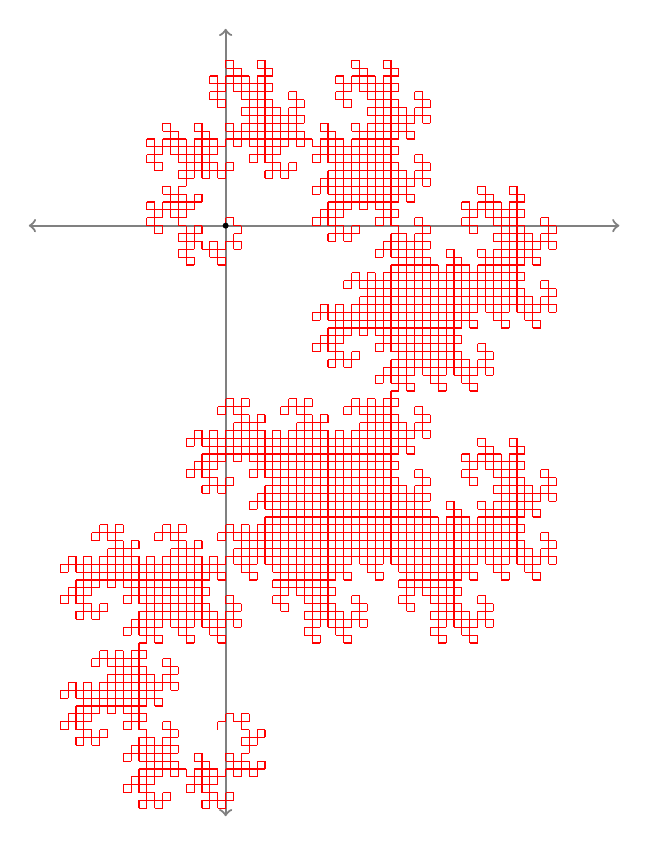
\begin{tikzpicture}[remember picture,scale = 0.1]
\draw[thick, black!50, <->] (-25,0) to (50,0);
\draw[thick, black!50, <->] (0,-75) to (0,25);
\draw[,-,red] (0,0) to (0,1);
\draw[,-,red] (0,1) to (1,1);
\draw[,-,red] (1,1) to (1,0);
\draw[,-,red] (1,0) to (2,0);
\draw[,-,red] (2,0) to (2,-1);
\draw[,-,red] (2,-1) to (1,-1);
\draw[,-,red] (1,-1) to (1,-2);
\draw[,-,red] (1,-2) to (2,-2);
\draw[,-,red] (2,-2) to (2,-3);
\draw[,-,red] (2,-3) to (1,-3);
\draw[,-,red] (1,-3) to (1,-2);
\draw[,-,red] (1,-2) to (0,-2);
\draw[,-,red] (0,-2) to (0,-3);
\draw[,-,red] (0,-3) to (-1,-3);
\draw[,-,red] (-1,-3) to (-1,-4);
\draw[,-,red] (-1,-4) to (0,-4);
\draw[,-,red] (0,-4) to (0,-5);
\draw[,-,red] (0,-5) to (-1,-5);
\draw[,-,red] (-1,-5) to (-1,-4);
\draw[,-,red] (-1,-4) to (-2,-4);
\draw[,-,red] (-2,-4) to (-2,-3);
\draw[,-,red] (-2,-3) to (-1,-3);
\draw[,-,red] (-1,-3) to (-1,-2);
\draw[,-,red] (-1,-2) to (-2,-2);
\draw[,-,red] (-2,-2) to (-2,-3);
\draw[,-,red] (-2,-3) to (-3,-3);
\draw[,-,red] (-3,-3) to (-3,-2);
\draw[,-,red] (-3,-2) to (-4,-2);
\draw[,-,red] (-4,-2) to (-4,-3);
\draw[,-,red] (-4,-3) to (-5,-3);
\draw[,-,red] (-5,-3) to (-5,-4);
\draw[,-,red] (-5,-4) to (-4,-4);
\draw[,-,red] (-4,-4) to (-4,-5);
\draw[,-,red] (-4,-5) to (-5,-5);
\draw[,-,red] (-5,-5) to (-5,-4);
\draw[,-,red] (-5,-4) to (-6,-4);
\draw[,-,red] (-6,-4) to (-6,-3);
\draw[,-,red] (-6,-3) to (-5,-3);
\draw[,-,red] (-5,-3) to (-5,-2);
\draw[,-,red] (-5,-2) to (-6,-2);
\draw[,-,red] (-6,-2) to (-6,-1);
\draw[,-,red] (-6,-1) to (-5,-1);
\draw[,-,red] (-5,-1) to (-5,-2);
\draw[,-,red] (-5,-2) to (-4,-2);
\draw[,-,red] (-4,-2) to (-4,-1);
\draw[,-,red] (-4,-1) to (-3,-1);
\draw[,-,red] (-3,-1) to (-3,0);
\draw[,-,red] (-3,0) to (-4,0);
\draw[,-,red] (-4,0) to (-4,-1);
\draw[,-,red] (-4,-1) to (-5,-1);
\draw[,-,red] (-5,-1) to (-5,0);
\draw[,-,red] (-5,0) to (-6,0);
\draw[,-,red] (-6,0) to (-6,1);
\draw[,-,red] (-6,1) to (-5,1);
\draw[,-,red] (-5,1) to (-5,2);
\draw[,-,red] (-5,2) to (-6,2);
\draw[,-,red] (-6,2) to (-6,1);
\draw[,-,red] (-6,1) to (-7,1);
\draw[,-,red] (-7,1) to (-7,2);
\draw[,-,red] (-7,2) to (-8,2);
\draw[,-,red] (-8,2) to (-8,1);
\draw[,-,red] (-8,1) to (-9,1);
\draw[,-,red] (-9,1) to (-9,0);
\draw[,-,red] (-9,0) to (-8,0);
\draw[,-,red] (-8,0) to (-8,-1);
\draw[,-,red] (-8,-1) to (-9,-1);
\draw[,-,red] (-9,-1) to (-9,0);
\draw[,-,red] (-9,0) to (-10,0);
\draw[,-,red] (-10,0) to (-10,1);
\draw[,-,red] (-10,1) to (-9,1);
\draw[,-,red] (-9,1) to (-9,2);
\draw[,-,red] (-9,2) to (-10,2);
\draw[,-,red] (-10,2) to (-10,3);
\draw[,-,red] (-10,3) to (-9,3);
\draw[,-,red] (-9,3) to (-9,2);
\draw[,-,red] (-9,2) to (-8,2);
\draw[,-,red] (-8,2) to (-8,3);
\draw[,-,red] (-8,3) to (-7,3);
\draw[,-,red] (-7,3) to (-7,4);
\draw[,-,red] (-7,4) to (-8,4);
\draw[,-,red] (-8,4) to (-8,5);
\draw[,-,red] (-8,5) to (-7,5);
\draw[,-,red] (-7,5) to (-7,4);
\draw[,-,red] (-7,4) to (-6,4);
\draw[,-,red] (-6,4) to (-6,3);
\draw[,-,red] (-6,3) to (-7,3);
\draw[,-,red] (-7,3) to (-7,2);
\draw[,-,red] (-7,2) to (-6,2);
\draw[,-,red] (-6,2) to (-6,3);
\draw[,-,red] (-6,3) to (-5,3);
\draw[,-,red] (-5,3) to (-5,2);
\draw[,-,red] (-5,2) to (-4,2);
\draw[,-,red] (-4,2) to (-4,3);
\draw[,-,red] (-4,3) to (-3,3);
\draw[,-,red] (-3,3) to (-3,4);
\draw[,-,red] (-3,4) to (-4,4);
\draw[,-,red] (-4,4) to (-4,3);
\draw[,-,red] (-4,3) to (-5,3);
\draw[,-,red] (-5,3) to (-5,4);
\draw[,-,red] (-5,4) to (-6,4);
\draw[,-,red] (-6,4) to (-6,5);
\draw[,-,red] (-6,5) to (-5,5);
\draw[,-,red] (-5,5) to (-5,6);
\draw[,-,red] (-5,6) to (-6,6);
\draw[,-,red] (-6,6) to (-6,7);
\draw[,-,red] (-6,7) to (-5,7);
\draw[,-,red] (-5,7) to (-5,6);
\draw[,-,red] (-5,6) to (-4,6);
\draw[,-,red] (-4,6) to (-4,7);
\draw[,-,red] (-4,7) to (-3,7);
\draw[,-,red] (-3,7) to (-3,8);
\draw[,-,red] (-3,8) to (-4,8);
\draw[,-,red] (-4,8) to (-4,7);
\draw[,-,red] (-4,7) to (-5,7);
\draw[,-,red] (-5,7) to (-5,8);
\draw[,-,red] (-5,8) to (-6,8);
\draw[,-,red] (-6,8) to (-6,9);
\draw[,-,red] (-6,9) to (-5,9);
\draw[,-,red] (-5,9) to (-5,10);
\draw[,-,red] (-5,10) to (-6,10);
\draw[,-,red] (-6,10) to (-6,9);
\draw[,-,red] (-6,9) to (-7,9);
\draw[,-,red] (-7,9) to (-7,10);
\draw[,-,red] (-7,10) to (-8,10);
\draw[,-,red] (-8,10) to (-8,9);
\draw[,-,red] (-8,9) to (-9,9);
\draw[,-,red] (-9,9) to (-9,8);
\draw[,-,red] (-9,8) to (-8,8);
\draw[,-,red] (-8,8) to (-8,7);
\draw[,-,red] (-8,7) to (-9,7);
\draw[,-,red] (-9,7) to (-9,8);
\draw[,-,red] (-9,8) to (-10,8);
\draw[,-,red] (-10,8) to (-10,9);
\draw[,-,red] (-10,9) to (-9,9);
\draw[,-,red] (-9,9) to (-9,10);
\draw[,-,red] (-9,10) to (-10,10);
\draw[,-,red] (-10,10) to (-10,11);
\draw[,-,red] (-10,11) to (-9,11);
\draw[,-,red] (-9,11) to (-9,10);
\draw[,-,red] (-9,10) to (-8,10);
\draw[,-,red] (-8,10) to (-8,11);
\draw[,-,red] (-8,11) to (-7,11);
\draw[,-,red] (-7,11) to (-7,12);
\draw[,-,red] (-7,12) to (-8,12);
\draw[,-,red] (-8,12) to (-8,13);
\draw[,-,red] (-8,13) to (-7,13);
\draw[,-,red] (-7,13) to (-7,12);
\draw[,-,red] (-7,12) to (-6,12);
\draw[,-,red] (-6,12) to (-6,11);
\draw[,-,red] (-6,11) to (-7,11);
\draw[,-,red] (-7,11) to (-7,10);
\draw[,-,red] (-7,10) to (-6,10);
\draw[,-,red] (-6,10) to (-6,11);
\draw[,-,red] (-6,11) to (-5,11);
\draw[,-,red] (-5,11) to (-5,10);
\draw[,-,red] (-5,10) to (-4,10);
\draw[,-,red] (-4,10) to (-4,11);
\draw[,-,red] (-4,11) to (-3,11);
\draw[,-,red] (-3,11) to (-3,12);
\draw[,-,red] (-3,12) to (-4,12);
\draw[,-,red] (-4,12) to (-4,13);
\draw[,-,red] (-4,13) to (-3,13);
\draw[,-,red] (-3,13) to (-3,12);
\draw[,-,red] (-3,12) to (-2,12);
\draw[,-,red] (-2,12) to (-2,11);
\draw[,-,red] (-2,11) to (-3,11);
\draw[,-,red] (-3,11) to (-3,10);
\draw[,-,red] (-3,10) to (-2,10);
\draw[,-,red] (-2,10) to (-2,9);
\draw[,-,red] (-2,9) to (-3,9);
\draw[,-,red] (-3,9) to (-3,10);
\draw[,-,red] (-3,10) to (-4,10);
\draw[,-,red] (-4,10) to (-4,9);
\draw[,-,red] (-4,9) to (-5,9);
\draw[,-,red] (-5,9) to (-5,8);
\draw[,-,red] (-5,8) to (-4,8);
\draw[,-,red] (-4,8) to (-4,9);
\draw[,-,red] (-4,9) to (-3,9);
\draw[,-,red] (-3,9) to (-3,8);
\draw[,-,red] (-3,8) to (-2,8);
\draw[,-,red] (-2,8) to (-2,7);
\draw[,-,red] (-2,7) to (-3,7);
\draw[,-,red] (-3,7) to (-3,6);
\draw[,-,red] (-3,6) to (-2,6);
\draw[,-,red] (-2,6) to (-2,7);
\draw[,-,red] (-2,7) to (-1,7);
\draw[,-,red] (-1,7) to (-1,6);
\draw[,-,red] (-1,6) to (0,6);
\draw[,-,red] (0,6) to (0,7);
\draw[,-,red] (0,7) to (1,7);
\draw[,-,red] (1,7) to (1,8);
\draw[,-,red] (1,8) to (0,8);
\draw[,-,red] (0,8) to (0,7);
\draw[,-,red] (0,7) to (-1,7);
\draw[,-,red] (-1,7) to (-1,8);
\draw[,-,red] (-1,8) to (-2,8);
\draw[,-,red] (-2,8) to (-2,9);
\draw[,-,red] (-2,9) to (-1,9);
\draw[,-,red] (-1,9) to (-1,10);
\draw[,-,red] (-1,10) to (-2,10);
\draw[,-,red] (-2,10) to (-2,11);
\draw[,-,red] (-2,11) to (-1,11);
\draw[,-,red] (-1,11) to (-1,10);
\draw[,-,red] (-1,10) to (0,10);
\draw[,-,red] (0,10) to (0,11);
\draw[,-,red] (0,11) to (1,11);
\draw[,-,red] (1,11) to (1,12);
\draw[,-,red] (1,12) to (0,12);
\draw[,-,red] (0,12) to (0,13);
\draw[,-,red] (0,13) to (1,13);
\draw[,-,red] (1,13) to (1,12);
\draw[,-,red] (1,12) to (2,12);
\draw[,-,red] (2,12) to (2,11);
\draw[,-,red] (2,11) to (1,11);
\draw[,-,red] (1,11) to (1,10);
\draw[,-,red] (1,10) to (2,10);
\draw[,-,red] (2,10) to (2,11);
\draw[,-,red] (2,11) to (3,11);
\draw[,-,red] (3,11) to (3,10);
\draw[,-,red] (3,10) to (4,10);
\draw[,-,red] (4,10) to (4,11);
\draw[,-,red] (4,11) to (5,11);
\draw[,-,red] (5,11) to (5,12);
\draw[,-,red] (5,12) to (4,12);
\draw[,-,red] (4,12) to (4,11);
\draw[,-,red] (4,11) to (3,11);
\draw[,-,red] (3,11) to (3,12);
\draw[,-,red] (3,12) to (2,12);
\draw[,-,red] (2,12) to (2,13);
\draw[,-,red] (2,13) to (3,13);
\draw[,-,red] (3,13) to (3,14);
\draw[,-,red] (3,14) to (2,14);
\draw[,-,red] (2,14) to (2,15);
\draw[,-,red] (2,15) to (3,15);
\draw[,-,red] (3,15) to (3,14);
\draw[,-,red] (3,14) to (4,14);
\draw[,-,red] (4,14) to (4,15);
\draw[,-,red] (4,15) to (5,15);
\draw[,-,red] (5,15) to (5,16);
\draw[,-,red] (5,16) to (4,16);
\draw[,-,red] (4,16) to (4,15);
\draw[,-,red] (4,15) to (3,15);
\draw[,-,red] (3,15) to (3,16);
\draw[,-,red] (3,16) to (2,16);
\draw[,-,red] (2,16) to (2,17);
\draw[,-,red] (2,17) to (3,17);
\draw[,-,red] (3,17) to (3,18);
\draw[,-,red] (3,18) to (2,18);
\draw[,-,red] (2,18) to (2,17);
\draw[,-,red] (2,17) to (1,17);
\draw[,-,red] (1,17) to (1,18);
\draw[,-,red] (1,18) to (0,18);
\draw[,-,red] (0,18) to (0,17);
\draw[,-,red] (0,17) to (-1,17);
\draw[,-,red] (-1,17) to (-1,16);
\draw[,-,red] (-1,16) to (0,16);
\draw[,-,red] (0,16) to (0,15);
\draw[,-,red] (0,15) to (-1,15);
\draw[,-,red] (-1,15) to (-1,16);
\draw[,-,red] (-1,16) to (-2,16);
\draw[,-,red] (-2,16) to (-2,17);
\draw[,-,red] (-2,17) to (-1,17);
\draw[,-,red] (-1,17) to (-1,18);
\draw[,-,red] (-1,18) to (-2,18);
\draw[,-,red] (-2,18) to (-2,19);
\draw[,-,red] (-2,19) to (-1,19);
\draw[,-,red] (-1,19) to (-1,18);
\draw[,-,red] (-1,18) to (0,18);
\draw[,-,red] (0,18) to (0,19);
\draw[,-,red] (0,19) to (1,19);
\draw[,-,red] (1,19) to (1,20);
\draw[,-,red] (1,20) to (0,20);
\draw[,-,red] (0,20) to (0,21);
\draw[,-,red] (0,21) to (1,21);
\draw[,-,red] (1,21) to (1,20);
\draw[,-,red] (1,20) to (2,20);
\draw[,-,red] (2,20) to (2,19);
\draw[,-,red] (2,19) to (1,19);
\draw[,-,red] (1,19) to (1,18);
\draw[,-,red] (1,18) to (2,18);
\draw[,-,red] (2,18) to (2,19);
\draw[,-,red] (2,19) to (3,19);
\draw[,-,red] (3,19) to (3,18);
\draw[,-,red] (3,18) to (4,18);
\draw[,-,red] (4,18) to (4,19);
\draw[,-,red] (4,19) to (5,19);
\draw[,-,red] (5,19) to (5,20);
\draw[,-,red] (5,20) to (4,20);
\draw[,-,red] (4,20) to (4,21);
\draw[,-,red] (4,21) to (5,21);
\draw[,-,red] (5,21) to (5,20);
\draw[,-,red] (5,20) to (6,20);
\draw[,-,red] (6,20) to (6,19);
\draw[,-,red] (6,19) to (5,19);
\draw[,-,red] (5,19) to (5,18);
\draw[,-,red] (5,18) to (6,18);
\draw[,-,red] (6,18) to (6,17);
\draw[,-,red] (6,17) to (5,17);
\draw[,-,red] (5,17) to (5,18);
\draw[,-,red] (5,18) to (4,18);
\draw[,-,red] (4,18) to (4,17);
\draw[,-,red] (4,17) to (3,17);
\draw[,-,red] (3,17) to (3,16);
\draw[,-,red] (3,16) to (4,16);
\draw[,-,red] (4,16) to (4,17);
\draw[,-,red] (4,17) to (5,17);
\draw[,-,red] (5,17) to (5,16);
\draw[,-,red] (5,16) to (6,16);
\draw[,-,red] (6,16) to (6,15);
\draw[,-,red] (6,15) to (5,15);
\draw[,-,red] (5,15) to (5,14);
\draw[,-,red] (5,14) to (6,14);
\draw[,-,red] (6,14) to (6,15);
\draw[,-,red] (6,15) to (7,15);
\draw[,-,red] (7,15) to (7,14);
\draw[,-,red] (7,14) to (8,14);
\draw[,-,red] (8,14) to (8,15);
\draw[,-,red] (8,15) to (9,15);
\draw[,-,red] (9,15) to (9,16);
\draw[,-,red] (9,16) to (8,16);
\draw[,-,red] (8,16) to (8,17);
\draw[,-,red] (8,17) to (9,17);
\draw[,-,red] (9,17) to (9,16);
\draw[,-,red] (9,16) to (10,16);
\draw[,-,red] (10,16) to (10,15);
\draw[,-,red] (10,15) to (9,15);
\draw[,-,red] (9,15) to (9,14);
\draw[,-,red] (9,14) to (10,14);
\draw[,-,red] (10,14) to (10,13);
\draw[,-,red] (10,13) to (9,13);
\draw[,-,red] (9,13) to (9,14);
\draw[,-,red] (9,14) to (8,14);
\draw[,-,red] (8,14) to (8,13);
\draw[,-,red] (8,13) to (7,13);
\draw[,-,red] (7,13) to (7,12);
\draw[,-,red] (7,12) to (8,12);
\draw[,-,red] (8,12) to (8,11);
\draw[,-,red] (8,11) to (7,11);
\draw[,-,red] (7,11) to (7,12);
\draw[,-,red] (7,12) to (6,12);
\draw[,-,red] (6,12) to (6,13);
\draw[,-,red] (6,13) to (7,13);
\draw[,-,red] (7,13) to (7,14);
\draw[,-,red] (7,14) to (6,14);
\draw[,-,red] (6,14) to (6,13);
\draw[,-,red] (6,13) to (5,13);
\draw[,-,red] (5,13) to (5,14);
\draw[,-,red] (5,14) to (4,14);
\draw[,-,red] (4,14) to (4,13);
\draw[,-,red] (4,13) to (3,13);
\draw[,-,red] (3,13) to (3,12);
\draw[,-,red] (3,12) to (4,12);
\draw[,-,red] (4,12) to (4,13);
\draw[,-,red] (4,13) to (5,13);
\draw[,-,red] (5,13) to (5,12);
\draw[,-,red] (5,12) to (6,12);
\draw[,-,red] (6,12) to (6,11);
\draw[,-,red] (6,11) to (5,11);
\draw[,-,red] (5,11) to (5,10);
\draw[,-,red] (5,10) to (6,10);
\draw[,-,red] (6,10) to (6,9);
\draw[,-,red] (6,9) to (5,9);
\draw[,-,red] (5,9) to (5,10);
\draw[,-,red] (5,10) to (4,10);
\draw[,-,red] (4,10) to (4,9);
\draw[,-,red] (4,9) to (3,9);
\draw[,-,red] (3,9) to (3,8);
\draw[,-,red] (3,8) to (4,8);
\draw[,-,red] (4,8) to (4,9);
\draw[,-,red] (4,9) to (5,9);
\draw[,-,red] (5,9) to (5,8);
\draw[,-,red] (5,8) to (6,8);
\draw[,-,red] (6,8) to (6,7);
\draw[,-,red] (6,7) to (5,7);
\draw[,-,red] (5,7) to (5,6);
\draw[,-,red] (5,6) to (6,6);
\draw[,-,red] (6,6) to (6,7);
\draw[,-,red] (6,7) to (7,7);
\draw[,-,red] (7,7) to (7,6);
\draw[,-,red] (7,6) to (8,6);
\draw[,-,red] (8,6) to (8,7);
\draw[,-,red] (8,7) to (9,7);
\draw[,-,red] (9,7) to (9,8);
\draw[,-,red] (9,8) to (8,8);
\draw[,-,red] (8,8) to (8,7);
\draw[,-,red] (8,7) to (7,7);
\draw[,-,red] (7,7) to (7,8);
\draw[,-,red] (7,8) to (6,8);
\draw[,-,red] (6,8) to (6,9);
\draw[,-,red] (6,9) to (7,9);
\draw[,-,red] (7,9) to (7,10);
\draw[,-,red] (7,10) to (6,10);
\draw[,-,red] (6,10) to (6,11);
\draw[,-,red] (6,11) to (7,11);
\draw[,-,red] (7,11) to (7,10);
\draw[,-,red] (7,10) to (8,10);
\draw[,-,red] (8,10) to (8,11);
\draw[,-,red] (8,11) to (9,11);
\draw[,-,red] (9,11) to (9,12);
\draw[,-,red] (9,12) to (8,12);
\draw[,-,red] (8,12) to (8,13);
\draw[,-,red] (8,13) to (9,13);
\draw[,-,red] (9,13) to (9,12);
\draw[,-,red] (9,12) to (10,12);
\draw[,-,red] (10,12) to (10,11);
\draw[,-,red] (10,11) to (9,11);
\draw[,-,red] (9,11) to (9,10);
\draw[,-,red] (9,10) to (10,10);
\draw[,-,red] (10,10) to (10,11);
\draw[,-,red] (10,11) to (11,11);
\draw[,-,red] (11,11) to (11,10);
\draw[,-,red] (11,10) to (12,10);
\draw[,-,red] (12,10) to (12,11);
\draw[,-,red] (12,11) to (13,11);
\draw[,-,red] (13,11) to (13,12);
\draw[,-,red] (13,12) to (12,12);
\draw[,-,red] (12,12) to (12,13);
\draw[,-,red] (12,13) to (13,13);
\draw[,-,red] (13,13) to (13,12);
\draw[,-,red] (13,12) to (14,12);
\draw[,-,red] (14,12) to (14,11);
\draw[,-,red] (14,11) to (13,11);
\draw[,-,red] (13,11) to (13,10);
\draw[,-,red] (13,10) to (14,10);
\draw[,-,red] (14,10) to (14,9);
\draw[,-,red] (14,9) to (13,9);
\draw[,-,red] (13,9) to (13,10);
\draw[,-,red] (13,10) to (12,10);
\draw[,-,red] (12,10) to (12,9);
\draw[,-,red] (12,9) to (11,9);
\draw[,-,red] (11,9) to (11,8);
\draw[,-,red] (11,8) to (12,8);
\draw[,-,red] (12,8) to (12,9);
\draw[,-,red] (12,9) to (13,9);
\draw[,-,red] (13,9) to (13,8);
\draw[,-,red] (13,8) to (14,8);
\draw[,-,red] (14,8) to (14,7);
\draw[,-,red] (14,7) to (13,7);
\draw[,-,red] (13,7) to (13,6);
\draw[,-,red] (13,6) to (14,6);
\draw[,-,red] (14,6) to (14,7);
\draw[,-,red] (14,7) to (15,7);
\draw[,-,red] (15,7) to (15,6);
\draw[,-,red] (15,6) to (16,6);
\draw[,-,red] (16,6) to (16,7);
\draw[,-,red] (16,7) to (17,7);
\draw[,-,red] (17,7) to (17,8);
\draw[,-,red] (17,8) to (16,8);
\draw[,-,red] (16,8) to (16,7);
\draw[,-,red] (16,7) to (15,7);
\draw[,-,red] (15,7) to (15,8);
\draw[,-,red] (15,8) to (14,8);
\draw[,-,red] (14,8) to (14,9);
\draw[,-,red] (14,9) to (15,9);
\draw[,-,red] (15,9) to (15,10);
\draw[,-,red] (15,10) to (14,10);
\draw[,-,red] (14,10) to (14,11);
\draw[,-,red] (14,11) to (15,11);
\draw[,-,red] (15,11) to (15,10);
\draw[,-,red] (15,10) to (16,10);
\draw[,-,red] (16,10) to (16,11);
\draw[,-,red] (16,11) to (17,11);
\draw[,-,red] (17,11) to (17,12);
\draw[,-,red] (17,12) to (16,12);
\draw[,-,red] (16,12) to (16,13);
\draw[,-,red] (16,13) to (17,13);
\draw[,-,red] (17,13) to (17,12);
\draw[,-,red] (17,12) to (18,12);
\draw[,-,red] (18,12) to (18,11);
\draw[,-,red] (18,11) to (17,11);
\draw[,-,red] (17,11) to (17,10);
\draw[,-,red] (17,10) to (18,10);
\draw[,-,red] (18,10) to (18,11);
\draw[,-,red] (18,11) to (19,11);
\draw[,-,red] (19,11) to (19,10);
\draw[,-,red] (19,10) to (20,10);
\draw[,-,red] (20,10) to (20,11);
\draw[,-,red] (20,11) to (21,11);
\draw[,-,red] (21,11) to (21,12);
\draw[,-,red] (21,12) to (20,12);
\draw[,-,red] (20,12) to (20,11);
\draw[,-,red] (20,11) to (19,11);
\draw[,-,red] (19,11) to (19,12);
\draw[,-,red] (19,12) to (18,12);
\draw[,-,red] (18,12) to (18,13);
\draw[,-,red] (18,13) to (19,13);
\draw[,-,red] (19,13) to (19,14);
\draw[,-,red] (19,14) to (18,14);
\draw[,-,red] (18,14) to (18,15);
\draw[,-,red] (18,15) to (19,15);
\draw[,-,red] (19,15) to (19,14);
\draw[,-,red] (19,14) to (20,14);
\draw[,-,red] (20,14) to (20,15);
\draw[,-,red] (20,15) to (21,15);
\draw[,-,red] (21,15) to (21,16);
\draw[,-,red] (21,16) to (20,16);
\draw[,-,red] (20,16) to (20,15);
\draw[,-,red] (20,15) to (19,15);
\draw[,-,red] (19,15) to (19,16);
\draw[,-,red] (19,16) to (18,16);
\draw[,-,red] (18,16) to (18,17);
\draw[,-,red] (18,17) to (19,17);
\draw[,-,red] (19,17) to (19,18);
\draw[,-,red] (19,18) to (18,18);
\draw[,-,red] (18,18) to (18,17);
\draw[,-,red] (18,17) to (17,17);
\draw[,-,red] (17,17) to (17,18);
\draw[,-,red] (17,18) to (16,18);
\draw[,-,red] (16,18) to (16,17);
\draw[,-,red] (16,17) to (15,17);
\draw[,-,red] (15,17) to (15,16);
\draw[,-,red] (15,16) to (16,16);
\draw[,-,red] (16,16) to (16,15);
\draw[,-,red] (16,15) to (15,15);
\draw[,-,red] (15,15) to (15,16);
\draw[,-,red] (15,16) to (14,16);
\draw[,-,red] (14,16) to (14,17);
\draw[,-,red] (14,17) to (15,17);
\draw[,-,red] (15,17) to (15,18);
\draw[,-,red] (15,18) to (14,18);
\draw[,-,red] (14,18) to (14,19);
\draw[,-,red] (14,19) to (15,19);
\draw[,-,red] (15,19) to (15,18);
\draw[,-,red] (15,18) to (16,18);
\draw[,-,red] (16,18) to (16,19);
\draw[,-,red] (16,19) to (17,19);
\draw[,-,red] (17,19) to (17,20);
\draw[,-,red] (17,20) to (16,20);
\draw[,-,red] (16,20) to (16,21);
\draw[,-,red] (16,21) to (17,21);
\draw[,-,red] (17,21) to (17,20);
\draw[,-,red] (17,20) to (18,20);
\draw[,-,red] (18,20) to (18,19);
\draw[,-,red] (18,19) to (17,19);
\draw[,-,red] (17,19) to (17,18);
\draw[,-,red] (17,18) to (18,18);
\draw[,-,red] (18,18) to (18,19);
\draw[,-,red] (18,19) to (19,19);
\draw[,-,red] (19,19) to (19,18);
\draw[,-,red] (19,18) to (20,18);
\draw[,-,red] (20,18) to (20,19);
\draw[,-,red] (20,19) to (21,19);
\draw[,-,red] (21,19) to (21,20);
\draw[,-,red] (21,20) to (20,20);
\draw[,-,red] (20,20) to (20,21);
\draw[,-,red] (20,21) to (21,21);
\draw[,-,red] (21,21) to (21,20);
\draw[,-,red] (21,20) to (22,20);
\draw[,-,red] (22,20) to (22,19);
\draw[,-,red] (22,19) to (21,19);
\draw[,-,red] (21,19) to (21,18);
\draw[,-,red] (21,18) to (22,18);
\draw[,-,red] (22,18) to (22,17);
\draw[,-,red] (22,17) to (21,17);
\draw[,-,red] (21,17) to (21,18);
\draw[,-,red] (21,18) to (20,18);
\draw[,-,red] (20,18) to (20,17);
\draw[,-,red] (20,17) to (19,17);
\draw[,-,red] (19,17) to (19,16);
\draw[,-,red] (19,16) to (20,16);
\draw[,-,red] (20,16) to (20,17);
\draw[,-,red] (20,17) to (21,17);
\draw[,-,red] (21,17) to (21,16);
\draw[,-,red] (21,16) to (22,16);
\draw[,-,red] (22,16) to (22,15);
\draw[,-,red] (22,15) to (21,15);
\draw[,-,red] (21,15) to (21,14);
\draw[,-,red] (21,14) to (22,14);
\draw[,-,red] (22,14) to (22,15);
\draw[,-,red] (22,15) to (23,15);
\draw[,-,red] (23,15) to (23,14);
\draw[,-,red] (23,14) to (24,14);
\draw[,-,red] (24,14) to (24,15);
\draw[,-,red] (24,15) to (25,15);
\draw[,-,red] (25,15) to (25,16);
\draw[,-,red] (25,16) to (24,16);
\draw[,-,red] (24,16) to (24,17);
\draw[,-,red] (24,17) to (25,17);
\draw[,-,red] (25,17) to (25,16);
\draw[,-,red] (25,16) to (26,16);
\draw[,-,red] (26,16) to (26,15);
\draw[,-,red] (26,15) to (25,15);
\draw[,-,red] (25,15) to (25,14);
\draw[,-,red] (25,14) to (26,14);
\draw[,-,red] (26,14) to (26,13);
\draw[,-,red] (26,13) to (25,13);
\draw[,-,red] (25,13) to (25,14);
\draw[,-,red] (25,14) to (24,14);
\draw[,-,red] (24,14) to (24,13);
\draw[,-,red] (24,13) to (23,13);
\draw[,-,red] (23,13) to (23,12);
\draw[,-,red] (23,12) to (24,12);
\draw[,-,red] (24,12) to (24,11);
\draw[,-,red] (24,11) to (23,11);
\draw[,-,red] (23,11) to (23,12);
\draw[,-,red] (23,12) to (22,12);
\draw[,-,red] (22,12) to (22,13);
\draw[,-,red] (22,13) to (23,13);
\draw[,-,red] (23,13) to (23,14);
\draw[,-,red] (23,14) to (22,14);
\draw[,-,red] (22,14) to (22,13);
\draw[,-,red] (22,13) to (21,13);
\draw[,-,red] (21,13) to (21,14);
\draw[,-,red] (21,14) to (20,14);
\draw[,-,red] (20,14) to (20,13);
\draw[,-,red] (20,13) to (19,13);
\draw[,-,red] (19,13) to (19,12);
\draw[,-,red] (19,12) to (20,12);
\draw[,-,red] (20,12) to (20,13);
\draw[,-,red] (20,13) to (21,13);
\draw[,-,red] (21,13) to (21,12);
\draw[,-,red] (21,12) to (22,12);
\draw[,-,red] (22,12) to (22,11);
\draw[,-,red] (22,11) to (21,11);
\draw[,-,red] (21,11) to (21,10);
\draw[,-,red] (21,10) to (22,10);
\draw[,-,red] (22,10) to (22,9);
\draw[,-,red] (22,9) to (21,9);
\draw[,-,red] (21,9) to (21,10);
\draw[,-,red] (21,10) to (20,10);
\draw[,-,red] (20,10) to (20,9);
\draw[,-,red] (20,9) to (19,9);
\draw[,-,red] (19,9) to (19,8);
\draw[,-,red] (19,8) to (20,8);
\draw[,-,red] (20,8) to (20,9);
\draw[,-,red] (20,9) to (21,9);
\draw[,-,red] (21,9) to (21,8);
\draw[,-,red] (21,8) to (22,8);
\draw[,-,red] (22,8) to (22,7);
\draw[,-,red] (22,7) to (21,7);
\draw[,-,red] (21,7) to (21,6);
\draw[,-,red] (21,6) to (22,6);
\draw[,-,red] (22,6) to (22,7);
\draw[,-,red] (22,7) to (23,7);
\draw[,-,red] (23,7) to (23,6);
\draw[,-,red] (23,6) to (24,6);
\draw[,-,red] (24,6) to (24,7);
\draw[,-,red] (24,7) to (25,7);
\draw[,-,red] (25,7) to (25,8);
\draw[,-,red] (25,8) to (24,8);
\draw[,-,red] (24,8) to (24,9);
\draw[,-,red] (24,9) to (25,9);
\draw[,-,red] (25,9) to (25,8);
\draw[,-,red] (25,8) to (26,8);
\draw[,-,red] (26,8) to (26,7);
\draw[,-,red] (26,7) to (25,7);
\draw[,-,red] (25,7) to (25,6);
\draw[,-,red] (25,6) to (26,6);
\draw[,-,red] (26,6) to (26,5);
\draw[,-,red] (26,5) to (25,5);
\draw[,-,red] (25,5) to (25,6);
\draw[,-,red] (25,6) to (24,6);
\draw[,-,red] (24,6) to (24,5);
\draw[,-,red] (24,5) to (23,5);
\draw[,-,red] (23,5) to (23,4);
\draw[,-,red] (23,4) to (24,4);
\draw[,-,red] (24,4) to (24,3);
\draw[,-,red] (24,3) to (23,3);
\draw[,-,red] (23,3) to (23,4);
\draw[,-,red] (23,4) to (22,4);
\draw[,-,red] (22,4) to (22,5);
\draw[,-,red] (22,5) to (23,5);
\draw[,-,red] (23,5) to (23,6);
\draw[,-,red] (23,6) to (22,6);
\draw[,-,red] (22,6) to (22,5);
\draw[,-,red] (22,5) to (21,5);
\draw[,-,red] (21,5) to (21,6);
\draw[,-,red] (21,6) to (20,6);
\draw[,-,red] (20,6) to (20,5);
\draw[,-,red] (20,5) to (19,5);
\draw[,-,red] (19,5) to (19,4);
\draw[,-,red] (19,4) to (20,4);
\draw[,-,red] (20,4) to (20,3);
\draw[,-,red] (20,3) to (19,3);
\draw[,-,red] (19,3) to (19,4);
\draw[,-,red] (19,4) to (18,4);
\draw[,-,red] (18,4) to (18,5);
\draw[,-,red] (18,5) to (19,5);
\draw[,-,red] (19,5) to (19,6);
\draw[,-,red] (19,6) to (18,6);
\draw[,-,red] (18,6) to (18,7);
\draw[,-,red] (18,7) to (19,7);
\draw[,-,red] (19,7) to (19,6);
\draw[,-,red] (19,6) to (20,6);
\draw[,-,red] (20,6) to (20,7);
\draw[,-,red] (20,7) to (21,7);
\draw[,-,red] (21,7) to (21,8);
\draw[,-,red] (21,8) to (20,8);
\draw[,-,red] (20,8) to (20,7);
\draw[,-,red] (20,7) to (19,7);
\draw[,-,red] (19,7) to (19,8);
\draw[,-,red] (19,8) to (18,8);
\draw[,-,red] (18,8) to (18,9);
\draw[,-,red] (18,9) to (19,9);
\draw[,-,red] (19,9) to (19,10);
\draw[,-,red] (19,10) to (18,10);
\draw[,-,red] (18,10) to (18,9);
\draw[,-,red] (18,9) to (17,9);
\draw[,-,red] (17,9) to (17,10);
\draw[,-,red] (17,10) to (16,10);
\draw[,-,red] (16,10) to (16,9);
\draw[,-,red] (16,9) to (15,9);
\draw[,-,red] (15,9) to (15,8);
\draw[,-,red] (15,8) to (16,8);
\draw[,-,red] (16,8) to (16,9);
\draw[,-,red] (16,9) to (17,9);
\draw[,-,red] (17,9) to (17,8);
\draw[,-,red] (17,8) to (18,8);
\draw[,-,red] (18,8) to (18,7);
\draw[,-,red] (18,7) to (17,7);
\draw[,-,red] (17,7) to (17,6);
\draw[,-,red] (17,6) to (18,6);
\draw[,-,red] (18,6) to (18,5);
\draw[,-,red] (18,5) to (17,5);
\draw[,-,red] (17,5) to (17,6);
\draw[,-,red] (17,6) to (16,6);
\draw[,-,red] (16,6) to (16,5);
\draw[,-,red] (16,5) to (15,5);
\draw[,-,red] (15,5) to (15,4);
\draw[,-,red] (15,4) to (16,4);
\draw[,-,red] (16,4) to (16,3);
\draw[,-,red] (16,3) to (15,3);
\draw[,-,red] (15,3) to (15,4);
\draw[,-,red] (15,4) to (14,4);
\draw[,-,red] (14,4) to (14,5);
\draw[,-,red] (14,5) to (15,5);
\draw[,-,red] (15,5) to (15,6);
\draw[,-,red] (15,6) to (14,6);
\draw[,-,red] (14,6) to (14,5);
\draw[,-,red] (14,5) to (13,5);
\draw[,-,red] (13,5) to (13,6);
\draw[,-,red] (13,6) to (12,6);
\draw[,-,red] (12,6) to (12,5);
\draw[,-,red] (12,5) to (11,5);
\draw[,-,red] (11,5) to (11,4);
\draw[,-,red] (11,4) to (12,4);
\draw[,-,red] (12,4) to (12,5);
\draw[,-,red] (12,5) to (13,5);
\draw[,-,red] (13,5) to (13,4);
\draw[,-,red] (13,4) to (14,4);
\draw[,-,red] (14,4) to (14,3);
\draw[,-,red] (14,3) to (13,3);
\draw[,-,red] (13,3) to (13,2);
\draw[,-,red] (13,2) to (14,2);
\draw[,-,red] (14,2) to (14,1);
\draw[,-,red] (14,1) to (13,1);
\draw[,-,red] (13,1) to (13,2);
\draw[,-,red] (13,2) to (12,2);
\draw[,-,red] (12,2) to (12,1);
\draw[,-,red] (12,1) to (11,1);
\draw[,-,red] (11,1) to (11,0);
\draw[,-,red] (11,0) to (12,0);
\draw[,-,red] (12,0) to (12,1);
\draw[,-,red] (12,1) to (13,1);
\draw[,-,red] (13,1) to (13,0);
\draw[,-,red] (13,0) to (14,0);
\draw[,-,red] (14,0) to (14,-1);
\draw[,-,red] (14,-1) to (13,-1);
\draw[,-,red] (13,-1) to (13,-2);
\draw[,-,red] (13,-2) to (14,-2);
\draw[,-,red] (14,-2) to (14,-1);
\draw[,-,red] (14,-1) to (15,-1);
\draw[,-,red] (15,-1) to (15,-2);
\draw[,-,red] (15,-2) to (16,-2);
\draw[,-,red] (16,-2) to (16,-1);
\draw[,-,red] (16,-1) to (17,-1);
\draw[,-,red] (17,-1) to (17,0);
\draw[,-,red] (17,0) to (16,0);
\draw[,-,red] (16,0) to (16,-1);
\draw[,-,red] (16,-1) to (15,-1);
\draw[,-,red] (15,-1) to (15,0);
\draw[,-,red] (15,0) to (14,0);
\draw[,-,red] (14,0) to (14,1);
\draw[,-,red] (14,1) to (15,1);
\draw[,-,red] (15,1) to (15,2);
\draw[,-,red] (15,2) to (14,2);
\draw[,-,red] (14,2) to (14,3);
\draw[,-,red] (14,3) to (15,3);
\draw[,-,red] (15,3) to (15,2);
\draw[,-,red] (15,2) to (16,2);
\draw[,-,red] (16,2) to (16,3);
\draw[,-,red] (16,3) to (17,3);
\draw[,-,red] (17,3) to (17,4);
\draw[,-,red] (17,4) to (16,4);
\draw[,-,red] (16,4) to (16,5);
\draw[,-,red] (16,5) to (17,5);
\draw[,-,red] (17,5) to (17,4);
\draw[,-,red] (17,4) to (18,4);
\draw[,-,red] (18,4) to (18,3);
\draw[,-,red] (18,3) to (17,3);
\draw[,-,red] (17,3) to (17,2);
\draw[,-,red] (17,2) to (18,2);
\draw[,-,red] (18,2) to (18,3);
\draw[,-,red] (18,3) to (19,3);
\draw[,-,red] (19,3) to (19,2);
\draw[,-,red] (19,2) to (20,2);
\draw[,-,red] (20,2) to (20,3);
\draw[,-,red] (20,3) to (21,3);
\draw[,-,red] (21,3) to (21,4);
\draw[,-,red] (21,4) to (20,4);
\draw[,-,red] (20,4) to (20,5);
\draw[,-,red] (20,5) to (21,5);
\draw[,-,red] (21,5) to (21,4);
\draw[,-,red] (21,4) to (22,4);
\draw[,-,red] (22,4) to (22,3);
\draw[,-,red] (22,3) to (21,3);
\draw[,-,red] (21,3) to (21,2);
\draw[,-,red] (21,2) to (22,2);
\draw[,-,red] (22,2) to (22,1);
\draw[,-,red] (22,1) to (21,1);
\draw[,-,red] (21,1) to (21,2);
\draw[,-,red] (21,2) to (20,2);
\draw[,-,red] (20,2) to (20,1);
\draw[,-,red] (20,1) to (19,1);
\draw[,-,red] (19,1) to (19,0);
\draw[,-,red] (19,0) to (20,0);
\draw[,-,red] (20,0) to (20,1);
\draw[,-,red] (20,1) to (21,1);
\draw[,-,red] (21,1) to (21,0);
\draw[,-,red] (21,0) to (22,0);
\draw[,-,red] (22,0) to (22,-1);
\draw[,-,red] (22,-1) to (21,-1);
\draw[,-,red] (21,-1) to (21,-2);
\draw[,-,red] (21,-2) to (22,-2);
\draw[,-,red] (22,-2) to (22,-1);
\draw[,-,red] (22,-1) to (23,-1);
\draw[,-,red] (23,-1) to (23,-2);
\draw[,-,red] (23,-2) to (24,-2);
\draw[,-,red] (24,-2) to (24,-1);
\draw[,-,red] (24,-1) to (25,-1);
\draw[,-,red] (25,-1) to (25,0);
\draw[,-,red] (25,0) to (24,0);
\draw[,-,red] (24,0) to (24,1);
\draw[,-,red] (24,1) to (25,1);
\draw[,-,red] (25,1) to (25,0);
\draw[,-,red] (25,0) to (26,0);
\draw[,-,red] (26,0) to (26,-1);
\draw[,-,red] (26,-1) to (25,-1);
\draw[,-,red] (25,-1) to (25,-2);
\draw[,-,red] (25,-2) to (26,-2);
\draw[,-,red] (26,-2) to (26,-3);
\draw[,-,red] (26,-3) to (25,-3);
\draw[,-,red] (25,-3) to (25,-2);
\draw[,-,red] (25,-2) to (24,-2);
\draw[,-,red] (24,-2) to (24,-3);
\draw[,-,red] (24,-3) to (23,-3);
\draw[,-,red] (23,-3) to (23,-4);
\draw[,-,red] (23,-4) to (24,-4);
\draw[,-,red] (24,-4) to (24,-5);
\draw[,-,red] (24,-5) to (23,-5);
\draw[,-,red] (23,-5) to (23,-4);
\draw[,-,red] (23,-4) to (22,-4);
\draw[,-,red] (22,-4) to (22,-3);
\draw[,-,red] (22,-3) to (23,-3);
\draw[,-,red] (23,-3) to (23,-2);
\draw[,-,red] (23,-2) to (22,-2);
\draw[,-,red] (22,-2) to (22,-3);
\draw[,-,red] (22,-3) to (21,-3);
\draw[,-,red] (21,-3) to (21,-2);
\draw[,-,red] (21,-2) to (20,-2);
\draw[,-,red] (20,-2) to (20,-3);
\draw[,-,red] (20,-3) to (19,-3);
\draw[,-,red] (19,-3) to (19,-4);
\draw[,-,red] (19,-4) to (20,-4);
\draw[,-,red] (20,-4) to (20,-3);
\draw[,-,red] (20,-3) to (21,-3);
\draw[,-,red] (21,-3) to (21,-4);
\draw[,-,red] (21,-4) to (22,-4);
\draw[,-,red] (22,-4) to (22,-5);
\draw[,-,red] (22,-5) to (21,-5);
\draw[,-,red] (21,-5) to (21,-6);
\draw[,-,red] (21,-6) to (22,-6);
\draw[,-,red] (22,-6) to (22,-7);
\draw[,-,red] (22,-7) to (21,-7);
\draw[,-,red] (21,-7) to (21,-6);
\draw[,-,red] (21,-6) to (20,-6);
\draw[,-,red] (20,-6) to (20,-7);
\draw[,-,red] (20,-7) to (19,-7);
\draw[,-,red] (19,-7) to (19,-8);
\draw[,-,red] (19,-8) to (20,-8);
\draw[,-,red] (20,-8) to (20,-7);
\draw[,-,red] (20,-7) to (21,-7);
\draw[,-,red] (21,-7) to (21,-8);
\draw[,-,red] (21,-8) to (22,-8);
\draw[,-,red] (22,-8) to (22,-9);
\draw[,-,red] (22,-9) to (21,-9);
\draw[,-,red] (21,-9) to (21,-10);
\draw[,-,red] (21,-10) to (22,-10);
\draw[,-,red] (22,-10) to (22,-9);
\draw[,-,red] (22,-9) to (23,-9);
\draw[,-,red] (23,-9) to (23,-10);
\draw[,-,red] (23,-10) to (24,-10);
\draw[,-,red] (24,-10) to (24,-9);
\draw[,-,red] (24,-9) to (25,-9);
\draw[,-,red] (25,-9) to (25,-8);
\draw[,-,red] (25,-8) to (24,-8);
\draw[,-,red] (24,-8) to (24,-9);
\draw[,-,red] (24,-9) to (23,-9);
\draw[,-,red] (23,-9) to (23,-8);
\draw[,-,red] (23,-8) to (22,-8);
\draw[,-,red] (22,-8) to (22,-7);
\draw[,-,red] (22,-7) to (23,-7);
\draw[,-,red] (23,-7) to (23,-6);
\draw[,-,red] (23,-6) to (22,-6);
\draw[,-,red] (22,-6) to (22,-5);
\draw[,-,red] (22,-5) to (23,-5);
\draw[,-,red] (23,-5) to (23,-6);
\draw[,-,red] (23,-6) to (24,-6);
\draw[,-,red] (24,-6) to (24,-5);
\draw[,-,red] (24,-5) to (25,-5);
\draw[,-,red] (25,-5) to (25,-4);
\draw[,-,red] (25,-4) to (24,-4);
\draw[,-,red] (24,-4) to (24,-3);
\draw[,-,red] (24,-3) to (25,-3);
\draw[,-,red] (25,-3) to (25,-4);
\draw[,-,red] (25,-4) to (26,-4);
\draw[,-,red] (26,-4) to (26,-5);
\draw[,-,red] (26,-5) to (25,-5);
\draw[,-,red] (25,-5) to (25,-6);
\draw[,-,red] (25,-6) to (26,-6);
\draw[,-,red] (26,-6) to (26,-5);
\draw[,-,red] (26,-5) to (27,-5);
\draw[,-,red] (27,-5) to (27,-6);
\draw[,-,red] (27,-6) to (28,-6);
\draw[,-,red] (28,-6) to (28,-5);
\draw[,-,red] (28,-5) to (29,-5);
\draw[,-,red] (29,-5) to (29,-4);
\draw[,-,red] (29,-4) to (28,-4);
\draw[,-,red] (28,-4) to (28,-3);
\draw[,-,red] (28,-3) to (29,-3);
\draw[,-,red] (29,-3) to (29,-4);
\draw[,-,red] (29,-4) to (30,-4);
\draw[,-,red] (30,-4) to (30,-5);
\draw[,-,red] (30,-5) to (29,-5);
\draw[,-,red] (29,-5) to (29,-6);
\draw[,-,red] (29,-6) to (30,-6);
\draw[,-,red] (30,-6) to (30,-7);
\draw[,-,red] (30,-7) to (29,-7);
\draw[,-,red] (29,-7) to (29,-6);
\draw[,-,red] (29,-6) to (28,-6);
\draw[,-,red] (28,-6) to (28,-7);
\draw[,-,red] (28,-7) to (27,-7);
\draw[,-,red] (27,-7) to (27,-8);
\draw[,-,red] (27,-8) to (28,-8);
\draw[,-,red] (28,-8) to (28,-7);
\draw[,-,red] (28,-7) to (29,-7);
\draw[,-,red] (29,-7) to (29,-8);
\draw[,-,red] (29,-8) to (30,-8);
\draw[,-,red] (30,-8) to (30,-9);
\draw[,-,red] (30,-9) to (29,-9);
\draw[,-,red] (29,-9) to (29,-10);
\draw[,-,red] (29,-10) to (30,-10);
\draw[,-,red] (30,-10) to (30,-9);
\draw[,-,red] (30,-9) to (31,-9);
\draw[,-,red] (31,-9) to (31,-10);
\draw[,-,red] (31,-10) to (32,-10);
\draw[,-,red] (32,-10) to (32,-9);
\draw[,-,red] (32,-9) to (33,-9);
\draw[,-,red] (33,-9) to (33,-8);
\draw[,-,red] (33,-8) to (32,-8);
\draw[,-,red] (32,-8) to (32,-9);
\draw[,-,red] (32,-9) to (31,-9);
\draw[,-,red] (31,-9) to (31,-8);
\draw[,-,red] (31,-8) to (30,-8);
\draw[,-,red] (30,-8) to (30,-7);
\draw[,-,red] (30,-7) to (31,-7);
\draw[,-,red] (31,-7) to (31,-6);
\draw[,-,red] (31,-6) to (30,-6);
\draw[,-,red] (30,-6) to (30,-5);
\draw[,-,red] (30,-5) to (31,-5);
\draw[,-,red] (31,-5) to (31,-6);
\draw[,-,red] (31,-6) to (32,-6);
\draw[,-,red] (32,-6) to (32,-5);
\draw[,-,red] (32,-5) to (33,-5);
\draw[,-,red] (33,-5) to (33,-4);
\draw[,-,red] (33,-4) to (32,-4);
\draw[,-,red] (32,-4) to (32,-3);
\draw[,-,red] (32,-3) to (33,-3);
\draw[,-,red] (33,-3) to (33,-4);
\draw[,-,red] (33,-4) to (34,-4);
\draw[,-,red] (34,-4) to (34,-5);
\draw[,-,red] (34,-5) to (33,-5);
\draw[,-,red] (33,-5) to (33,-6);
\draw[,-,red] (33,-6) to (34,-6);
\draw[,-,red] (34,-6) to (34,-5);
\draw[,-,red] (34,-5) to (35,-5);
\draw[,-,red] (35,-5) to (35,-6);
\draw[,-,red] (35,-6) to (36,-6);
\draw[,-,red] (36,-6) to (36,-5);
\draw[,-,red] (36,-5) to (37,-5);
\draw[,-,red] (37,-5) to (37,-4);
\draw[,-,red] (37,-4) to (36,-4);
\draw[,-,red] (36,-4) to (36,-5);
\draw[,-,red] (36,-5) to (35,-5);
\draw[,-,red] (35,-5) to (35,-4);
\draw[,-,red] (35,-4) to (34,-4);
\draw[,-,red] (34,-4) to (34,-3);
\draw[,-,red] (34,-3) to (35,-3);
\draw[,-,red] (35,-3) to (35,-2);
\draw[,-,red] (35,-2) to (34,-2);
\draw[,-,red] (34,-2) to (34,-1);
\draw[,-,red] (34,-1) to (35,-1);
\draw[,-,red] (35,-1) to (35,-2);
\draw[,-,red] (35,-2) to (36,-2);
\draw[,-,red] (36,-2) to (36,-1);
\draw[,-,red] (36,-1) to (37,-1);
\draw[,-,red] (37,-1) to (37,0);
\draw[,-,red] (37,0) to (36,0);
\draw[,-,red] (36,0) to (36,-1);
\draw[,-,red] (36,-1) to (35,-1);
\draw[,-,red] (35,-1) to (35,0);
\draw[,-,red] (35,0) to (34,0);
\draw[,-,red] (34,0) to (34,1);
\draw[,-,red] (34,1) to (35,1);
\draw[,-,red] (35,1) to (35,2);
\draw[,-,red] (35,2) to (34,2);
\draw[,-,red] (34,2) to (34,1);
\draw[,-,red] (34,1) to (33,1);
\draw[,-,red] (33,1) to (33,2);
\draw[,-,red] (33,2) to (32,2);
\draw[,-,red] (32,2) to (32,1);
\draw[,-,red] (32,1) to (31,1);
\draw[,-,red] (31,1) to (31,0);
\draw[,-,red] (31,0) to (32,0);
\draw[,-,red] (32,0) to (32,-1);
\draw[,-,red] (32,-1) to (31,-1);
\draw[,-,red] (31,-1) to (31,0);
\draw[,-,red] (31,0) to (30,0);
\draw[,-,red] (30,0) to (30,1);
\draw[,-,red] (30,1) to (31,1);
\draw[,-,red] (31,1) to (31,2);
\draw[,-,red] (31,2) to (30,2);
\draw[,-,red] (30,2) to (30,3);
\draw[,-,red] (30,3) to (31,3);
\draw[,-,red] (31,3) to (31,2);
\draw[,-,red] (31,2) to (32,2);
\draw[,-,red] (32,2) to (32,3);
\draw[,-,red] (32,3) to (33,3);
\draw[,-,red] (33,3) to (33,4);
\draw[,-,red] (33,4) to (32,4);
\draw[,-,red] (32,4) to (32,5);
\draw[,-,red] (32,5) to (33,5);
\draw[,-,red] (33,5) to (33,4);
\draw[,-,red] (33,4) to (34,4);
\draw[,-,red] (34,4) to (34,3);
\draw[,-,red] (34,3) to (33,3);
\draw[,-,red] (33,3) to (33,2);
\draw[,-,red] (33,2) to (34,2);
\draw[,-,red] (34,2) to (34,3);
\draw[,-,red] (34,3) to (35,3);
\draw[,-,red] (35,3) to (35,2);
\draw[,-,red] (35,2) to (36,2);
\draw[,-,red] (36,2) to (36,3);
\draw[,-,red] (36,3) to (37,3);
\draw[,-,red] (37,3) to (37,4);
\draw[,-,red] (37,4) to (36,4);
\draw[,-,red] (36,4) to (36,5);
\draw[,-,red] (36,5) to (37,5);
\draw[,-,red] (37,5) to (37,4);
\draw[,-,red] (37,4) to (38,4);
\draw[,-,red] (38,4) to (38,3);
\draw[,-,red] (38,3) to (37,3);
\draw[,-,red] (37,3) to (37,2);
\draw[,-,red] (37,2) to (38,2);
\draw[,-,red] (38,2) to (38,1);
\draw[,-,red] (38,1) to (37,1);
\draw[,-,red] (37,1) to (37,2);
\draw[,-,red] (37,2) to (36,2);
\draw[,-,red] (36,2) to (36,1);
\draw[,-,red] (36,1) to (35,1);
\draw[,-,red] (35,1) to (35,0);
\draw[,-,red] (35,0) to (36,0);
\draw[,-,red] (36,0) to (36,1);
\draw[,-,red] (36,1) to (37,1);
\draw[,-,red] (37,1) to (37,0);
\draw[,-,red] (37,0) to (38,0);
\draw[,-,red] (38,0) to (38,-1);
\draw[,-,red] (38,-1) to (37,-1);
\draw[,-,red] (37,-1) to (37,-2);
\draw[,-,red] (37,-2) to (38,-2);
\draw[,-,red] (38,-2) to (38,-1);
\draw[,-,red] (38,-1) to (39,-1);
\draw[,-,red] (39,-1) to (39,-2);
\draw[,-,red] (39,-2) to (40,-2);
\draw[,-,red] (40,-2) to (40,-1);
\draw[,-,red] (40,-1) to (41,-1);
\draw[,-,red] (41,-1) to (41,0);
\draw[,-,red] (41,0) to (40,0);
\draw[,-,red] (40,0) to (40,1);
\draw[,-,red] (40,1) to (41,1);
\draw[,-,red] (41,1) to (41,0);
\draw[,-,red] (41,0) to (42,0);
\draw[,-,red] (42,0) to (42,-1);
\draw[,-,red] (42,-1) to (41,-1);
\draw[,-,red] (41,-1) to (41,-2);
\draw[,-,red] (41,-2) to (42,-2);
\draw[,-,red] (42,-2) to (42,-3);
\draw[,-,red] (42,-3) to (41,-3);
\draw[,-,red] (41,-3) to (41,-2);
\draw[,-,red] (41,-2) to (40,-2);
\draw[,-,red] (40,-2) to (40,-3);
\draw[,-,red] (40,-3) to (39,-3);
\draw[,-,red] (39,-3) to (39,-4);
\draw[,-,red] (39,-4) to (40,-4);
\draw[,-,red] (40,-4) to (40,-5);
\draw[,-,red] (40,-5) to (39,-5);
\draw[,-,red] (39,-5) to (39,-4);
\draw[,-,red] (39,-4) to (38,-4);
\draw[,-,red] (38,-4) to (38,-3);
\draw[,-,red] (38,-3) to (39,-3);
\draw[,-,red] (39,-3) to (39,-2);
\draw[,-,red] (39,-2) to (38,-2);
\draw[,-,red] (38,-2) to (38,-3);
\draw[,-,red] (38,-3) to (37,-3);
\draw[,-,red] (37,-3) to (37,-2);
\draw[,-,red] (37,-2) to (36,-2);
\draw[,-,red] (36,-2) to (36,-3);
\draw[,-,red] (36,-3) to (35,-3);
\draw[,-,red] (35,-3) to (35,-4);
\draw[,-,red] (35,-4) to (36,-4);
\draw[,-,red] (36,-4) to (36,-3);
\draw[,-,red] (36,-3) to (37,-3);
\draw[,-,red] (37,-3) to (37,-4);
\draw[,-,red] (37,-4) to (38,-4);
\draw[,-,red] (38,-4) to (38,-5);
\draw[,-,red] (38,-5) to (37,-5);
\draw[,-,red] (37,-5) to (37,-6);
\draw[,-,red] (37,-6) to (38,-6);
\draw[,-,red] (38,-6) to (38,-7);
\draw[,-,red] (38,-7) to (37,-7);
\draw[,-,red] (37,-7) to (37,-6);
\draw[,-,red] (37,-6) to (36,-6);
\draw[,-,red] (36,-6) to (36,-7);
\draw[,-,red] (36,-7) to (35,-7);
\draw[,-,red] (35,-7) to (35,-8);
\draw[,-,red] (35,-8) to (36,-8);
\draw[,-,red] (36,-8) to (36,-7);
\draw[,-,red] (36,-7) to (37,-7);
\draw[,-,red] (37,-7) to (37,-8);
\draw[,-,red] (37,-8) to (38,-8);
\draw[,-,red] (38,-8) to (38,-9);
\draw[,-,red] (38,-9) to (37,-9);
\draw[,-,red] (37,-9) to (37,-10);
\draw[,-,red] (37,-10) to (38,-10);
\draw[,-,red] (38,-10) to (38,-9);
\draw[,-,red] (38,-9) to (39,-9);
\draw[,-,red] (39,-9) to (39,-10);
\draw[,-,red] (39,-10) to (40,-10);
\draw[,-,red] (40,-10) to (40,-9);
\draw[,-,red] (40,-9) to (41,-9);
\draw[,-,red] (41,-9) to (41,-8);
\draw[,-,red] (41,-8) to (40,-8);
\draw[,-,red] (40,-8) to (40,-7);
\draw[,-,red] (40,-7) to (41,-7);
\draw[,-,red] (41,-7) to (41,-8);
\draw[,-,red] (41,-8) to (42,-8);
\draw[,-,red] (42,-8) to (42,-9);
\draw[,-,red] (42,-9) to (41,-9);
\draw[,-,red] (41,-9) to (41,-10);
\draw[,-,red] (41,-10) to (42,-10);
\draw[,-,red] (42,-10) to (42,-11);
\draw[,-,red] (42,-11) to (41,-11);
\draw[,-,red] (41,-11) to (41,-10);
\draw[,-,red] (41,-10) to (40,-10);
\draw[,-,red] (40,-10) to (40,-11);
\draw[,-,red] (40,-11) to (39,-11);
\draw[,-,red] (39,-11) to (39,-12);
\draw[,-,red] (39,-12) to (40,-12);
\draw[,-,red] (40,-12) to (40,-13);
\draw[,-,red] (40,-13) to (39,-13);
\draw[,-,red] (39,-13) to (39,-12);
\draw[,-,red] (39,-12) to (38,-12);
\draw[,-,red] (38,-12) to (38,-11);
\draw[,-,red] (38,-11) to (39,-11);
\draw[,-,red] (39,-11) to (39,-10);
\draw[,-,red] (39,-10) to (38,-10);
\draw[,-,red] (38,-10) to (38,-11);
\draw[,-,red] (38,-11) to (37,-11);
\draw[,-,red] (37,-11) to (37,-10);
\draw[,-,red] (37,-10) to (36,-10);
\draw[,-,red] (36,-10) to (36,-11);
\draw[,-,red] (36,-11) to (35,-11);
\draw[,-,red] (35,-11) to (35,-12);
\draw[,-,red] (35,-12) to (36,-12);
\draw[,-,red] (36,-12) to (36,-13);
\draw[,-,red] (36,-13) to (35,-13);
\draw[,-,red] (35,-13) to (35,-12);
\draw[,-,red] (35,-12) to (34,-12);
\draw[,-,red] (34,-12) to (34,-11);
\draw[,-,red] (34,-11) to (35,-11);
\draw[,-,red] (35,-11) to (35,-10);
\draw[,-,red] (35,-10) to (34,-10);
\draw[,-,red] (34,-10) to (34,-9);
\draw[,-,red] (34,-9) to (35,-9);
\draw[,-,red] (35,-9) to (35,-10);
\draw[,-,red] (35,-10) to (36,-10);
\draw[,-,red] (36,-10) to (36,-9);
\draw[,-,red] (36,-9) to (37,-9);
\draw[,-,red] (37,-9) to (37,-8);
\draw[,-,red] (37,-8) to (36,-8);
\draw[,-,red] (36,-8) to (36,-9);
\draw[,-,red] (36,-9) to (35,-9);
\draw[,-,red] (35,-9) to (35,-8);
\draw[,-,red] (35,-8) to (34,-8);
\draw[,-,red] (34,-8) to (34,-7);
\draw[,-,red] (34,-7) to (35,-7);
\draw[,-,red] (35,-7) to (35,-6);
\draw[,-,red] (35,-6) to (34,-6);
\draw[,-,red] (34,-6) to (34,-7);
\draw[,-,red] (34,-7) to (33,-7);
\draw[,-,red] (33,-7) to (33,-6);
\draw[,-,red] (33,-6) to (32,-6);
\draw[,-,red] (32,-6) to (32,-7);
\draw[,-,red] (32,-7) to (31,-7);
\draw[,-,red] (31,-7) to (31,-8);
\draw[,-,red] (31,-8) to (32,-8);
\draw[,-,red] (32,-8) to (32,-7);
\draw[,-,red] (32,-7) to (33,-7);
\draw[,-,red] (33,-7) to (33,-8);
\draw[,-,red] (33,-8) to (34,-8);
\draw[,-,red] (34,-8) to (34,-9);
\draw[,-,red] (34,-9) to (33,-9);
\draw[,-,red] (33,-9) to (33,-10);
\draw[,-,red] (33,-10) to (34,-10);
\draw[,-,red] (34,-10) to (34,-11);
\draw[,-,red] (34,-11) to (33,-11);
\draw[,-,red] (33,-11) to (33,-10);
\draw[,-,red] (33,-10) to (32,-10);
\draw[,-,red] (32,-10) to (32,-11);
\draw[,-,red] (32,-11) to (31,-11);
\draw[,-,red] (31,-11) to (31,-12);
\draw[,-,red] (31,-12) to (32,-12);
\draw[,-,red] (32,-12) to (32,-13);
\draw[,-,red] (32,-13) to (31,-13);
\draw[,-,red] (31,-13) to (31,-12);
\draw[,-,red] (31,-12) to (30,-12);
\draw[,-,red] (30,-12) to (30,-11);
\draw[,-,red] (30,-11) to (31,-11);
\draw[,-,red] (31,-11) to (31,-10);
\draw[,-,red] (31,-10) to (30,-10);
\draw[,-,red] (30,-10) to (30,-11);
\draw[,-,red] (30,-11) to (29,-11);
\draw[,-,red] (29,-11) to (29,-10);
\draw[,-,red] (29,-10) to (28,-10);
\draw[,-,red] (28,-10) to (28,-11);
\draw[,-,red] (28,-11) to (27,-11);
\draw[,-,red] (27,-11) to (27,-12);
\draw[,-,red] (27,-12) to (28,-12);
\draw[,-,red] (28,-12) to (28,-11);
\draw[,-,red] (28,-11) to (29,-11);
\draw[,-,red] (29,-11) to (29,-12);
\draw[,-,red] (29,-12) to (30,-12);
\draw[,-,red] (30,-12) to (30,-13);
\draw[,-,red] (30,-13) to (29,-13);
\draw[,-,red] (29,-13) to (29,-14);
\draw[,-,red] (29,-14) to (30,-14);
\draw[,-,red] (30,-14) to (30,-15);
\draw[,-,red] (30,-15) to (29,-15);
\draw[,-,red] (29,-15) to (29,-14);
\draw[,-,red] (29,-14) to (28,-14);
\draw[,-,red] (28,-14) to (28,-15);
\draw[,-,red] (28,-15) to (27,-15);
\draw[,-,red] (27,-15) to (27,-16);
\draw[,-,red] (27,-16) to (28,-16);
\draw[,-,red] (28,-16) to (28,-15);
\draw[,-,red] (28,-15) to (29,-15);
\draw[,-,red] (29,-15) to (29,-16);
\draw[,-,red] (29,-16) to (30,-16);
\draw[,-,red] (30,-16) to (30,-17);
\draw[,-,red] (30,-17) to (29,-17);
\draw[,-,red] (29,-17) to (29,-18);
\draw[,-,red] (29,-18) to (30,-18);
\draw[,-,red] (30,-18) to (30,-17);
\draw[,-,red] (30,-17) to (31,-17);
\draw[,-,red] (31,-17) to (31,-18);
\draw[,-,red] (31,-18) to (32,-18);
\draw[,-,red] (32,-18) to (32,-17);
\draw[,-,red] (32,-17) to (33,-17);
\draw[,-,red] (33,-17) to (33,-16);
\draw[,-,red] (33,-16) to (32,-16);
\draw[,-,red] (32,-16) to (32,-15);
\draw[,-,red] (32,-15) to (33,-15);
\draw[,-,red] (33,-15) to (33,-16);
\draw[,-,red] (33,-16) to (34,-16);
\draw[,-,red] (34,-16) to (34,-17);
\draw[,-,red] (34,-17) to (33,-17);
\draw[,-,red] (33,-17) to (33,-18);
\draw[,-,red] (33,-18) to (34,-18);
\draw[,-,red] (34,-18) to (34,-19);
\draw[,-,red] (34,-19) to (33,-19);
\draw[,-,red] (33,-19) to (33,-18);
\draw[,-,red] (33,-18) to (32,-18);
\draw[,-,red] (32,-18) to (32,-19);
\draw[,-,red] (32,-19) to (31,-19);
\draw[,-,red] (31,-19) to (31,-20);
\draw[,-,red] (31,-20) to (32,-20);
\draw[,-,red] (32,-20) to (32,-21);
\draw[,-,red] (32,-21) to (31,-21);
\draw[,-,red] (31,-21) to (31,-20);
\draw[,-,red] (31,-20) to (30,-20);
\draw[,-,red] (30,-20) to (30,-19);
\draw[,-,red] (30,-19) to (31,-19);
\draw[,-,red] (31,-19) to (31,-18);
\draw[,-,red] (31,-18) to (30,-18);
\draw[,-,red] (30,-18) to (30,-19);
\draw[,-,red] (30,-19) to (29,-19);
\draw[,-,red] (29,-19) to (29,-18);
\draw[,-,red] (29,-18) to (28,-18);
\draw[,-,red] (28,-18) to (28,-19);
\draw[,-,red] (28,-19) to (27,-19);
\draw[,-,red] (27,-19) to (27,-20);
\draw[,-,red] (27,-20) to (28,-20);
\draw[,-,red] (28,-20) to (28,-21);
\draw[,-,red] (28,-21) to (27,-21);
\draw[,-,red] (27,-21) to (27,-20);
\draw[,-,red] (27,-20) to (26,-20);
\draw[,-,red] (26,-20) to (26,-19);
\draw[,-,red] (26,-19) to (27,-19);
\draw[,-,red] (27,-19) to (27,-18);
\draw[,-,red] (27,-18) to (26,-18);
\draw[,-,red] (26,-18) to (26,-17);
\draw[,-,red] (26,-17) to (27,-17);
\draw[,-,red] (27,-17) to (27,-18);
\draw[,-,red] (27,-18) to (28,-18);
\draw[,-,red] (28,-18) to (28,-17);
\draw[,-,red] (28,-17) to (29,-17);
\draw[,-,red] (29,-17) to (29,-16);
\draw[,-,red] (29,-16) to (28,-16);
\draw[,-,red] (28,-16) to (28,-17);
\draw[,-,red] (28,-17) to (27,-17);
\draw[,-,red] (27,-17) to (27,-16);
\draw[,-,red] (27,-16) to (26,-16);
\draw[,-,red] (26,-16) to (26,-15);
\draw[,-,red] (26,-15) to (27,-15);
\draw[,-,red] (27,-15) to (27,-14);
\draw[,-,red] (27,-14) to (26,-14);
\draw[,-,red] (26,-14) to (26,-15);
\draw[,-,red] (26,-15) to (25,-15);
\draw[,-,red] (25,-15) to (25,-14);
\draw[,-,red] (25,-14) to (24,-14);
\draw[,-,red] (24,-14) to (24,-15);
\draw[,-,red] (24,-15) to (23,-15);
\draw[,-,red] (23,-15) to (23,-16);
\draw[,-,red] (23,-16) to (24,-16);
\draw[,-,red] (24,-16) to (24,-17);
\draw[,-,red] (24,-17) to (23,-17);
\draw[,-,red] (23,-17) to (23,-16);
\draw[,-,red] (23,-16) to (22,-16);
\draw[,-,red] (22,-16) to (22,-15);
\draw[,-,red] (22,-15) to (23,-15);
\draw[,-,red] (23,-15) to (23,-14);
\draw[,-,red] (23,-14) to (22,-14);
\draw[,-,red] (22,-14) to (22,-13);
\draw[,-,red] (22,-13) to (23,-13);
\draw[,-,red] (23,-13) to (23,-14);
\draw[,-,red] (23,-14) to (24,-14);
\draw[,-,red] (24,-14) to (24,-13);
\draw[,-,red] (24,-13) to (25,-13);
\draw[,-,red] (25,-13) to (25,-12);
\draw[,-,red] (25,-12) to (24,-12);
\draw[,-,red] (24,-12) to (24,-11);
\draw[,-,red] (24,-11) to (25,-11);
\draw[,-,red] (25,-11) to (25,-12);
\draw[,-,red] (25,-12) to (26,-12);
\draw[,-,red] (26,-12) to (26,-13);
\draw[,-,red] (26,-13) to (25,-13);
\draw[,-,red] (25,-13) to (25,-14);
\draw[,-,red] (25,-14) to (26,-14);
\draw[,-,red] (26,-14) to (26,-13);
\draw[,-,red] (26,-13) to (27,-13);
\draw[,-,red] (27,-13) to (27,-14);
\draw[,-,red] (27,-14) to (28,-14);
\draw[,-,red] (28,-14) to (28,-13);
\draw[,-,red] (28,-13) to (29,-13);
\draw[,-,red] (29,-13) to (29,-12);
\draw[,-,red] (29,-12) to (28,-12);
\draw[,-,red] (28,-12) to (28,-13);
\draw[,-,red] (28,-13) to (27,-13);
\draw[,-,red] (27,-13) to (27,-12);
\draw[,-,red] (27,-12) to (26,-12);
\draw[,-,red] (26,-12) to (26,-11);
\draw[,-,red] (26,-11) to (27,-11);
\draw[,-,red] (27,-11) to (27,-10);
\draw[,-,red] (27,-10) to (26,-10);
\draw[,-,red] (26,-10) to (26,-9);
\draw[,-,red] (26,-9) to (27,-9);
\draw[,-,red] (27,-9) to (27,-10);
\draw[,-,red] (27,-10) to (28,-10);
\draw[,-,red] (28,-10) to (28,-9);
\draw[,-,red] (28,-9) to (29,-9);
\draw[,-,red] (29,-9) to (29,-8);
\draw[,-,red] (29,-8) to (28,-8);
\draw[,-,red] (28,-8) to (28,-9);
\draw[,-,red] (28,-9) to (27,-9);
\draw[,-,red] (27,-9) to (27,-8);
\draw[,-,red] (27,-8) to (26,-8);
\draw[,-,red] (26,-8) to (26,-7);
\draw[,-,red] (26,-7) to (27,-7);
\draw[,-,red] (27,-7) to (27,-6);
\draw[,-,red] (27,-6) to (26,-6);
\draw[,-,red] (26,-6) to (26,-7);
\draw[,-,red] (26,-7) to (25,-7);
\draw[,-,red] (25,-7) to (25,-6);
\draw[,-,red] (25,-6) to (24,-6);
\draw[,-,red] (24,-6) to (24,-7);
\draw[,-,red] (24,-7) to (23,-7);
\draw[,-,red] (23,-7) to (23,-8);
\draw[,-,red] (23,-8) to (24,-8);
\draw[,-,red] (24,-8) to (24,-7);
\draw[,-,red] (24,-7) to (25,-7);
\draw[,-,red] (25,-7) to (25,-8);
\draw[,-,red] (25,-8) to (26,-8);
\draw[,-,red] (26,-8) to (26,-9);
\draw[,-,red] (26,-9) to (25,-9);
\draw[,-,red] (25,-9) to (25,-10);
\draw[,-,red] (25,-10) to (26,-10);
\draw[,-,red] (26,-10) to (26,-11);
\draw[,-,red] (26,-11) to (25,-11);
\draw[,-,red] (25,-11) to (25,-10);
\draw[,-,red] (25,-10) to (24,-10);
\draw[,-,red] (24,-10) to (24,-11);
\draw[,-,red] (24,-11) to (23,-11);
\draw[,-,red] (23,-11) to (23,-12);
\draw[,-,red] (23,-12) to (24,-12);
\draw[,-,red] (24,-12) to (24,-13);
\draw[,-,red] (24,-13) to (23,-13);
\draw[,-,red] (23,-13) to (23,-12);
\draw[,-,red] (23,-12) to (22,-12);
\draw[,-,red] (22,-12) to (22,-11);
\draw[,-,red] (22,-11) to (23,-11);
\draw[,-,red] (23,-11) to (23,-10);
\draw[,-,red] (23,-10) to (22,-10);
\draw[,-,red] (22,-10) to (22,-11);
\draw[,-,red] (22,-11) to (21,-11);
\draw[,-,red] (21,-11) to (21,-10);
\draw[,-,red] (21,-10) to (20,-10);
\draw[,-,red] (20,-10) to (20,-11);
\draw[,-,red] (20,-11) to (19,-11);
\draw[,-,red] (19,-11) to (19,-12);
\draw[,-,red] (19,-12) to (20,-12);
\draw[,-,red] (20,-12) to (20,-13);
\draw[,-,red] (20,-13) to (19,-13);
\draw[,-,red] (19,-13) to (19,-12);
\draw[,-,red] (19,-12) to (18,-12);
\draw[,-,red] (18,-12) to (18,-11);
\draw[,-,red] (18,-11) to (19,-11);
\draw[,-,red] (19,-11) to (19,-10);
\draw[,-,red] (19,-10) to (18,-10);
\draw[,-,red] (18,-10) to (18,-9);
\draw[,-,red] (18,-9) to (19,-9);
\draw[,-,red] (19,-9) to (19,-10);
\draw[,-,red] (19,-10) to (20,-10);
\draw[,-,red] (20,-10) to (20,-9);
\draw[,-,red] (20,-9) to (21,-9);
\draw[,-,red] (21,-9) to (21,-8);
\draw[,-,red] (21,-8) to (20,-8);
\draw[,-,red] (20,-8) to (20,-9);
\draw[,-,red] (20,-9) to (19,-9);
\draw[,-,red] (19,-9) to (19,-8);
\draw[,-,red] (19,-8) to (18,-8);
\draw[,-,red] (18,-8) to (18,-7);
\draw[,-,red] (18,-7) to (19,-7);
\draw[,-,red] (19,-7) to (19,-6);
\draw[,-,red] (19,-6) to (18,-6);
\draw[,-,red] (18,-6) to (18,-7);
\draw[,-,red] (18,-7) to (17,-7);
\draw[,-,red] (17,-7) to (17,-6);
\draw[,-,red] (17,-6) to (16,-6);
\draw[,-,red] (16,-6) to (16,-7);
\draw[,-,red] (16,-7) to (15,-7);
\draw[,-,red] (15,-7) to (15,-8);
\draw[,-,red] (15,-8) to (16,-8);
\draw[,-,red] (16,-8) to (16,-7);
\draw[,-,red] (16,-7) to (17,-7);
\draw[,-,red] (17,-7) to (17,-8);
\draw[,-,red] (17,-8) to (18,-8);
\draw[,-,red] (18,-8) to (18,-9);
\draw[,-,red] (18,-9) to (17,-9);
\draw[,-,red] (17,-9) to (17,-10);
\draw[,-,red] (17,-10) to (18,-10);
\draw[,-,red] (18,-10) to (18,-11);
\draw[,-,red] (18,-11) to (17,-11);
\draw[,-,red] (17,-11) to (17,-10);
\draw[,-,red] (17,-10) to (16,-10);
\draw[,-,red] (16,-10) to (16,-11);
\draw[,-,red] (16,-11) to (15,-11);
\draw[,-,red] (15,-11) to (15,-12);
\draw[,-,red] (15,-12) to (16,-12);
\draw[,-,red] (16,-12) to (16,-13);
\draw[,-,red] (16,-13) to (15,-13);
\draw[,-,red] (15,-13) to (15,-12);
\draw[,-,red] (15,-12) to (14,-12);
\draw[,-,red] (14,-12) to (14,-11);
\draw[,-,red] (14,-11) to (15,-11);
\draw[,-,red] (15,-11) to (15,-10);
\draw[,-,red] (15,-10) to (14,-10);
\draw[,-,red] (14,-10) to (14,-11);
\draw[,-,red] (14,-11) to (13,-11);
\draw[,-,red] (13,-11) to (13,-10);
\draw[,-,red] (13,-10) to (12,-10);
\draw[,-,red] (12,-10) to (12,-11);
\draw[,-,red] (12,-11) to (11,-11);
\draw[,-,red] (11,-11) to (11,-12);
\draw[,-,red] (11,-12) to (12,-12);
\draw[,-,red] (12,-12) to (12,-11);
\draw[,-,red] (12,-11) to (13,-11);
\draw[,-,red] (13,-11) to (13,-12);
\draw[,-,red] (13,-12) to (14,-12);
\draw[,-,red] (14,-12) to (14,-13);
\draw[,-,red] (14,-13) to (13,-13);
\draw[,-,red] (13,-13) to (13,-14);
\draw[,-,red] (13,-14) to (14,-14);
\draw[,-,red] (14,-14) to (14,-15);
\draw[,-,red] (14,-15) to (13,-15);
\draw[,-,red] (13,-15) to (13,-14);
\draw[,-,red] (13,-14) to (12,-14);
\draw[,-,red] (12,-14) to (12,-15);
\draw[,-,red] (12,-15) to (11,-15);
\draw[,-,red] (11,-15) to (11,-16);
\draw[,-,red] (11,-16) to (12,-16);
\draw[,-,red] (12,-16) to (12,-15);
\draw[,-,red] (12,-15) to (13,-15);
\draw[,-,red] (13,-15) to (13,-16);
\draw[,-,red] (13,-16) to (14,-16);
\draw[,-,red] (14,-16) to (14,-17);
\draw[,-,red] (14,-17) to (13,-17);
\draw[,-,red] (13,-17) to (13,-18);
\draw[,-,red] (13,-18) to (14,-18);
\draw[,-,red] (14,-18) to (14,-17);
\draw[,-,red] (14,-17) to (15,-17);
\draw[,-,red] (15,-17) to (15,-18);
\draw[,-,red] (15,-18) to (16,-18);
\draw[,-,red] (16,-18) to (16,-17);
\draw[,-,red] (16,-17) to (17,-17);
\draw[,-,red] (17,-17) to (17,-16);
\draw[,-,red] (17,-16) to (16,-16);
\draw[,-,red] (16,-16) to (16,-17);
\draw[,-,red] (16,-17) to (15,-17);
\draw[,-,red] (15,-17) to (15,-16);
\draw[,-,red] (15,-16) to (14,-16);
\draw[,-,red] (14,-16) to (14,-15);
\draw[,-,red] (14,-15) to (15,-15);
\draw[,-,red] (15,-15) to (15,-14);
\draw[,-,red] (15,-14) to (14,-14);
\draw[,-,red] (14,-14) to (14,-13);
\draw[,-,red] (14,-13) to (15,-13);
\draw[,-,red] (15,-13) to (15,-14);
\draw[,-,red] (15,-14) to (16,-14);
\draw[,-,red] (16,-14) to (16,-13);
\draw[,-,red] (16,-13) to (17,-13);
\draw[,-,red] (17,-13) to (17,-12);
\draw[,-,red] (17,-12) to (16,-12);
\draw[,-,red] (16,-12) to (16,-11);
\draw[,-,red] (16,-11) to (17,-11);
\draw[,-,red] (17,-11) to (17,-12);
\draw[,-,red] (17,-12) to (18,-12);
\draw[,-,red] (18,-12) to (18,-13);
\draw[,-,red] (18,-13) to (17,-13);
\draw[,-,red] (17,-13) to (17,-14);
\draw[,-,red] (17,-14) to (18,-14);
\draw[,-,red] (18,-14) to (18,-13);
\draw[,-,red] (18,-13) to (19,-13);
\draw[,-,red] (19,-13) to (19,-14);
\draw[,-,red] (19,-14) to (20,-14);
\draw[,-,red] (20,-14) to (20,-13);
\draw[,-,red] (20,-13) to (21,-13);
\draw[,-,red] (21,-13) to (21,-12);
\draw[,-,red] (21,-12) to (20,-12);
\draw[,-,red] (20,-12) to (20,-11);
\draw[,-,red] (20,-11) to (21,-11);
\draw[,-,red] (21,-11) to (21,-12);
\draw[,-,red] (21,-12) to (22,-12);
\draw[,-,red] (22,-12) to (22,-13);
\draw[,-,red] (22,-13) to (21,-13);
\draw[,-,red] (21,-13) to (21,-14);
\draw[,-,red] (21,-14) to (22,-14);
\draw[,-,red] (22,-14) to (22,-15);
\draw[,-,red] (22,-15) to (21,-15);
\draw[,-,red] (21,-15) to (21,-14);
\draw[,-,red] (21,-14) to (20,-14);
\draw[,-,red] (20,-14) to (20,-15);
\draw[,-,red] (20,-15) to (19,-15);
\draw[,-,red] (19,-15) to (19,-16);
\draw[,-,red] (19,-16) to (20,-16);
\draw[,-,red] (20,-16) to (20,-15);
\draw[,-,red] (20,-15) to (21,-15);
\draw[,-,red] (21,-15) to (21,-16);
\draw[,-,red] (21,-16) to (22,-16);
\draw[,-,red] (22,-16) to (22,-17);
\draw[,-,red] (22,-17) to (21,-17);
\draw[,-,red] (21,-17) to (21,-18);
\draw[,-,red] (21,-18) to (22,-18);
\draw[,-,red] (22,-18) to (22,-17);
\draw[,-,red] (22,-17) to (23,-17);
\draw[,-,red] (23,-17) to (23,-18);
\draw[,-,red] (23,-18) to (24,-18);
\draw[,-,red] (24,-18) to (24,-17);
\draw[,-,red] (24,-17) to (25,-17);
\draw[,-,red] (25,-17) to (25,-16);
\draw[,-,red] (25,-16) to (24,-16);
\draw[,-,red] (24,-16) to (24,-15);
\draw[,-,red] (24,-15) to (25,-15);
\draw[,-,red] (25,-15) to (25,-16);
\draw[,-,red] (25,-16) to (26,-16);
\draw[,-,red] (26,-16) to (26,-17);
\draw[,-,red] (26,-17) to (25,-17);
\draw[,-,red] (25,-17) to (25,-18);
\draw[,-,red] (25,-18) to (26,-18);
\draw[,-,red] (26,-18) to (26,-19);
\draw[,-,red] (26,-19) to (25,-19);
\draw[,-,red] (25,-19) to (25,-18);
\draw[,-,red] (25,-18) to (24,-18);
\draw[,-,red] (24,-18) to (24,-19);
\draw[,-,red] (24,-19) to (23,-19);
\draw[,-,red] (23,-19) to (23,-20);
\draw[,-,red] (23,-20) to (24,-20);
\draw[,-,red] (24,-20) to (24,-21);
\draw[,-,red] (24,-21) to (23,-21);
\draw[,-,red] (23,-21) to (23,-20);
\draw[,-,red] (23,-20) to (22,-20);
\draw[,-,red] (22,-20) to (22,-19);
\draw[,-,red] (22,-19) to (23,-19);
\draw[,-,red] (23,-19) to (23,-18);
\draw[,-,red] (23,-18) to (22,-18);
\draw[,-,red] (22,-18) to (22,-19);
\draw[,-,red] (22,-19) to (21,-19);
\draw[,-,red] (21,-19) to (21,-18);
\draw[,-,red] (21,-18) to (20,-18);
\draw[,-,red] (20,-18) to (20,-19);
\draw[,-,red] (20,-19) to (19,-19);
\draw[,-,red] (19,-19) to (19,-20);
\draw[,-,red] (19,-20) to (20,-20);
\draw[,-,red] (20,-20) to (20,-19);
\draw[,-,red] (20,-19) to (21,-19);
\draw[,-,red] (21,-19) to (21,-20);
\draw[,-,red] (21,-20) to (22,-20);
\draw[,-,red] (22,-20) to (22,-21);
\draw[,-,red] (22,-21) to (21,-21);
\draw[,-,red] (21,-21) to (21,-22);
\draw[,-,red] (21,-22) to (22,-22);
\draw[,-,red] (22,-22) to (22,-23);
\draw[,-,red] (22,-23) to (21,-23);
\draw[,-,red] (21,-23) to (21,-22);
\draw[,-,red] (21,-22) to (20,-22);
\draw[,-,red] (20,-22) to (20,-23);
\draw[,-,red] (20,-23) to (19,-23);
\draw[,-,red] (19,-23) to (19,-24);
\draw[,-,red] (19,-24) to (20,-24);
\draw[,-,red] (20,-24) to (20,-23);
\draw[,-,red] (20,-23) to (21,-23);
\draw[,-,red] (21,-23) to (21,-24);
\draw[,-,red] (21,-24) to (22,-24);
\draw[,-,red] (22,-24) to (22,-25);
\draw[,-,red] (22,-25) to (21,-25);
\draw[,-,red] (21,-25) to (21,-26);
\draw[,-,red] (21,-26) to (22,-26);
\draw[,-,red] (22,-26) to (22,-25);
\draw[,-,red] (22,-25) to (23,-25);
\draw[,-,red] (23,-25) to (23,-26);
\draw[,-,red] (23,-26) to (24,-26);
\draw[,-,red] (24,-26) to (24,-25);
\draw[,-,red] (24,-25) to (25,-25);
\draw[,-,red] (25,-25) to (25,-24);
\draw[,-,red] (25,-24) to (24,-24);
\draw[,-,red] (24,-24) to (24,-23);
\draw[,-,red] (24,-23) to (25,-23);
\draw[,-,red] (25,-23) to (25,-24);
\draw[,-,red] (25,-24) to (26,-24);
\draw[,-,red] (26,-24) to (26,-25);
\draw[,-,red] (26,-25) to (25,-25);
\draw[,-,red] (25,-25) to (25,-26);
\draw[,-,red] (25,-26) to (26,-26);
\draw[,-,red] (26,-26) to (26,-27);
\draw[,-,red] (26,-27) to (25,-27);
\draw[,-,red] (25,-27) to (25,-26);
\draw[,-,red] (25,-26) to (24,-26);
\draw[,-,red] (24,-26) to (24,-27);
\draw[,-,red] (24,-27) to (23,-27);
\draw[,-,red] (23,-27) to (23,-28);
\draw[,-,red] (23,-28) to (24,-28);
\draw[,-,red] (24,-28) to (24,-29);
\draw[,-,red] (24,-29) to (23,-29);
\draw[,-,red] (23,-29) to (23,-28);
\draw[,-,red] (23,-28) to (22,-28);
\draw[,-,red] (22,-28) to (22,-27);
\draw[,-,red] (22,-27) to (23,-27);
\draw[,-,red] (23,-27) to (23,-26);
\draw[,-,red] (23,-26) to (22,-26);
\draw[,-,red] (22,-26) to (22,-27);
\draw[,-,red] (22,-27) to (21,-27);
\draw[,-,red] (21,-27) to (21,-26);
\draw[,-,red] (21,-26) to (20,-26);
\draw[,-,red] (20,-26) to (20,-27);
\draw[,-,red] (20,-27) to (19,-27);
\draw[,-,red] (19,-27) to (19,-28);
\draw[,-,red] (19,-28) to (20,-28);
\draw[,-,red] (20,-28) to (20,-29);
\draw[,-,red] (20,-29) to (19,-29);
\draw[,-,red] (19,-29) to (19,-28);
\draw[,-,red] (19,-28) to (18,-28);
\draw[,-,red] (18,-28) to (18,-27);
\draw[,-,red] (18,-27) to (19,-27);
\draw[,-,red] (19,-27) to (19,-26);
\draw[,-,red] (19,-26) to (18,-26);
\draw[,-,red] (18,-26) to (18,-25);
\draw[,-,red] (18,-25) to (19,-25);
\draw[,-,red] (19,-25) to (19,-26);
\draw[,-,red] (19,-26) to (20,-26);
\draw[,-,red] (20,-26) to (20,-25);
\draw[,-,red] (20,-25) to (21,-25);
\draw[,-,red] (21,-25) to (21,-24);
\draw[,-,red] (21,-24) to (20,-24);
\draw[,-,red] (20,-24) to (20,-25);
\draw[,-,red] (20,-25) to (19,-25);
\draw[,-,red] (19,-25) to (19,-24);
\draw[,-,red] (19,-24) to (18,-24);
\draw[,-,red] (18,-24) to (18,-23);
\draw[,-,red] (18,-23) to (19,-23);
\draw[,-,red] (19,-23) to (19,-22);
\draw[,-,red] (19,-22) to (18,-22);
\draw[,-,red] (18,-22) to (18,-23);
\draw[,-,red] (18,-23) to (17,-23);
\draw[,-,red] (17,-23) to (17,-22);
\draw[,-,red] (17,-22) to (16,-22);
\draw[,-,red] (16,-22) to (16,-23);
\draw[,-,red] (16,-23) to (15,-23);
\draw[,-,red] (15,-23) to (15,-24);
\draw[,-,red] (15,-24) to (16,-24);
\draw[,-,red] (16,-24) to (16,-23);
\draw[,-,red] (16,-23) to (17,-23);
\draw[,-,red] (17,-23) to (17,-24);
\draw[,-,red] (17,-24) to (18,-24);
\draw[,-,red] (18,-24) to (18,-25);
\draw[,-,red] (18,-25) to (17,-25);
\draw[,-,red] (17,-25) to (17,-26);
\draw[,-,red] (17,-26) to (18,-26);
\draw[,-,red] (18,-26) to (18,-27);
\draw[,-,red] (18,-27) to (17,-27);
\draw[,-,red] (17,-27) to (17,-26);
\draw[,-,red] (17,-26) to (16,-26);
\draw[,-,red] (16,-26) to (16,-27);
\draw[,-,red] (16,-27) to (15,-27);
\draw[,-,red] (15,-27) to (15,-28);
\draw[,-,red] (15,-28) to (16,-28);
\draw[,-,red] (16,-28) to (16,-29);
\draw[,-,red] (16,-29) to (15,-29);
\draw[,-,red] (15,-29) to (15,-28);
\draw[,-,red] (15,-28) to (14,-28);
\draw[,-,red] (14,-28) to (14,-27);
\draw[,-,red] (14,-27) to (15,-27);
\draw[,-,red] (15,-27) to (15,-26);
\draw[,-,red] (15,-26) to (14,-26);
\draw[,-,red] (14,-26) to (14,-27);
\draw[,-,red] (14,-27) to (13,-27);
\draw[,-,red] (13,-27) to (13,-26);
\draw[,-,red] (13,-26) to (12,-26);
\draw[,-,red] (12,-26) to (12,-27);
\draw[,-,red] (12,-27) to (11,-27);
\draw[,-,red] (11,-27) to (11,-28);
\draw[,-,red] (11,-28) to (12,-28);
\draw[,-,red] (12,-28) to (12,-27);
\draw[,-,red] (12,-27) to (13,-27);
\draw[,-,red] (13,-27) to (13,-28);
\draw[,-,red] (13,-28) to (14,-28);
\draw[,-,red] (14,-28) to (14,-29);
\draw[,-,red] (14,-29) to (13,-29);
\draw[,-,red] (13,-29) to (13,-30);
\draw[,-,red] (13,-30) to (14,-30);
\draw[,-,red] (14,-30) to (14,-31);
\draw[,-,red] (14,-31) to (13,-31);
\draw[,-,red] (13,-31) to (13,-30);
\draw[,-,red] (13,-30) to (12,-30);
\draw[,-,red] (12,-30) to (12,-31);
\draw[,-,red] (12,-31) to (11,-31);
\draw[,-,red] (11,-31) to (11,-32);
\draw[,-,red] (11,-32) to (12,-32);
\draw[,-,red] (12,-32) to (12,-31);
\draw[,-,red] (12,-31) to (13,-31);
\draw[,-,red] (13,-31) to (13,-32);
\draw[,-,red] (13,-32) to (14,-32);
\draw[,-,red] (14,-32) to (14,-33);
\draw[,-,red] (14,-33) to (13,-33);
\draw[,-,red] (13,-33) to (13,-34);
\draw[,-,red] (13,-34) to (14,-34);
\draw[,-,red] (14,-34) to (14,-33);
\draw[,-,red] (14,-33) to (15,-33);
\draw[,-,red] (15,-33) to (15,-34);
\draw[,-,red] (15,-34) to (16,-34);
\draw[,-,red] (16,-34) to (16,-33);
\draw[,-,red] (16,-33) to (17,-33);
\draw[,-,red] (17,-33) to (17,-32);
\draw[,-,red] (17,-32) to (16,-32);
\draw[,-,red] (16,-32) to (16,-33);
\draw[,-,red] (16,-33) to (15,-33);
\draw[,-,red] (15,-33) to (15,-32);
\draw[,-,red] (15,-32) to (14,-32);
\draw[,-,red] (14,-32) to (14,-31);
\draw[,-,red] (14,-31) to (15,-31);
\draw[,-,red] (15,-31) to (15,-30);
\draw[,-,red] (15,-30) to (14,-30);
\draw[,-,red] (14,-30) to (14,-29);
\draw[,-,red] (14,-29) to (15,-29);
\draw[,-,red] (15,-29) to (15,-30);
\draw[,-,red] (15,-30) to (16,-30);
\draw[,-,red] (16,-30) to (16,-29);
\draw[,-,red] (16,-29) to (17,-29);
\draw[,-,red] (17,-29) to (17,-28);
\draw[,-,red] (17,-28) to (16,-28);
\draw[,-,red] (16,-28) to (16,-27);
\draw[,-,red] (16,-27) to (17,-27);
\draw[,-,red] (17,-27) to (17,-28);
\draw[,-,red] (17,-28) to (18,-28);
\draw[,-,red] (18,-28) to (18,-29);
\draw[,-,red] (18,-29) to (17,-29);
\draw[,-,red] (17,-29) to (17,-30);
\draw[,-,red] (17,-30) to (18,-30);
\draw[,-,red] (18,-30) to (18,-29);
\draw[,-,red] (18,-29) to (19,-29);
\draw[,-,red] (19,-29) to (19,-30);
\draw[,-,red] (19,-30) to (20,-30);
\draw[,-,red] (20,-30) to (20,-29);
\draw[,-,red] (20,-29) to (21,-29);
\draw[,-,red] (21,-29) to (21,-28);
\draw[,-,red] (21,-28) to (20,-28);
\draw[,-,red] (20,-28) to (20,-27);
\draw[,-,red] (20,-27) to (21,-27);
\draw[,-,red] (21,-27) to (21,-28);
\draw[,-,red] (21,-28) to (22,-28);
\draw[,-,red] (22,-28) to (22,-29);
\draw[,-,red] (22,-29) to (21,-29);
\draw[,-,red] (21,-29) to (21,-30);
\draw[,-,red] (21,-30) to (22,-30);
\draw[,-,red] (22,-30) to (22,-31);
\draw[,-,red] (22,-31) to (21,-31);
\draw[,-,red] (21,-31) to (21,-30);
\draw[,-,red] (21,-30) to (20,-30);
\draw[,-,red] (20,-30) to (20,-31);
\draw[,-,red] (20,-31) to (19,-31);
\draw[,-,red] (19,-31) to (19,-32);
\draw[,-,red] (19,-32) to (20,-32);
\draw[,-,red] (20,-32) to (20,-31);
\draw[,-,red] (20,-31) to (21,-31);
\draw[,-,red] (21,-31) to (21,-32);
\draw[,-,red] (21,-32) to (22,-32);
\draw[,-,red] (22,-32) to (22,-33);
\draw[,-,red] (22,-33) to (21,-33);
\draw[,-,red] (21,-33) to (21,-34);
\draw[,-,red] (21,-34) to (22,-34);
\draw[,-,red] (22,-34) to (22,-33);
\draw[,-,red] (22,-33) to (23,-33);
\draw[,-,red] (23,-33) to (23,-34);
\draw[,-,red] (23,-34) to (24,-34);
\draw[,-,red] (24,-34) to (24,-33);
\draw[,-,red] (24,-33) to (25,-33);
\draw[,-,red] (25,-33) to (25,-32);
\draw[,-,red] (25,-32) to (24,-32);
\draw[,-,red] (24,-32) to (24,-31);
\draw[,-,red] (24,-31) to (25,-31);
\draw[,-,red] (25,-31) to (25,-32);
\draw[,-,red] (25,-32) to (26,-32);
\draw[,-,red] (26,-32) to (26,-33);
\draw[,-,red] (26,-33) to (25,-33);
\draw[,-,red] (25,-33) to (25,-34);
\draw[,-,red] (25,-34) to (26,-34);
\draw[,-,red] (26,-34) to (26,-35);
\draw[,-,red] (26,-35) to (25,-35);
\draw[,-,red] (25,-35) to (25,-34);
\draw[,-,red] (25,-34) to (24,-34);
\draw[,-,red] (24,-34) to (24,-35);
\draw[,-,red] (24,-35) to (23,-35);
\draw[,-,red] (23,-35) to (23,-36);
\draw[,-,red] (23,-36) to (24,-36);
\draw[,-,red] (24,-36) to (24,-37);
\draw[,-,red] (24,-37) to (23,-37);
\draw[,-,red] (23,-37) to (23,-36);
\draw[,-,red] (23,-36) to (22,-36);
\draw[,-,red] (22,-36) to (22,-35);
\draw[,-,red] (22,-35) to (23,-35);
\draw[,-,red] (23,-35) to (23,-34);
\draw[,-,red] (23,-34) to (22,-34);
\draw[,-,red] (22,-34) to (22,-35);
\draw[,-,red] (22,-35) to (21,-35);
\draw[,-,red] (21,-35) to (21,-34);
\draw[,-,red] (21,-34) to (20,-34);
\draw[,-,red] (20,-34) to (20,-35);
\draw[,-,red] (20,-35) to (19,-35);
\draw[,-,red] (19,-35) to (19,-36);
\draw[,-,red] (19,-36) to (20,-36);
\draw[,-,red] (20,-36) to (20,-35);
\draw[,-,red] (20,-35) to (21,-35);
\draw[,-,red] (21,-35) to (21,-36);
\draw[,-,red] (21,-36) to (22,-36);
\draw[,-,red] (22,-36) to (22,-37);
\draw[,-,red] (22,-37) to (21,-37);
\draw[,-,red] (21,-37) to (21,-38);
\draw[,-,red] (21,-38) to (22,-38);
\draw[,-,red] (22,-38) to (22,-39);
\draw[,-,red] (22,-39) to (21,-39);
\draw[,-,red] (21,-39) to (21,-38);
\draw[,-,red] (21,-38) to (20,-38);
\draw[,-,red] (20,-38) to (20,-39);
\draw[,-,red] (20,-39) to (19,-39);
\draw[,-,red] (19,-39) to (19,-40);
\draw[,-,red] (19,-40) to (20,-40);
\draw[,-,red] (20,-40) to (20,-39);
\draw[,-,red] (20,-39) to (21,-39);
\draw[,-,red] (21,-39) to (21,-40);
\draw[,-,red] (21,-40) to (22,-40);
\draw[,-,red] (22,-40) to (22,-41);
\draw[,-,red] (22,-41) to (21,-41);
\draw[,-,red] (21,-41) to (21,-42);
\draw[,-,red] (21,-42) to (22,-42);
\draw[,-,red] (22,-42) to (22,-41);
\draw[,-,red] (22,-41) to (23,-41);
\draw[,-,red] (23,-41) to (23,-42);
\draw[,-,red] (23,-42) to (24,-42);
\draw[,-,red] (24,-42) to (24,-41);
\draw[,-,red] (24,-41) to (25,-41);
\draw[,-,red] (25,-41) to (25,-40);
\draw[,-,red] (25,-40) to (24,-40);
\draw[,-,red] (24,-40) to (24,-41);
\draw[,-,red] (24,-41) to (23,-41);
\draw[,-,red] (23,-41) to (23,-40);
\draw[,-,red] (23,-40) to (22,-40);
\draw[,-,red] (22,-40) to (22,-39);
\draw[,-,red] (22,-39) to (23,-39);
\draw[,-,red] (23,-39) to (23,-38);
\draw[,-,red] (23,-38) to (22,-38);
\draw[,-,red] (22,-38) to (22,-37);
\draw[,-,red] (22,-37) to (23,-37);
\draw[,-,red] (23,-37) to (23,-38);
\draw[,-,red] (23,-38) to (24,-38);
\draw[,-,red] (24,-38) to (24,-37);
\draw[,-,red] (24,-37) to (25,-37);
\draw[,-,red] (25,-37) to (25,-36);
\draw[,-,red] (25,-36) to (24,-36);
\draw[,-,red] (24,-36) to (24,-35);
\draw[,-,red] (24,-35) to (25,-35);
\draw[,-,red] (25,-35) to (25,-36);
\draw[,-,red] (25,-36) to (26,-36);
\draw[,-,red] (26,-36) to (26,-37);
\draw[,-,red] (26,-37) to (25,-37);
\draw[,-,red] (25,-37) to (25,-38);
\draw[,-,red] (25,-38) to (26,-38);
\draw[,-,red] (26,-38) to (26,-37);
\draw[,-,red] (26,-37) to (27,-37);
\draw[,-,red] (27,-37) to (27,-38);
\draw[,-,red] (27,-38) to (28,-38);
\draw[,-,red] (28,-38) to (28,-37);
\draw[,-,red] (28,-37) to (29,-37);
\draw[,-,red] (29,-37) to (29,-36);
\draw[,-,red] (29,-36) to (28,-36);
\draw[,-,red] (28,-36) to (28,-35);
\draw[,-,red] (28,-35) to (29,-35);
\draw[,-,red] (29,-35) to (29,-36);
\draw[,-,red] (29,-36) to (30,-36);
\draw[,-,red] (30,-36) to (30,-37);
\draw[,-,red] (30,-37) to (29,-37);
\draw[,-,red] (29,-37) to (29,-38);
\draw[,-,red] (29,-38) to (30,-38);
\draw[,-,red] (30,-38) to (30,-39);
\draw[,-,red] (30,-39) to (29,-39);
\draw[,-,red] (29,-39) to (29,-38);
\draw[,-,red] (29,-38) to (28,-38);
\draw[,-,red] (28,-38) to (28,-39);
\draw[,-,red] (28,-39) to (27,-39);
\draw[,-,red] (27,-39) to (27,-40);
\draw[,-,red] (27,-40) to (28,-40);
\draw[,-,red] (28,-40) to (28,-39);
\draw[,-,red] (28,-39) to (29,-39);
\draw[,-,red] (29,-39) to (29,-40);
\draw[,-,red] (29,-40) to (30,-40);
\draw[,-,red] (30,-40) to (30,-41);
\draw[,-,red] (30,-41) to (29,-41);
\draw[,-,red] (29,-41) to (29,-42);
\draw[,-,red] (29,-42) to (30,-42);
\draw[,-,red] (30,-42) to (30,-41);
\draw[,-,red] (30,-41) to (31,-41);
\draw[,-,red] (31,-41) to (31,-42);
\draw[,-,red] (31,-42) to (32,-42);
\draw[,-,red] (32,-42) to (32,-41);
\draw[,-,red] (32,-41) to (33,-41);
\draw[,-,red] (33,-41) to (33,-40);
\draw[,-,red] (33,-40) to (32,-40);
\draw[,-,red] (32,-40) to (32,-41);
\draw[,-,red] (32,-41) to (31,-41);
\draw[,-,red] (31,-41) to (31,-40);
\draw[,-,red] (31,-40) to (30,-40);
\draw[,-,red] (30,-40) to (30,-39);
\draw[,-,red] (30,-39) to (31,-39);
\draw[,-,red] (31,-39) to (31,-38);
\draw[,-,red] (31,-38) to (30,-38);
\draw[,-,red] (30,-38) to (30,-37);
\draw[,-,red] (30,-37) to (31,-37);
\draw[,-,red] (31,-37) to (31,-38);
\draw[,-,red] (31,-38) to (32,-38);
\draw[,-,red] (32,-38) to (32,-37);
\draw[,-,red] (32,-37) to (33,-37);
\draw[,-,red] (33,-37) to (33,-36);
\draw[,-,red] (33,-36) to (32,-36);
\draw[,-,red] (32,-36) to (32,-35);
\draw[,-,red] (32,-35) to (33,-35);
\draw[,-,red] (33,-35) to (33,-36);
\draw[,-,red] (33,-36) to (34,-36);
\draw[,-,red] (34,-36) to (34,-37);
\draw[,-,red] (34,-37) to (33,-37);
\draw[,-,red] (33,-37) to (33,-38);
\draw[,-,red] (33,-38) to (34,-38);
\draw[,-,red] (34,-38) to (34,-37);
\draw[,-,red] (34,-37) to (35,-37);
\draw[,-,red] (35,-37) to (35,-38);
\draw[,-,red] (35,-38) to (36,-38);
\draw[,-,red] (36,-38) to (36,-37);
\draw[,-,red] (36,-37) to (37,-37);
\draw[,-,red] (37,-37) to (37,-36);
\draw[,-,red] (37,-36) to (36,-36);
\draw[,-,red] (36,-36) to (36,-37);
\draw[,-,red] (36,-37) to (35,-37);
\draw[,-,red] (35,-37) to (35,-36);
\draw[,-,red] (35,-36) to (34,-36);
\draw[,-,red] (34,-36) to (34,-35);
\draw[,-,red] (34,-35) to (35,-35);
\draw[,-,red] (35,-35) to (35,-34);
\draw[,-,red] (35,-34) to (34,-34);
\draw[,-,red] (34,-34) to (34,-33);
\draw[,-,red] (34,-33) to (35,-33);
\draw[,-,red] (35,-33) to (35,-34);
\draw[,-,red] (35,-34) to (36,-34);
\draw[,-,red] (36,-34) to (36,-33);
\draw[,-,red] (36,-33) to (37,-33);
\draw[,-,red] (37,-33) to (37,-32);
\draw[,-,red] (37,-32) to (36,-32);
\draw[,-,red] (36,-32) to (36,-33);
\draw[,-,red] (36,-33) to (35,-33);
\draw[,-,red] (35,-33) to (35,-32);
\draw[,-,red] (35,-32) to (34,-32);
\draw[,-,red] (34,-32) to (34,-31);
\draw[,-,red] (34,-31) to (35,-31);
\draw[,-,red] (35,-31) to (35,-30);
\draw[,-,red] (35,-30) to (34,-30);
\draw[,-,red] (34,-30) to (34,-31);
\draw[,-,red] (34,-31) to (33,-31);
\draw[,-,red] (33,-31) to (33,-30);
\draw[,-,red] (33,-30) to (32,-30);
\draw[,-,red] (32,-30) to (32,-31);
\draw[,-,red] (32,-31) to (31,-31);
\draw[,-,red] (31,-31) to (31,-32);
\draw[,-,red] (31,-32) to (32,-32);
\draw[,-,red] (32,-32) to (32,-33);
\draw[,-,red] (32,-33) to (31,-33);
\draw[,-,red] (31,-33) to (31,-32);
\draw[,-,red] (31,-32) to (30,-32);
\draw[,-,red] (30,-32) to (30,-31);
\draw[,-,red] (30,-31) to (31,-31);
\draw[,-,red] (31,-31) to (31,-30);
\draw[,-,red] (31,-30) to (30,-30);
\draw[,-,red] (30,-30) to (30,-29);
\draw[,-,red] (30,-29) to (31,-29);
\draw[,-,red] (31,-29) to (31,-30);
\draw[,-,red] (31,-30) to (32,-30);
\draw[,-,red] (32,-30) to (32,-29);
\draw[,-,red] (32,-29) to (33,-29);
\draw[,-,red] (33,-29) to (33,-28);
\draw[,-,red] (33,-28) to (32,-28);
\draw[,-,red] (32,-28) to (32,-27);
\draw[,-,red] (32,-27) to (33,-27);
\draw[,-,red] (33,-27) to (33,-28);
\draw[,-,red] (33,-28) to (34,-28);
\draw[,-,red] (34,-28) to (34,-29);
\draw[,-,red] (34,-29) to (33,-29);
\draw[,-,red] (33,-29) to (33,-30);
\draw[,-,red] (33,-30) to (34,-30);
\draw[,-,red] (34,-30) to (34,-29);
\draw[,-,red] (34,-29) to (35,-29);
\draw[,-,red] (35,-29) to (35,-30);
\draw[,-,red] (35,-30) to (36,-30);
\draw[,-,red] (36,-30) to (36,-29);
\draw[,-,red] (36,-29) to (37,-29);
\draw[,-,red] (37,-29) to (37,-28);
\draw[,-,red] (37,-28) to (36,-28);
\draw[,-,red] (36,-28) to (36,-27);
\draw[,-,red] (36,-27) to (37,-27);
\draw[,-,red] (37,-27) to (37,-28);
\draw[,-,red] (37,-28) to (38,-28);
\draw[,-,red] (38,-28) to (38,-29);
\draw[,-,red] (38,-29) to (37,-29);
\draw[,-,red] (37,-29) to (37,-30);
\draw[,-,red] (37,-30) to (38,-30);
\draw[,-,red] (38,-30) to (38,-31);
\draw[,-,red] (38,-31) to (37,-31);
\draw[,-,red] (37,-31) to (37,-30);
\draw[,-,red] (37,-30) to (36,-30);
\draw[,-,red] (36,-30) to (36,-31);
\draw[,-,red] (36,-31) to (35,-31);
\draw[,-,red] (35,-31) to (35,-32);
\draw[,-,red] (35,-32) to (36,-32);
\draw[,-,red] (36,-32) to (36,-31);
\draw[,-,red] (36,-31) to (37,-31);
\draw[,-,red] (37,-31) to (37,-32);
\draw[,-,red] (37,-32) to (38,-32);
\draw[,-,red] (38,-32) to (38,-33);
\draw[,-,red] (38,-33) to (37,-33);
\draw[,-,red] (37,-33) to (37,-34);
\draw[,-,red] (37,-34) to (38,-34);
\draw[,-,red] (38,-34) to (38,-33);
\draw[,-,red] (38,-33) to (39,-33);
\draw[,-,red] (39,-33) to (39,-34);
\draw[,-,red] (39,-34) to (40,-34);
\draw[,-,red] (40,-34) to (40,-33);
\draw[,-,red] (40,-33) to (41,-33);
\draw[,-,red] (41,-33) to (41,-32);
\draw[,-,red] (41,-32) to (40,-32);
\draw[,-,red] (40,-32) to (40,-31);
\draw[,-,red] (40,-31) to (41,-31);
\draw[,-,red] (41,-31) to (41,-32);
\draw[,-,red] (41,-32) to (42,-32);
\draw[,-,red] (42,-32) to (42,-33);
\draw[,-,red] (42,-33) to (41,-33);
\draw[,-,red] (41,-33) to (41,-34);
\draw[,-,red] (41,-34) to (42,-34);
\draw[,-,red] (42,-34) to (42,-35);
\draw[,-,red] (42,-35) to (41,-35);
\draw[,-,red] (41,-35) to (41,-34);
\draw[,-,red] (41,-34) to (40,-34);
\draw[,-,red] (40,-34) to (40,-35);
\draw[,-,red] (40,-35) to (39,-35);
\draw[,-,red] (39,-35) to (39,-36);
\draw[,-,red] (39,-36) to (40,-36);
\draw[,-,red] (40,-36) to (40,-37);
\draw[,-,red] (40,-37) to (39,-37);
\draw[,-,red] (39,-37) to (39,-36);
\draw[,-,red] (39,-36) to (38,-36);
\draw[,-,red] (38,-36) to (38,-35);
\draw[,-,red] (38,-35) to (39,-35);
\draw[,-,red] (39,-35) to (39,-34);
\draw[,-,red] (39,-34) to (38,-34);
\draw[,-,red] (38,-34) to (38,-35);
\draw[,-,red] (38,-35) to (37,-35);
\draw[,-,red] (37,-35) to (37,-34);
\draw[,-,red] (37,-34) to (36,-34);
\draw[,-,red] (36,-34) to (36,-35);
\draw[,-,red] (36,-35) to (35,-35);
\draw[,-,red] (35,-35) to (35,-36);
\draw[,-,red] (35,-36) to (36,-36);
\draw[,-,red] (36,-36) to (36,-35);
\draw[,-,red] (36,-35) to (37,-35);
\draw[,-,red] (37,-35) to (37,-36);
\draw[,-,red] (37,-36) to (38,-36);
\draw[,-,red] (38,-36) to (38,-37);
\draw[,-,red] (38,-37) to (37,-37);
\draw[,-,red] (37,-37) to (37,-38);
\draw[,-,red] (37,-38) to (38,-38);
\draw[,-,red] (38,-38) to (38,-39);
\draw[,-,red] (38,-39) to (37,-39);
\draw[,-,red] (37,-39) to (37,-38);
\draw[,-,red] (37,-38) to (36,-38);
\draw[,-,red] (36,-38) to (36,-39);
\draw[,-,red] (36,-39) to (35,-39);
\draw[,-,red] (35,-39) to (35,-40);
\draw[,-,red] (35,-40) to (36,-40);
\draw[,-,red] (36,-40) to (36,-39);
\draw[,-,red] (36,-39) to (37,-39);
\draw[,-,red] (37,-39) to (37,-40);
\draw[,-,red] (37,-40) to (38,-40);
\draw[,-,red] (38,-40) to (38,-41);
\draw[,-,red] (38,-41) to (37,-41);
\draw[,-,red] (37,-41) to (37,-42);
\draw[,-,red] (37,-42) to (38,-42);
\draw[,-,red] (38,-42) to (38,-41);
\draw[,-,red] (38,-41) to (39,-41);
\draw[,-,red] (39,-41) to (39,-42);
\draw[,-,red] (39,-42) to (40,-42);
\draw[,-,red] (40,-42) to (40,-41);
\draw[,-,red] (40,-41) to (41,-41);
\draw[,-,red] (41,-41) to (41,-40);
\draw[,-,red] (41,-40) to (40,-40);
\draw[,-,red] (40,-40) to (40,-39);
\draw[,-,red] (40,-39) to (41,-39);
\draw[,-,red] (41,-39) to (41,-40);
\draw[,-,red] (41,-40) to (42,-40);
\draw[,-,red] (42,-40) to (42,-41);
\draw[,-,red] (42,-41) to (41,-41);
\draw[,-,red] (41,-41) to (41,-42);
\draw[,-,red] (41,-42) to (42,-42);
\draw[,-,red] (42,-42) to (42,-43);
\draw[,-,red] (42,-43) to (41,-43);
\draw[,-,red] (41,-43) to (41,-42);
\draw[,-,red] (41,-42) to (40,-42);
\draw[,-,red] (40,-42) to (40,-43);
\draw[,-,red] (40,-43) to (39,-43);
\draw[,-,red] (39,-43) to (39,-44);
\draw[,-,red] (39,-44) to (40,-44);
\draw[,-,red] (40,-44) to (40,-45);
\draw[,-,red] (40,-45) to (39,-45);
\draw[,-,red] (39,-45) to (39,-44);
\draw[,-,red] (39,-44) to (38,-44);
\draw[,-,red] (38,-44) to (38,-43);
\draw[,-,red] (38,-43) to (39,-43);
\draw[,-,red] (39,-43) to (39,-42);
\draw[,-,red] (39,-42) to (38,-42);
\draw[,-,red] (38,-42) to (38,-43);
\draw[,-,red] (38,-43) to (37,-43);
\draw[,-,red] (37,-43) to (37,-42);
\draw[,-,red] (37,-42) to (36,-42);
\draw[,-,red] (36,-42) to (36,-43);
\draw[,-,red] (36,-43) to (35,-43);
\draw[,-,red] (35,-43) to (35,-44);
\draw[,-,red] (35,-44) to (36,-44);
\draw[,-,red] (36,-44) to (36,-45);
\draw[,-,red] (36,-45) to (35,-45);
\draw[,-,red] (35,-45) to (35,-44);
\draw[,-,red] (35,-44) to (34,-44);
\draw[,-,red] (34,-44) to (34,-43);
\draw[,-,red] (34,-43) to (35,-43);
\draw[,-,red] (35,-43) to (35,-42);
\draw[,-,red] (35,-42) to (34,-42);
\draw[,-,red] (34,-42) to (34,-41);
\draw[,-,red] (34,-41) to (35,-41);
\draw[,-,red] (35,-41) to (35,-42);
\draw[,-,red] (35,-42) to (36,-42);
\draw[,-,red] (36,-42) to (36,-41);
\draw[,-,red] (36,-41) to (37,-41);
\draw[,-,red] (37,-41) to (37,-40);
\draw[,-,red] (37,-40) to (36,-40);
\draw[,-,red] (36,-40) to (36,-41);
\draw[,-,red] (36,-41) to (35,-41);
\draw[,-,red] (35,-41) to (35,-40);
\draw[,-,red] (35,-40) to (34,-40);
\draw[,-,red] (34,-40) to (34,-39);
\draw[,-,red] (34,-39) to (35,-39);
\draw[,-,red] (35,-39) to (35,-38);
\draw[,-,red] (35,-38) to (34,-38);
\draw[,-,red] (34,-38) to (34,-39);
\draw[,-,red] (34,-39) to (33,-39);
\draw[,-,red] (33,-39) to (33,-38);
\draw[,-,red] (33,-38) to (32,-38);
\draw[,-,red] (32,-38) to (32,-39);
\draw[,-,red] (32,-39) to (31,-39);
\draw[,-,red] (31,-39) to (31,-40);
\draw[,-,red] (31,-40) to (32,-40);
\draw[,-,red] (32,-40) to (32,-39);
\draw[,-,red] (32,-39) to (33,-39);
\draw[,-,red] (33,-39) to (33,-40);
\draw[,-,red] (33,-40) to (34,-40);
\draw[,-,red] (34,-40) to (34,-41);
\draw[,-,red] (34,-41) to (33,-41);
\draw[,-,red] (33,-41) to (33,-42);
\draw[,-,red] (33,-42) to (34,-42);
\draw[,-,red] (34,-42) to (34,-43);
\draw[,-,red] (34,-43) to (33,-43);
\draw[,-,red] (33,-43) to (33,-42);
\draw[,-,red] (33,-42) to (32,-42);
\draw[,-,red] (32,-42) to (32,-43);
\draw[,-,red] (32,-43) to (31,-43);
\draw[,-,red] (31,-43) to (31,-44);
\draw[,-,red] (31,-44) to (32,-44);
\draw[,-,red] (32,-44) to (32,-45);
\draw[,-,red] (32,-45) to (31,-45);
\draw[,-,red] (31,-45) to (31,-44);
\draw[,-,red] (31,-44) to (30,-44);
\draw[,-,red] (30,-44) to (30,-43);
\draw[,-,red] (30,-43) to (31,-43);
\draw[,-,red] (31,-43) to (31,-42);
\draw[,-,red] (31,-42) to (30,-42);
\draw[,-,red] (30,-42) to (30,-43);
\draw[,-,red] (30,-43) to (29,-43);
\draw[,-,red] (29,-43) to (29,-42);
\draw[,-,red] (29,-42) to (28,-42);
\draw[,-,red] (28,-42) to (28,-43);
\draw[,-,red] (28,-43) to (27,-43);
\draw[,-,red] (27,-43) to (27,-44);
\draw[,-,red] (27,-44) to (28,-44);
\draw[,-,red] (28,-44) to (28,-43);
\draw[,-,red] (28,-43) to (29,-43);
\draw[,-,red] (29,-43) to (29,-44);
\draw[,-,red] (29,-44) to (30,-44);
\draw[,-,red] (30,-44) to (30,-45);
\draw[,-,red] (30,-45) to (29,-45);
\draw[,-,red] (29,-45) to (29,-46);
\draw[,-,red] (29,-46) to (30,-46);
\draw[,-,red] (30,-46) to (30,-47);
\draw[,-,red] (30,-47) to (29,-47);
\draw[,-,red] (29,-47) to (29,-46);
\draw[,-,red] (29,-46) to (28,-46);
\draw[,-,red] (28,-46) to (28,-47);
\draw[,-,red] (28,-47) to (27,-47);
\draw[,-,red] (27,-47) to (27,-48);
\draw[,-,red] (27,-48) to (28,-48);
\draw[,-,red] (28,-48) to (28,-47);
\draw[,-,red] (28,-47) to (29,-47);
\draw[,-,red] (29,-47) to (29,-48);
\draw[,-,red] (29,-48) to (30,-48);
\draw[,-,red] (30,-48) to (30,-49);
\draw[,-,red] (30,-49) to (29,-49);
\draw[,-,red] (29,-49) to (29,-50);
\draw[,-,red] (29,-50) to (30,-50);
\draw[,-,red] (30,-50) to (30,-49);
\draw[,-,red] (30,-49) to (31,-49);
\draw[,-,red] (31,-49) to (31,-50);
\draw[,-,red] (31,-50) to (32,-50);
\draw[,-,red] (32,-50) to (32,-49);
\draw[,-,red] (32,-49) to (33,-49);
\draw[,-,red] (33,-49) to (33,-48);
\draw[,-,red] (33,-48) to (32,-48);
\draw[,-,red] (32,-48) to (32,-47);
\draw[,-,red] (32,-47) to (33,-47);
\draw[,-,red] (33,-47) to (33,-48);
\draw[,-,red] (33,-48) to (34,-48);
\draw[,-,red] (34,-48) to (34,-49);
\draw[,-,red] (34,-49) to (33,-49);
\draw[,-,red] (33,-49) to (33,-50);
\draw[,-,red] (33,-50) to (34,-50);
\draw[,-,red] (34,-50) to (34,-51);
\draw[,-,red] (34,-51) to (33,-51);
\draw[,-,red] (33,-51) to (33,-50);
\draw[,-,red] (33,-50) to (32,-50);
\draw[,-,red] (32,-50) to (32,-51);
\draw[,-,red] (32,-51) to (31,-51);
\draw[,-,red] (31,-51) to (31,-52);
\draw[,-,red] (31,-52) to (32,-52);
\draw[,-,red] (32,-52) to (32,-53);
\draw[,-,red] (32,-53) to (31,-53);
\draw[,-,red] (31,-53) to (31,-52);
\draw[,-,red] (31,-52) to (30,-52);
\draw[,-,red] (30,-52) to (30,-51);
\draw[,-,red] (30,-51) to (31,-51);
\draw[,-,red] (31,-51) to (31,-50);
\draw[,-,red] (31,-50) to (30,-50);
\draw[,-,red] (30,-50) to (30,-51);
\draw[,-,red] (30,-51) to (29,-51);
\draw[,-,red] (29,-51) to (29,-50);
\draw[,-,red] (29,-50) to (28,-50);
\draw[,-,red] (28,-50) to (28,-51);
\draw[,-,red] (28,-51) to (27,-51);
\draw[,-,red] (27,-51) to (27,-52);
\draw[,-,red] (27,-52) to (28,-52);
\draw[,-,red] (28,-52) to (28,-53);
\draw[,-,red] (28,-53) to (27,-53);
\draw[,-,red] (27,-53) to (27,-52);
\draw[,-,red] (27,-52) to (26,-52);
\draw[,-,red] (26,-52) to (26,-51);
\draw[,-,red] (26,-51) to (27,-51);
\draw[,-,red] (27,-51) to (27,-50);
\draw[,-,red] (27,-50) to (26,-50);
\draw[,-,red] (26,-50) to (26,-49);
\draw[,-,red] (26,-49) to (27,-49);
\draw[,-,red] (27,-49) to (27,-50);
\draw[,-,red] (27,-50) to (28,-50);
\draw[,-,red] (28,-50) to (28,-49);
\draw[,-,red] (28,-49) to (29,-49);
\draw[,-,red] (29,-49) to (29,-48);
\draw[,-,red] (29,-48) to (28,-48);
\draw[,-,red] (28,-48) to (28,-49);
\draw[,-,red] (28,-49) to (27,-49);
\draw[,-,red] (27,-49) to (27,-48);
\draw[,-,red] (27,-48) to (26,-48);
\draw[,-,red] (26,-48) to (26,-47);
\draw[,-,red] (26,-47) to (27,-47);
\draw[,-,red] (27,-47) to (27,-46);
\draw[,-,red] (27,-46) to (26,-46);
\draw[,-,red] (26,-46) to (26,-47);
\draw[,-,red] (26,-47) to (25,-47);
\draw[,-,red] (25,-47) to (25,-46);
\draw[,-,red] (25,-46) to (24,-46);
\draw[,-,red] (24,-46) to (24,-47);
\draw[,-,red] (24,-47) to (23,-47);
\draw[,-,red] (23,-47) to (23,-48);
\draw[,-,red] (23,-48) to (24,-48);
\draw[,-,red] (24,-48) to (24,-49);
\draw[,-,red] (24,-49) to (23,-49);
\draw[,-,red] (23,-49) to (23,-48);
\draw[,-,red] (23,-48) to (22,-48);
\draw[,-,red] (22,-48) to (22,-47);
\draw[,-,red] (22,-47) to (23,-47);
\draw[,-,red] (23,-47) to (23,-46);
\draw[,-,red] (23,-46) to (22,-46);
\draw[,-,red] (22,-46) to (22,-45);
\draw[,-,red] (22,-45) to (23,-45);
\draw[,-,red] (23,-45) to (23,-46);
\draw[,-,red] (23,-46) to (24,-46);
\draw[,-,red] (24,-46) to (24,-45);
\draw[,-,red] (24,-45) to (25,-45);
\draw[,-,red] (25,-45) to (25,-44);
\draw[,-,red] (25,-44) to (24,-44);
\draw[,-,red] (24,-44) to (24,-43);
\draw[,-,red] (24,-43) to (25,-43);
\draw[,-,red] (25,-43) to (25,-44);
\draw[,-,red] (25,-44) to (26,-44);
\draw[,-,red] (26,-44) to (26,-45);
\draw[,-,red] (26,-45) to (25,-45);
\draw[,-,red] (25,-45) to (25,-46);
\draw[,-,red] (25,-46) to (26,-46);
\draw[,-,red] (26,-46) to (26,-45);
\draw[,-,red] (26,-45) to (27,-45);
\draw[,-,red] (27,-45) to (27,-46);
\draw[,-,red] (27,-46) to (28,-46);
\draw[,-,red] (28,-46) to (28,-45);
\draw[,-,red] (28,-45) to (29,-45);
\draw[,-,red] (29,-45) to (29,-44);
\draw[,-,red] (29,-44) to (28,-44);
\draw[,-,red] (28,-44) to (28,-45);
\draw[,-,red] (28,-45) to (27,-45);
\draw[,-,red] (27,-45) to (27,-44);
\draw[,-,red] (27,-44) to (26,-44);
\draw[,-,red] (26,-44) to (26,-43);
\draw[,-,red] (26,-43) to (27,-43);
\draw[,-,red] (27,-43) to (27,-42);
\draw[,-,red] (27,-42) to (26,-42);
\draw[,-,red] (26,-42) to (26,-41);
\draw[,-,red] (26,-41) to (27,-41);
\draw[,-,red] (27,-41) to (27,-42);
\draw[,-,red] (27,-42) to (28,-42);
\draw[,-,red] (28,-42) to (28,-41);
\draw[,-,red] (28,-41) to (29,-41);
\draw[,-,red] (29,-41) to (29,-40);
\draw[,-,red] (29,-40) to (28,-40);
\draw[,-,red] (28,-40) to (28,-41);
\draw[,-,red] (28,-41) to (27,-41);
\draw[,-,red] (27,-41) to (27,-40);
\draw[,-,red] (27,-40) to (26,-40);
\draw[,-,red] (26,-40) to (26,-39);
\draw[,-,red] (26,-39) to (27,-39);
\draw[,-,red] (27,-39) to (27,-38);
\draw[,-,red] (27,-38) to (26,-38);
\draw[,-,red] (26,-38) to (26,-39);
\draw[,-,red] (26,-39) to (25,-39);
\draw[,-,red] (25,-39) to (25,-38);
\draw[,-,red] (25,-38) to (24,-38);
\draw[,-,red] (24,-38) to (24,-39);
\draw[,-,red] (24,-39) to (23,-39);
\draw[,-,red] (23,-39) to (23,-40);
\draw[,-,red] (23,-40) to (24,-40);
\draw[,-,red] (24,-40) to (24,-39);
\draw[,-,red] (24,-39) to (25,-39);
\draw[,-,red] (25,-39) to (25,-40);
\draw[,-,red] (25,-40) to (26,-40);
\draw[,-,red] (26,-40) to (26,-41);
\draw[,-,red] (26,-41) to (25,-41);
\draw[,-,red] (25,-41) to (25,-42);
\draw[,-,red] (25,-42) to (26,-42);
\draw[,-,red] (26,-42) to (26,-43);
\draw[,-,red] (26,-43) to (25,-43);
\draw[,-,red] (25,-43) to (25,-42);
\draw[,-,red] (25,-42) to (24,-42);
\draw[,-,red] (24,-42) to (24,-43);
\draw[,-,red] (24,-43) to (23,-43);
\draw[,-,red] (23,-43) to (23,-44);
\draw[,-,red] (23,-44) to (24,-44);
\draw[,-,red] (24,-44) to (24,-45);
\draw[,-,red] (24,-45) to (23,-45);
\draw[,-,red] (23,-45) to (23,-44);
\draw[,-,red] (23,-44) to (22,-44);
\draw[,-,red] (22,-44) to (22,-43);
\draw[,-,red] (22,-43) to (23,-43);
\draw[,-,red] (23,-43) to (23,-42);
\draw[,-,red] (23,-42) to (22,-42);
\draw[,-,red] (22,-42) to (22,-43);
\draw[,-,red] (22,-43) to (21,-43);
\draw[,-,red] (21,-43) to (21,-42);
\draw[,-,red] (21,-42) to (20,-42);
\draw[,-,red] (20,-42) to (20,-43);
\draw[,-,red] (20,-43) to (19,-43);
\draw[,-,red] (19,-43) to (19,-44);
\draw[,-,red] (19,-44) to (20,-44);
\draw[,-,red] (20,-44) to (20,-45);
\draw[,-,red] (20,-45) to (19,-45);
\draw[,-,red] (19,-45) to (19,-44);
\draw[,-,red] (19,-44) to (18,-44);
\draw[,-,red] (18,-44) to (18,-43);
\draw[,-,red] (18,-43) to (19,-43);
\draw[,-,red] (19,-43) to (19,-42);
\draw[,-,red] (19,-42) to (18,-42);
\draw[,-,red] (18,-42) to (18,-41);
\draw[,-,red] (18,-41) to (19,-41);
\draw[,-,red] (19,-41) to (19,-42);
\draw[,-,red] (19,-42) to (20,-42);
\draw[,-,red] (20,-42) to (20,-41);
\draw[,-,red] (20,-41) to (21,-41);
\draw[,-,red] (21,-41) to (21,-40);
\draw[,-,red] (21,-40) to (20,-40);
\draw[,-,red] (20,-40) to (20,-41);
\draw[,-,red] (20,-41) to (19,-41);
\draw[,-,red] (19,-41) to (19,-40);
\draw[,-,red] (19,-40) to (18,-40);
\draw[,-,red] (18,-40) to (18,-39);
\draw[,-,red] (18,-39) to (19,-39);
\draw[,-,red] (19,-39) to (19,-38);
\draw[,-,red] (19,-38) to (18,-38);
\draw[,-,red] (18,-38) to (18,-39);
\draw[,-,red] (18,-39) to (17,-39);
\draw[,-,red] (17,-39) to (17,-38);
\draw[,-,red] (17,-38) to (16,-38);
\draw[,-,red] (16,-38) to (16,-39);
\draw[,-,red] (16,-39) to (15,-39);
\draw[,-,red] (15,-39) to (15,-40);
\draw[,-,red] (15,-40) to (16,-40);
\draw[,-,red] (16,-40) to (16,-39);
\draw[,-,red] (16,-39) to (17,-39);
\draw[,-,red] (17,-39) to (17,-40);
\draw[,-,red] (17,-40) to (18,-40);
\draw[,-,red] (18,-40) to (18,-41);
\draw[,-,red] (18,-41) to (17,-41);
\draw[,-,red] (17,-41) to (17,-42);
\draw[,-,red] (17,-42) to (18,-42);
\draw[,-,red] (18,-42) to (18,-43);
\draw[,-,red] (18,-43) to (17,-43);
\draw[,-,red] (17,-43) to (17,-42);
\draw[,-,red] (17,-42) to (16,-42);
\draw[,-,red] (16,-42) to (16,-43);
\draw[,-,red] (16,-43) to (15,-43);
\draw[,-,red] (15,-43) to (15,-44);
\draw[,-,red] (15,-44) to (16,-44);
\draw[,-,red] (16,-44) to (16,-45);
\draw[,-,red] (16,-45) to (15,-45);
\draw[,-,red] (15,-45) to (15,-44);
\draw[,-,red] (15,-44) to (14,-44);
\draw[,-,red] (14,-44) to (14,-43);
\draw[,-,red] (14,-43) to (15,-43);
\draw[,-,red] (15,-43) to (15,-42);
\draw[,-,red] (15,-42) to (14,-42);
\draw[,-,red] (14,-42) to (14,-43);
\draw[,-,red] (14,-43) to (13,-43);
\draw[,-,red] (13,-43) to (13,-42);
\draw[,-,red] (13,-42) to (12,-42);
\draw[,-,red] (12,-42) to (12,-43);
\draw[,-,red] (12,-43) to (11,-43);
\draw[,-,red] (11,-43) to (11,-44);
\draw[,-,red] (11,-44) to (12,-44);
\draw[,-,red] (12,-44) to (12,-43);
\draw[,-,red] (12,-43) to (13,-43);
\draw[,-,red] (13,-43) to (13,-44);
\draw[,-,red] (13,-44) to (14,-44);
\draw[,-,red] (14,-44) to (14,-45);
\draw[,-,red] (14,-45) to (13,-45);
\draw[,-,red] (13,-45) to (13,-46);
\draw[,-,red] (13,-46) to (14,-46);
\draw[,-,red] (14,-46) to (14,-47);
\draw[,-,red] (14,-47) to (13,-47);
\draw[,-,red] (13,-47) to (13,-46);
\draw[,-,red] (13,-46) to (12,-46);
\draw[,-,red] (12,-46) to (12,-47);
\draw[,-,red] (12,-47) to (11,-47);
\draw[,-,red] (11,-47) to (11,-48);
\draw[,-,red] (11,-48) to (12,-48);
\draw[,-,red] (12,-48) to (12,-47);
\draw[,-,red] (12,-47) to (13,-47);
\draw[,-,red] (13,-47) to (13,-48);
\draw[,-,red] (13,-48) to (14,-48);
\draw[,-,red] (14,-48) to (14,-49);
\draw[,-,red] (14,-49) to (13,-49);
\draw[,-,red] (13,-49) to (13,-50);
\draw[,-,red] (13,-50) to (14,-50);
\draw[,-,red] (14,-50) to (14,-49);
\draw[,-,red] (14,-49) to (15,-49);
\draw[,-,red] (15,-49) to (15,-50);
\draw[,-,red] (15,-50) to (16,-50);
\draw[,-,red] (16,-50) to (16,-49);
\draw[,-,red] (16,-49) to (17,-49);
\draw[,-,red] (17,-49) to (17,-48);
\draw[,-,red] (17,-48) to (16,-48);
\draw[,-,red] (16,-48) to (16,-47);
\draw[,-,red] (16,-47) to (17,-47);
\draw[,-,red] (17,-47) to (17,-48);
\draw[,-,red] (17,-48) to (18,-48);
\draw[,-,red] (18,-48) to (18,-49);
\draw[,-,red] (18,-49) to (17,-49);
\draw[,-,red] (17,-49) to (17,-50);
\draw[,-,red] (17,-50) to (18,-50);
\draw[,-,red] (18,-50) to (18,-51);
\draw[,-,red] (18,-51) to (17,-51);
\draw[,-,red] (17,-51) to (17,-50);
\draw[,-,red] (17,-50) to (16,-50);
\draw[,-,red] (16,-50) to (16,-51);
\draw[,-,red] (16,-51) to (15,-51);
\draw[,-,red] (15,-51) to (15,-52);
\draw[,-,red] (15,-52) to (16,-52);
\draw[,-,red] (16,-52) to (16,-53);
\draw[,-,red] (16,-53) to (15,-53);
\draw[,-,red] (15,-53) to (15,-52);
\draw[,-,red] (15,-52) to (14,-52);
\draw[,-,red] (14,-52) to (14,-51);
\draw[,-,red] (14,-51) to (15,-51);
\draw[,-,red] (15,-51) to (15,-50);
\draw[,-,red] (15,-50) to (14,-50);
\draw[,-,red] (14,-50) to (14,-51);
\draw[,-,red] (14,-51) to (13,-51);
\draw[,-,red] (13,-51) to (13,-50);
\draw[,-,red] (13,-50) to (12,-50);
\draw[,-,red] (12,-50) to (12,-51);
\draw[,-,red] (12,-51) to (11,-51);
\draw[,-,red] (11,-51) to (11,-52);
\draw[,-,red] (11,-52) to (12,-52);
\draw[,-,red] (12,-52) to (12,-53);
\draw[,-,red] (12,-53) to (11,-53);
\draw[,-,red] (11,-53) to (11,-52);
\draw[,-,red] (11,-52) to (10,-52);
\draw[,-,red] (10,-52) to (10,-51);
\draw[,-,red] (10,-51) to (11,-51);
\draw[,-,red] (11,-51) to (11,-50);
\draw[,-,red] (11,-50) to (10,-50);
\draw[,-,red] (10,-50) to (10,-49);
\draw[,-,red] (10,-49) to (11,-49);
\draw[,-,red] (11,-49) to (11,-50);
\draw[,-,red] (11,-50) to (12,-50);
\draw[,-,red] (12,-50) to (12,-49);
\draw[,-,red] (12,-49) to (13,-49);
\draw[,-,red] (13,-49) to (13,-48);
\draw[,-,red] (13,-48) to (12,-48);
\draw[,-,red] (12,-48) to (12,-49);
\draw[,-,red] (12,-49) to (11,-49);
\draw[,-,red] (11,-49) to (11,-48);
\draw[,-,red] (11,-48) to (10,-48);
\draw[,-,red] (10,-48) to (10,-47);
\draw[,-,red] (10,-47) to (11,-47);
\draw[,-,red] (11,-47) to (11,-46);
\draw[,-,red] (11,-46) to (10,-46);
\draw[,-,red] (10,-46) to (10,-47);
\draw[,-,red] (10,-47) to (9,-47);
\draw[,-,red] (9,-47) to (9,-46);
\draw[,-,red] (9,-46) to (8,-46);
\draw[,-,red] (8,-46) to (8,-47);
\draw[,-,red] (8,-47) to (7,-47);
\draw[,-,red] (7,-47) to (7,-48);
\draw[,-,red] (7,-48) to (8,-48);
\draw[,-,red] (8,-48) to (8,-49);
\draw[,-,red] (8,-49) to (7,-49);
\draw[,-,red] (7,-49) to (7,-48);
\draw[,-,red] (7,-48) to (6,-48);
\draw[,-,red] (6,-48) to (6,-47);
\draw[,-,red] (6,-47) to (7,-47);
\draw[,-,red] (7,-47) to (7,-46);
\draw[,-,red] (7,-46) to (6,-46);
\draw[,-,red] (6,-46) to (6,-45);
\draw[,-,red] (6,-45) to (7,-45);
\draw[,-,red] (7,-45) to (7,-46);
\draw[,-,red] (7,-46) to (8,-46);
\draw[,-,red] (8,-46) to (8,-45);
\draw[,-,red] (8,-45) to (9,-45);
\draw[,-,red] (9,-45) to (9,-44);
\draw[,-,red] (9,-44) to (8,-44);
\draw[,-,red] (8,-44) to (8,-43);
\draw[,-,red] (8,-43) to (9,-43);
\draw[,-,red] (9,-43) to (9,-44);
\draw[,-,red] (9,-44) to (10,-44);
\draw[,-,red] (10,-44) to (10,-45);
\draw[,-,red] (10,-45) to (9,-45);
\draw[,-,red] (9,-45) to (9,-46);
\draw[,-,red] (9,-46) to (10,-46);
\draw[,-,red] (10,-46) to (10,-45);
\draw[,-,red] (10,-45) to (11,-45);
\draw[,-,red] (11,-45) to (11,-46);
\draw[,-,red] (11,-46) to (12,-46);
\draw[,-,red] (12,-46) to (12,-45);
\draw[,-,red] (12,-45) to (13,-45);
\draw[,-,red] (13,-45) to (13,-44);
\draw[,-,red] (13,-44) to (12,-44);
\draw[,-,red] (12,-44) to (12,-45);
\draw[,-,red] (12,-45) to (11,-45);
\draw[,-,red] (11,-45) to (11,-44);
\draw[,-,red] (11,-44) to (10,-44);
\draw[,-,red] (10,-44) to (10,-43);
\draw[,-,red] (10,-43) to (11,-43);
\draw[,-,red] (11,-43) to (11,-42);
\draw[,-,red] (11,-42) to (10,-42);
\draw[,-,red] (10,-42) to (10,-41);
\draw[,-,red] (10,-41) to (11,-41);
\draw[,-,red] (11,-41) to (11,-42);
\draw[,-,red] (11,-42) to (12,-42);
\draw[,-,red] (12,-42) to (12,-41);
\draw[,-,red] (12,-41) to (13,-41);
\draw[,-,red] (13,-41) to (13,-40);
\draw[,-,red] (13,-40) to (12,-40);
\draw[,-,red] (12,-40) to (12,-41);
\draw[,-,red] (12,-41) to (11,-41);
\draw[,-,red] (11,-41) to (11,-40);
\draw[,-,red] (11,-40) to (10,-40);
\draw[,-,red] (10,-40) to (10,-39);
\draw[,-,red] (10,-39) to (11,-39);
\draw[,-,red] (11,-39) to (11,-38);
\draw[,-,red] (11,-38) to (10,-38);
\draw[,-,red] (10,-38) to (10,-39);
\draw[,-,red] (10,-39) to (9,-39);
\draw[,-,red] (9,-39) to (9,-38);
\draw[,-,red] (9,-38) to (8,-38);
\draw[,-,red] (8,-38) to (8,-39);
\draw[,-,red] (8,-39) to (7,-39);
\draw[,-,red] (7,-39) to (7,-40);
\draw[,-,red] (7,-40) to (8,-40);
\draw[,-,red] (8,-40) to (8,-41);
\draw[,-,red] (8,-41) to (7,-41);
\draw[,-,red] (7,-41) to (7,-40);
\draw[,-,red] (7,-40) to (6,-40);
\draw[,-,red] (6,-40) to (6,-39);
\draw[,-,red] (6,-39) to (7,-39);
\draw[,-,red] (7,-39) to (7,-38);
\draw[,-,red] (7,-38) to (6,-38);
\draw[,-,red] (6,-38) to (6,-37);
\draw[,-,red] (6,-37) to (7,-37);
\draw[,-,red] (7,-37) to (7,-38);
\draw[,-,red] (7,-38) to (8,-38);
\draw[,-,red] (8,-38) to (8,-37);
\draw[,-,red] (8,-37) to (9,-37);
\draw[,-,red] (9,-37) to (9,-36);
\draw[,-,red] (9,-36) to (8,-36);
\draw[,-,red] (8,-36) to (8,-35);
\draw[,-,red] (8,-35) to (9,-35);
\draw[,-,red] (9,-35) to (9,-36);
\draw[,-,red] (9,-36) to (10,-36);
\draw[,-,red] (10,-36) to (10,-37);
\draw[,-,red] (10,-37) to (9,-37);
\draw[,-,red] (9,-37) to (9,-38);
\draw[,-,red] (9,-38) to (10,-38);
\draw[,-,red] (10,-38) to (10,-37);
\draw[,-,red] (10,-37) to (11,-37);
\draw[,-,red] (11,-37) to (11,-38);
\draw[,-,red] (11,-38) to (12,-38);
\draw[,-,red] (12,-38) to (12,-37);
\draw[,-,red] (12,-37) to (13,-37);
\draw[,-,red] (13,-37) to (13,-36);
\draw[,-,red] (13,-36) to (12,-36);
\draw[,-,red] (12,-36) to (12,-35);
\draw[,-,red] (12,-35) to (13,-35);
\draw[,-,red] (13,-35) to (13,-36);
\draw[,-,red] (13,-36) to (14,-36);
\draw[,-,red] (14,-36) to (14,-37);
\draw[,-,red] (14,-37) to (13,-37);
\draw[,-,red] (13,-37) to (13,-38);
\draw[,-,red] (13,-38) to (14,-38);
\draw[,-,red] (14,-38) to (14,-39);
\draw[,-,red] (14,-39) to (13,-39);
\draw[,-,red] (13,-39) to (13,-38);
\draw[,-,red] (13,-38) to (12,-38);
\draw[,-,red] (12,-38) to (12,-39);
\draw[,-,red] (12,-39) to (11,-39);
\draw[,-,red] (11,-39) to (11,-40);
\draw[,-,red] (11,-40) to (12,-40);
\draw[,-,red] (12,-40) to (12,-39);
\draw[,-,red] (12,-39) to (13,-39);
\draw[,-,red] (13,-39) to (13,-40);
\draw[,-,red] (13,-40) to (14,-40);
\draw[,-,red] (14,-40) to (14,-41);
\draw[,-,red] (14,-41) to (13,-41);
\draw[,-,red] (13,-41) to (13,-42);
\draw[,-,red] (13,-42) to (14,-42);
\draw[,-,red] (14,-42) to (14,-41);
\draw[,-,red] (14,-41) to (15,-41);
\draw[,-,red] (15,-41) to (15,-42);
\draw[,-,red] (15,-42) to (16,-42);
\draw[,-,red] (16,-42) to (16,-41);
\draw[,-,red] (16,-41) to (17,-41);
\draw[,-,red] (17,-41) to (17,-40);
\draw[,-,red] (17,-40) to (16,-40);
\draw[,-,red] (16,-40) to (16,-41);
\draw[,-,red] (16,-41) to (15,-41);
\draw[,-,red] (15,-41) to (15,-40);
\draw[,-,red] (15,-40) to (14,-40);
\draw[,-,red] (14,-40) to (14,-39);
\draw[,-,red] (14,-39) to (15,-39);
\draw[,-,red] (15,-39) to (15,-38);
\draw[,-,red] (15,-38) to (14,-38);
\draw[,-,red] (14,-38) to (14,-37);
\draw[,-,red] (14,-37) to (15,-37);
\draw[,-,red] (15,-37) to (15,-38);
\draw[,-,red] (15,-38) to (16,-38);
\draw[,-,red] (16,-38) to (16,-37);
\draw[,-,red] (16,-37) to (17,-37);
\draw[,-,red] (17,-37) to (17,-36);
\draw[,-,red] (17,-36) to (16,-36);
\draw[,-,red] (16,-36) to (16,-35);
\draw[,-,red] (16,-35) to (17,-35);
\draw[,-,red] (17,-35) to (17,-36);
\draw[,-,red] (17,-36) to (18,-36);
\draw[,-,red] (18,-36) to (18,-37);
\draw[,-,red] (18,-37) to (17,-37);
\draw[,-,red] (17,-37) to (17,-38);
\draw[,-,red] (17,-38) to (18,-38);
\draw[,-,red] (18,-38) to (18,-37);
\draw[,-,red] (18,-37) to (19,-37);
\draw[,-,red] (19,-37) to (19,-38);
\draw[,-,red] (19,-38) to (20,-38);
\draw[,-,red] (20,-38) to (20,-37);
\draw[,-,red] (20,-37) to (21,-37);
\draw[,-,red] (21,-37) to (21,-36);
\draw[,-,red] (21,-36) to (20,-36);
\draw[,-,red] (20,-36) to (20,-37);
\draw[,-,red] (20,-37) to (19,-37);
\draw[,-,red] (19,-37) to (19,-36);
\draw[,-,red] (19,-36) to (18,-36);
\draw[,-,red] (18,-36) to (18,-35);
\draw[,-,red] (18,-35) to (19,-35);
\draw[,-,red] (19,-35) to (19,-34);
\draw[,-,red] (19,-34) to (18,-34);
\draw[,-,red] (18,-34) to (18,-33);
\draw[,-,red] (18,-33) to (19,-33);
\draw[,-,red] (19,-33) to (19,-34);
\draw[,-,red] (19,-34) to (20,-34);
\draw[,-,red] (20,-34) to (20,-33);
\draw[,-,red] (20,-33) to (21,-33);
\draw[,-,red] (21,-33) to (21,-32);
\draw[,-,red] (21,-32) to (20,-32);
\draw[,-,red] (20,-32) to (20,-33);
\draw[,-,red] (20,-33) to (19,-33);
\draw[,-,red] (19,-33) to (19,-32);
\draw[,-,red] (19,-32) to (18,-32);
\draw[,-,red] (18,-32) to (18,-31);
\draw[,-,red] (18,-31) to (19,-31);
\draw[,-,red] (19,-31) to (19,-30);
\draw[,-,red] (19,-30) to (18,-30);
\draw[,-,red] (18,-30) to (18,-31);
\draw[,-,red] (18,-31) to (17,-31);
\draw[,-,red] (17,-31) to (17,-30);
\draw[,-,red] (17,-30) to (16,-30);
\draw[,-,red] (16,-30) to (16,-31);
\draw[,-,red] (16,-31) to (15,-31);
\draw[,-,red] (15,-31) to (15,-32);
\draw[,-,red] (15,-32) to (16,-32);
\draw[,-,red] (16,-32) to (16,-31);
\draw[,-,red] (16,-31) to (17,-31);
\draw[,-,red] (17,-31) to (17,-32);
\draw[,-,red] (17,-32) to (18,-32);
\draw[,-,red] (18,-32) to (18,-33);
\draw[,-,red] (18,-33) to (17,-33);
\draw[,-,red] (17,-33) to (17,-34);
\draw[,-,red] (17,-34) to (18,-34);
\draw[,-,red] (18,-34) to (18,-35);
\draw[,-,red] (18,-35) to (17,-35);
\draw[,-,red] (17,-35) to (17,-34);
\draw[,-,red] (17,-34) to (16,-34);
\draw[,-,red] (16,-34) to (16,-35);
\draw[,-,red] (16,-35) to (15,-35);
\draw[,-,red] (15,-35) to (15,-36);
\draw[,-,red] (15,-36) to (16,-36);
\draw[,-,red] (16,-36) to (16,-37);
\draw[,-,red] (16,-37) to (15,-37);
\draw[,-,red] (15,-37) to (15,-36);
\draw[,-,red] (15,-36) to (14,-36);
\draw[,-,red] (14,-36) to (14,-35);
\draw[,-,red] (14,-35) to (15,-35);
\draw[,-,red] (15,-35) to (15,-34);
\draw[,-,red] (15,-34) to (14,-34);
\draw[,-,red] (14,-34) to (14,-35);
\draw[,-,red] (14,-35) to (13,-35);
\draw[,-,red] (13,-35) to (13,-34);
\draw[,-,red] (13,-34) to (12,-34);
\draw[,-,red] (12,-34) to (12,-35);
\draw[,-,red] (12,-35) to (11,-35);
\draw[,-,red] (11,-35) to (11,-36);
\draw[,-,red] (11,-36) to (12,-36);
\draw[,-,red] (12,-36) to (12,-37);
\draw[,-,red] (12,-37) to (11,-37);
\draw[,-,red] (11,-37) to (11,-36);
\draw[,-,red] (11,-36) to (10,-36);
\draw[,-,red] (10,-36) to (10,-35);
\draw[,-,red] (10,-35) to (11,-35);
\draw[,-,red] (11,-35) to (11,-34);
\draw[,-,red] (11,-34) to (10,-34);
\draw[,-,red] (10,-34) to (10,-33);
\draw[,-,red] (10,-33) to (11,-33);
\draw[,-,red] (11,-33) to (11,-34);
\draw[,-,red] (11,-34) to (12,-34);
\draw[,-,red] (12,-34) to (12,-33);
\draw[,-,red] (12,-33) to (13,-33);
\draw[,-,red] (13,-33) to (13,-32);
\draw[,-,red] (13,-32) to (12,-32);
\draw[,-,red] (12,-32) to (12,-33);
\draw[,-,red] (12,-33) to (11,-33);
\draw[,-,red] (11,-33) to (11,-32);
\draw[,-,red] (11,-32) to (10,-32);
\draw[,-,red] (10,-32) to (10,-31);
\draw[,-,red] (10,-31) to (11,-31);
\draw[,-,red] (11,-31) to (11,-30);
\draw[,-,red] (11,-30) to (10,-30);
\draw[,-,red] (10,-30) to (10,-31);
\draw[,-,red] (10,-31) to (9,-31);
\draw[,-,red] (9,-31) to (9,-30);
\draw[,-,red] (9,-30) to (8,-30);
\draw[,-,red] (8,-30) to (8,-31);
\draw[,-,red] (8,-31) to (7,-31);
\draw[,-,red] (7,-31) to (7,-32);
\draw[,-,red] (7,-32) to (8,-32);
\draw[,-,red] (8,-32) to (8,-33);
\draw[,-,red] (8,-33) to (7,-33);
\draw[,-,red] (7,-33) to (7,-32);
\draw[,-,red] (7,-32) to (6,-32);
\draw[,-,red] (6,-32) to (6,-31);
\draw[,-,red] (6,-31) to (7,-31);
\draw[,-,red] (7,-31) to (7,-30);
\draw[,-,red] (7,-30) to (6,-30);
\draw[,-,red] (6,-30) to (6,-29);
\draw[,-,red] (6,-29) to (7,-29);
\draw[,-,red] (7,-29) to (7,-30);
\draw[,-,red] (7,-30) to (8,-30);
\draw[,-,red] (8,-30) to (8,-29);
\draw[,-,red] (8,-29) to (9,-29);
\draw[,-,red] (9,-29) to (9,-28);
\draw[,-,red] (9,-28) to (8,-28);
\draw[,-,red] (8,-28) to (8,-27);
\draw[,-,red] (8,-27) to (9,-27);
\draw[,-,red] (9,-27) to (9,-28);
\draw[,-,red] (9,-28) to (10,-28);
\draw[,-,red] (10,-28) to (10,-29);
\draw[,-,red] (10,-29) to (9,-29);
\draw[,-,red] (9,-29) to (9,-30);
\draw[,-,red] (9,-30) to (10,-30);
\draw[,-,red] (10,-30) to (10,-29);
\draw[,-,red] (10,-29) to (11,-29);
\draw[,-,red] (11,-29) to (11,-30);
\draw[,-,red] (11,-30) to (12,-30);
\draw[,-,red] (12,-30) to (12,-29);
\draw[,-,red] (12,-29) to (13,-29);
\draw[,-,red] (13,-29) to (13,-28);
\draw[,-,red] (13,-28) to (12,-28);
\draw[,-,red] (12,-28) to (12,-29);
\draw[,-,red] (12,-29) to (11,-29);
\draw[,-,red] (11,-29) to (11,-28);
\draw[,-,red] (11,-28) to (10,-28);
\draw[,-,red] (10,-28) to (10,-27);
\draw[,-,red] (10,-27) to (11,-27);
\draw[,-,red] (11,-27) to (11,-26);
\draw[,-,red] (11,-26) to (10,-26);
\draw[,-,red] (10,-26) to (10,-25);
\draw[,-,red] (10,-25) to (11,-25);
\draw[,-,red] (11,-25) to (11,-26);
\draw[,-,red] (11,-26) to (12,-26);
\draw[,-,red] (12,-26) to (12,-25);
\draw[,-,red] (12,-25) to (13,-25);
\draw[,-,red] (13,-25) to (13,-24);
\draw[,-,red] (13,-24) to (12,-24);
\draw[,-,red] (12,-24) to (12,-25);
\draw[,-,red] (12,-25) to (11,-25);
\draw[,-,red] (11,-25) to (11,-24);
\draw[,-,red] (11,-24) to (10,-24);
\draw[,-,red] (10,-24) to (10,-23);
\draw[,-,red] (10,-23) to (11,-23);
\draw[,-,red] (11,-23) to (11,-22);
\draw[,-,red] (11,-22) to (10,-22);
\draw[,-,red] (10,-22) to (10,-23);
\draw[,-,red] (10,-23) to (9,-23);
\draw[,-,red] (9,-23) to (9,-22);
\draw[,-,red] (9,-22) to (8,-22);
\draw[,-,red] (8,-22) to (8,-23);
\draw[,-,red] (8,-23) to (7,-23);
\draw[,-,red] (7,-23) to (7,-24);
\draw[,-,red] (7,-24) to (8,-24);
\draw[,-,red] (8,-24) to (8,-23);
\draw[,-,red] (8,-23) to (9,-23);
\draw[,-,red] (9,-23) to (9,-24);
\draw[,-,red] (9,-24) to (10,-24);
\draw[,-,red] (10,-24) to (10,-25);
\draw[,-,red] (10,-25) to (9,-25);
\draw[,-,red] (9,-25) to (9,-26);
\draw[,-,red] (9,-26) to (10,-26);
\draw[,-,red] (10,-26) to (10,-27);
\draw[,-,red] (10,-27) to (9,-27);
\draw[,-,red] (9,-27) to (9,-26);
\draw[,-,red] (9,-26) to (8,-26);
\draw[,-,red] (8,-26) to (8,-27);
\draw[,-,red] (8,-27) to (7,-27);
\draw[,-,red] (7,-27) to (7,-28);
\draw[,-,red] (7,-28) to (8,-28);
\draw[,-,red] (8,-28) to (8,-29);
\draw[,-,red] (8,-29) to (7,-29);
\draw[,-,red] (7,-29) to (7,-28);
\draw[,-,red] (7,-28) to (6,-28);
\draw[,-,red] (6,-28) to (6,-27);
\draw[,-,red] (6,-27) to (7,-27);
\draw[,-,red] (7,-27) to (7,-26);
\draw[,-,red] (7,-26) to (6,-26);
\draw[,-,red] (6,-26) to (6,-27);
\draw[,-,red] (6,-27) to (5,-27);
\draw[,-,red] (5,-27) to (5,-26);
\draw[,-,red] (5,-26) to (4,-26);
\draw[,-,red] (4,-26) to (4,-27);
\draw[,-,red] (4,-27) to (3,-27);
\draw[,-,red] (3,-27) to (3,-28);
\draw[,-,red] (3,-28) to (4,-28);
\draw[,-,red] (4,-28) to (4,-29);
\draw[,-,red] (4,-29) to (3,-29);
\draw[,-,red] (3,-29) to (3,-28);
\draw[,-,red] (3,-28) to (2,-28);
\draw[,-,red] (2,-28) to (2,-27);
\draw[,-,red] (2,-27) to (3,-27);
\draw[,-,red] (3,-27) to (3,-26);
\draw[,-,red] (3,-26) to (2,-26);
\draw[,-,red] (2,-26) to (2,-25);
\draw[,-,red] (2,-25) to (3,-25);
\draw[,-,red] (3,-25) to (3,-26);
\draw[,-,red] (3,-26) to (4,-26);
\draw[,-,red] (4,-26) to (4,-25);
\draw[,-,red] (4,-25) to (5,-25);
\draw[,-,red] (5,-25) to (5,-24);
\draw[,-,red] (5,-24) to (4,-24);
\draw[,-,red] (4,-24) to (4,-25);
\draw[,-,red] (4,-25) to (3,-25);
\draw[,-,red] (3,-25) to (3,-24);
\draw[,-,red] (3,-24) to (2,-24);
\draw[,-,red] (2,-24) to (2,-23);
\draw[,-,red] (2,-23) to (3,-23);
\draw[,-,red] (3,-23) to (3,-22);
\draw[,-,red] (3,-22) to (2,-22);
\draw[,-,red] (2,-22) to (2,-23);
\draw[,-,red] (2,-23) to (1,-23);
\draw[,-,red] (1,-23) to (1,-22);
\draw[,-,red] (1,-22) to (0,-22);
\draw[,-,red] (0,-22) to (0,-23);
\draw[,-,red] (0,-23) to (-1,-23);
\draw[,-,red] (-1,-23) to (-1,-24);
\draw[,-,red] (-1,-24) to (0,-24);
\draw[,-,red] (0,-24) to (0,-23);
\draw[,-,red] (0,-23) to (1,-23);
\draw[,-,red] (1,-23) to (1,-24);
\draw[,-,red] (1,-24) to (2,-24);
\draw[,-,red] (2,-24) to (2,-25);
\draw[,-,red] (2,-25) to (1,-25);
\draw[,-,red] (1,-25) to (1,-26);
\draw[,-,red] (1,-26) to (2,-26);
\draw[,-,red] (2,-26) to (2,-27);
\draw[,-,red] (2,-27) to (1,-27);
\draw[,-,red] (1,-27) to (1,-26);
\draw[,-,red] (1,-26) to (0,-26);
\draw[,-,red] (0,-26) to (0,-27);
\draw[,-,red] (0,-27) to (-1,-27);
\draw[,-,red] (-1,-27) to (-1,-28);
\draw[,-,red] (-1,-28) to (0,-28);
\draw[,-,red] (0,-28) to (0,-29);
\draw[,-,red] (0,-29) to (-1,-29);
\draw[,-,red] (-1,-29) to (-1,-28);
\draw[,-,red] (-1,-28) to (-2,-28);
\draw[,-,red] (-2,-28) to (-2,-27);
\draw[,-,red] (-2,-27) to (-1,-27);
\draw[,-,red] (-1,-27) to (-1,-26);
\draw[,-,red] (-1,-26) to (-2,-26);
\draw[,-,red] (-2,-26) to (-2,-27);
\draw[,-,red] (-2,-27) to (-3,-27);
\draw[,-,red] (-3,-27) to (-3,-26);
\draw[,-,red] (-3,-26) to (-4,-26);
\draw[,-,red] (-4,-26) to (-4,-27);
\draw[,-,red] (-4,-27) to (-5,-27);
\draw[,-,red] (-5,-27) to (-5,-28);
\draw[,-,red] (-5,-28) to (-4,-28);
\draw[,-,red] (-4,-28) to (-4,-27);
\draw[,-,red] (-4,-27) to (-3,-27);
\draw[,-,red] (-3,-27) to (-3,-28);
\draw[,-,red] (-3,-28) to (-2,-28);
\draw[,-,red] (-2,-28) to (-2,-29);
\draw[,-,red] (-2,-29) to (-3,-29);
\draw[,-,red] (-3,-29) to (-3,-30);
\draw[,-,red] (-3,-30) to (-2,-30);
\draw[,-,red] (-2,-30) to (-2,-31);
\draw[,-,red] (-2,-31) to (-3,-31);
\draw[,-,red] (-3,-31) to (-3,-30);
\draw[,-,red] (-3,-30) to (-4,-30);
\draw[,-,red] (-4,-30) to (-4,-31);
\draw[,-,red] (-4,-31) to (-5,-31);
\draw[,-,red] (-5,-31) to (-5,-32);
\draw[,-,red] (-5,-32) to (-4,-32);
\draw[,-,red] (-4,-32) to (-4,-31);
\draw[,-,red] (-4,-31) to (-3,-31);
\draw[,-,red] (-3,-31) to (-3,-32);
\draw[,-,red] (-3,-32) to (-2,-32);
\draw[,-,red] (-2,-32) to (-2,-33);
\draw[,-,red] (-2,-33) to (-3,-33);
\draw[,-,red] (-3,-33) to (-3,-34);
\draw[,-,red] (-3,-34) to (-2,-34);
\draw[,-,red] (-2,-34) to (-2,-33);
\draw[,-,red] (-2,-33) to (-1,-33);
\draw[,-,red] (-1,-33) to (-1,-34);
\draw[,-,red] (-1,-34) to (0,-34);
\draw[,-,red] (0,-34) to (0,-33);
\draw[,-,red] (0,-33) to (1,-33);
\draw[,-,red] (1,-33) to (1,-32);
\draw[,-,red] (1,-32) to (0,-32);
\draw[,-,red] (0,-32) to (0,-33);
\draw[,-,red] (0,-33) to (-1,-33);
\draw[,-,red] (-1,-33) to (-1,-32);
\draw[,-,red] (-1,-32) to (-2,-32);
\draw[,-,red] (-2,-32) to (-2,-31);
\draw[,-,red] (-2,-31) to (-1,-31);
\draw[,-,red] (-1,-31) to (-1,-30);
\draw[,-,red] (-1,-30) to (-2,-30);
\draw[,-,red] (-2,-30) to (-2,-29);
\draw[,-,red] (-2,-29) to (-1,-29);
\draw[,-,red] (-1,-29) to (-1,-30);
\draw[,-,red] (-1,-30) to (0,-30);
\draw[,-,red] (0,-30) to (0,-29);
\draw[,-,red] (0,-29) to (1,-29);
\draw[,-,red] (1,-29) to (1,-28);
\draw[,-,red] (1,-28) to (0,-28);
\draw[,-,red] (0,-28) to (0,-27);
\draw[,-,red] (0,-27) to (1,-27);
\draw[,-,red] (1,-27) to (1,-28);
\draw[,-,red] (1,-28) to (2,-28);
\draw[,-,red] (2,-28) to (2,-29);
\draw[,-,red] (2,-29) to (1,-29);
\draw[,-,red] (1,-29) to (1,-30);
\draw[,-,red] (1,-30) to (2,-30);
\draw[,-,red] (2,-30) to (2,-29);
\draw[,-,red] (2,-29) to (3,-29);
\draw[,-,red] (3,-29) to (3,-30);
\draw[,-,red] (3,-30) to (4,-30);
\draw[,-,red] (4,-30) to (4,-29);
\draw[,-,red] (4,-29) to (5,-29);
\draw[,-,red] (5,-29) to (5,-28);
\draw[,-,red] (5,-28) to (4,-28);
\draw[,-,red] (4,-28) to (4,-27);
\draw[,-,red] (4,-27) to (5,-27);
\draw[,-,red] (5,-27) to (5,-28);
\draw[,-,red] (5,-28) to (6,-28);
\draw[,-,red] (6,-28) to (6,-29);
\draw[,-,red] (6,-29) to (5,-29);
\draw[,-,red] (5,-29) to (5,-30);
\draw[,-,red] (5,-30) to (6,-30);
\draw[,-,red] (6,-30) to (6,-31);
\draw[,-,red] (6,-31) to (5,-31);
\draw[,-,red] (5,-31) to (5,-30);
\draw[,-,red] (5,-30) to (4,-30);
\draw[,-,red] (4,-30) to (4,-31);
\draw[,-,red] (4,-31) to (3,-31);
\draw[,-,red] (3,-31) to (3,-32);
\draw[,-,red] (3,-32) to (4,-32);
\draw[,-,red] (4,-32) to (4,-31);
\draw[,-,red] (4,-31) to (5,-31);
\draw[,-,red] (5,-31) to (5,-32);
\draw[,-,red] (5,-32) to (6,-32);
\draw[,-,red] (6,-32) to (6,-33);
\draw[,-,red] (6,-33) to (5,-33);
\draw[,-,red] (5,-33) to (5,-34);
\draw[,-,red] (5,-34) to (6,-34);
\draw[,-,red] (6,-34) to (6,-33);
\draw[,-,red] (6,-33) to (7,-33);
\draw[,-,red] (7,-33) to (7,-34);
\draw[,-,red] (7,-34) to (8,-34);
\draw[,-,red] (8,-34) to (8,-33);
\draw[,-,red] (8,-33) to (9,-33);
\draw[,-,red] (9,-33) to (9,-32);
\draw[,-,red] (9,-32) to (8,-32);
\draw[,-,red] (8,-32) to (8,-31);
\draw[,-,red] (8,-31) to (9,-31);
\draw[,-,red] (9,-31) to (9,-32);
\draw[,-,red] (9,-32) to (10,-32);
\draw[,-,red] (10,-32) to (10,-33);
\draw[,-,red] (10,-33) to (9,-33);
\draw[,-,red] (9,-33) to (9,-34);
\draw[,-,red] (9,-34) to (10,-34);
\draw[,-,red] (10,-34) to (10,-35);
\draw[,-,red] (10,-35) to (9,-35);
\draw[,-,red] (9,-35) to (9,-34);
\draw[,-,red] (9,-34) to (8,-34);
\draw[,-,red] (8,-34) to (8,-35);
\draw[,-,red] (8,-35) to (7,-35);
\draw[,-,red] (7,-35) to (7,-36);
\draw[,-,red] (7,-36) to (8,-36);
\draw[,-,red] (8,-36) to (8,-37);
\draw[,-,red] (8,-37) to (7,-37);
\draw[,-,red] (7,-37) to (7,-36);
\draw[,-,red] (7,-36) to (6,-36);
\draw[,-,red] (6,-36) to (6,-35);
\draw[,-,red] (6,-35) to (7,-35);
\draw[,-,red] (7,-35) to (7,-34);
\draw[,-,red] (7,-34) to (6,-34);
\draw[,-,red] (6,-34) to (6,-35);
\draw[,-,red] (6,-35) to (5,-35);
\draw[,-,red] (5,-35) to (5,-34);
\draw[,-,red] (5,-34) to (4,-34);
\draw[,-,red] (4,-34) to (4,-35);
\draw[,-,red] (4,-35) to (3,-35);
\draw[,-,red] (3,-35) to (3,-36);
\draw[,-,red] (3,-36) to (4,-36);
\draw[,-,red] (4,-36) to (4,-35);
\draw[,-,red] (4,-35) to (5,-35);
\draw[,-,red] (5,-35) to (5,-36);
\draw[,-,red] (5,-36) to (6,-36);
\draw[,-,red] (6,-36) to (6,-37);
\draw[,-,red] (6,-37) to (5,-37);
\draw[,-,red] (5,-37) to (5,-38);
\draw[,-,red] (5,-38) to (6,-38);
\draw[,-,red] (6,-38) to (6,-39);
\draw[,-,red] (6,-39) to (5,-39);
\draw[,-,red] (5,-39) to (5,-38);
\draw[,-,red] (5,-38) to (4,-38);
\draw[,-,red] (4,-38) to (4,-39);
\draw[,-,red] (4,-39) to (3,-39);
\draw[,-,red] (3,-39) to (3,-40);
\draw[,-,red] (3,-40) to (4,-40);
\draw[,-,red] (4,-40) to (4,-39);
\draw[,-,red] (4,-39) to (5,-39);
\draw[,-,red] (5,-39) to (5,-40);
\draw[,-,red] (5,-40) to (6,-40);
\draw[,-,red] (6,-40) to (6,-41);
\draw[,-,red] (6,-41) to (5,-41);
\draw[,-,red] (5,-41) to (5,-42);
\draw[,-,red] (5,-42) to (6,-42);
\draw[,-,red] (6,-42) to (6,-41);
\draw[,-,red] (6,-41) to (7,-41);
\draw[,-,red] (7,-41) to (7,-42);
\draw[,-,red] (7,-42) to (8,-42);
\draw[,-,red] (8,-42) to (8,-41);
\draw[,-,red] (8,-41) to (9,-41);
\draw[,-,red] (9,-41) to (9,-40);
\draw[,-,red] (9,-40) to (8,-40);
\draw[,-,red] (8,-40) to (8,-39);
\draw[,-,red] (8,-39) to (9,-39);
\draw[,-,red] (9,-39) to (9,-40);
\draw[,-,red] (9,-40) to (10,-40);
\draw[,-,red] (10,-40) to (10,-41);
\draw[,-,red] (10,-41) to (9,-41);
\draw[,-,red] (9,-41) to (9,-42);
\draw[,-,red] (9,-42) to (10,-42);
\draw[,-,red] (10,-42) to (10,-43);
\draw[,-,red] (10,-43) to (9,-43);
\draw[,-,red] (9,-43) to (9,-42);
\draw[,-,red] (9,-42) to (8,-42);
\draw[,-,red] (8,-42) to (8,-43);
\draw[,-,red] (8,-43) to (7,-43);
\draw[,-,red] (7,-43) to (7,-44);
\draw[,-,red] (7,-44) to (8,-44);
\draw[,-,red] (8,-44) to (8,-45);
\draw[,-,red] (8,-45) to (7,-45);
\draw[,-,red] (7,-45) to (7,-44);
\draw[,-,red] (7,-44) to (6,-44);
\draw[,-,red] (6,-44) to (6,-43);
\draw[,-,red] (6,-43) to (7,-43);
\draw[,-,red] (7,-43) to (7,-42);
\draw[,-,red] (7,-42) to (6,-42);
\draw[,-,red] (6,-42) to (6,-43);
\draw[,-,red] (6,-43) to (5,-43);
\draw[,-,red] (5,-43) to (5,-42);
\draw[,-,red] (5,-42) to (4,-42);
\draw[,-,red] (4,-42) to (4,-43);
\draw[,-,red] (4,-43) to (3,-43);
\draw[,-,red] (3,-43) to (3,-44);
\draw[,-,red] (3,-44) to (4,-44);
\draw[,-,red] (4,-44) to (4,-45);
\draw[,-,red] (4,-45) to (3,-45);
\draw[,-,red] (3,-45) to (3,-44);
\draw[,-,red] (3,-44) to (2,-44);
\draw[,-,red] (2,-44) to (2,-43);
\draw[,-,red] (2,-43) to (3,-43);
\draw[,-,red] (3,-43) to (3,-42);
\draw[,-,red] (3,-42) to (2,-42);
\draw[,-,red] (2,-42) to (2,-41);
\draw[,-,red] (2,-41) to (3,-41);
\draw[,-,red] (3,-41) to (3,-42);
\draw[,-,red] (3,-42) to (4,-42);
\draw[,-,red] (4,-42) to (4,-41);
\draw[,-,red] (4,-41) to (5,-41);
\draw[,-,red] (5,-41) to (5,-40);
\draw[,-,red] (5,-40) to (4,-40);
\draw[,-,red] (4,-40) to (4,-41);
\draw[,-,red] (4,-41) to (3,-41);
\draw[,-,red] (3,-41) to (3,-40);
\draw[,-,red] (3,-40) to (2,-40);
\draw[,-,red] (2,-40) to (2,-39);
\draw[,-,red] (2,-39) to (3,-39);
\draw[,-,red] (3,-39) to (3,-38);
\draw[,-,red] (3,-38) to (2,-38);
\draw[,-,red] (2,-38) to (2,-39);
\draw[,-,red] (2,-39) to (1,-39);
\draw[,-,red] (1,-39) to (1,-38);
\draw[,-,red] (1,-38) to (0,-38);
\draw[,-,red] (0,-38) to (0,-39);
\draw[,-,red] (0,-39) to (-1,-39);
\draw[,-,red] (-1,-39) to (-1,-40);
\draw[,-,red] (-1,-40) to (0,-40);
\draw[,-,red] (0,-40) to (0,-39);
\draw[,-,red] (0,-39) to (1,-39);
\draw[,-,red] (1,-39) to (1,-40);
\draw[,-,red] (1,-40) to (2,-40);
\draw[,-,red] (2,-40) to (2,-41);
\draw[,-,red] (2,-41) to (1,-41);
\draw[,-,red] (1,-41) to (1,-42);
\draw[,-,red] (1,-42) to (2,-42);
\draw[,-,red] (2,-42) to (2,-43);
\draw[,-,red] (2,-43) to (1,-43);
\draw[,-,red] (1,-43) to (1,-42);
\draw[,-,red] (1,-42) to (0,-42);
\draw[,-,red] (0,-42) to (0,-43);
\draw[,-,red] (0,-43) to (-1,-43);
\draw[,-,red] (-1,-43) to (-1,-44);
\draw[,-,red] (-1,-44) to (0,-44);
\draw[,-,red] (0,-44) to (0,-45);
\draw[,-,red] (0,-45) to (-1,-45);
\draw[,-,red] (-1,-45) to (-1,-44);
\draw[,-,red] (-1,-44) to (-2,-44);
\draw[,-,red] (-2,-44) to (-2,-43);
\draw[,-,red] (-2,-43) to (-1,-43);
\draw[,-,red] (-1,-43) to (-1,-42);
\draw[,-,red] (-1,-42) to (-2,-42);
\draw[,-,red] (-2,-42) to (-2,-43);
\draw[,-,red] (-2,-43) to (-3,-43);
\draw[,-,red] (-3,-43) to (-3,-42);
\draw[,-,red] (-3,-42) to (-4,-42);
\draw[,-,red] (-4,-42) to (-4,-43);
\draw[,-,red] (-4,-43) to (-5,-43);
\draw[,-,red] (-5,-43) to (-5,-44);
\draw[,-,red] (-5,-44) to (-4,-44);
\draw[,-,red] (-4,-44) to (-4,-43);
\draw[,-,red] (-4,-43) to (-3,-43);
\draw[,-,red] (-3,-43) to (-3,-44);
\draw[,-,red] (-3,-44) to (-2,-44);
\draw[,-,red] (-2,-44) to (-2,-45);
\draw[,-,red] (-2,-45) to (-3,-45);
\draw[,-,red] (-3,-45) to (-3,-46);
\draw[,-,red] (-3,-46) to (-2,-46);
\draw[,-,red] (-2,-46) to (-2,-47);
\draw[,-,red] (-2,-47) to (-3,-47);
\draw[,-,red] (-3,-47) to (-3,-46);
\draw[,-,red] (-3,-46) to (-4,-46);
\draw[,-,red] (-4,-46) to (-4,-47);
\draw[,-,red] (-4,-47) to (-5,-47);
\draw[,-,red] (-5,-47) to (-5,-48);
\draw[,-,red] (-5,-48) to (-4,-48);
\draw[,-,red] (-4,-48) to (-4,-47);
\draw[,-,red] (-4,-47) to (-3,-47);
\draw[,-,red] (-3,-47) to (-3,-48);
\draw[,-,red] (-3,-48) to (-2,-48);
\draw[,-,red] (-2,-48) to (-2,-49);
\draw[,-,red] (-2,-49) to (-3,-49);
\draw[,-,red] (-3,-49) to (-3,-50);
\draw[,-,red] (-3,-50) to (-2,-50);
\draw[,-,red] (-2,-50) to (-2,-49);
\draw[,-,red] (-2,-49) to (-1,-49);
\draw[,-,red] (-1,-49) to (-1,-50);
\draw[,-,red] (-1,-50) to (0,-50);
\draw[,-,red] (0,-50) to (0,-49);
\draw[,-,red] (0,-49) to (1,-49);
\draw[,-,red] (1,-49) to (1,-48);
\draw[,-,red] (1,-48) to (0,-48);
\draw[,-,red] (0,-48) to (0,-47);
\draw[,-,red] (0,-47) to (1,-47);
\draw[,-,red] (1,-47) to (1,-48);
\draw[,-,red] (1,-48) to (2,-48);
\draw[,-,red] (2,-48) to (2,-49);
\draw[,-,red] (2,-49) to (1,-49);
\draw[,-,red] (1,-49) to (1,-50);
\draw[,-,red] (1,-50) to (2,-50);
\draw[,-,red] (2,-50) to (2,-51);
\draw[,-,red] (2,-51) to (1,-51);
\draw[,-,red] (1,-51) to (1,-50);
\draw[,-,red] (1,-50) to (0,-50);
\draw[,-,red] (0,-50) to (0,-51);
\draw[,-,red] (0,-51) to (-1,-51);
\draw[,-,red] (-1,-51) to (-1,-52);
\draw[,-,red] (-1,-52) to (0,-52);
\draw[,-,red] (0,-52) to (0,-53);
\draw[,-,red] (0,-53) to (-1,-53);
\draw[,-,red] (-1,-53) to (-1,-52);
\draw[,-,red] (-1,-52) to (-2,-52);
\draw[,-,red] (-2,-52) to (-2,-51);
\draw[,-,red] (-2,-51) to (-1,-51);
\draw[,-,red] (-1,-51) to (-1,-50);
\draw[,-,red] (-1,-50) to (-2,-50);
\draw[,-,red] (-2,-50) to (-2,-51);
\draw[,-,red] (-2,-51) to (-3,-51);
\draw[,-,red] (-3,-51) to (-3,-50);
\draw[,-,red] (-3,-50) to (-4,-50);
\draw[,-,red] (-4,-50) to (-4,-51);
\draw[,-,red] (-4,-51) to (-5,-51);
\draw[,-,red] (-5,-51) to (-5,-52);
\draw[,-,red] (-5,-52) to (-4,-52);
\draw[,-,red] (-4,-52) to (-4,-53);
\draw[,-,red] (-4,-53) to (-5,-53);
\draw[,-,red] (-5,-53) to (-5,-52);
\draw[,-,red] (-5,-52) to (-6,-52);
\draw[,-,red] (-6,-52) to (-6,-51);
\draw[,-,red] (-6,-51) to (-5,-51);
\draw[,-,red] (-5,-51) to (-5,-50);
\draw[,-,red] (-5,-50) to (-6,-50);
\draw[,-,red] (-6,-50) to (-6,-49);
\draw[,-,red] (-6,-49) to (-5,-49);
\draw[,-,red] (-5,-49) to (-5,-50);
\draw[,-,red] (-5,-50) to (-4,-50);
\draw[,-,red] (-4,-50) to (-4,-49);
\draw[,-,red] (-4,-49) to (-3,-49);
\draw[,-,red] (-3,-49) to (-3,-48);
\draw[,-,red] (-3,-48) to (-4,-48);
\draw[,-,red] (-4,-48) to (-4,-49);
\draw[,-,red] (-4,-49) to (-5,-49);
\draw[,-,red] (-5,-49) to (-5,-48);
\draw[,-,red] (-5,-48) to (-6,-48);
\draw[,-,red] (-6,-48) to (-6,-47);
\draw[,-,red] (-6,-47) to (-5,-47);
\draw[,-,red] (-5,-47) to (-5,-46);
\draw[,-,red] (-5,-46) to (-6,-46);
\draw[,-,red] (-6,-46) to (-6,-47);
\draw[,-,red] (-6,-47) to (-7,-47);
\draw[,-,red] (-7,-47) to (-7,-46);
\draw[,-,red] (-7,-46) to (-8,-46);
\draw[,-,red] (-8,-46) to (-8,-47);
\draw[,-,red] (-8,-47) to (-9,-47);
\draw[,-,red] (-9,-47) to (-9,-48);
\draw[,-,red] (-9,-48) to (-8,-48);
\draw[,-,red] (-8,-48) to (-8,-49);
\draw[,-,red] (-8,-49) to (-9,-49);
\draw[,-,red] (-9,-49) to (-9,-48);
\draw[,-,red] (-9,-48) to (-10,-48);
\draw[,-,red] (-10,-48) to (-10,-47);
\draw[,-,red] (-10,-47) to (-9,-47);
\draw[,-,red] (-9,-47) to (-9,-46);
\draw[,-,red] (-9,-46) to (-10,-46);
\draw[,-,red] (-10,-46) to (-10,-45);
\draw[,-,red] (-10,-45) to (-9,-45);
\draw[,-,red] (-9,-45) to (-9,-46);
\draw[,-,red] (-9,-46) to (-8,-46);
\draw[,-,red] (-8,-46) to (-8,-45);
\draw[,-,red] (-8,-45) to (-7,-45);
\draw[,-,red] (-7,-45) to (-7,-44);
\draw[,-,red] (-7,-44) to (-8,-44);
\draw[,-,red] (-8,-44) to (-8,-43);
\draw[,-,red] (-8,-43) to (-7,-43);
\draw[,-,red] (-7,-43) to (-7,-44);
\draw[,-,red] (-7,-44) to (-6,-44);
\draw[,-,red] (-6,-44) to (-6,-45);
\draw[,-,red] (-6,-45) to (-7,-45);
\draw[,-,red] (-7,-45) to (-7,-46);
\draw[,-,red] (-7,-46) to (-6,-46);
\draw[,-,red] (-6,-46) to (-6,-45);
\draw[,-,red] (-6,-45) to (-5,-45);
\draw[,-,red] (-5,-45) to (-5,-46);
\draw[,-,red] (-5,-46) to (-4,-46);
\draw[,-,red] (-4,-46) to (-4,-45);
\draw[,-,red] (-4,-45) to (-3,-45);
\draw[,-,red] (-3,-45) to (-3,-44);
\draw[,-,red] (-3,-44) to (-4,-44);
\draw[,-,red] (-4,-44) to (-4,-45);
\draw[,-,red] (-4,-45) to (-5,-45);
\draw[,-,red] (-5,-45) to (-5,-44);
\draw[,-,red] (-5,-44) to (-6,-44);
\draw[,-,red] (-6,-44) to (-6,-43);
\draw[,-,red] (-6,-43) to (-5,-43);
\draw[,-,red] (-5,-43) to (-5,-42);
\draw[,-,red] (-5,-42) to (-6,-42);
\draw[,-,red] (-6,-42) to (-6,-41);
\draw[,-,red] (-6,-41) to (-5,-41);
\draw[,-,red] (-5,-41) to (-5,-42);
\draw[,-,red] (-5,-42) to (-4,-42);
\draw[,-,red] (-4,-42) to (-4,-41);
\draw[,-,red] (-4,-41) to (-3,-41);
\draw[,-,red] (-3,-41) to (-3,-40);
\draw[,-,red] (-3,-40) to (-4,-40);
\draw[,-,red] (-4,-40) to (-4,-41);
\draw[,-,red] (-4,-41) to (-5,-41);
\draw[,-,red] (-5,-41) to (-5,-40);
\draw[,-,red] (-5,-40) to (-6,-40);
\draw[,-,red] (-6,-40) to (-6,-39);
\draw[,-,red] (-6,-39) to (-5,-39);
\draw[,-,red] (-5,-39) to (-5,-38);
\draw[,-,red] (-5,-38) to (-6,-38);
\draw[,-,red] (-6,-38) to (-6,-39);
\draw[,-,red] (-6,-39) to (-7,-39);
\draw[,-,red] (-7,-39) to (-7,-38);
\draw[,-,red] (-7,-38) to (-8,-38);
\draw[,-,red] (-8,-38) to (-8,-39);
\draw[,-,red] (-8,-39) to (-9,-39);
\draw[,-,red] (-9,-39) to (-9,-40);
\draw[,-,red] (-9,-40) to (-8,-40);
\draw[,-,red] (-8,-40) to (-8,-39);
\draw[,-,red] (-8,-39) to (-7,-39);
\draw[,-,red] (-7,-39) to (-7,-40);
\draw[,-,red] (-7,-40) to (-6,-40);
\draw[,-,red] (-6,-40) to (-6,-41);
\draw[,-,red] (-6,-41) to (-7,-41);
\draw[,-,red] (-7,-41) to (-7,-42);
\draw[,-,red] (-7,-42) to (-6,-42);
\draw[,-,red] (-6,-42) to (-6,-43);
\draw[,-,red] (-6,-43) to (-7,-43);
\draw[,-,red] (-7,-43) to (-7,-42);
\draw[,-,red] (-7,-42) to (-8,-42);
\draw[,-,red] (-8,-42) to (-8,-43);
\draw[,-,red] (-8,-43) to (-9,-43);
\draw[,-,red] (-9,-43) to (-9,-44);
\draw[,-,red] (-9,-44) to (-8,-44);
\draw[,-,red] (-8,-44) to (-8,-45);
\draw[,-,red] (-8,-45) to (-9,-45);
\draw[,-,red] (-9,-45) to (-9,-44);
\draw[,-,red] (-9,-44) to (-10,-44);
\draw[,-,red] (-10,-44) to (-10,-43);
\draw[,-,red] (-10,-43) to (-9,-43);
\draw[,-,red] (-9,-43) to (-9,-42);
\draw[,-,red] (-9,-42) to (-10,-42);
\draw[,-,red] (-10,-42) to (-10,-43);
\draw[,-,red] (-10,-43) to (-11,-43);
\draw[,-,red] (-11,-43) to (-11,-42);
\draw[,-,red] (-11,-42) to (-12,-42);
\draw[,-,red] (-12,-42) to (-12,-43);
\draw[,-,red] (-12,-43) to (-13,-43);
\draw[,-,red] (-13,-43) to (-13,-44);
\draw[,-,red] (-13,-44) to (-12,-44);
\draw[,-,red] (-12,-44) to (-12,-45);
\draw[,-,red] (-12,-45) to (-13,-45);
\draw[,-,red] (-13,-45) to (-13,-44);
\draw[,-,red] (-13,-44) to (-14,-44);
\draw[,-,red] (-14,-44) to (-14,-43);
\draw[,-,red] (-14,-43) to (-13,-43);
\draw[,-,red] (-13,-43) to (-13,-42);
\draw[,-,red] (-13,-42) to (-14,-42);
\draw[,-,red] (-14,-42) to (-14,-41);
\draw[,-,red] (-14,-41) to (-13,-41);
\draw[,-,red] (-13,-41) to (-13,-42);
\draw[,-,red] (-13,-42) to (-12,-42);
\draw[,-,red] (-12,-42) to (-12,-41);
\draw[,-,red] (-12,-41) to (-11,-41);
\draw[,-,red] (-11,-41) to (-11,-40);
\draw[,-,red] (-11,-40) to (-12,-40);
\draw[,-,red] (-12,-40) to (-12,-41);
\draw[,-,red] (-12,-41) to (-13,-41);
\draw[,-,red] (-13,-41) to (-13,-40);
\draw[,-,red] (-13,-40) to (-14,-40);
\draw[,-,red] (-14,-40) to (-14,-39);
\draw[,-,red] (-14,-39) to (-13,-39);
\draw[,-,red] (-13,-39) to (-13,-38);
\draw[,-,red] (-13,-38) to (-14,-38);
\draw[,-,red] (-14,-38) to (-14,-39);
\draw[,-,red] (-14,-39) to (-15,-39);
\draw[,-,red] (-15,-39) to (-15,-38);
\draw[,-,red] (-15,-38) to (-16,-38);
\draw[,-,red] (-16,-38) to (-16,-39);
\draw[,-,red] (-16,-39) to (-17,-39);
\draw[,-,red] (-17,-39) to (-17,-40);
\draw[,-,red] (-17,-40) to (-16,-40);
\draw[,-,red] (-16,-40) to (-16,-39);
\draw[,-,red] (-16,-39) to (-15,-39);
\draw[,-,red] (-15,-39) to (-15,-40);
\draw[,-,red] (-15,-40) to (-14,-40);
\draw[,-,red] (-14,-40) to (-14,-41);
\draw[,-,red] (-14,-41) to (-15,-41);
\draw[,-,red] (-15,-41) to (-15,-42);
\draw[,-,red] (-15,-42) to (-14,-42);
\draw[,-,red] (-14,-42) to (-14,-43);
\draw[,-,red] (-14,-43) to (-15,-43);
\draw[,-,red] (-15,-43) to (-15,-42);
\draw[,-,red] (-15,-42) to (-16,-42);
\draw[,-,red] (-16,-42) to (-16,-43);
\draw[,-,red] (-16,-43) to (-17,-43);
\draw[,-,red] (-17,-43) to (-17,-44);
\draw[,-,red] (-17,-44) to (-16,-44);
\draw[,-,red] (-16,-44) to (-16,-45);
\draw[,-,red] (-16,-45) to (-17,-45);
\draw[,-,red] (-17,-45) to (-17,-44);
\draw[,-,red] (-17,-44) to (-18,-44);
\draw[,-,red] (-18,-44) to (-18,-43);
\draw[,-,red] (-18,-43) to (-17,-43);
\draw[,-,red] (-17,-43) to (-17,-42);
\draw[,-,red] (-17,-42) to (-18,-42);
\draw[,-,red] (-18,-42) to (-18,-43);
\draw[,-,red] (-18,-43) to (-19,-43);
\draw[,-,red] (-19,-43) to (-19,-42);
\draw[,-,red] (-19,-42) to (-20,-42);
\draw[,-,red] (-20,-42) to (-20,-43);
\draw[,-,red] (-20,-43) to (-21,-43);
\draw[,-,red] (-21,-43) to (-21,-44);
\draw[,-,red] (-21,-44) to (-20,-44);
\draw[,-,red] (-20,-44) to (-20,-43);
\draw[,-,red] (-20,-43) to (-19,-43);
\draw[,-,red] (-19,-43) to (-19,-44);
\draw[,-,red] (-19,-44) to (-18,-44);
\draw[,-,red] (-18,-44) to (-18,-45);
\draw[,-,red] (-18,-45) to (-19,-45);
\draw[,-,red] (-19,-45) to (-19,-46);
\draw[,-,red] (-19,-46) to (-18,-46);
\draw[,-,red] (-18,-46) to (-18,-47);
\draw[,-,red] (-18,-47) to (-19,-47);
\draw[,-,red] (-19,-47) to (-19,-46);
\draw[,-,red] (-19,-46) to (-20,-46);
\draw[,-,red] (-20,-46) to (-20,-47);
\draw[,-,red] (-20,-47) to (-21,-47);
\draw[,-,red] (-21,-47) to (-21,-48);
\draw[,-,red] (-21,-48) to (-20,-48);
\draw[,-,red] (-20,-48) to (-20,-47);
\draw[,-,red] (-20,-47) to (-19,-47);
\draw[,-,red] (-19,-47) to (-19,-48);
\draw[,-,red] (-19,-48) to (-18,-48);
\draw[,-,red] (-18,-48) to (-18,-49);
\draw[,-,red] (-18,-49) to (-19,-49);
\draw[,-,red] (-19,-49) to (-19,-50);
\draw[,-,red] (-19,-50) to (-18,-50);
\draw[,-,red] (-18,-50) to (-18,-49);
\draw[,-,red] (-18,-49) to (-17,-49);
\draw[,-,red] (-17,-49) to (-17,-50);
\draw[,-,red] (-17,-50) to (-16,-50);
\draw[,-,red] (-16,-50) to (-16,-49);
\draw[,-,red] (-16,-49) to (-15,-49);
\draw[,-,red] (-15,-49) to (-15,-48);
\draw[,-,red] (-15,-48) to (-16,-48);
\draw[,-,red] (-16,-48) to (-16,-49);
\draw[,-,red] (-16,-49) to (-17,-49);
\draw[,-,red] (-17,-49) to (-17,-48);
\draw[,-,red] (-17,-48) to (-18,-48);
\draw[,-,red] (-18,-48) to (-18,-47);
\draw[,-,red] (-18,-47) to (-17,-47);
\draw[,-,red] (-17,-47) to (-17,-46);
\draw[,-,red] (-17,-46) to (-18,-46);
\draw[,-,red] (-18,-46) to (-18,-45);
\draw[,-,red] (-18,-45) to (-17,-45);
\draw[,-,red] (-17,-45) to (-17,-46);
\draw[,-,red] (-17,-46) to (-16,-46);
\draw[,-,red] (-16,-46) to (-16,-45);
\draw[,-,red] (-16,-45) to (-15,-45);
\draw[,-,red] (-15,-45) to (-15,-44);
\draw[,-,red] (-15,-44) to (-16,-44);
\draw[,-,red] (-16,-44) to (-16,-43);
\draw[,-,red] (-16,-43) to (-15,-43);
\draw[,-,red] (-15,-43) to (-15,-44);
\draw[,-,red] (-15,-44) to (-14,-44);
\draw[,-,red] (-14,-44) to (-14,-45);
\draw[,-,red] (-14,-45) to (-15,-45);
\draw[,-,red] (-15,-45) to (-15,-46);
\draw[,-,red] (-15,-46) to (-14,-46);
\draw[,-,red] (-14,-46) to (-14,-45);
\draw[,-,red] (-14,-45) to (-13,-45);
\draw[,-,red] (-13,-45) to (-13,-46);
\draw[,-,red] (-13,-46) to (-12,-46);
\draw[,-,red] (-12,-46) to (-12,-45);
\draw[,-,red] (-12,-45) to (-11,-45);
\draw[,-,red] (-11,-45) to (-11,-44);
\draw[,-,red] (-11,-44) to (-12,-44);
\draw[,-,red] (-12,-44) to (-12,-43);
\draw[,-,red] (-12,-43) to (-11,-43);
\draw[,-,red] (-11,-43) to (-11,-44);
\draw[,-,red] (-11,-44) to (-10,-44);
\draw[,-,red] (-10,-44) to (-10,-45);
\draw[,-,red] (-10,-45) to (-11,-45);
\draw[,-,red] (-11,-45) to (-11,-46);
\draw[,-,red] (-11,-46) to (-10,-46);
\draw[,-,red] (-10,-46) to (-10,-47);
\draw[,-,red] (-10,-47) to (-11,-47);
\draw[,-,red] (-11,-47) to (-11,-46);
\draw[,-,red] (-11,-46) to (-12,-46);
\draw[,-,red] (-12,-46) to (-12,-47);
\draw[,-,red] (-12,-47) to (-13,-47);
\draw[,-,red] (-13,-47) to (-13,-48);
\draw[,-,red] (-13,-48) to (-12,-48);
\draw[,-,red] (-12,-48) to (-12,-47);
\draw[,-,red] (-12,-47) to (-11,-47);
\draw[,-,red] (-11,-47) to (-11,-48);
\draw[,-,red] (-11,-48) to (-10,-48);
\draw[,-,red] (-10,-48) to (-10,-49);
\draw[,-,red] (-10,-49) to (-11,-49);
\draw[,-,red] (-11,-49) to (-11,-50);
\draw[,-,red] (-11,-50) to (-10,-50);
\draw[,-,red] (-10,-50) to (-10,-49);
\draw[,-,red] (-10,-49) to (-9,-49);
\draw[,-,red] (-9,-49) to (-9,-50);
\draw[,-,red] (-9,-50) to (-8,-50);
\draw[,-,red] (-8,-50) to (-8,-49);
\draw[,-,red] (-8,-49) to (-7,-49);
\draw[,-,red] (-7,-49) to (-7,-48);
\draw[,-,red] (-7,-48) to (-8,-48);
\draw[,-,red] (-8,-48) to (-8,-47);
\draw[,-,red] (-8,-47) to (-7,-47);
\draw[,-,red] (-7,-47) to (-7,-48);
\draw[,-,red] (-7,-48) to (-6,-48);
\draw[,-,red] (-6,-48) to (-6,-49);
\draw[,-,red] (-6,-49) to (-7,-49);
\draw[,-,red] (-7,-49) to (-7,-50);
\draw[,-,red] (-7,-50) to (-6,-50);
\draw[,-,red] (-6,-50) to (-6,-51);
\draw[,-,red] (-6,-51) to (-7,-51);
\draw[,-,red] (-7,-51) to (-7,-50);
\draw[,-,red] (-7,-50) to (-8,-50);
\draw[,-,red] (-8,-50) to (-8,-51);
\draw[,-,red] (-8,-51) to (-9,-51);
\draw[,-,red] (-9,-51) to (-9,-52);
\draw[,-,red] (-9,-52) to (-8,-52);
\draw[,-,red] (-8,-52) to (-8,-53);
\draw[,-,red] (-8,-53) to (-9,-53);
\draw[,-,red] (-9,-53) to (-9,-52);
\draw[,-,red] (-9,-52) to (-10,-52);
\draw[,-,red] (-10,-52) to (-10,-51);
\draw[,-,red] (-10,-51) to (-9,-51);
\draw[,-,red] (-9,-51) to (-9,-50);
\draw[,-,red] (-9,-50) to (-10,-50);
\draw[,-,red] (-10,-50) to (-10,-51);
\draw[,-,red] (-10,-51) to (-11,-51);
\draw[,-,red] (-11,-51) to (-11,-50);
\draw[,-,red] (-11,-50) to (-12,-50);
\draw[,-,red] (-12,-50) to (-12,-51);
\draw[,-,red] (-12,-51) to (-13,-51);
\draw[,-,red] (-13,-51) to (-13,-52);
\draw[,-,red] (-13,-52) to (-12,-52);
\draw[,-,red] (-12,-52) to (-12,-51);
\draw[,-,red] (-12,-51) to (-11,-51);
\draw[,-,red] (-11,-51) to (-11,-52);
\draw[,-,red] (-11,-52) to (-10,-52);
\draw[,-,red] (-10,-52) to (-10,-53);
\draw[,-,red] (-10,-53) to (-11,-53);
\draw[,-,red] (-11,-53) to (-11,-54);
\draw[,-,red] (-11,-54) to (-10,-54);
\draw[,-,red] (-10,-54) to (-10,-55);
\draw[,-,red] (-10,-55) to (-11,-55);
\draw[,-,red] (-11,-55) to (-11,-54);
\draw[,-,red] (-11,-54) to (-12,-54);
\draw[,-,red] (-12,-54) to (-12,-55);
\draw[,-,red] (-12,-55) to (-13,-55);
\draw[,-,red] (-13,-55) to (-13,-56);
\draw[,-,red] (-13,-56) to (-12,-56);
\draw[,-,red] (-12,-56) to (-12,-55);
\draw[,-,red] (-12,-55) to (-11,-55);
\draw[,-,red] (-11,-55) to (-11,-56);
\draw[,-,red] (-11,-56) to (-10,-56);
\draw[,-,red] (-10,-56) to (-10,-57);
\draw[,-,red] (-10,-57) to (-11,-57);
\draw[,-,red] (-11,-57) to (-11,-58);
\draw[,-,red] (-11,-58) to (-10,-58);
\draw[,-,red] (-10,-58) to (-10,-57);
\draw[,-,red] (-10,-57) to (-9,-57);
\draw[,-,red] (-9,-57) to (-9,-58);
\draw[,-,red] (-9,-58) to (-8,-58);
\draw[,-,red] (-8,-58) to (-8,-57);
\draw[,-,red] (-8,-57) to (-7,-57);
\draw[,-,red] (-7,-57) to (-7,-56);
\draw[,-,red] (-7,-56) to (-8,-56);
\draw[,-,red] (-8,-56) to (-8,-55);
\draw[,-,red] (-8,-55) to (-7,-55);
\draw[,-,red] (-7,-55) to (-7,-56);
\draw[,-,red] (-7,-56) to (-6,-56);
\draw[,-,red] (-6,-56) to (-6,-57);
\draw[,-,red] (-6,-57) to (-7,-57);
\draw[,-,red] (-7,-57) to (-7,-58);
\draw[,-,red] (-7,-58) to (-6,-58);
\draw[,-,red] (-6,-58) to (-6,-59);
\draw[,-,red] (-6,-59) to (-7,-59);
\draw[,-,red] (-7,-59) to (-7,-58);
\draw[,-,red] (-7,-58) to (-8,-58);
\draw[,-,red] (-8,-58) to (-8,-59);
\draw[,-,red] (-8,-59) to (-9,-59);
\draw[,-,red] (-9,-59) to (-9,-60);
\draw[,-,red] (-9,-60) to (-8,-60);
\draw[,-,red] (-8,-60) to (-8,-61);
\draw[,-,red] (-8,-61) to (-9,-61);
\draw[,-,red] (-9,-61) to (-9,-60);
\draw[,-,red] (-9,-60) to (-10,-60);
\draw[,-,red] (-10,-60) to (-10,-59);
\draw[,-,red] (-10,-59) to (-9,-59);
\draw[,-,red] (-9,-59) to (-9,-58);
\draw[,-,red] (-9,-58) to (-10,-58);
\draw[,-,red] (-10,-58) to (-10,-59);
\draw[,-,red] (-10,-59) to (-11,-59);
\draw[,-,red] (-11,-59) to (-11,-58);
\draw[,-,red] (-11,-58) to (-12,-58);
\draw[,-,red] (-12,-58) to (-12,-59);
\draw[,-,red] (-12,-59) to (-13,-59);
\draw[,-,red] (-13,-59) to (-13,-60);
\draw[,-,red] (-13,-60) to (-12,-60);
\draw[,-,red] (-12,-60) to (-12,-61);
\draw[,-,red] (-12,-61) to (-13,-61);
\draw[,-,red] (-13,-61) to (-13,-60);
\draw[,-,red] (-13,-60) to (-14,-60);
\draw[,-,red] (-14,-60) to (-14,-59);
\draw[,-,red] (-14,-59) to (-13,-59);
\draw[,-,red] (-13,-59) to (-13,-58);
\draw[,-,red] (-13,-58) to (-14,-58);
\draw[,-,red] (-14,-58) to (-14,-57);
\draw[,-,red] (-14,-57) to (-13,-57);
\draw[,-,red] (-13,-57) to (-13,-58);
\draw[,-,red] (-13,-58) to (-12,-58);
\draw[,-,red] (-12,-58) to (-12,-57);
\draw[,-,red] (-12,-57) to (-11,-57);
\draw[,-,red] (-11,-57) to (-11,-56);
\draw[,-,red] (-11,-56) to (-12,-56);
\draw[,-,red] (-12,-56) to (-12,-57);
\draw[,-,red] (-12,-57) to (-13,-57);
\draw[,-,red] (-13,-57) to (-13,-56);
\draw[,-,red] (-13,-56) to (-14,-56);
\draw[,-,red] (-14,-56) to (-14,-55);
\draw[,-,red] (-14,-55) to (-13,-55);
\draw[,-,red] (-13,-55) to (-13,-54);
\draw[,-,red] (-13,-54) to (-14,-54);
\draw[,-,red] (-14,-54) to (-14,-55);
\draw[,-,red] (-14,-55) to (-15,-55);
\draw[,-,red] (-15,-55) to (-15,-54);
\draw[,-,red] (-15,-54) to (-16,-54);
\draw[,-,red] (-16,-54) to (-16,-55);
\draw[,-,red] (-16,-55) to (-17,-55);
\draw[,-,red] (-17,-55) to (-17,-56);
\draw[,-,red] (-17,-56) to (-16,-56);
\draw[,-,red] (-16,-56) to (-16,-55);
\draw[,-,red] (-16,-55) to (-15,-55);
\draw[,-,red] (-15,-55) to (-15,-56);
\draw[,-,red] (-15,-56) to (-14,-56);
\draw[,-,red] (-14,-56) to (-14,-57);
\draw[,-,red] (-14,-57) to (-15,-57);
\draw[,-,red] (-15,-57) to (-15,-58);
\draw[,-,red] (-15,-58) to (-14,-58);
\draw[,-,red] (-14,-58) to (-14,-59);
\draw[,-,red] (-14,-59) to (-15,-59);
\draw[,-,red] (-15,-59) to (-15,-58);
\draw[,-,red] (-15,-58) to (-16,-58);
\draw[,-,red] (-16,-58) to (-16,-59);
\draw[,-,red] (-16,-59) to (-17,-59);
\draw[,-,red] (-17,-59) to (-17,-60);
\draw[,-,red] (-17,-60) to (-16,-60);
\draw[,-,red] (-16,-60) to (-16,-61);
\draw[,-,red] (-16,-61) to (-17,-61);
\draw[,-,red] (-17,-61) to (-17,-60);
\draw[,-,red] (-17,-60) to (-18,-60);
\draw[,-,red] (-18,-60) to (-18,-59);
\draw[,-,red] (-18,-59) to (-17,-59);
\draw[,-,red] (-17,-59) to (-17,-58);
\draw[,-,red] (-17,-58) to (-18,-58);
\draw[,-,red] (-18,-58) to (-18,-59);
\draw[,-,red] (-18,-59) to (-19,-59);
\draw[,-,red] (-19,-59) to (-19,-58);
\draw[,-,red] (-19,-58) to (-20,-58);
\draw[,-,red] (-20,-58) to (-20,-59);
\draw[,-,red] (-20,-59) to (-21,-59);
\draw[,-,red] (-21,-59) to (-21,-60);
\draw[,-,red] (-21,-60) to (-20,-60);
\draw[,-,red] (-20,-60) to (-20,-59);
\draw[,-,red] (-20,-59) to (-19,-59);
\draw[,-,red] (-19,-59) to (-19,-60);
\draw[,-,red] (-19,-60) to (-18,-60);
\draw[,-,red] (-18,-60) to (-18,-61);
\draw[,-,red] (-18,-61) to (-19,-61);
\draw[,-,red] (-19,-61) to (-19,-62);
\draw[,-,red] (-19,-62) to (-18,-62);
\draw[,-,red] (-18,-62) to (-18,-63);
\draw[,-,red] (-18,-63) to (-19,-63);
\draw[,-,red] (-19,-63) to (-19,-62);
\draw[,-,red] (-19,-62) to (-20,-62);
\draw[,-,red] (-20,-62) to (-20,-63);
\draw[,-,red] (-20,-63) to (-21,-63);
\draw[,-,red] (-21,-63) to (-21,-64);
\draw[,-,red] (-21,-64) to (-20,-64);
\draw[,-,red] (-20,-64) to (-20,-63);
\draw[,-,red] (-20,-63) to (-19,-63);
\draw[,-,red] (-19,-63) to (-19,-64);
\draw[,-,red] (-19,-64) to (-18,-64);
\draw[,-,red] (-18,-64) to (-18,-65);
\draw[,-,red] (-18,-65) to (-19,-65);
\draw[,-,red] (-19,-65) to (-19,-66);
\draw[,-,red] (-19,-66) to (-18,-66);
\draw[,-,red] (-18,-66) to (-18,-65);
\draw[,-,red] (-18,-65) to (-17,-65);
\draw[,-,red] (-17,-65) to (-17,-66);
\draw[,-,red] (-17,-66) to (-16,-66);
\draw[,-,red] (-16,-66) to (-16,-65);
\draw[,-,red] (-16,-65) to (-15,-65);
\draw[,-,red] (-15,-65) to (-15,-64);
\draw[,-,red] (-15,-64) to (-16,-64);
\draw[,-,red] (-16,-64) to (-16,-65);
\draw[,-,red] (-16,-65) to (-17,-65);
\draw[,-,red] (-17,-65) to (-17,-64);
\draw[,-,red] (-17,-64) to (-18,-64);
\draw[,-,red] (-18,-64) to (-18,-63);
\draw[,-,red] (-18,-63) to (-17,-63);
\draw[,-,red] (-17,-63) to (-17,-62);
\draw[,-,red] (-17,-62) to (-18,-62);
\draw[,-,red] (-18,-62) to (-18,-61);
\draw[,-,red] (-18,-61) to (-17,-61);
\draw[,-,red] (-17,-61) to (-17,-62);
\draw[,-,red] (-17,-62) to (-16,-62);
\draw[,-,red] (-16,-62) to (-16,-61);
\draw[,-,red] (-16,-61) to (-15,-61);
\draw[,-,red] (-15,-61) to (-15,-60);
\draw[,-,red] (-15,-60) to (-16,-60);
\draw[,-,red] (-16,-60) to (-16,-59);
\draw[,-,red] (-16,-59) to (-15,-59);
\draw[,-,red] (-15,-59) to (-15,-60);
\draw[,-,red] (-15,-60) to (-14,-60);
\draw[,-,red] (-14,-60) to (-14,-61);
\draw[,-,red] (-14,-61) to (-15,-61);
\draw[,-,red] (-15,-61) to (-15,-62);
\draw[,-,red] (-15,-62) to (-14,-62);
\draw[,-,red] (-14,-62) to (-14,-61);
\draw[,-,red] (-14,-61) to (-13,-61);
\draw[,-,red] (-13,-61) to (-13,-62);
\draw[,-,red] (-13,-62) to (-12,-62);
\draw[,-,red] (-12,-62) to (-12,-61);
\draw[,-,red] (-12,-61) to (-11,-61);
\draw[,-,red] (-11,-61) to (-11,-60);
\draw[,-,red] (-11,-60) to (-12,-60);
\draw[,-,red] (-12,-60) to (-12,-59);
\draw[,-,red] (-12,-59) to (-11,-59);
\draw[,-,red] (-11,-59) to (-11,-60);
\draw[,-,red] (-11,-60) to (-10,-60);
\draw[,-,red] (-10,-60) to (-10,-61);
\draw[,-,red] (-10,-61) to (-11,-61);
\draw[,-,red] (-11,-61) to (-11,-62);
\draw[,-,red] (-11,-62) to (-10,-62);
\draw[,-,red] (-10,-62) to (-10,-63);
\draw[,-,red] (-10,-63) to (-11,-63);
\draw[,-,red] (-11,-63) to (-11,-62);
\draw[,-,red] (-11,-62) to (-12,-62);
\draw[,-,red] (-12,-62) to (-12,-63);
\draw[,-,red] (-12,-63) to (-13,-63);
\draw[,-,red] (-13,-63) to (-13,-64);
\draw[,-,red] (-13,-64) to (-12,-64);
\draw[,-,red] (-12,-64) to (-12,-63);
\draw[,-,red] (-12,-63) to (-11,-63);
\draw[,-,red] (-11,-63) to (-11,-64);
\draw[,-,red] (-11,-64) to (-10,-64);
\draw[,-,red] (-10,-64) to (-10,-65);
\draw[,-,red] (-10,-65) to (-11,-65);
\draw[,-,red] (-11,-65) to (-11,-66);
\draw[,-,red] (-11,-66) to (-10,-66);
\draw[,-,red] (-10,-66) to (-10,-65);
\draw[,-,red] (-10,-65) to (-9,-65);
\draw[,-,red] (-9,-65) to (-9,-66);
\draw[,-,red] (-9,-66) to (-8,-66);
\draw[,-,red] (-8,-66) to (-8,-65);
\draw[,-,red] (-8,-65) to (-7,-65);
\draw[,-,red] (-7,-65) to (-7,-64);
\draw[,-,red] (-7,-64) to (-8,-64);
\draw[,-,red] (-8,-64) to (-8,-63);
\draw[,-,red] (-8,-63) to (-7,-63);
\draw[,-,red] (-7,-63) to (-7,-64);
\draw[,-,red] (-7,-64) to (-6,-64);
\draw[,-,red] (-6,-64) to (-6,-65);
\draw[,-,red] (-6,-65) to (-7,-65);
\draw[,-,red] (-7,-65) to (-7,-66);
\draw[,-,red] (-7,-66) to (-6,-66);
\draw[,-,red] (-6,-66) to (-6,-67);
\draw[,-,red] (-6,-67) to (-7,-67);
\draw[,-,red] (-7,-67) to (-7,-66);
\draw[,-,red] (-7,-66) to (-8,-66);
\draw[,-,red] (-8,-66) to (-8,-67);
\draw[,-,red] (-8,-67) to (-9,-67);
\draw[,-,red] (-9,-67) to (-9,-68);
\draw[,-,red] (-9,-68) to (-8,-68);
\draw[,-,red] (-8,-68) to (-8,-69);
\draw[,-,red] (-8,-69) to (-9,-69);
\draw[,-,red] (-9,-69) to (-9,-68);
\draw[,-,red] (-9,-68) to (-10,-68);
\draw[,-,red] (-10,-68) to (-10,-67);
\draw[,-,red] (-10,-67) to (-9,-67);
\draw[,-,red] (-9,-67) to (-9,-66);
\draw[,-,red] (-9,-66) to (-10,-66);
\draw[,-,red] (-10,-66) to (-10,-67);
\draw[,-,red] (-10,-67) to (-11,-67);
\draw[,-,red] (-11,-67) to (-11,-66);
\draw[,-,red] (-11,-66) to (-12,-66);
\draw[,-,red] (-12,-66) to (-12,-67);
\draw[,-,red] (-12,-67) to (-13,-67);
\draw[,-,red] (-13,-67) to (-13,-68);
\draw[,-,red] (-13,-68) to (-12,-68);
\draw[,-,red] (-12,-68) to (-12,-67);
\draw[,-,red] (-12,-67) to (-11,-67);
\draw[,-,red] (-11,-67) to (-11,-68);
\draw[,-,red] (-11,-68) to (-10,-68);
\draw[,-,red] (-10,-68) to (-10,-69);
\draw[,-,red] (-10,-69) to (-11,-69);
\draw[,-,red] (-11,-69) to (-11,-70);
\draw[,-,red] (-11,-70) to (-10,-70);
\draw[,-,red] (-10,-70) to (-10,-71);
\draw[,-,red] (-10,-71) to (-11,-71);
\draw[,-,red] (-11,-71) to (-11,-70);
\draw[,-,red] (-11,-70) to (-12,-70);
\draw[,-,red] (-12,-70) to (-12,-71);
\draw[,-,red] (-12,-71) to (-13,-71);
\draw[,-,red] (-13,-71) to (-13,-72);
\draw[,-,red] (-13,-72) to (-12,-72);
\draw[,-,red] (-12,-72) to (-12,-71);
\draw[,-,red] (-12,-71) to (-11,-71);
\draw[,-,red] (-11,-71) to (-11,-72);
\draw[,-,red] (-11,-72) to (-10,-72);
\draw[,-,red] (-10,-72) to (-10,-73);
\draw[,-,red] (-10,-73) to (-11,-73);
\draw[,-,red] (-11,-73) to (-11,-74);
\draw[,-,red] (-11,-74) to (-10,-74);
\draw[,-,red] (-10,-74) to (-10,-73);
\draw[,-,red] (-10,-73) to (-9,-73);
\draw[,-,red] (-9,-73) to (-9,-74);
\draw[,-,red] (-9,-74) to (-8,-74);
\draw[,-,red] (-8,-74) to (-8,-73);
\draw[,-,red] (-8,-73) to (-7,-73);
\draw[,-,red] (-7,-73) to (-7,-72);
\draw[,-,red] (-7,-72) to (-8,-72);
\draw[,-,red] (-8,-72) to (-8,-73);
\draw[,-,red] (-8,-73) to (-9,-73);
\draw[,-,red] (-9,-73) to (-9,-72);
\draw[,-,red] (-9,-72) to (-10,-72);
\draw[,-,red] (-10,-72) to (-10,-71);
\draw[,-,red] (-10,-71) to (-9,-71);
\draw[,-,red] (-9,-71) to (-9,-70);
\draw[,-,red] (-9,-70) to (-10,-70);
\draw[,-,red] (-10,-70) to (-10,-69);
\draw[,-,red] (-10,-69) to (-9,-69);
\draw[,-,red] (-9,-69) to (-9,-70);
\draw[,-,red] (-9,-70) to (-8,-70);
\draw[,-,red] (-8,-70) to (-8,-69);
\draw[,-,red] (-8,-69) to (-7,-69);
\draw[,-,red] (-7,-69) to (-7,-68);
\draw[,-,red] (-7,-68) to (-8,-68);
\draw[,-,red] (-8,-68) to (-8,-67);
\draw[,-,red] (-8,-67) to (-7,-67);
\draw[,-,red] (-7,-67) to (-7,-68);
\draw[,-,red] (-7,-68) to (-6,-68);
\draw[,-,red] (-6,-68) to (-6,-69);
\draw[,-,red] (-6,-69) to (-7,-69);
\draw[,-,red] (-7,-69) to (-7,-70);
\draw[,-,red] (-7,-70) to (-6,-70);
\draw[,-,red] (-6,-70) to (-6,-69);
\draw[,-,red] (-6,-69) to (-5,-69);
\draw[,-,red] (-5,-69) to (-5,-70);
\draw[,-,red] (-5,-70) to (-4,-70);
\draw[,-,red] (-4,-70) to (-4,-69);
\draw[,-,red] (-4,-69) to (-3,-69);
\draw[,-,red] (-3,-69) to (-3,-68);
\draw[,-,red] (-3,-68) to (-4,-68);
\draw[,-,red] (-4,-68) to (-4,-67);
\draw[,-,red] (-4,-67) to (-3,-67);
\draw[,-,red] (-3,-67) to (-3,-68);
\draw[,-,red] (-3,-68) to (-2,-68);
\draw[,-,red] (-2,-68) to (-2,-69);
\draw[,-,red] (-2,-69) to (-3,-69);
\draw[,-,red] (-3,-69) to (-3,-70);
\draw[,-,red] (-3,-70) to (-2,-70);
\draw[,-,red] (-2,-70) to (-2,-71);
\draw[,-,red] (-2,-71) to (-3,-71);
\draw[,-,red] (-3,-71) to (-3,-70);
\draw[,-,red] (-3,-70) to (-4,-70);
\draw[,-,red] (-4,-70) to (-4,-71);
\draw[,-,red] (-4,-71) to (-5,-71);
\draw[,-,red] (-5,-71) to (-5,-72);
\draw[,-,red] (-5,-72) to (-4,-72);
\draw[,-,red] (-4,-72) to (-4,-71);
\draw[,-,red] (-4,-71) to (-3,-71);
\draw[,-,red] (-3,-71) to (-3,-72);
\draw[,-,red] (-3,-72) to (-2,-72);
\draw[,-,red] (-2,-72) to (-2,-73);
\draw[,-,red] (-2,-73) to (-3,-73);
\draw[,-,red] (-3,-73) to (-3,-74);
\draw[,-,red] (-3,-74) to (-2,-74);
\draw[,-,red] (-2,-74) to (-2,-73);
\draw[,-,red] (-2,-73) to (-1,-73);
\draw[,-,red] (-1,-73) to (-1,-74);
\draw[,-,red] (-1,-74) to (0,-74);
\draw[,-,red] (0,-74) to (0,-73);
\draw[,-,red] (0,-73) to (1,-73);
\draw[,-,red] (1,-73) to (1,-72);
\draw[,-,red] (1,-72) to (0,-72);
\draw[,-,red] (0,-72) to (0,-73);
\draw[,-,red] (0,-73) to (-1,-73);
\draw[,-,red] (-1,-73) to (-1,-72);
\draw[,-,red] (-1,-72) to (-2,-72);
\draw[,-,red] (-2,-72) to (-2,-71);
\draw[,-,red] (-2,-71) to (-1,-71);
\draw[,-,red] (-1,-71) to (-1,-70);
\draw[,-,red] (-1,-70) to (-2,-70);
\draw[,-,red] (-2,-70) to (-2,-69);
\draw[,-,red] (-2,-69) to (-1,-69);
\draw[,-,red] (-1,-69) to (-1,-70);
\draw[,-,red] (-1,-70) to (0,-70);
\draw[,-,red] (0,-70) to (0,-69);
\draw[,-,red] (0,-69) to (1,-69);
\draw[,-,red] (1,-69) to (1,-68);
\draw[,-,red] (1,-68) to (0,-68);
\draw[,-,red] (0,-68) to (0,-67);
\draw[,-,red] (0,-67) to (1,-67);
\draw[,-,red] (1,-67) to (1,-68);
\draw[,-,red] (1,-68) to (2,-68);
\draw[,-,red] (2,-68) to (2,-69);
\draw[,-,red] (2,-69) to (1,-69);
\draw[,-,red] (1,-69) to (1,-70);
\draw[,-,red] (1,-70) to (2,-70);
\draw[,-,red] (2,-70) to (2,-69);
\draw[,-,red] (2,-69) to (3,-69);
\draw[,-,red] (3,-69) to (3,-70);
\draw[,-,red] (3,-70) to (4,-70);
\draw[,-,red] (4,-70) to (4,-69);
\draw[,-,red] (4,-69) to (5,-69);
\draw[,-,red] (5,-69) to (5,-68);
\draw[,-,red] (5,-68) to (4,-68);
\draw[,-,red] (4,-68) to (4,-69);
\draw[,-,red] (4,-69) to (3,-69);
\draw[,-,red] (3,-69) to (3,-68);
\draw[,-,red] (3,-68) to (2,-68);
\draw[,-,red] (2,-68) to (2,-67);
\draw[,-,red] (2,-67) to (3,-67);
\draw[,-,red] (3,-67) to (3,-66);
\draw[,-,red] (3,-66) to (2,-66);
\draw[,-,red] (2,-66) to (2,-65);
\draw[,-,red] (2,-65) to (3,-65);
\draw[,-,red] (3,-65) to (3,-66);
\draw[,-,red] (3,-66) to (4,-66);
\draw[,-,red] (4,-66) to (4,-65);
\draw[,-,red] (4,-65) to (5,-65);
\draw[,-,red] (5,-65) to (5,-64);
\draw[,-,red] (5,-64) to (4,-64);
\draw[,-,red] (4,-64) to (4,-65);
\draw[,-,red] (4,-65) to (3,-65);
\draw[,-,red] (3,-65) to (3,-64);
\draw[,-,red] (3,-64) to (2,-64);
\draw[,-,red] (2,-64) to (2,-63);
\draw[,-,red] (2,-63) to (3,-63);
\draw[,-,red] (3,-63) to (3,-62);
\draw[,-,red] (3,-62) to (2,-62);
\draw[,-,red] (2,-62) to (2,-63);
\draw[,-,red] (2,-63) to (1,-63);
\draw[,-,red] (1,-63) to (1,-62);
\draw[,-,red] (1,-62) to (0,-62);
\draw[,-,red] (0,-62) to (0,-63);
\draw[,-,red] (0,-63) to (-1,-63);
\draw[,-,red] (-1,-63) to (-1,-64);
\draw[fill = black] (0,0) circle (0.3);
\end{tikzpicture}

%		\caption{Primeros $2^{12}-1$ pasos de la curva del dragón}
%	% \end{center}
%% \end{figure}
%\end{wrapfigure}
=======
\begin{wrapfigure}{r}{0.5\textwidth}
  \centering
  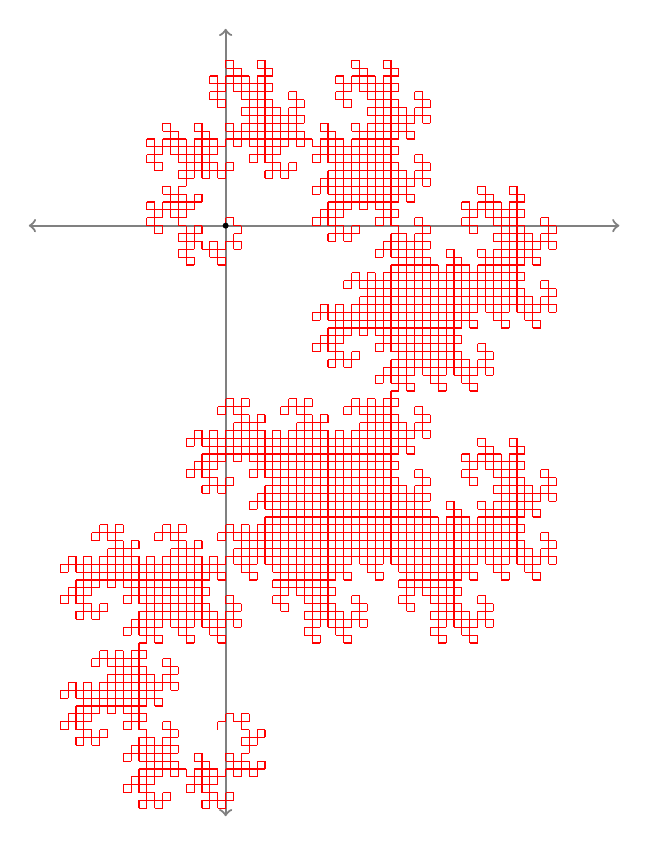
\begin{tikzpicture}[remember picture,scale = 0.1]
\draw[thick, black!50, <->] (-25,0) to (50,0);
\draw[thick, black!50, <->] (0,-75) to (0,25);
\draw[,-,red] (0,0) to (0,1);
\draw[,-,red] (0,1) to (1,1);
\draw[,-,red] (1,1) to (1,0);
\draw[,-,red] (1,0) to (2,0);
\draw[,-,red] (2,0) to (2,-1);
\draw[,-,red] (2,-1) to (1,-1);
\draw[,-,red] (1,-1) to (1,-2);
\draw[,-,red] (1,-2) to (2,-2);
\draw[,-,red] (2,-2) to (2,-3);
\draw[,-,red] (2,-3) to (1,-3);
\draw[,-,red] (1,-3) to (1,-2);
\draw[,-,red] (1,-2) to (0,-2);
\draw[,-,red] (0,-2) to (0,-3);
\draw[,-,red] (0,-3) to (-1,-3);
\draw[,-,red] (-1,-3) to (-1,-4);
\draw[,-,red] (-1,-4) to (0,-4);
\draw[,-,red] (0,-4) to (0,-5);
\draw[,-,red] (0,-5) to (-1,-5);
\draw[,-,red] (-1,-5) to (-1,-4);
\draw[,-,red] (-1,-4) to (-2,-4);
\draw[,-,red] (-2,-4) to (-2,-3);
\draw[,-,red] (-2,-3) to (-1,-3);
\draw[,-,red] (-1,-3) to (-1,-2);
\draw[,-,red] (-1,-2) to (-2,-2);
\draw[,-,red] (-2,-2) to (-2,-3);
\draw[,-,red] (-2,-3) to (-3,-3);
\draw[,-,red] (-3,-3) to (-3,-2);
\draw[,-,red] (-3,-2) to (-4,-2);
\draw[,-,red] (-4,-2) to (-4,-3);
\draw[,-,red] (-4,-3) to (-5,-3);
\draw[,-,red] (-5,-3) to (-5,-4);
\draw[,-,red] (-5,-4) to (-4,-4);
\draw[,-,red] (-4,-4) to (-4,-5);
\draw[,-,red] (-4,-5) to (-5,-5);
\draw[,-,red] (-5,-5) to (-5,-4);
\draw[,-,red] (-5,-4) to (-6,-4);
\draw[,-,red] (-6,-4) to (-6,-3);
\draw[,-,red] (-6,-3) to (-5,-3);
\draw[,-,red] (-5,-3) to (-5,-2);
\draw[,-,red] (-5,-2) to (-6,-2);
\draw[,-,red] (-6,-2) to (-6,-1);
\draw[,-,red] (-6,-1) to (-5,-1);
\draw[,-,red] (-5,-1) to (-5,-2);
\draw[,-,red] (-5,-2) to (-4,-2);
\draw[,-,red] (-4,-2) to (-4,-1);
\draw[,-,red] (-4,-1) to (-3,-1);
\draw[,-,red] (-3,-1) to (-3,0);
\draw[,-,red] (-3,0) to (-4,0);
\draw[,-,red] (-4,0) to (-4,-1);
\draw[,-,red] (-4,-1) to (-5,-1);
\draw[,-,red] (-5,-1) to (-5,0);
\draw[,-,red] (-5,0) to (-6,0);
\draw[,-,red] (-6,0) to (-6,1);
\draw[,-,red] (-6,1) to (-5,1);
\draw[,-,red] (-5,1) to (-5,2);
\draw[,-,red] (-5,2) to (-6,2);
\draw[,-,red] (-6,2) to (-6,1);
\draw[,-,red] (-6,1) to (-7,1);
\draw[,-,red] (-7,1) to (-7,2);
\draw[,-,red] (-7,2) to (-8,2);
\draw[,-,red] (-8,2) to (-8,1);
\draw[,-,red] (-8,1) to (-9,1);
\draw[,-,red] (-9,1) to (-9,0);
\draw[,-,red] (-9,0) to (-8,0);
\draw[,-,red] (-8,0) to (-8,-1);
\draw[,-,red] (-8,-1) to (-9,-1);
\draw[,-,red] (-9,-1) to (-9,0);
\draw[,-,red] (-9,0) to (-10,0);
\draw[,-,red] (-10,0) to (-10,1);
\draw[,-,red] (-10,1) to (-9,1);
\draw[,-,red] (-9,1) to (-9,2);
\draw[,-,red] (-9,2) to (-10,2);
\draw[,-,red] (-10,2) to (-10,3);
\draw[,-,red] (-10,3) to (-9,3);
\draw[,-,red] (-9,3) to (-9,2);
\draw[,-,red] (-9,2) to (-8,2);
\draw[,-,red] (-8,2) to (-8,3);
\draw[,-,red] (-8,3) to (-7,3);
\draw[,-,red] (-7,3) to (-7,4);
\draw[,-,red] (-7,4) to (-8,4);
\draw[,-,red] (-8,4) to (-8,5);
\draw[,-,red] (-8,5) to (-7,5);
\draw[,-,red] (-7,5) to (-7,4);
\draw[,-,red] (-7,4) to (-6,4);
\draw[,-,red] (-6,4) to (-6,3);
\draw[,-,red] (-6,3) to (-7,3);
\draw[,-,red] (-7,3) to (-7,2);
\draw[,-,red] (-7,2) to (-6,2);
\draw[,-,red] (-6,2) to (-6,3);
\draw[,-,red] (-6,3) to (-5,3);
\draw[,-,red] (-5,3) to (-5,2);
\draw[,-,red] (-5,2) to (-4,2);
\draw[,-,red] (-4,2) to (-4,3);
\draw[,-,red] (-4,3) to (-3,3);
\draw[,-,red] (-3,3) to (-3,4);
\draw[,-,red] (-3,4) to (-4,4);
\draw[,-,red] (-4,4) to (-4,3);
\draw[,-,red] (-4,3) to (-5,3);
\draw[,-,red] (-5,3) to (-5,4);
\draw[,-,red] (-5,4) to (-6,4);
\draw[,-,red] (-6,4) to (-6,5);
\draw[,-,red] (-6,5) to (-5,5);
\draw[,-,red] (-5,5) to (-5,6);
\draw[,-,red] (-5,6) to (-6,6);
\draw[,-,red] (-6,6) to (-6,7);
\draw[,-,red] (-6,7) to (-5,7);
\draw[,-,red] (-5,7) to (-5,6);
\draw[,-,red] (-5,6) to (-4,6);
\draw[,-,red] (-4,6) to (-4,7);
\draw[,-,red] (-4,7) to (-3,7);
\draw[,-,red] (-3,7) to (-3,8);
\draw[,-,red] (-3,8) to (-4,8);
\draw[,-,red] (-4,8) to (-4,7);
\draw[,-,red] (-4,7) to (-5,7);
\draw[,-,red] (-5,7) to (-5,8);
\draw[,-,red] (-5,8) to (-6,8);
\draw[,-,red] (-6,8) to (-6,9);
\draw[,-,red] (-6,9) to (-5,9);
\draw[,-,red] (-5,9) to (-5,10);
\draw[,-,red] (-5,10) to (-6,10);
\draw[,-,red] (-6,10) to (-6,9);
\draw[,-,red] (-6,9) to (-7,9);
\draw[,-,red] (-7,9) to (-7,10);
\draw[,-,red] (-7,10) to (-8,10);
\draw[,-,red] (-8,10) to (-8,9);
\draw[,-,red] (-8,9) to (-9,9);
\draw[,-,red] (-9,9) to (-9,8);
\draw[,-,red] (-9,8) to (-8,8);
\draw[,-,red] (-8,8) to (-8,7);
\draw[,-,red] (-8,7) to (-9,7);
\draw[,-,red] (-9,7) to (-9,8);
\draw[,-,red] (-9,8) to (-10,8);
\draw[,-,red] (-10,8) to (-10,9);
\draw[,-,red] (-10,9) to (-9,9);
\draw[,-,red] (-9,9) to (-9,10);
\draw[,-,red] (-9,10) to (-10,10);
\draw[,-,red] (-10,10) to (-10,11);
\draw[,-,red] (-10,11) to (-9,11);
\draw[,-,red] (-9,11) to (-9,10);
\draw[,-,red] (-9,10) to (-8,10);
\draw[,-,red] (-8,10) to (-8,11);
\draw[,-,red] (-8,11) to (-7,11);
\draw[,-,red] (-7,11) to (-7,12);
\draw[,-,red] (-7,12) to (-8,12);
\draw[,-,red] (-8,12) to (-8,13);
\draw[,-,red] (-8,13) to (-7,13);
\draw[,-,red] (-7,13) to (-7,12);
\draw[,-,red] (-7,12) to (-6,12);
\draw[,-,red] (-6,12) to (-6,11);
\draw[,-,red] (-6,11) to (-7,11);
\draw[,-,red] (-7,11) to (-7,10);
\draw[,-,red] (-7,10) to (-6,10);
\draw[,-,red] (-6,10) to (-6,11);
\draw[,-,red] (-6,11) to (-5,11);
\draw[,-,red] (-5,11) to (-5,10);
\draw[,-,red] (-5,10) to (-4,10);
\draw[,-,red] (-4,10) to (-4,11);
\draw[,-,red] (-4,11) to (-3,11);
\draw[,-,red] (-3,11) to (-3,12);
\draw[,-,red] (-3,12) to (-4,12);
\draw[,-,red] (-4,12) to (-4,13);
\draw[,-,red] (-4,13) to (-3,13);
\draw[,-,red] (-3,13) to (-3,12);
\draw[,-,red] (-3,12) to (-2,12);
\draw[,-,red] (-2,12) to (-2,11);
\draw[,-,red] (-2,11) to (-3,11);
\draw[,-,red] (-3,11) to (-3,10);
\draw[,-,red] (-3,10) to (-2,10);
\draw[,-,red] (-2,10) to (-2,9);
\draw[,-,red] (-2,9) to (-3,9);
\draw[,-,red] (-3,9) to (-3,10);
\draw[,-,red] (-3,10) to (-4,10);
\draw[,-,red] (-4,10) to (-4,9);
\draw[,-,red] (-4,9) to (-5,9);
\draw[,-,red] (-5,9) to (-5,8);
\draw[,-,red] (-5,8) to (-4,8);
\draw[,-,red] (-4,8) to (-4,9);
\draw[,-,red] (-4,9) to (-3,9);
\draw[,-,red] (-3,9) to (-3,8);
\draw[,-,red] (-3,8) to (-2,8);
\draw[,-,red] (-2,8) to (-2,7);
\draw[,-,red] (-2,7) to (-3,7);
\draw[,-,red] (-3,7) to (-3,6);
\draw[,-,red] (-3,6) to (-2,6);
\draw[,-,red] (-2,6) to (-2,7);
\draw[,-,red] (-2,7) to (-1,7);
\draw[,-,red] (-1,7) to (-1,6);
\draw[,-,red] (-1,6) to (0,6);
\draw[,-,red] (0,6) to (0,7);
\draw[,-,red] (0,7) to (1,7);
\draw[,-,red] (1,7) to (1,8);
\draw[,-,red] (1,8) to (0,8);
\draw[,-,red] (0,8) to (0,7);
\draw[,-,red] (0,7) to (-1,7);
\draw[,-,red] (-1,7) to (-1,8);
\draw[,-,red] (-1,8) to (-2,8);
\draw[,-,red] (-2,8) to (-2,9);
\draw[,-,red] (-2,9) to (-1,9);
\draw[,-,red] (-1,9) to (-1,10);
\draw[,-,red] (-1,10) to (-2,10);
\draw[,-,red] (-2,10) to (-2,11);
\draw[,-,red] (-2,11) to (-1,11);
\draw[,-,red] (-1,11) to (-1,10);
\draw[,-,red] (-1,10) to (0,10);
\draw[,-,red] (0,10) to (0,11);
\draw[,-,red] (0,11) to (1,11);
\draw[,-,red] (1,11) to (1,12);
\draw[,-,red] (1,12) to (0,12);
\draw[,-,red] (0,12) to (0,13);
\draw[,-,red] (0,13) to (1,13);
\draw[,-,red] (1,13) to (1,12);
\draw[,-,red] (1,12) to (2,12);
\draw[,-,red] (2,12) to (2,11);
\draw[,-,red] (2,11) to (1,11);
\draw[,-,red] (1,11) to (1,10);
\draw[,-,red] (1,10) to (2,10);
\draw[,-,red] (2,10) to (2,11);
\draw[,-,red] (2,11) to (3,11);
\draw[,-,red] (3,11) to (3,10);
\draw[,-,red] (3,10) to (4,10);
\draw[,-,red] (4,10) to (4,11);
\draw[,-,red] (4,11) to (5,11);
\draw[,-,red] (5,11) to (5,12);
\draw[,-,red] (5,12) to (4,12);
\draw[,-,red] (4,12) to (4,11);
\draw[,-,red] (4,11) to (3,11);
\draw[,-,red] (3,11) to (3,12);
\draw[,-,red] (3,12) to (2,12);
\draw[,-,red] (2,12) to (2,13);
\draw[,-,red] (2,13) to (3,13);
\draw[,-,red] (3,13) to (3,14);
\draw[,-,red] (3,14) to (2,14);
\draw[,-,red] (2,14) to (2,15);
\draw[,-,red] (2,15) to (3,15);
\draw[,-,red] (3,15) to (3,14);
\draw[,-,red] (3,14) to (4,14);
\draw[,-,red] (4,14) to (4,15);
\draw[,-,red] (4,15) to (5,15);
\draw[,-,red] (5,15) to (5,16);
\draw[,-,red] (5,16) to (4,16);
\draw[,-,red] (4,16) to (4,15);
\draw[,-,red] (4,15) to (3,15);
\draw[,-,red] (3,15) to (3,16);
\draw[,-,red] (3,16) to (2,16);
\draw[,-,red] (2,16) to (2,17);
\draw[,-,red] (2,17) to (3,17);
\draw[,-,red] (3,17) to (3,18);
\draw[,-,red] (3,18) to (2,18);
\draw[,-,red] (2,18) to (2,17);
\draw[,-,red] (2,17) to (1,17);
\draw[,-,red] (1,17) to (1,18);
\draw[,-,red] (1,18) to (0,18);
\draw[,-,red] (0,18) to (0,17);
\draw[,-,red] (0,17) to (-1,17);
\draw[,-,red] (-1,17) to (-1,16);
\draw[,-,red] (-1,16) to (0,16);
\draw[,-,red] (0,16) to (0,15);
\draw[,-,red] (0,15) to (-1,15);
\draw[,-,red] (-1,15) to (-1,16);
\draw[,-,red] (-1,16) to (-2,16);
\draw[,-,red] (-2,16) to (-2,17);
\draw[,-,red] (-2,17) to (-1,17);
\draw[,-,red] (-1,17) to (-1,18);
\draw[,-,red] (-1,18) to (-2,18);
\draw[,-,red] (-2,18) to (-2,19);
\draw[,-,red] (-2,19) to (-1,19);
\draw[,-,red] (-1,19) to (-1,18);
\draw[,-,red] (-1,18) to (0,18);
\draw[,-,red] (0,18) to (0,19);
\draw[,-,red] (0,19) to (1,19);
\draw[,-,red] (1,19) to (1,20);
\draw[,-,red] (1,20) to (0,20);
\draw[,-,red] (0,20) to (0,21);
\draw[,-,red] (0,21) to (1,21);
\draw[,-,red] (1,21) to (1,20);
\draw[,-,red] (1,20) to (2,20);
\draw[,-,red] (2,20) to (2,19);
\draw[,-,red] (2,19) to (1,19);
\draw[,-,red] (1,19) to (1,18);
\draw[,-,red] (1,18) to (2,18);
\draw[,-,red] (2,18) to (2,19);
\draw[,-,red] (2,19) to (3,19);
\draw[,-,red] (3,19) to (3,18);
\draw[,-,red] (3,18) to (4,18);
\draw[,-,red] (4,18) to (4,19);
\draw[,-,red] (4,19) to (5,19);
\draw[,-,red] (5,19) to (5,20);
\draw[,-,red] (5,20) to (4,20);
\draw[,-,red] (4,20) to (4,21);
\draw[,-,red] (4,21) to (5,21);
\draw[,-,red] (5,21) to (5,20);
\draw[,-,red] (5,20) to (6,20);
\draw[,-,red] (6,20) to (6,19);
\draw[,-,red] (6,19) to (5,19);
\draw[,-,red] (5,19) to (5,18);
\draw[,-,red] (5,18) to (6,18);
\draw[,-,red] (6,18) to (6,17);
\draw[,-,red] (6,17) to (5,17);
\draw[,-,red] (5,17) to (5,18);
\draw[,-,red] (5,18) to (4,18);
\draw[,-,red] (4,18) to (4,17);
\draw[,-,red] (4,17) to (3,17);
\draw[,-,red] (3,17) to (3,16);
\draw[,-,red] (3,16) to (4,16);
\draw[,-,red] (4,16) to (4,17);
\draw[,-,red] (4,17) to (5,17);
\draw[,-,red] (5,17) to (5,16);
\draw[,-,red] (5,16) to (6,16);
\draw[,-,red] (6,16) to (6,15);
\draw[,-,red] (6,15) to (5,15);
\draw[,-,red] (5,15) to (5,14);
\draw[,-,red] (5,14) to (6,14);
\draw[,-,red] (6,14) to (6,15);
\draw[,-,red] (6,15) to (7,15);
\draw[,-,red] (7,15) to (7,14);
\draw[,-,red] (7,14) to (8,14);
\draw[,-,red] (8,14) to (8,15);
\draw[,-,red] (8,15) to (9,15);
\draw[,-,red] (9,15) to (9,16);
\draw[,-,red] (9,16) to (8,16);
\draw[,-,red] (8,16) to (8,17);
\draw[,-,red] (8,17) to (9,17);
\draw[,-,red] (9,17) to (9,16);
\draw[,-,red] (9,16) to (10,16);
\draw[,-,red] (10,16) to (10,15);
\draw[,-,red] (10,15) to (9,15);
\draw[,-,red] (9,15) to (9,14);
\draw[,-,red] (9,14) to (10,14);
\draw[,-,red] (10,14) to (10,13);
\draw[,-,red] (10,13) to (9,13);
\draw[,-,red] (9,13) to (9,14);
\draw[,-,red] (9,14) to (8,14);
\draw[,-,red] (8,14) to (8,13);
\draw[,-,red] (8,13) to (7,13);
\draw[,-,red] (7,13) to (7,12);
\draw[,-,red] (7,12) to (8,12);
\draw[,-,red] (8,12) to (8,11);
\draw[,-,red] (8,11) to (7,11);
\draw[,-,red] (7,11) to (7,12);
\draw[,-,red] (7,12) to (6,12);
\draw[,-,red] (6,12) to (6,13);
\draw[,-,red] (6,13) to (7,13);
\draw[,-,red] (7,13) to (7,14);
\draw[,-,red] (7,14) to (6,14);
\draw[,-,red] (6,14) to (6,13);
\draw[,-,red] (6,13) to (5,13);
\draw[,-,red] (5,13) to (5,14);
\draw[,-,red] (5,14) to (4,14);
\draw[,-,red] (4,14) to (4,13);
\draw[,-,red] (4,13) to (3,13);
\draw[,-,red] (3,13) to (3,12);
\draw[,-,red] (3,12) to (4,12);
\draw[,-,red] (4,12) to (4,13);
\draw[,-,red] (4,13) to (5,13);
\draw[,-,red] (5,13) to (5,12);
\draw[,-,red] (5,12) to (6,12);
\draw[,-,red] (6,12) to (6,11);
\draw[,-,red] (6,11) to (5,11);
\draw[,-,red] (5,11) to (5,10);
\draw[,-,red] (5,10) to (6,10);
\draw[,-,red] (6,10) to (6,9);
\draw[,-,red] (6,9) to (5,9);
\draw[,-,red] (5,9) to (5,10);
\draw[,-,red] (5,10) to (4,10);
\draw[,-,red] (4,10) to (4,9);
\draw[,-,red] (4,9) to (3,9);
\draw[,-,red] (3,9) to (3,8);
\draw[,-,red] (3,8) to (4,8);
\draw[,-,red] (4,8) to (4,9);
\draw[,-,red] (4,9) to (5,9);
\draw[,-,red] (5,9) to (5,8);
\draw[,-,red] (5,8) to (6,8);
\draw[,-,red] (6,8) to (6,7);
\draw[,-,red] (6,7) to (5,7);
\draw[,-,red] (5,7) to (5,6);
\draw[,-,red] (5,6) to (6,6);
\draw[,-,red] (6,6) to (6,7);
\draw[,-,red] (6,7) to (7,7);
\draw[,-,red] (7,7) to (7,6);
\draw[,-,red] (7,6) to (8,6);
\draw[,-,red] (8,6) to (8,7);
\draw[,-,red] (8,7) to (9,7);
\draw[,-,red] (9,7) to (9,8);
\draw[,-,red] (9,8) to (8,8);
\draw[,-,red] (8,8) to (8,7);
\draw[,-,red] (8,7) to (7,7);
\draw[,-,red] (7,7) to (7,8);
\draw[,-,red] (7,8) to (6,8);
\draw[,-,red] (6,8) to (6,9);
\draw[,-,red] (6,9) to (7,9);
\draw[,-,red] (7,9) to (7,10);
\draw[,-,red] (7,10) to (6,10);
\draw[,-,red] (6,10) to (6,11);
\draw[,-,red] (6,11) to (7,11);
\draw[,-,red] (7,11) to (7,10);
\draw[,-,red] (7,10) to (8,10);
\draw[,-,red] (8,10) to (8,11);
\draw[,-,red] (8,11) to (9,11);
\draw[,-,red] (9,11) to (9,12);
\draw[,-,red] (9,12) to (8,12);
\draw[,-,red] (8,12) to (8,13);
\draw[,-,red] (8,13) to (9,13);
\draw[,-,red] (9,13) to (9,12);
\draw[,-,red] (9,12) to (10,12);
\draw[,-,red] (10,12) to (10,11);
\draw[,-,red] (10,11) to (9,11);
\draw[,-,red] (9,11) to (9,10);
\draw[,-,red] (9,10) to (10,10);
\draw[,-,red] (10,10) to (10,11);
\draw[,-,red] (10,11) to (11,11);
\draw[,-,red] (11,11) to (11,10);
\draw[,-,red] (11,10) to (12,10);
\draw[,-,red] (12,10) to (12,11);
\draw[,-,red] (12,11) to (13,11);
\draw[,-,red] (13,11) to (13,12);
\draw[,-,red] (13,12) to (12,12);
\draw[,-,red] (12,12) to (12,13);
\draw[,-,red] (12,13) to (13,13);
\draw[,-,red] (13,13) to (13,12);
\draw[,-,red] (13,12) to (14,12);
\draw[,-,red] (14,12) to (14,11);
\draw[,-,red] (14,11) to (13,11);
\draw[,-,red] (13,11) to (13,10);
\draw[,-,red] (13,10) to (14,10);
\draw[,-,red] (14,10) to (14,9);
\draw[,-,red] (14,9) to (13,9);
\draw[,-,red] (13,9) to (13,10);
\draw[,-,red] (13,10) to (12,10);
\draw[,-,red] (12,10) to (12,9);
\draw[,-,red] (12,9) to (11,9);
\draw[,-,red] (11,9) to (11,8);
\draw[,-,red] (11,8) to (12,8);
\draw[,-,red] (12,8) to (12,9);
\draw[,-,red] (12,9) to (13,9);
\draw[,-,red] (13,9) to (13,8);
\draw[,-,red] (13,8) to (14,8);
\draw[,-,red] (14,8) to (14,7);
\draw[,-,red] (14,7) to (13,7);
\draw[,-,red] (13,7) to (13,6);
\draw[,-,red] (13,6) to (14,6);
\draw[,-,red] (14,6) to (14,7);
\draw[,-,red] (14,7) to (15,7);
\draw[,-,red] (15,7) to (15,6);
\draw[,-,red] (15,6) to (16,6);
\draw[,-,red] (16,6) to (16,7);
\draw[,-,red] (16,7) to (17,7);
\draw[,-,red] (17,7) to (17,8);
\draw[,-,red] (17,8) to (16,8);
\draw[,-,red] (16,8) to (16,7);
\draw[,-,red] (16,7) to (15,7);
\draw[,-,red] (15,7) to (15,8);
\draw[,-,red] (15,8) to (14,8);
\draw[,-,red] (14,8) to (14,9);
\draw[,-,red] (14,9) to (15,9);
\draw[,-,red] (15,9) to (15,10);
\draw[,-,red] (15,10) to (14,10);
\draw[,-,red] (14,10) to (14,11);
\draw[,-,red] (14,11) to (15,11);
\draw[,-,red] (15,11) to (15,10);
\draw[,-,red] (15,10) to (16,10);
\draw[,-,red] (16,10) to (16,11);
\draw[,-,red] (16,11) to (17,11);
\draw[,-,red] (17,11) to (17,12);
\draw[,-,red] (17,12) to (16,12);
\draw[,-,red] (16,12) to (16,13);
\draw[,-,red] (16,13) to (17,13);
\draw[,-,red] (17,13) to (17,12);
\draw[,-,red] (17,12) to (18,12);
\draw[,-,red] (18,12) to (18,11);
\draw[,-,red] (18,11) to (17,11);
\draw[,-,red] (17,11) to (17,10);
\draw[,-,red] (17,10) to (18,10);
\draw[,-,red] (18,10) to (18,11);
\draw[,-,red] (18,11) to (19,11);
\draw[,-,red] (19,11) to (19,10);
\draw[,-,red] (19,10) to (20,10);
\draw[,-,red] (20,10) to (20,11);
\draw[,-,red] (20,11) to (21,11);
\draw[,-,red] (21,11) to (21,12);
\draw[,-,red] (21,12) to (20,12);
\draw[,-,red] (20,12) to (20,11);
\draw[,-,red] (20,11) to (19,11);
\draw[,-,red] (19,11) to (19,12);
\draw[,-,red] (19,12) to (18,12);
\draw[,-,red] (18,12) to (18,13);
\draw[,-,red] (18,13) to (19,13);
\draw[,-,red] (19,13) to (19,14);
\draw[,-,red] (19,14) to (18,14);
\draw[,-,red] (18,14) to (18,15);
\draw[,-,red] (18,15) to (19,15);
\draw[,-,red] (19,15) to (19,14);
\draw[,-,red] (19,14) to (20,14);
\draw[,-,red] (20,14) to (20,15);
\draw[,-,red] (20,15) to (21,15);
\draw[,-,red] (21,15) to (21,16);
\draw[,-,red] (21,16) to (20,16);
\draw[,-,red] (20,16) to (20,15);
\draw[,-,red] (20,15) to (19,15);
\draw[,-,red] (19,15) to (19,16);
\draw[,-,red] (19,16) to (18,16);
\draw[,-,red] (18,16) to (18,17);
\draw[,-,red] (18,17) to (19,17);
\draw[,-,red] (19,17) to (19,18);
\draw[,-,red] (19,18) to (18,18);
\draw[,-,red] (18,18) to (18,17);
\draw[,-,red] (18,17) to (17,17);
\draw[,-,red] (17,17) to (17,18);
\draw[,-,red] (17,18) to (16,18);
\draw[,-,red] (16,18) to (16,17);
\draw[,-,red] (16,17) to (15,17);
\draw[,-,red] (15,17) to (15,16);
\draw[,-,red] (15,16) to (16,16);
\draw[,-,red] (16,16) to (16,15);
\draw[,-,red] (16,15) to (15,15);
\draw[,-,red] (15,15) to (15,16);
\draw[,-,red] (15,16) to (14,16);
\draw[,-,red] (14,16) to (14,17);
\draw[,-,red] (14,17) to (15,17);
\draw[,-,red] (15,17) to (15,18);
\draw[,-,red] (15,18) to (14,18);
\draw[,-,red] (14,18) to (14,19);
\draw[,-,red] (14,19) to (15,19);
\draw[,-,red] (15,19) to (15,18);
\draw[,-,red] (15,18) to (16,18);
\draw[,-,red] (16,18) to (16,19);
\draw[,-,red] (16,19) to (17,19);
\draw[,-,red] (17,19) to (17,20);
\draw[,-,red] (17,20) to (16,20);
\draw[,-,red] (16,20) to (16,21);
\draw[,-,red] (16,21) to (17,21);
\draw[,-,red] (17,21) to (17,20);
\draw[,-,red] (17,20) to (18,20);
\draw[,-,red] (18,20) to (18,19);
\draw[,-,red] (18,19) to (17,19);
\draw[,-,red] (17,19) to (17,18);
\draw[,-,red] (17,18) to (18,18);
\draw[,-,red] (18,18) to (18,19);
\draw[,-,red] (18,19) to (19,19);
\draw[,-,red] (19,19) to (19,18);
\draw[,-,red] (19,18) to (20,18);
\draw[,-,red] (20,18) to (20,19);
\draw[,-,red] (20,19) to (21,19);
\draw[,-,red] (21,19) to (21,20);
\draw[,-,red] (21,20) to (20,20);
\draw[,-,red] (20,20) to (20,21);
\draw[,-,red] (20,21) to (21,21);
\draw[,-,red] (21,21) to (21,20);
\draw[,-,red] (21,20) to (22,20);
\draw[,-,red] (22,20) to (22,19);
\draw[,-,red] (22,19) to (21,19);
\draw[,-,red] (21,19) to (21,18);
\draw[,-,red] (21,18) to (22,18);
\draw[,-,red] (22,18) to (22,17);
\draw[,-,red] (22,17) to (21,17);
\draw[,-,red] (21,17) to (21,18);
\draw[,-,red] (21,18) to (20,18);
\draw[,-,red] (20,18) to (20,17);
\draw[,-,red] (20,17) to (19,17);
\draw[,-,red] (19,17) to (19,16);
\draw[,-,red] (19,16) to (20,16);
\draw[,-,red] (20,16) to (20,17);
\draw[,-,red] (20,17) to (21,17);
\draw[,-,red] (21,17) to (21,16);
\draw[,-,red] (21,16) to (22,16);
\draw[,-,red] (22,16) to (22,15);
\draw[,-,red] (22,15) to (21,15);
\draw[,-,red] (21,15) to (21,14);
\draw[,-,red] (21,14) to (22,14);
\draw[,-,red] (22,14) to (22,15);
\draw[,-,red] (22,15) to (23,15);
\draw[,-,red] (23,15) to (23,14);
\draw[,-,red] (23,14) to (24,14);
\draw[,-,red] (24,14) to (24,15);
\draw[,-,red] (24,15) to (25,15);
\draw[,-,red] (25,15) to (25,16);
\draw[,-,red] (25,16) to (24,16);
\draw[,-,red] (24,16) to (24,17);
\draw[,-,red] (24,17) to (25,17);
\draw[,-,red] (25,17) to (25,16);
\draw[,-,red] (25,16) to (26,16);
\draw[,-,red] (26,16) to (26,15);
\draw[,-,red] (26,15) to (25,15);
\draw[,-,red] (25,15) to (25,14);
\draw[,-,red] (25,14) to (26,14);
\draw[,-,red] (26,14) to (26,13);
\draw[,-,red] (26,13) to (25,13);
\draw[,-,red] (25,13) to (25,14);
\draw[,-,red] (25,14) to (24,14);
\draw[,-,red] (24,14) to (24,13);
\draw[,-,red] (24,13) to (23,13);
\draw[,-,red] (23,13) to (23,12);
\draw[,-,red] (23,12) to (24,12);
\draw[,-,red] (24,12) to (24,11);
\draw[,-,red] (24,11) to (23,11);
\draw[,-,red] (23,11) to (23,12);
\draw[,-,red] (23,12) to (22,12);
\draw[,-,red] (22,12) to (22,13);
\draw[,-,red] (22,13) to (23,13);
\draw[,-,red] (23,13) to (23,14);
\draw[,-,red] (23,14) to (22,14);
\draw[,-,red] (22,14) to (22,13);
\draw[,-,red] (22,13) to (21,13);
\draw[,-,red] (21,13) to (21,14);
\draw[,-,red] (21,14) to (20,14);
\draw[,-,red] (20,14) to (20,13);
\draw[,-,red] (20,13) to (19,13);
\draw[,-,red] (19,13) to (19,12);
\draw[,-,red] (19,12) to (20,12);
\draw[,-,red] (20,12) to (20,13);
\draw[,-,red] (20,13) to (21,13);
\draw[,-,red] (21,13) to (21,12);
\draw[,-,red] (21,12) to (22,12);
\draw[,-,red] (22,12) to (22,11);
\draw[,-,red] (22,11) to (21,11);
\draw[,-,red] (21,11) to (21,10);
\draw[,-,red] (21,10) to (22,10);
\draw[,-,red] (22,10) to (22,9);
\draw[,-,red] (22,9) to (21,9);
\draw[,-,red] (21,9) to (21,10);
\draw[,-,red] (21,10) to (20,10);
\draw[,-,red] (20,10) to (20,9);
\draw[,-,red] (20,9) to (19,9);
\draw[,-,red] (19,9) to (19,8);
\draw[,-,red] (19,8) to (20,8);
\draw[,-,red] (20,8) to (20,9);
\draw[,-,red] (20,9) to (21,9);
\draw[,-,red] (21,9) to (21,8);
\draw[,-,red] (21,8) to (22,8);
\draw[,-,red] (22,8) to (22,7);
\draw[,-,red] (22,7) to (21,7);
\draw[,-,red] (21,7) to (21,6);
\draw[,-,red] (21,6) to (22,6);
\draw[,-,red] (22,6) to (22,7);
\draw[,-,red] (22,7) to (23,7);
\draw[,-,red] (23,7) to (23,6);
\draw[,-,red] (23,6) to (24,6);
\draw[,-,red] (24,6) to (24,7);
\draw[,-,red] (24,7) to (25,7);
\draw[,-,red] (25,7) to (25,8);
\draw[,-,red] (25,8) to (24,8);
\draw[,-,red] (24,8) to (24,9);
\draw[,-,red] (24,9) to (25,9);
\draw[,-,red] (25,9) to (25,8);
\draw[,-,red] (25,8) to (26,8);
\draw[,-,red] (26,8) to (26,7);
\draw[,-,red] (26,7) to (25,7);
\draw[,-,red] (25,7) to (25,6);
\draw[,-,red] (25,6) to (26,6);
\draw[,-,red] (26,6) to (26,5);
\draw[,-,red] (26,5) to (25,5);
\draw[,-,red] (25,5) to (25,6);
\draw[,-,red] (25,6) to (24,6);
\draw[,-,red] (24,6) to (24,5);
\draw[,-,red] (24,5) to (23,5);
\draw[,-,red] (23,5) to (23,4);
\draw[,-,red] (23,4) to (24,4);
\draw[,-,red] (24,4) to (24,3);
\draw[,-,red] (24,3) to (23,3);
\draw[,-,red] (23,3) to (23,4);
\draw[,-,red] (23,4) to (22,4);
\draw[,-,red] (22,4) to (22,5);
\draw[,-,red] (22,5) to (23,5);
\draw[,-,red] (23,5) to (23,6);
\draw[,-,red] (23,6) to (22,6);
\draw[,-,red] (22,6) to (22,5);
\draw[,-,red] (22,5) to (21,5);
\draw[,-,red] (21,5) to (21,6);
\draw[,-,red] (21,6) to (20,6);
\draw[,-,red] (20,6) to (20,5);
\draw[,-,red] (20,5) to (19,5);
\draw[,-,red] (19,5) to (19,4);
\draw[,-,red] (19,4) to (20,4);
\draw[,-,red] (20,4) to (20,3);
\draw[,-,red] (20,3) to (19,3);
\draw[,-,red] (19,3) to (19,4);
\draw[,-,red] (19,4) to (18,4);
\draw[,-,red] (18,4) to (18,5);
\draw[,-,red] (18,5) to (19,5);
\draw[,-,red] (19,5) to (19,6);
\draw[,-,red] (19,6) to (18,6);
\draw[,-,red] (18,6) to (18,7);
\draw[,-,red] (18,7) to (19,7);
\draw[,-,red] (19,7) to (19,6);
\draw[,-,red] (19,6) to (20,6);
\draw[,-,red] (20,6) to (20,7);
\draw[,-,red] (20,7) to (21,7);
\draw[,-,red] (21,7) to (21,8);
\draw[,-,red] (21,8) to (20,8);
\draw[,-,red] (20,8) to (20,7);
\draw[,-,red] (20,7) to (19,7);
\draw[,-,red] (19,7) to (19,8);
\draw[,-,red] (19,8) to (18,8);
\draw[,-,red] (18,8) to (18,9);
\draw[,-,red] (18,9) to (19,9);
\draw[,-,red] (19,9) to (19,10);
\draw[,-,red] (19,10) to (18,10);
\draw[,-,red] (18,10) to (18,9);
\draw[,-,red] (18,9) to (17,9);
\draw[,-,red] (17,9) to (17,10);
\draw[,-,red] (17,10) to (16,10);
\draw[,-,red] (16,10) to (16,9);
\draw[,-,red] (16,9) to (15,9);
\draw[,-,red] (15,9) to (15,8);
\draw[,-,red] (15,8) to (16,8);
\draw[,-,red] (16,8) to (16,9);
\draw[,-,red] (16,9) to (17,9);
\draw[,-,red] (17,9) to (17,8);
\draw[,-,red] (17,8) to (18,8);
\draw[,-,red] (18,8) to (18,7);
\draw[,-,red] (18,7) to (17,7);
\draw[,-,red] (17,7) to (17,6);
\draw[,-,red] (17,6) to (18,6);
\draw[,-,red] (18,6) to (18,5);
\draw[,-,red] (18,5) to (17,5);
\draw[,-,red] (17,5) to (17,6);
\draw[,-,red] (17,6) to (16,6);
\draw[,-,red] (16,6) to (16,5);
\draw[,-,red] (16,5) to (15,5);
\draw[,-,red] (15,5) to (15,4);
\draw[,-,red] (15,4) to (16,4);
\draw[,-,red] (16,4) to (16,3);
\draw[,-,red] (16,3) to (15,3);
\draw[,-,red] (15,3) to (15,4);
\draw[,-,red] (15,4) to (14,4);
\draw[,-,red] (14,4) to (14,5);
\draw[,-,red] (14,5) to (15,5);
\draw[,-,red] (15,5) to (15,6);
\draw[,-,red] (15,6) to (14,6);
\draw[,-,red] (14,6) to (14,5);
\draw[,-,red] (14,5) to (13,5);
\draw[,-,red] (13,5) to (13,6);
\draw[,-,red] (13,6) to (12,6);
\draw[,-,red] (12,6) to (12,5);
\draw[,-,red] (12,5) to (11,5);
\draw[,-,red] (11,5) to (11,4);
\draw[,-,red] (11,4) to (12,4);
\draw[,-,red] (12,4) to (12,5);
\draw[,-,red] (12,5) to (13,5);
\draw[,-,red] (13,5) to (13,4);
\draw[,-,red] (13,4) to (14,4);
\draw[,-,red] (14,4) to (14,3);
\draw[,-,red] (14,3) to (13,3);
\draw[,-,red] (13,3) to (13,2);
\draw[,-,red] (13,2) to (14,2);
\draw[,-,red] (14,2) to (14,1);
\draw[,-,red] (14,1) to (13,1);
\draw[,-,red] (13,1) to (13,2);
\draw[,-,red] (13,2) to (12,2);
\draw[,-,red] (12,2) to (12,1);
\draw[,-,red] (12,1) to (11,1);
\draw[,-,red] (11,1) to (11,0);
\draw[,-,red] (11,0) to (12,0);
\draw[,-,red] (12,0) to (12,1);
\draw[,-,red] (12,1) to (13,1);
\draw[,-,red] (13,1) to (13,0);
\draw[,-,red] (13,0) to (14,0);
\draw[,-,red] (14,0) to (14,-1);
\draw[,-,red] (14,-1) to (13,-1);
\draw[,-,red] (13,-1) to (13,-2);
\draw[,-,red] (13,-2) to (14,-2);
\draw[,-,red] (14,-2) to (14,-1);
\draw[,-,red] (14,-1) to (15,-1);
\draw[,-,red] (15,-1) to (15,-2);
\draw[,-,red] (15,-2) to (16,-2);
\draw[,-,red] (16,-2) to (16,-1);
\draw[,-,red] (16,-1) to (17,-1);
\draw[,-,red] (17,-1) to (17,0);
\draw[,-,red] (17,0) to (16,0);
\draw[,-,red] (16,0) to (16,-1);
\draw[,-,red] (16,-1) to (15,-1);
\draw[,-,red] (15,-1) to (15,0);
\draw[,-,red] (15,0) to (14,0);
\draw[,-,red] (14,0) to (14,1);
\draw[,-,red] (14,1) to (15,1);
\draw[,-,red] (15,1) to (15,2);
\draw[,-,red] (15,2) to (14,2);
\draw[,-,red] (14,2) to (14,3);
\draw[,-,red] (14,3) to (15,3);
\draw[,-,red] (15,3) to (15,2);
\draw[,-,red] (15,2) to (16,2);
\draw[,-,red] (16,2) to (16,3);
\draw[,-,red] (16,3) to (17,3);
\draw[,-,red] (17,3) to (17,4);
\draw[,-,red] (17,4) to (16,4);
\draw[,-,red] (16,4) to (16,5);
\draw[,-,red] (16,5) to (17,5);
\draw[,-,red] (17,5) to (17,4);
\draw[,-,red] (17,4) to (18,4);
\draw[,-,red] (18,4) to (18,3);
\draw[,-,red] (18,3) to (17,3);
\draw[,-,red] (17,3) to (17,2);
\draw[,-,red] (17,2) to (18,2);
\draw[,-,red] (18,2) to (18,3);
\draw[,-,red] (18,3) to (19,3);
\draw[,-,red] (19,3) to (19,2);
\draw[,-,red] (19,2) to (20,2);
\draw[,-,red] (20,2) to (20,3);
\draw[,-,red] (20,3) to (21,3);
\draw[,-,red] (21,3) to (21,4);
\draw[,-,red] (21,4) to (20,4);
\draw[,-,red] (20,4) to (20,5);
\draw[,-,red] (20,5) to (21,5);
\draw[,-,red] (21,5) to (21,4);
\draw[,-,red] (21,4) to (22,4);
\draw[,-,red] (22,4) to (22,3);
\draw[,-,red] (22,3) to (21,3);
\draw[,-,red] (21,3) to (21,2);
\draw[,-,red] (21,2) to (22,2);
\draw[,-,red] (22,2) to (22,1);
\draw[,-,red] (22,1) to (21,1);
\draw[,-,red] (21,1) to (21,2);
\draw[,-,red] (21,2) to (20,2);
\draw[,-,red] (20,2) to (20,1);
\draw[,-,red] (20,1) to (19,1);
\draw[,-,red] (19,1) to (19,0);
\draw[,-,red] (19,0) to (20,0);
\draw[,-,red] (20,0) to (20,1);
\draw[,-,red] (20,1) to (21,1);
\draw[,-,red] (21,1) to (21,0);
\draw[,-,red] (21,0) to (22,0);
\draw[,-,red] (22,0) to (22,-1);
\draw[,-,red] (22,-1) to (21,-1);
\draw[,-,red] (21,-1) to (21,-2);
\draw[,-,red] (21,-2) to (22,-2);
\draw[,-,red] (22,-2) to (22,-1);
\draw[,-,red] (22,-1) to (23,-1);
\draw[,-,red] (23,-1) to (23,-2);
\draw[,-,red] (23,-2) to (24,-2);
\draw[,-,red] (24,-2) to (24,-1);
\draw[,-,red] (24,-1) to (25,-1);
\draw[,-,red] (25,-1) to (25,0);
\draw[,-,red] (25,0) to (24,0);
\draw[,-,red] (24,0) to (24,1);
\draw[,-,red] (24,1) to (25,1);
\draw[,-,red] (25,1) to (25,0);
\draw[,-,red] (25,0) to (26,0);
\draw[,-,red] (26,0) to (26,-1);
\draw[,-,red] (26,-1) to (25,-1);
\draw[,-,red] (25,-1) to (25,-2);
\draw[,-,red] (25,-2) to (26,-2);
\draw[,-,red] (26,-2) to (26,-3);
\draw[,-,red] (26,-3) to (25,-3);
\draw[,-,red] (25,-3) to (25,-2);
\draw[,-,red] (25,-2) to (24,-2);
\draw[,-,red] (24,-2) to (24,-3);
\draw[,-,red] (24,-3) to (23,-3);
\draw[,-,red] (23,-3) to (23,-4);
\draw[,-,red] (23,-4) to (24,-4);
\draw[,-,red] (24,-4) to (24,-5);
\draw[,-,red] (24,-5) to (23,-5);
\draw[,-,red] (23,-5) to (23,-4);
\draw[,-,red] (23,-4) to (22,-4);
\draw[,-,red] (22,-4) to (22,-3);
\draw[,-,red] (22,-3) to (23,-3);
\draw[,-,red] (23,-3) to (23,-2);
\draw[,-,red] (23,-2) to (22,-2);
\draw[,-,red] (22,-2) to (22,-3);
\draw[,-,red] (22,-3) to (21,-3);
\draw[,-,red] (21,-3) to (21,-2);
\draw[,-,red] (21,-2) to (20,-2);
\draw[,-,red] (20,-2) to (20,-3);
\draw[,-,red] (20,-3) to (19,-3);
\draw[,-,red] (19,-3) to (19,-4);
\draw[,-,red] (19,-4) to (20,-4);
\draw[,-,red] (20,-4) to (20,-3);
\draw[,-,red] (20,-3) to (21,-3);
\draw[,-,red] (21,-3) to (21,-4);
\draw[,-,red] (21,-4) to (22,-4);
\draw[,-,red] (22,-4) to (22,-5);
\draw[,-,red] (22,-5) to (21,-5);
\draw[,-,red] (21,-5) to (21,-6);
\draw[,-,red] (21,-6) to (22,-6);
\draw[,-,red] (22,-6) to (22,-7);
\draw[,-,red] (22,-7) to (21,-7);
\draw[,-,red] (21,-7) to (21,-6);
\draw[,-,red] (21,-6) to (20,-6);
\draw[,-,red] (20,-6) to (20,-7);
\draw[,-,red] (20,-7) to (19,-7);
\draw[,-,red] (19,-7) to (19,-8);
\draw[,-,red] (19,-8) to (20,-8);
\draw[,-,red] (20,-8) to (20,-7);
\draw[,-,red] (20,-7) to (21,-7);
\draw[,-,red] (21,-7) to (21,-8);
\draw[,-,red] (21,-8) to (22,-8);
\draw[,-,red] (22,-8) to (22,-9);
\draw[,-,red] (22,-9) to (21,-9);
\draw[,-,red] (21,-9) to (21,-10);
\draw[,-,red] (21,-10) to (22,-10);
\draw[,-,red] (22,-10) to (22,-9);
\draw[,-,red] (22,-9) to (23,-9);
\draw[,-,red] (23,-9) to (23,-10);
\draw[,-,red] (23,-10) to (24,-10);
\draw[,-,red] (24,-10) to (24,-9);
\draw[,-,red] (24,-9) to (25,-9);
\draw[,-,red] (25,-9) to (25,-8);
\draw[,-,red] (25,-8) to (24,-8);
\draw[,-,red] (24,-8) to (24,-9);
\draw[,-,red] (24,-9) to (23,-9);
\draw[,-,red] (23,-9) to (23,-8);
\draw[,-,red] (23,-8) to (22,-8);
\draw[,-,red] (22,-8) to (22,-7);
\draw[,-,red] (22,-7) to (23,-7);
\draw[,-,red] (23,-7) to (23,-6);
\draw[,-,red] (23,-6) to (22,-6);
\draw[,-,red] (22,-6) to (22,-5);
\draw[,-,red] (22,-5) to (23,-5);
\draw[,-,red] (23,-5) to (23,-6);
\draw[,-,red] (23,-6) to (24,-6);
\draw[,-,red] (24,-6) to (24,-5);
\draw[,-,red] (24,-5) to (25,-5);
\draw[,-,red] (25,-5) to (25,-4);
\draw[,-,red] (25,-4) to (24,-4);
\draw[,-,red] (24,-4) to (24,-3);
\draw[,-,red] (24,-3) to (25,-3);
\draw[,-,red] (25,-3) to (25,-4);
\draw[,-,red] (25,-4) to (26,-4);
\draw[,-,red] (26,-4) to (26,-5);
\draw[,-,red] (26,-5) to (25,-5);
\draw[,-,red] (25,-5) to (25,-6);
\draw[,-,red] (25,-6) to (26,-6);
\draw[,-,red] (26,-6) to (26,-5);
\draw[,-,red] (26,-5) to (27,-5);
\draw[,-,red] (27,-5) to (27,-6);
\draw[,-,red] (27,-6) to (28,-6);
\draw[,-,red] (28,-6) to (28,-5);
\draw[,-,red] (28,-5) to (29,-5);
\draw[,-,red] (29,-5) to (29,-4);
\draw[,-,red] (29,-4) to (28,-4);
\draw[,-,red] (28,-4) to (28,-3);
\draw[,-,red] (28,-3) to (29,-3);
\draw[,-,red] (29,-3) to (29,-4);
\draw[,-,red] (29,-4) to (30,-4);
\draw[,-,red] (30,-4) to (30,-5);
\draw[,-,red] (30,-5) to (29,-5);
\draw[,-,red] (29,-5) to (29,-6);
\draw[,-,red] (29,-6) to (30,-6);
\draw[,-,red] (30,-6) to (30,-7);
\draw[,-,red] (30,-7) to (29,-7);
\draw[,-,red] (29,-7) to (29,-6);
\draw[,-,red] (29,-6) to (28,-6);
\draw[,-,red] (28,-6) to (28,-7);
\draw[,-,red] (28,-7) to (27,-7);
\draw[,-,red] (27,-7) to (27,-8);
\draw[,-,red] (27,-8) to (28,-8);
\draw[,-,red] (28,-8) to (28,-7);
\draw[,-,red] (28,-7) to (29,-7);
\draw[,-,red] (29,-7) to (29,-8);
\draw[,-,red] (29,-8) to (30,-8);
\draw[,-,red] (30,-8) to (30,-9);
\draw[,-,red] (30,-9) to (29,-9);
\draw[,-,red] (29,-9) to (29,-10);
\draw[,-,red] (29,-10) to (30,-10);
\draw[,-,red] (30,-10) to (30,-9);
\draw[,-,red] (30,-9) to (31,-9);
\draw[,-,red] (31,-9) to (31,-10);
\draw[,-,red] (31,-10) to (32,-10);
\draw[,-,red] (32,-10) to (32,-9);
\draw[,-,red] (32,-9) to (33,-9);
\draw[,-,red] (33,-9) to (33,-8);
\draw[,-,red] (33,-8) to (32,-8);
\draw[,-,red] (32,-8) to (32,-9);
\draw[,-,red] (32,-9) to (31,-9);
\draw[,-,red] (31,-9) to (31,-8);
\draw[,-,red] (31,-8) to (30,-8);
\draw[,-,red] (30,-8) to (30,-7);
\draw[,-,red] (30,-7) to (31,-7);
\draw[,-,red] (31,-7) to (31,-6);
\draw[,-,red] (31,-6) to (30,-6);
\draw[,-,red] (30,-6) to (30,-5);
\draw[,-,red] (30,-5) to (31,-5);
\draw[,-,red] (31,-5) to (31,-6);
\draw[,-,red] (31,-6) to (32,-6);
\draw[,-,red] (32,-6) to (32,-5);
\draw[,-,red] (32,-5) to (33,-5);
\draw[,-,red] (33,-5) to (33,-4);
\draw[,-,red] (33,-4) to (32,-4);
\draw[,-,red] (32,-4) to (32,-3);
\draw[,-,red] (32,-3) to (33,-3);
\draw[,-,red] (33,-3) to (33,-4);
\draw[,-,red] (33,-4) to (34,-4);
\draw[,-,red] (34,-4) to (34,-5);
\draw[,-,red] (34,-5) to (33,-5);
\draw[,-,red] (33,-5) to (33,-6);
\draw[,-,red] (33,-6) to (34,-6);
\draw[,-,red] (34,-6) to (34,-5);
\draw[,-,red] (34,-5) to (35,-5);
\draw[,-,red] (35,-5) to (35,-6);
\draw[,-,red] (35,-6) to (36,-6);
\draw[,-,red] (36,-6) to (36,-5);
\draw[,-,red] (36,-5) to (37,-5);
\draw[,-,red] (37,-5) to (37,-4);
\draw[,-,red] (37,-4) to (36,-4);
\draw[,-,red] (36,-4) to (36,-5);
\draw[,-,red] (36,-5) to (35,-5);
\draw[,-,red] (35,-5) to (35,-4);
\draw[,-,red] (35,-4) to (34,-4);
\draw[,-,red] (34,-4) to (34,-3);
\draw[,-,red] (34,-3) to (35,-3);
\draw[,-,red] (35,-3) to (35,-2);
\draw[,-,red] (35,-2) to (34,-2);
\draw[,-,red] (34,-2) to (34,-1);
\draw[,-,red] (34,-1) to (35,-1);
\draw[,-,red] (35,-1) to (35,-2);
\draw[,-,red] (35,-2) to (36,-2);
\draw[,-,red] (36,-2) to (36,-1);
\draw[,-,red] (36,-1) to (37,-1);
\draw[,-,red] (37,-1) to (37,0);
\draw[,-,red] (37,0) to (36,0);
\draw[,-,red] (36,0) to (36,-1);
\draw[,-,red] (36,-1) to (35,-1);
\draw[,-,red] (35,-1) to (35,0);
\draw[,-,red] (35,0) to (34,0);
\draw[,-,red] (34,0) to (34,1);
\draw[,-,red] (34,1) to (35,1);
\draw[,-,red] (35,1) to (35,2);
\draw[,-,red] (35,2) to (34,2);
\draw[,-,red] (34,2) to (34,1);
\draw[,-,red] (34,1) to (33,1);
\draw[,-,red] (33,1) to (33,2);
\draw[,-,red] (33,2) to (32,2);
\draw[,-,red] (32,2) to (32,1);
\draw[,-,red] (32,1) to (31,1);
\draw[,-,red] (31,1) to (31,0);
\draw[,-,red] (31,0) to (32,0);
\draw[,-,red] (32,0) to (32,-1);
\draw[,-,red] (32,-1) to (31,-1);
\draw[,-,red] (31,-1) to (31,0);
\draw[,-,red] (31,0) to (30,0);
\draw[,-,red] (30,0) to (30,1);
\draw[,-,red] (30,1) to (31,1);
\draw[,-,red] (31,1) to (31,2);
\draw[,-,red] (31,2) to (30,2);
\draw[,-,red] (30,2) to (30,3);
\draw[,-,red] (30,3) to (31,3);
\draw[,-,red] (31,3) to (31,2);
\draw[,-,red] (31,2) to (32,2);
\draw[,-,red] (32,2) to (32,3);
\draw[,-,red] (32,3) to (33,3);
\draw[,-,red] (33,3) to (33,4);
\draw[,-,red] (33,4) to (32,4);
\draw[,-,red] (32,4) to (32,5);
\draw[,-,red] (32,5) to (33,5);
\draw[,-,red] (33,5) to (33,4);
\draw[,-,red] (33,4) to (34,4);
\draw[,-,red] (34,4) to (34,3);
\draw[,-,red] (34,3) to (33,3);
\draw[,-,red] (33,3) to (33,2);
\draw[,-,red] (33,2) to (34,2);
\draw[,-,red] (34,2) to (34,3);
\draw[,-,red] (34,3) to (35,3);
\draw[,-,red] (35,3) to (35,2);
\draw[,-,red] (35,2) to (36,2);
\draw[,-,red] (36,2) to (36,3);
\draw[,-,red] (36,3) to (37,3);
\draw[,-,red] (37,3) to (37,4);
\draw[,-,red] (37,4) to (36,4);
\draw[,-,red] (36,4) to (36,5);
\draw[,-,red] (36,5) to (37,5);
\draw[,-,red] (37,5) to (37,4);
\draw[,-,red] (37,4) to (38,4);
\draw[,-,red] (38,4) to (38,3);
\draw[,-,red] (38,3) to (37,3);
\draw[,-,red] (37,3) to (37,2);
\draw[,-,red] (37,2) to (38,2);
\draw[,-,red] (38,2) to (38,1);
\draw[,-,red] (38,1) to (37,1);
\draw[,-,red] (37,1) to (37,2);
\draw[,-,red] (37,2) to (36,2);
\draw[,-,red] (36,2) to (36,1);
\draw[,-,red] (36,1) to (35,1);
\draw[,-,red] (35,1) to (35,0);
\draw[,-,red] (35,0) to (36,0);
\draw[,-,red] (36,0) to (36,1);
\draw[,-,red] (36,1) to (37,1);
\draw[,-,red] (37,1) to (37,0);
\draw[,-,red] (37,0) to (38,0);
\draw[,-,red] (38,0) to (38,-1);
\draw[,-,red] (38,-1) to (37,-1);
\draw[,-,red] (37,-1) to (37,-2);
\draw[,-,red] (37,-2) to (38,-2);
\draw[,-,red] (38,-2) to (38,-1);
\draw[,-,red] (38,-1) to (39,-1);
\draw[,-,red] (39,-1) to (39,-2);
\draw[,-,red] (39,-2) to (40,-2);
\draw[,-,red] (40,-2) to (40,-1);
\draw[,-,red] (40,-1) to (41,-1);
\draw[,-,red] (41,-1) to (41,0);
\draw[,-,red] (41,0) to (40,0);
\draw[,-,red] (40,0) to (40,1);
\draw[,-,red] (40,1) to (41,1);
\draw[,-,red] (41,1) to (41,0);
\draw[,-,red] (41,0) to (42,0);
\draw[,-,red] (42,0) to (42,-1);
\draw[,-,red] (42,-1) to (41,-1);
\draw[,-,red] (41,-1) to (41,-2);
\draw[,-,red] (41,-2) to (42,-2);
\draw[,-,red] (42,-2) to (42,-3);
\draw[,-,red] (42,-3) to (41,-3);
\draw[,-,red] (41,-3) to (41,-2);
\draw[,-,red] (41,-2) to (40,-2);
\draw[,-,red] (40,-2) to (40,-3);
\draw[,-,red] (40,-3) to (39,-3);
\draw[,-,red] (39,-3) to (39,-4);
\draw[,-,red] (39,-4) to (40,-4);
\draw[,-,red] (40,-4) to (40,-5);
\draw[,-,red] (40,-5) to (39,-5);
\draw[,-,red] (39,-5) to (39,-4);
\draw[,-,red] (39,-4) to (38,-4);
\draw[,-,red] (38,-4) to (38,-3);
\draw[,-,red] (38,-3) to (39,-3);
\draw[,-,red] (39,-3) to (39,-2);
\draw[,-,red] (39,-2) to (38,-2);
\draw[,-,red] (38,-2) to (38,-3);
\draw[,-,red] (38,-3) to (37,-3);
\draw[,-,red] (37,-3) to (37,-2);
\draw[,-,red] (37,-2) to (36,-2);
\draw[,-,red] (36,-2) to (36,-3);
\draw[,-,red] (36,-3) to (35,-3);
\draw[,-,red] (35,-3) to (35,-4);
\draw[,-,red] (35,-4) to (36,-4);
\draw[,-,red] (36,-4) to (36,-3);
\draw[,-,red] (36,-3) to (37,-3);
\draw[,-,red] (37,-3) to (37,-4);
\draw[,-,red] (37,-4) to (38,-4);
\draw[,-,red] (38,-4) to (38,-5);
\draw[,-,red] (38,-5) to (37,-5);
\draw[,-,red] (37,-5) to (37,-6);
\draw[,-,red] (37,-6) to (38,-6);
\draw[,-,red] (38,-6) to (38,-7);
\draw[,-,red] (38,-7) to (37,-7);
\draw[,-,red] (37,-7) to (37,-6);
\draw[,-,red] (37,-6) to (36,-6);
\draw[,-,red] (36,-6) to (36,-7);
\draw[,-,red] (36,-7) to (35,-7);
\draw[,-,red] (35,-7) to (35,-8);
\draw[,-,red] (35,-8) to (36,-8);
\draw[,-,red] (36,-8) to (36,-7);
\draw[,-,red] (36,-7) to (37,-7);
\draw[,-,red] (37,-7) to (37,-8);
\draw[,-,red] (37,-8) to (38,-8);
\draw[,-,red] (38,-8) to (38,-9);
\draw[,-,red] (38,-9) to (37,-9);
\draw[,-,red] (37,-9) to (37,-10);
\draw[,-,red] (37,-10) to (38,-10);
\draw[,-,red] (38,-10) to (38,-9);
\draw[,-,red] (38,-9) to (39,-9);
\draw[,-,red] (39,-9) to (39,-10);
\draw[,-,red] (39,-10) to (40,-10);
\draw[,-,red] (40,-10) to (40,-9);
\draw[,-,red] (40,-9) to (41,-9);
\draw[,-,red] (41,-9) to (41,-8);
\draw[,-,red] (41,-8) to (40,-8);
\draw[,-,red] (40,-8) to (40,-7);
\draw[,-,red] (40,-7) to (41,-7);
\draw[,-,red] (41,-7) to (41,-8);
\draw[,-,red] (41,-8) to (42,-8);
\draw[,-,red] (42,-8) to (42,-9);
\draw[,-,red] (42,-9) to (41,-9);
\draw[,-,red] (41,-9) to (41,-10);
\draw[,-,red] (41,-10) to (42,-10);
\draw[,-,red] (42,-10) to (42,-11);
\draw[,-,red] (42,-11) to (41,-11);
\draw[,-,red] (41,-11) to (41,-10);
\draw[,-,red] (41,-10) to (40,-10);
\draw[,-,red] (40,-10) to (40,-11);
\draw[,-,red] (40,-11) to (39,-11);
\draw[,-,red] (39,-11) to (39,-12);
\draw[,-,red] (39,-12) to (40,-12);
\draw[,-,red] (40,-12) to (40,-13);
\draw[,-,red] (40,-13) to (39,-13);
\draw[,-,red] (39,-13) to (39,-12);
\draw[,-,red] (39,-12) to (38,-12);
\draw[,-,red] (38,-12) to (38,-11);
\draw[,-,red] (38,-11) to (39,-11);
\draw[,-,red] (39,-11) to (39,-10);
\draw[,-,red] (39,-10) to (38,-10);
\draw[,-,red] (38,-10) to (38,-11);
\draw[,-,red] (38,-11) to (37,-11);
\draw[,-,red] (37,-11) to (37,-10);
\draw[,-,red] (37,-10) to (36,-10);
\draw[,-,red] (36,-10) to (36,-11);
\draw[,-,red] (36,-11) to (35,-11);
\draw[,-,red] (35,-11) to (35,-12);
\draw[,-,red] (35,-12) to (36,-12);
\draw[,-,red] (36,-12) to (36,-13);
\draw[,-,red] (36,-13) to (35,-13);
\draw[,-,red] (35,-13) to (35,-12);
\draw[,-,red] (35,-12) to (34,-12);
\draw[,-,red] (34,-12) to (34,-11);
\draw[,-,red] (34,-11) to (35,-11);
\draw[,-,red] (35,-11) to (35,-10);
\draw[,-,red] (35,-10) to (34,-10);
\draw[,-,red] (34,-10) to (34,-9);
\draw[,-,red] (34,-9) to (35,-9);
\draw[,-,red] (35,-9) to (35,-10);
\draw[,-,red] (35,-10) to (36,-10);
\draw[,-,red] (36,-10) to (36,-9);
\draw[,-,red] (36,-9) to (37,-9);
\draw[,-,red] (37,-9) to (37,-8);
\draw[,-,red] (37,-8) to (36,-8);
\draw[,-,red] (36,-8) to (36,-9);
\draw[,-,red] (36,-9) to (35,-9);
\draw[,-,red] (35,-9) to (35,-8);
\draw[,-,red] (35,-8) to (34,-8);
\draw[,-,red] (34,-8) to (34,-7);
\draw[,-,red] (34,-7) to (35,-7);
\draw[,-,red] (35,-7) to (35,-6);
\draw[,-,red] (35,-6) to (34,-6);
\draw[,-,red] (34,-6) to (34,-7);
\draw[,-,red] (34,-7) to (33,-7);
\draw[,-,red] (33,-7) to (33,-6);
\draw[,-,red] (33,-6) to (32,-6);
\draw[,-,red] (32,-6) to (32,-7);
\draw[,-,red] (32,-7) to (31,-7);
\draw[,-,red] (31,-7) to (31,-8);
\draw[,-,red] (31,-8) to (32,-8);
\draw[,-,red] (32,-8) to (32,-7);
\draw[,-,red] (32,-7) to (33,-7);
\draw[,-,red] (33,-7) to (33,-8);
\draw[,-,red] (33,-8) to (34,-8);
\draw[,-,red] (34,-8) to (34,-9);
\draw[,-,red] (34,-9) to (33,-9);
\draw[,-,red] (33,-9) to (33,-10);
\draw[,-,red] (33,-10) to (34,-10);
\draw[,-,red] (34,-10) to (34,-11);
\draw[,-,red] (34,-11) to (33,-11);
\draw[,-,red] (33,-11) to (33,-10);
\draw[,-,red] (33,-10) to (32,-10);
\draw[,-,red] (32,-10) to (32,-11);
\draw[,-,red] (32,-11) to (31,-11);
\draw[,-,red] (31,-11) to (31,-12);
\draw[,-,red] (31,-12) to (32,-12);
\draw[,-,red] (32,-12) to (32,-13);
\draw[,-,red] (32,-13) to (31,-13);
\draw[,-,red] (31,-13) to (31,-12);
\draw[,-,red] (31,-12) to (30,-12);
\draw[,-,red] (30,-12) to (30,-11);
\draw[,-,red] (30,-11) to (31,-11);
\draw[,-,red] (31,-11) to (31,-10);
\draw[,-,red] (31,-10) to (30,-10);
\draw[,-,red] (30,-10) to (30,-11);
\draw[,-,red] (30,-11) to (29,-11);
\draw[,-,red] (29,-11) to (29,-10);
\draw[,-,red] (29,-10) to (28,-10);
\draw[,-,red] (28,-10) to (28,-11);
\draw[,-,red] (28,-11) to (27,-11);
\draw[,-,red] (27,-11) to (27,-12);
\draw[,-,red] (27,-12) to (28,-12);
\draw[,-,red] (28,-12) to (28,-11);
\draw[,-,red] (28,-11) to (29,-11);
\draw[,-,red] (29,-11) to (29,-12);
\draw[,-,red] (29,-12) to (30,-12);
\draw[,-,red] (30,-12) to (30,-13);
\draw[,-,red] (30,-13) to (29,-13);
\draw[,-,red] (29,-13) to (29,-14);
\draw[,-,red] (29,-14) to (30,-14);
\draw[,-,red] (30,-14) to (30,-15);
\draw[,-,red] (30,-15) to (29,-15);
\draw[,-,red] (29,-15) to (29,-14);
\draw[,-,red] (29,-14) to (28,-14);
\draw[,-,red] (28,-14) to (28,-15);
\draw[,-,red] (28,-15) to (27,-15);
\draw[,-,red] (27,-15) to (27,-16);
\draw[,-,red] (27,-16) to (28,-16);
\draw[,-,red] (28,-16) to (28,-15);
\draw[,-,red] (28,-15) to (29,-15);
\draw[,-,red] (29,-15) to (29,-16);
\draw[,-,red] (29,-16) to (30,-16);
\draw[,-,red] (30,-16) to (30,-17);
\draw[,-,red] (30,-17) to (29,-17);
\draw[,-,red] (29,-17) to (29,-18);
\draw[,-,red] (29,-18) to (30,-18);
\draw[,-,red] (30,-18) to (30,-17);
\draw[,-,red] (30,-17) to (31,-17);
\draw[,-,red] (31,-17) to (31,-18);
\draw[,-,red] (31,-18) to (32,-18);
\draw[,-,red] (32,-18) to (32,-17);
\draw[,-,red] (32,-17) to (33,-17);
\draw[,-,red] (33,-17) to (33,-16);
\draw[,-,red] (33,-16) to (32,-16);
\draw[,-,red] (32,-16) to (32,-15);
\draw[,-,red] (32,-15) to (33,-15);
\draw[,-,red] (33,-15) to (33,-16);
\draw[,-,red] (33,-16) to (34,-16);
\draw[,-,red] (34,-16) to (34,-17);
\draw[,-,red] (34,-17) to (33,-17);
\draw[,-,red] (33,-17) to (33,-18);
\draw[,-,red] (33,-18) to (34,-18);
\draw[,-,red] (34,-18) to (34,-19);
\draw[,-,red] (34,-19) to (33,-19);
\draw[,-,red] (33,-19) to (33,-18);
\draw[,-,red] (33,-18) to (32,-18);
\draw[,-,red] (32,-18) to (32,-19);
\draw[,-,red] (32,-19) to (31,-19);
\draw[,-,red] (31,-19) to (31,-20);
\draw[,-,red] (31,-20) to (32,-20);
\draw[,-,red] (32,-20) to (32,-21);
\draw[,-,red] (32,-21) to (31,-21);
\draw[,-,red] (31,-21) to (31,-20);
\draw[,-,red] (31,-20) to (30,-20);
\draw[,-,red] (30,-20) to (30,-19);
\draw[,-,red] (30,-19) to (31,-19);
\draw[,-,red] (31,-19) to (31,-18);
\draw[,-,red] (31,-18) to (30,-18);
\draw[,-,red] (30,-18) to (30,-19);
\draw[,-,red] (30,-19) to (29,-19);
\draw[,-,red] (29,-19) to (29,-18);
\draw[,-,red] (29,-18) to (28,-18);
\draw[,-,red] (28,-18) to (28,-19);
\draw[,-,red] (28,-19) to (27,-19);
\draw[,-,red] (27,-19) to (27,-20);
\draw[,-,red] (27,-20) to (28,-20);
\draw[,-,red] (28,-20) to (28,-21);
\draw[,-,red] (28,-21) to (27,-21);
\draw[,-,red] (27,-21) to (27,-20);
\draw[,-,red] (27,-20) to (26,-20);
\draw[,-,red] (26,-20) to (26,-19);
\draw[,-,red] (26,-19) to (27,-19);
\draw[,-,red] (27,-19) to (27,-18);
\draw[,-,red] (27,-18) to (26,-18);
\draw[,-,red] (26,-18) to (26,-17);
\draw[,-,red] (26,-17) to (27,-17);
\draw[,-,red] (27,-17) to (27,-18);
\draw[,-,red] (27,-18) to (28,-18);
\draw[,-,red] (28,-18) to (28,-17);
\draw[,-,red] (28,-17) to (29,-17);
\draw[,-,red] (29,-17) to (29,-16);
\draw[,-,red] (29,-16) to (28,-16);
\draw[,-,red] (28,-16) to (28,-17);
\draw[,-,red] (28,-17) to (27,-17);
\draw[,-,red] (27,-17) to (27,-16);
\draw[,-,red] (27,-16) to (26,-16);
\draw[,-,red] (26,-16) to (26,-15);
\draw[,-,red] (26,-15) to (27,-15);
\draw[,-,red] (27,-15) to (27,-14);
\draw[,-,red] (27,-14) to (26,-14);
\draw[,-,red] (26,-14) to (26,-15);
\draw[,-,red] (26,-15) to (25,-15);
\draw[,-,red] (25,-15) to (25,-14);
\draw[,-,red] (25,-14) to (24,-14);
\draw[,-,red] (24,-14) to (24,-15);
\draw[,-,red] (24,-15) to (23,-15);
\draw[,-,red] (23,-15) to (23,-16);
\draw[,-,red] (23,-16) to (24,-16);
\draw[,-,red] (24,-16) to (24,-17);
\draw[,-,red] (24,-17) to (23,-17);
\draw[,-,red] (23,-17) to (23,-16);
\draw[,-,red] (23,-16) to (22,-16);
\draw[,-,red] (22,-16) to (22,-15);
\draw[,-,red] (22,-15) to (23,-15);
\draw[,-,red] (23,-15) to (23,-14);
\draw[,-,red] (23,-14) to (22,-14);
\draw[,-,red] (22,-14) to (22,-13);
\draw[,-,red] (22,-13) to (23,-13);
\draw[,-,red] (23,-13) to (23,-14);
\draw[,-,red] (23,-14) to (24,-14);
\draw[,-,red] (24,-14) to (24,-13);
\draw[,-,red] (24,-13) to (25,-13);
\draw[,-,red] (25,-13) to (25,-12);
\draw[,-,red] (25,-12) to (24,-12);
\draw[,-,red] (24,-12) to (24,-11);
\draw[,-,red] (24,-11) to (25,-11);
\draw[,-,red] (25,-11) to (25,-12);
\draw[,-,red] (25,-12) to (26,-12);
\draw[,-,red] (26,-12) to (26,-13);
\draw[,-,red] (26,-13) to (25,-13);
\draw[,-,red] (25,-13) to (25,-14);
\draw[,-,red] (25,-14) to (26,-14);
\draw[,-,red] (26,-14) to (26,-13);
\draw[,-,red] (26,-13) to (27,-13);
\draw[,-,red] (27,-13) to (27,-14);
\draw[,-,red] (27,-14) to (28,-14);
\draw[,-,red] (28,-14) to (28,-13);
\draw[,-,red] (28,-13) to (29,-13);
\draw[,-,red] (29,-13) to (29,-12);
\draw[,-,red] (29,-12) to (28,-12);
\draw[,-,red] (28,-12) to (28,-13);
\draw[,-,red] (28,-13) to (27,-13);
\draw[,-,red] (27,-13) to (27,-12);
\draw[,-,red] (27,-12) to (26,-12);
\draw[,-,red] (26,-12) to (26,-11);
\draw[,-,red] (26,-11) to (27,-11);
\draw[,-,red] (27,-11) to (27,-10);
\draw[,-,red] (27,-10) to (26,-10);
\draw[,-,red] (26,-10) to (26,-9);
\draw[,-,red] (26,-9) to (27,-9);
\draw[,-,red] (27,-9) to (27,-10);
\draw[,-,red] (27,-10) to (28,-10);
\draw[,-,red] (28,-10) to (28,-9);
\draw[,-,red] (28,-9) to (29,-9);
\draw[,-,red] (29,-9) to (29,-8);
\draw[,-,red] (29,-8) to (28,-8);
\draw[,-,red] (28,-8) to (28,-9);
\draw[,-,red] (28,-9) to (27,-9);
\draw[,-,red] (27,-9) to (27,-8);
\draw[,-,red] (27,-8) to (26,-8);
\draw[,-,red] (26,-8) to (26,-7);
\draw[,-,red] (26,-7) to (27,-7);
\draw[,-,red] (27,-7) to (27,-6);
\draw[,-,red] (27,-6) to (26,-6);
\draw[,-,red] (26,-6) to (26,-7);
\draw[,-,red] (26,-7) to (25,-7);
\draw[,-,red] (25,-7) to (25,-6);
\draw[,-,red] (25,-6) to (24,-6);
\draw[,-,red] (24,-6) to (24,-7);
\draw[,-,red] (24,-7) to (23,-7);
\draw[,-,red] (23,-7) to (23,-8);
\draw[,-,red] (23,-8) to (24,-8);
\draw[,-,red] (24,-8) to (24,-7);
\draw[,-,red] (24,-7) to (25,-7);
\draw[,-,red] (25,-7) to (25,-8);
\draw[,-,red] (25,-8) to (26,-8);
\draw[,-,red] (26,-8) to (26,-9);
\draw[,-,red] (26,-9) to (25,-9);
\draw[,-,red] (25,-9) to (25,-10);
\draw[,-,red] (25,-10) to (26,-10);
\draw[,-,red] (26,-10) to (26,-11);
\draw[,-,red] (26,-11) to (25,-11);
\draw[,-,red] (25,-11) to (25,-10);
\draw[,-,red] (25,-10) to (24,-10);
\draw[,-,red] (24,-10) to (24,-11);
\draw[,-,red] (24,-11) to (23,-11);
\draw[,-,red] (23,-11) to (23,-12);
\draw[,-,red] (23,-12) to (24,-12);
\draw[,-,red] (24,-12) to (24,-13);
\draw[,-,red] (24,-13) to (23,-13);
\draw[,-,red] (23,-13) to (23,-12);
\draw[,-,red] (23,-12) to (22,-12);
\draw[,-,red] (22,-12) to (22,-11);
\draw[,-,red] (22,-11) to (23,-11);
\draw[,-,red] (23,-11) to (23,-10);
\draw[,-,red] (23,-10) to (22,-10);
\draw[,-,red] (22,-10) to (22,-11);
\draw[,-,red] (22,-11) to (21,-11);
\draw[,-,red] (21,-11) to (21,-10);
\draw[,-,red] (21,-10) to (20,-10);
\draw[,-,red] (20,-10) to (20,-11);
\draw[,-,red] (20,-11) to (19,-11);
\draw[,-,red] (19,-11) to (19,-12);
\draw[,-,red] (19,-12) to (20,-12);
\draw[,-,red] (20,-12) to (20,-13);
\draw[,-,red] (20,-13) to (19,-13);
\draw[,-,red] (19,-13) to (19,-12);
\draw[,-,red] (19,-12) to (18,-12);
\draw[,-,red] (18,-12) to (18,-11);
\draw[,-,red] (18,-11) to (19,-11);
\draw[,-,red] (19,-11) to (19,-10);
\draw[,-,red] (19,-10) to (18,-10);
\draw[,-,red] (18,-10) to (18,-9);
\draw[,-,red] (18,-9) to (19,-9);
\draw[,-,red] (19,-9) to (19,-10);
\draw[,-,red] (19,-10) to (20,-10);
\draw[,-,red] (20,-10) to (20,-9);
\draw[,-,red] (20,-9) to (21,-9);
\draw[,-,red] (21,-9) to (21,-8);
\draw[,-,red] (21,-8) to (20,-8);
\draw[,-,red] (20,-8) to (20,-9);
\draw[,-,red] (20,-9) to (19,-9);
\draw[,-,red] (19,-9) to (19,-8);
\draw[,-,red] (19,-8) to (18,-8);
\draw[,-,red] (18,-8) to (18,-7);
\draw[,-,red] (18,-7) to (19,-7);
\draw[,-,red] (19,-7) to (19,-6);
\draw[,-,red] (19,-6) to (18,-6);
\draw[,-,red] (18,-6) to (18,-7);
\draw[,-,red] (18,-7) to (17,-7);
\draw[,-,red] (17,-7) to (17,-6);
\draw[,-,red] (17,-6) to (16,-6);
\draw[,-,red] (16,-6) to (16,-7);
\draw[,-,red] (16,-7) to (15,-7);
\draw[,-,red] (15,-7) to (15,-8);
\draw[,-,red] (15,-8) to (16,-8);
\draw[,-,red] (16,-8) to (16,-7);
\draw[,-,red] (16,-7) to (17,-7);
\draw[,-,red] (17,-7) to (17,-8);
\draw[,-,red] (17,-8) to (18,-8);
\draw[,-,red] (18,-8) to (18,-9);
\draw[,-,red] (18,-9) to (17,-9);
\draw[,-,red] (17,-9) to (17,-10);
\draw[,-,red] (17,-10) to (18,-10);
\draw[,-,red] (18,-10) to (18,-11);
\draw[,-,red] (18,-11) to (17,-11);
\draw[,-,red] (17,-11) to (17,-10);
\draw[,-,red] (17,-10) to (16,-10);
\draw[,-,red] (16,-10) to (16,-11);
\draw[,-,red] (16,-11) to (15,-11);
\draw[,-,red] (15,-11) to (15,-12);
\draw[,-,red] (15,-12) to (16,-12);
\draw[,-,red] (16,-12) to (16,-13);
\draw[,-,red] (16,-13) to (15,-13);
\draw[,-,red] (15,-13) to (15,-12);
\draw[,-,red] (15,-12) to (14,-12);
\draw[,-,red] (14,-12) to (14,-11);
\draw[,-,red] (14,-11) to (15,-11);
\draw[,-,red] (15,-11) to (15,-10);
\draw[,-,red] (15,-10) to (14,-10);
\draw[,-,red] (14,-10) to (14,-11);
\draw[,-,red] (14,-11) to (13,-11);
\draw[,-,red] (13,-11) to (13,-10);
\draw[,-,red] (13,-10) to (12,-10);
\draw[,-,red] (12,-10) to (12,-11);
\draw[,-,red] (12,-11) to (11,-11);
\draw[,-,red] (11,-11) to (11,-12);
\draw[,-,red] (11,-12) to (12,-12);
\draw[,-,red] (12,-12) to (12,-11);
\draw[,-,red] (12,-11) to (13,-11);
\draw[,-,red] (13,-11) to (13,-12);
\draw[,-,red] (13,-12) to (14,-12);
\draw[,-,red] (14,-12) to (14,-13);
\draw[,-,red] (14,-13) to (13,-13);
\draw[,-,red] (13,-13) to (13,-14);
\draw[,-,red] (13,-14) to (14,-14);
\draw[,-,red] (14,-14) to (14,-15);
\draw[,-,red] (14,-15) to (13,-15);
\draw[,-,red] (13,-15) to (13,-14);
\draw[,-,red] (13,-14) to (12,-14);
\draw[,-,red] (12,-14) to (12,-15);
\draw[,-,red] (12,-15) to (11,-15);
\draw[,-,red] (11,-15) to (11,-16);
\draw[,-,red] (11,-16) to (12,-16);
\draw[,-,red] (12,-16) to (12,-15);
\draw[,-,red] (12,-15) to (13,-15);
\draw[,-,red] (13,-15) to (13,-16);
\draw[,-,red] (13,-16) to (14,-16);
\draw[,-,red] (14,-16) to (14,-17);
\draw[,-,red] (14,-17) to (13,-17);
\draw[,-,red] (13,-17) to (13,-18);
\draw[,-,red] (13,-18) to (14,-18);
\draw[,-,red] (14,-18) to (14,-17);
\draw[,-,red] (14,-17) to (15,-17);
\draw[,-,red] (15,-17) to (15,-18);
\draw[,-,red] (15,-18) to (16,-18);
\draw[,-,red] (16,-18) to (16,-17);
\draw[,-,red] (16,-17) to (17,-17);
\draw[,-,red] (17,-17) to (17,-16);
\draw[,-,red] (17,-16) to (16,-16);
\draw[,-,red] (16,-16) to (16,-17);
\draw[,-,red] (16,-17) to (15,-17);
\draw[,-,red] (15,-17) to (15,-16);
\draw[,-,red] (15,-16) to (14,-16);
\draw[,-,red] (14,-16) to (14,-15);
\draw[,-,red] (14,-15) to (15,-15);
\draw[,-,red] (15,-15) to (15,-14);
\draw[,-,red] (15,-14) to (14,-14);
\draw[,-,red] (14,-14) to (14,-13);
\draw[,-,red] (14,-13) to (15,-13);
\draw[,-,red] (15,-13) to (15,-14);
\draw[,-,red] (15,-14) to (16,-14);
\draw[,-,red] (16,-14) to (16,-13);
\draw[,-,red] (16,-13) to (17,-13);
\draw[,-,red] (17,-13) to (17,-12);
\draw[,-,red] (17,-12) to (16,-12);
\draw[,-,red] (16,-12) to (16,-11);
\draw[,-,red] (16,-11) to (17,-11);
\draw[,-,red] (17,-11) to (17,-12);
\draw[,-,red] (17,-12) to (18,-12);
\draw[,-,red] (18,-12) to (18,-13);
\draw[,-,red] (18,-13) to (17,-13);
\draw[,-,red] (17,-13) to (17,-14);
\draw[,-,red] (17,-14) to (18,-14);
\draw[,-,red] (18,-14) to (18,-13);
\draw[,-,red] (18,-13) to (19,-13);
\draw[,-,red] (19,-13) to (19,-14);
\draw[,-,red] (19,-14) to (20,-14);
\draw[,-,red] (20,-14) to (20,-13);
\draw[,-,red] (20,-13) to (21,-13);
\draw[,-,red] (21,-13) to (21,-12);
\draw[,-,red] (21,-12) to (20,-12);
\draw[,-,red] (20,-12) to (20,-11);
\draw[,-,red] (20,-11) to (21,-11);
\draw[,-,red] (21,-11) to (21,-12);
\draw[,-,red] (21,-12) to (22,-12);
\draw[,-,red] (22,-12) to (22,-13);
\draw[,-,red] (22,-13) to (21,-13);
\draw[,-,red] (21,-13) to (21,-14);
\draw[,-,red] (21,-14) to (22,-14);
\draw[,-,red] (22,-14) to (22,-15);
\draw[,-,red] (22,-15) to (21,-15);
\draw[,-,red] (21,-15) to (21,-14);
\draw[,-,red] (21,-14) to (20,-14);
\draw[,-,red] (20,-14) to (20,-15);
\draw[,-,red] (20,-15) to (19,-15);
\draw[,-,red] (19,-15) to (19,-16);
\draw[,-,red] (19,-16) to (20,-16);
\draw[,-,red] (20,-16) to (20,-15);
\draw[,-,red] (20,-15) to (21,-15);
\draw[,-,red] (21,-15) to (21,-16);
\draw[,-,red] (21,-16) to (22,-16);
\draw[,-,red] (22,-16) to (22,-17);
\draw[,-,red] (22,-17) to (21,-17);
\draw[,-,red] (21,-17) to (21,-18);
\draw[,-,red] (21,-18) to (22,-18);
\draw[,-,red] (22,-18) to (22,-17);
\draw[,-,red] (22,-17) to (23,-17);
\draw[,-,red] (23,-17) to (23,-18);
\draw[,-,red] (23,-18) to (24,-18);
\draw[,-,red] (24,-18) to (24,-17);
\draw[,-,red] (24,-17) to (25,-17);
\draw[,-,red] (25,-17) to (25,-16);
\draw[,-,red] (25,-16) to (24,-16);
\draw[,-,red] (24,-16) to (24,-15);
\draw[,-,red] (24,-15) to (25,-15);
\draw[,-,red] (25,-15) to (25,-16);
\draw[,-,red] (25,-16) to (26,-16);
\draw[,-,red] (26,-16) to (26,-17);
\draw[,-,red] (26,-17) to (25,-17);
\draw[,-,red] (25,-17) to (25,-18);
\draw[,-,red] (25,-18) to (26,-18);
\draw[,-,red] (26,-18) to (26,-19);
\draw[,-,red] (26,-19) to (25,-19);
\draw[,-,red] (25,-19) to (25,-18);
\draw[,-,red] (25,-18) to (24,-18);
\draw[,-,red] (24,-18) to (24,-19);
\draw[,-,red] (24,-19) to (23,-19);
\draw[,-,red] (23,-19) to (23,-20);
\draw[,-,red] (23,-20) to (24,-20);
\draw[,-,red] (24,-20) to (24,-21);
\draw[,-,red] (24,-21) to (23,-21);
\draw[,-,red] (23,-21) to (23,-20);
\draw[,-,red] (23,-20) to (22,-20);
\draw[,-,red] (22,-20) to (22,-19);
\draw[,-,red] (22,-19) to (23,-19);
\draw[,-,red] (23,-19) to (23,-18);
\draw[,-,red] (23,-18) to (22,-18);
\draw[,-,red] (22,-18) to (22,-19);
\draw[,-,red] (22,-19) to (21,-19);
\draw[,-,red] (21,-19) to (21,-18);
\draw[,-,red] (21,-18) to (20,-18);
\draw[,-,red] (20,-18) to (20,-19);
\draw[,-,red] (20,-19) to (19,-19);
\draw[,-,red] (19,-19) to (19,-20);
\draw[,-,red] (19,-20) to (20,-20);
\draw[,-,red] (20,-20) to (20,-19);
\draw[,-,red] (20,-19) to (21,-19);
\draw[,-,red] (21,-19) to (21,-20);
\draw[,-,red] (21,-20) to (22,-20);
\draw[,-,red] (22,-20) to (22,-21);
\draw[,-,red] (22,-21) to (21,-21);
\draw[,-,red] (21,-21) to (21,-22);
\draw[,-,red] (21,-22) to (22,-22);
\draw[,-,red] (22,-22) to (22,-23);
\draw[,-,red] (22,-23) to (21,-23);
\draw[,-,red] (21,-23) to (21,-22);
\draw[,-,red] (21,-22) to (20,-22);
\draw[,-,red] (20,-22) to (20,-23);
\draw[,-,red] (20,-23) to (19,-23);
\draw[,-,red] (19,-23) to (19,-24);
\draw[,-,red] (19,-24) to (20,-24);
\draw[,-,red] (20,-24) to (20,-23);
\draw[,-,red] (20,-23) to (21,-23);
\draw[,-,red] (21,-23) to (21,-24);
\draw[,-,red] (21,-24) to (22,-24);
\draw[,-,red] (22,-24) to (22,-25);
\draw[,-,red] (22,-25) to (21,-25);
\draw[,-,red] (21,-25) to (21,-26);
\draw[,-,red] (21,-26) to (22,-26);
\draw[,-,red] (22,-26) to (22,-25);
\draw[,-,red] (22,-25) to (23,-25);
\draw[,-,red] (23,-25) to (23,-26);
\draw[,-,red] (23,-26) to (24,-26);
\draw[,-,red] (24,-26) to (24,-25);
\draw[,-,red] (24,-25) to (25,-25);
\draw[,-,red] (25,-25) to (25,-24);
\draw[,-,red] (25,-24) to (24,-24);
\draw[,-,red] (24,-24) to (24,-23);
\draw[,-,red] (24,-23) to (25,-23);
\draw[,-,red] (25,-23) to (25,-24);
\draw[,-,red] (25,-24) to (26,-24);
\draw[,-,red] (26,-24) to (26,-25);
\draw[,-,red] (26,-25) to (25,-25);
\draw[,-,red] (25,-25) to (25,-26);
\draw[,-,red] (25,-26) to (26,-26);
\draw[,-,red] (26,-26) to (26,-27);
\draw[,-,red] (26,-27) to (25,-27);
\draw[,-,red] (25,-27) to (25,-26);
\draw[,-,red] (25,-26) to (24,-26);
\draw[,-,red] (24,-26) to (24,-27);
\draw[,-,red] (24,-27) to (23,-27);
\draw[,-,red] (23,-27) to (23,-28);
\draw[,-,red] (23,-28) to (24,-28);
\draw[,-,red] (24,-28) to (24,-29);
\draw[,-,red] (24,-29) to (23,-29);
\draw[,-,red] (23,-29) to (23,-28);
\draw[,-,red] (23,-28) to (22,-28);
\draw[,-,red] (22,-28) to (22,-27);
\draw[,-,red] (22,-27) to (23,-27);
\draw[,-,red] (23,-27) to (23,-26);
\draw[,-,red] (23,-26) to (22,-26);
\draw[,-,red] (22,-26) to (22,-27);
\draw[,-,red] (22,-27) to (21,-27);
\draw[,-,red] (21,-27) to (21,-26);
\draw[,-,red] (21,-26) to (20,-26);
\draw[,-,red] (20,-26) to (20,-27);
\draw[,-,red] (20,-27) to (19,-27);
\draw[,-,red] (19,-27) to (19,-28);
\draw[,-,red] (19,-28) to (20,-28);
\draw[,-,red] (20,-28) to (20,-29);
\draw[,-,red] (20,-29) to (19,-29);
\draw[,-,red] (19,-29) to (19,-28);
\draw[,-,red] (19,-28) to (18,-28);
\draw[,-,red] (18,-28) to (18,-27);
\draw[,-,red] (18,-27) to (19,-27);
\draw[,-,red] (19,-27) to (19,-26);
\draw[,-,red] (19,-26) to (18,-26);
\draw[,-,red] (18,-26) to (18,-25);
\draw[,-,red] (18,-25) to (19,-25);
\draw[,-,red] (19,-25) to (19,-26);
\draw[,-,red] (19,-26) to (20,-26);
\draw[,-,red] (20,-26) to (20,-25);
\draw[,-,red] (20,-25) to (21,-25);
\draw[,-,red] (21,-25) to (21,-24);
\draw[,-,red] (21,-24) to (20,-24);
\draw[,-,red] (20,-24) to (20,-25);
\draw[,-,red] (20,-25) to (19,-25);
\draw[,-,red] (19,-25) to (19,-24);
\draw[,-,red] (19,-24) to (18,-24);
\draw[,-,red] (18,-24) to (18,-23);
\draw[,-,red] (18,-23) to (19,-23);
\draw[,-,red] (19,-23) to (19,-22);
\draw[,-,red] (19,-22) to (18,-22);
\draw[,-,red] (18,-22) to (18,-23);
\draw[,-,red] (18,-23) to (17,-23);
\draw[,-,red] (17,-23) to (17,-22);
\draw[,-,red] (17,-22) to (16,-22);
\draw[,-,red] (16,-22) to (16,-23);
\draw[,-,red] (16,-23) to (15,-23);
\draw[,-,red] (15,-23) to (15,-24);
\draw[,-,red] (15,-24) to (16,-24);
\draw[,-,red] (16,-24) to (16,-23);
\draw[,-,red] (16,-23) to (17,-23);
\draw[,-,red] (17,-23) to (17,-24);
\draw[,-,red] (17,-24) to (18,-24);
\draw[,-,red] (18,-24) to (18,-25);
\draw[,-,red] (18,-25) to (17,-25);
\draw[,-,red] (17,-25) to (17,-26);
\draw[,-,red] (17,-26) to (18,-26);
\draw[,-,red] (18,-26) to (18,-27);
\draw[,-,red] (18,-27) to (17,-27);
\draw[,-,red] (17,-27) to (17,-26);
\draw[,-,red] (17,-26) to (16,-26);
\draw[,-,red] (16,-26) to (16,-27);
\draw[,-,red] (16,-27) to (15,-27);
\draw[,-,red] (15,-27) to (15,-28);
\draw[,-,red] (15,-28) to (16,-28);
\draw[,-,red] (16,-28) to (16,-29);
\draw[,-,red] (16,-29) to (15,-29);
\draw[,-,red] (15,-29) to (15,-28);
\draw[,-,red] (15,-28) to (14,-28);
\draw[,-,red] (14,-28) to (14,-27);
\draw[,-,red] (14,-27) to (15,-27);
\draw[,-,red] (15,-27) to (15,-26);
\draw[,-,red] (15,-26) to (14,-26);
\draw[,-,red] (14,-26) to (14,-27);
\draw[,-,red] (14,-27) to (13,-27);
\draw[,-,red] (13,-27) to (13,-26);
\draw[,-,red] (13,-26) to (12,-26);
\draw[,-,red] (12,-26) to (12,-27);
\draw[,-,red] (12,-27) to (11,-27);
\draw[,-,red] (11,-27) to (11,-28);
\draw[,-,red] (11,-28) to (12,-28);
\draw[,-,red] (12,-28) to (12,-27);
\draw[,-,red] (12,-27) to (13,-27);
\draw[,-,red] (13,-27) to (13,-28);
\draw[,-,red] (13,-28) to (14,-28);
\draw[,-,red] (14,-28) to (14,-29);
\draw[,-,red] (14,-29) to (13,-29);
\draw[,-,red] (13,-29) to (13,-30);
\draw[,-,red] (13,-30) to (14,-30);
\draw[,-,red] (14,-30) to (14,-31);
\draw[,-,red] (14,-31) to (13,-31);
\draw[,-,red] (13,-31) to (13,-30);
\draw[,-,red] (13,-30) to (12,-30);
\draw[,-,red] (12,-30) to (12,-31);
\draw[,-,red] (12,-31) to (11,-31);
\draw[,-,red] (11,-31) to (11,-32);
\draw[,-,red] (11,-32) to (12,-32);
\draw[,-,red] (12,-32) to (12,-31);
\draw[,-,red] (12,-31) to (13,-31);
\draw[,-,red] (13,-31) to (13,-32);
\draw[,-,red] (13,-32) to (14,-32);
\draw[,-,red] (14,-32) to (14,-33);
\draw[,-,red] (14,-33) to (13,-33);
\draw[,-,red] (13,-33) to (13,-34);
\draw[,-,red] (13,-34) to (14,-34);
\draw[,-,red] (14,-34) to (14,-33);
\draw[,-,red] (14,-33) to (15,-33);
\draw[,-,red] (15,-33) to (15,-34);
\draw[,-,red] (15,-34) to (16,-34);
\draw[,-,red] (16,-34) to (16,-33);
\draw[,-,red] (16,-33) to (17,-33);
\draw[,-,red] (17,-33) to (17,-32);
\draw[,-,red] (17,-32) to (16,-32);
\draw[,-,red] (16,-32) to (16,-33);
\draw[,-,red] (16,-33) to (15,-33);
\draw[,-,red] (15,-33) to (15,-32);
\draw[,-,red] (15,-32) to (14,-32);
\draw[,-,red] (14,-32) to (14,-31);
\draw[,-,red] (14,-31) to (15,-31);
\draw[,-,red] (15,-31) to (15,-30);
\draw[,-,red] (15,-30) to (14,-30);
\draw[,-,red] (14,-30) to (14,-29);
\draw[,-,red] (14,-29) to (15,-29);
\draw[,-,red] (15,-29) to (15,-30);
\draw[,-,red] (15,-30) to (16,-30);
\draw[,-,red] (16,-30) to (16,-29);
\draw[,-,red] (16,-29) to (17,-29);
\draw[,-,red] (17,-29) to (17,-28);
\draw[,-,red] (17,-28) to (16,-28);
\draw[,-,red] (16,-28) to (16,-27);
\draw[,-,red] (16,-27) to (17,-27);
\draw[,-,red] (17,-27) to (17,-28);
\draw[,-,red] (17,-28) to (18,-28);
\draw[,-,red] (18,-28) to (18,-29);
\draw[,-,red] (18,-29) to (17,-29);
\draw[,-,red] (17,-29) to (17,-30);
\draw[,-,red] (17,-30) to (18,-30);
\draw[,-,red] (18,-30) to (18,-29);
\draw[,-,red] (18,-29) to (19,-29);
\draw[,-,red] (19,-29) to (19,-30);
\draw[,-,red] (19,-30) to (20,-30);
\draw[,-,red] (20,-30) to (20,-29);
\draw[,-,red] (20,-29) to (21,-29);
\draw[,-,red] (21,-29) to (21,-28);
\draw[,-,red] (21,-28) to (20,-28);
\draw[,-,red] (20,-28) to (20,-27);
\draw[,-,red] (20,-27) to (21,-27);
\draw[,-,red] (21,-27) to (21,-28);
\draw[,-,red] (21,-28) to (22,-28);
\draw[,-,red] (22,-28) to (22,-29);
\draw[,-,red] (22,-29) to (21,-29);
\draw[,-,red] (21,-29) to (21,-30);
\draw[,-,red] (21,-30) to (22,-30);
\draw[,-,red] (22,-30) to (22,-31);
\draw[,-,red] (22,-31) to (21,-31);
\draw[,-,red] (21,-31) to (21,-30);
\draw[,-,red] (21,-30) to (20,-30);
\draw[,-,red] (20,-30) to (20,-31);
\draw[,-,red] (20,-31) to (19,-31);
\draw[,-,red] (19,-31) to (19,-32);
\draw[,-,red] (19,-32) to (20,-32);
\draw[,-,red] (20,-32) to (20,-31);
\draw[,-,red] (20,-31) to (21,-31);
\draw[,-,red] (21,-31) to (21,-32);
\draw[,-,red] (21,-32) to (22,-32);
\draw[,-,red] (22,-32) to (22,-33);
\draw[,-,red] (22,-33) to (21,-33);
\draw[,-,red] (21,-33) to (21,-34);
\draw[,-,red] (21,-34) to (22,-34);
\draw[,-,red] (22,-34) to (22,-33);
\draw[,-,red] (22,-33) to (23,-33);
\draw[,-,red] (23,-33) to (23,-34);
\draw[,-,red] (23,-34) to (24,-34);
\draw[,-,red] (24,-34) to (24,-33);
\draw[,-,red] (24,-33) to (25,-33);
\draw[,-,red] (25,-33) to (25,-32);
\draw[,-,red] (25,-32) to (24,-32);
\draw[,-,red] (24,-32) to (24,-31);
\draw[,-,red] (24,-31) to (25,-31);
\draw[,-,red] (25,-31) to (25,-32);
\draw[,-,red] (25,-32) to (26,-32);
\draw[,-,red] (26,-32) to (26,-33);
\draw[,-,red] (26,-33) to (25,-33);
\draw[,-,red] (25,-33) to (25,-34);
\draw[,-,red] (25,-34) to (26,-34);
\draw[,-,red] (26,-34) to (26,-35);
\draw[,-,red] (26,-35) to (25,-35);
\draw[,-,red] (25,-35) to (25,-34);
\draw[,-,red] (25,-34) to (24,-34);
\draw[,-,red] (24,-34) to (24,-35);
\draw[,-,red] (24,-35) to (23,-35);
\draw[,-,red] (23,-35) to (23,-36);
\draw[,-,red] (23,-36) to (24,-36);
\draw[,-,red] (24,-36) to (24,-37);
\draw[,-,red] (24,-37) to (23,-37);
\draw[,-,red] (23,-37) to (23,-36);
\draw[,-,red] (23,-36) to (22,-36);
\draw[,-,red] (22,-36) to (22,-35);
\draw[,-,red] (22,-35) to (23,-35);
\draw[,-,red] (23,-35) to (23,-34);
\draw[,-,red] (23,-34) to (22,-34);
\draw[,-,red] (22,-34) to (22,-35);
\draw[,-,red] (22,-35) to (21,-35);
\draw[,-,red] (21,-35) to (21,-34);
\draw[,-,red] (21,-34) to (20,-34);
\draw[,-,red] (20,-34) to (20,-35);
\draw[,-,red] (20,-35) to (19,-35);
\draw[,-,red] (19,-35) to (19,-36);
\draw[,-,red] (19,-36) to (20,-36);
\draw[,-,red] (20,-36) to (20,-35);
\draw[,-,red] (20,-35) to (21,-35);
\draw[,-,red] (21,-35) to (21,-36);
\draw[,-,red] (21,-36) to (22,-36);
\draw[,-,red] (22,-36) to (22,-37);
\draw[,-,red] (22,-37) to (21,-37);
\draw[,-,red] (21,-37) to (21,-38);
\draw[,-,red] (21,-38) to (22,-38);
\draw[,-,red] (22,-38) to (22,-39);
\draw[,-,red] (22,-39) to (21,-39);
\draw[,-,red] (21,-39) to (21,-38);
\draw[,-,red] (21,-38) to (20,-38);
\draw[,-,red] (20,-38) to (20,-39);
\draw[,-,red] (20,-39) to (19,-39);
\draw[,-,red] (19,-39) to (19,-40);
\draw[,-,red] (19,-40) to (20,-40);
\draw[,-,red] (20,-40) to (20,-39);
\draw[,-,red] (20,-39) to (21,-39);
\draw[,-,red] (21,-39) to (21,-40);
\draw[,-,red] (21,-40) to (22,-40);
\draw[,-,red] (22,-40) to (22,-41);
\draw[,-,red] (22,-41) to (21,-41);
\draw[,-,red] (21,-41) to (21,-42);
\draw[,-,red] (21,-42) to (22,-42);
\draw[,-,red] (22,-42) to (22,-41);
\draw[,-,red] (22,-41) to (23,-41);
\draw[,-,red] (23,-41) to (23,-42);
\draw[,-,red] (23,-42) to (24,-42);
\draw[,-,red] (24,-42) to (24,-41);
\draw[,-,red] (24,-41) to (25,-41);
\draw[,-,red] (25,-41) to (25,-40);
\draw[,-,red] (25,-40) to (24,-40);
\draw[,-,red] (24,-40) to (24,-41);
\draw[,-,red] (24,-41) to (23,-41);
\draw[,-,red] (23,-41) to (23,-40);
\draw[,-,red] (23,-40) to (22,-40);
\draw[,-,red] (22,-40) to (22,-39);
\draw[,-,red] (22,-39) to (23,-39);
\draw[,-,red] (23,-39) to (23,-38);
\draw[,-,red] (23,-38) to (22,-38);
\draw[,-,red] (22,-38) to (22,-37);
\draw[,-,red] (22,-37) to (23,-37);
\draw[,-,red] (23,-37) to (23,-38);
\draw[,-,red] (23,-38) to (24,-38);
\draw[,-,red] (24,-38) to (24,-37);
\draw[,-,red] (24,-37) to (25,-37);
\draw[,-,red] (25,-37) to (25,-36);
\draw[,-,red] (25,-36) to (24,-36);
\draw[,-,red] (24,-36) to (24,-35);
\draw[,-,red] (24,-35) to (25,-35);
\draw[,-,red] (25,-35) to (25,-36);
\draw[,-,red] (25,-36) to (26,-36);
\draw[,-,red] (26,-36) to (26,-37);
\draw[,-,red] (26,-37) to (25,-37);
\draw[,-,red] (25,-37) to (25,-38);
\draw[,-,red] (25,-38) to (26,-38);
\draw[,-,red] (26,-38) to (26,-37);
\draw[,-,red] (26,-37) to (27,-37);
\draw[,-,red] (27,-37) to (27,-38);
\draw[,-,red] (27,-38) to (28,-38);
\draw[,-,red] (28,-38) to (28,-37);
\draw[,-,red] (28,-37) to (29,-37);
\draw[,-,red] (29,-37) to (29,-36);
\draw[,-,red] (29,-36) to (28,-36);
\draw[,-,red] (28,-36) to (28,-35);
\draw[,-,red] (28,-35) to (29,-35);
\draw[,-,red] (29,-35) to (29,-36);
\draw[,-,red] (29,-36) to (30,-36);
\draw[,-,red] (30,-36) to (30,-37);
\draw[,-,red] (30,-37) to (29,-37);
\draw[,-,red] (29,-37) to (29,-38);
\draw[,-,red] (29,-38) to (30,-38);
\draw[,-,red] (30,-38) to (30,-39);
\draw[,-,red] (30,-39) to (29,-39);
\draw[,-,red] (29,-39) to (29,-38);
\draw[,-,red] (29,-38) to (28,-38);
\draw[,-,red] (28,-38) to (28,-39);
\draw[,-,red] (28,-39) to (27,-39);
\draw[,-,red] (27,-39) to (27,-40);
\draw[,-,red] (27,-40) to (28,-40);
\draw[,-,red] (28,-40) to (28,-39);
\draw[,-,red] (28,-39) to (29,-39);
\draw[,-,red] (29,-39) to (29,-40);
\draw[,-,red] (29,-40) to (30,-40);
\draw[,-,red] (30,-40) to (30,-41);
\draw[,-,red] (30,-41) to (29,-41);
\draw[,-,red] (29,-41) to (29,-42);
\draw[,-,red] (29,-42) to (30,-42);
\draw[,-,red] (30,-42) to (30,-41);
\draw[,-,red] (30,-41) to (31,-41);
\draw[,-,red] (31,-41) to (31,-42);
\draw[,-,red] (31,-42) to (32,-42);
\draw[,-,red] (32,-42) to (32,-41);
\draw[,-,red] (32,-41) to (33,-41);
\draw[,-,red] (33,-41) to (33,-40);
\draw[,-,red] (33,-40) to (32,-40);
\draw[,-,red] (32,-40) to (32,-41);
\draw[,-,red] (32,-41) to (31,-41);
\draw[,-,red] (31,-41) to (31,-40);
\draw[,-,red] (31,-40) to (30,-40);
\draw[,-,red] (30,-40) to (30,-39);
\draw[,-,red] (30,-39) to (31,-39);
\draw[,-,red] (31,-39) to (31,-38);
\draw[,-,red] (31,-38) to (30,-38);
\draw[,-,red] (30,-38) to (30,-37);
\draw[,-,red] (30,-37) to (31,-37);
\draw[,-,red] (31,-37) to (31,-38);
\draw[,-,red] (31,-38) to (32,-38);
\draw[,-,red] (32,-38) to (32,-37);
\draw[,-,red] (32,-37) to (33,-37);
\draw[,-,red] (33,-37) to (33,-36);
\draw[,-,red] (33,-36) to (32,-36);
\draw[,-,red] (32,-36) to (32,-35);
\draw[,-,red] (32,-35) to (33,-35);
\draw[,-,red] (33,-35) to (33,-36);
\draw[,-,red] (33,-36) to (34,-36);
\draw[,-,red] (34,-36) to (34,-37);
\draw[,-,red] (34,-37) to (33,-37);
\draw[,-,red] (33,-37) to (33,-38);
\draw[,-,red] (33,-38) to (34,-38);
\draw[,-,red] (34,-38) to (34,-37);
\draw[,-,red] (34,-37) to (35,-37);
\draw[,-,red] (35,-37) to (35,-38);
\draw[,-,red] (35,-38) to (36,-38);
\draw[,-,red] (36,-38) to (36,-37);
\draw[,-,red] (36,-37) to (37,-37);
\draw[,-,red] (37,-37) to (37,-36);
\draw[,-,red] (37,-36) to (36,-36);
\draw[,-,red] (36,-36) to (36,-37);
\draw[,-,red] (36,-37) to (35,-37);
\draw[,-,red] (35,-37) to (35,-36);
\draw[,-,red] (35,-36) to (34,-36);
\draw[,-,red] (34,-36) to (34,-35);
\draw[,-,red] (34,-35) to (35,-35);
\draw[,-,red] (35,-35) to (35,-34);
\draw[,-,red] (35,-34) to (34,-34);
\draw[,-,red] (34,-34) to (34,-33);
\draw[,-,red] (34,-33) to (35,-33);
\draw[,-,red] (35,-33) to (35,-34);
\draw[,-,red] (35,-34) to (36,-34);
\draw[,-,red] (36,-34) to (36,-33);
\draw[,-,red] (36,-33) to (37,-33);
\draw[,-,red] (37,-33) to (37,-32);
\draw[,-,red] (37,-32) to (36,-32);
\draw[,-,red] (36,-32) to (36,-33);
\draw[,-,red] (36,-33) to (35,-33);
\draw[,-,red] (35,-33) to (35,-32);
\draw[,-,red] (35,-32) to (34,-32);
\draw[,-,red] (34,-32) to (34,-31);
\draw[,-,red] (34,-31) to (35,-31);
\draw[,-,red] (35,-31) to (35,-30);
\draw[,-,red] (35,-30) to (34,-30);
\draw[,-,red] (34,-30) to (34,-31);
\draw[,-,red] (34,-31) to (33,-31);
\draw[,-,red] (33,-31) to (33,-30);
\draw[,-,red] (33,-30) to (32,-30);
\draw[,-,red] (32,-30) to (32,-31);
\draw[,-,red] (32,-31) to (31,-31);
\draw[,-,red] (31,-31) to (31,-32);
\draw[,-,red] (31,-32) to (32,-32);
\draw[,-,red] (32,-32) to (32,-33);
\draw[,-,red] (32,-33) to (31,-33);
\draw[,-,red] (31,-33) to (31,-32);
\draw[,-,red] (31,-32) to (30,-32);
\draw[,-,red] (30,-32) to (30,-31);
\draw[,-,red] (30,-31) to (31,-31);
\draw[,-,red] (31,-31) to (31,-30);
\draw[,-,red] (31,-30) to (30,-30);
\draw[,-,red] (30,-30) to (30,-29);
\draw[,-,red] (30,-29) to (31,-29);
\draw[,-,red] (31,-29) to (31,-30);
\draw[,-,red] (31,-30) to (32,-30);
\draw[,-,red] (32,-30) to (32,-29);
\draw[,-,red] (32,-29) to (33,-29);
\draw[,-,red] (33,-29) to (33,-28);
\draw[,-,red] (33,-28) to (32,-28);
\draw[,-,red] (32,-28) to (32,-27);
\draw[,-,red] (32,-27) to (33,-27);
\draw[,-,red] (33,-27) to (33,-28);
\draw[,-,red] (33,-28) to (34,-28);
\draw[,-,red] (34,-28) to (34,-29);
\draw[,-,red] (34,-29) to (33,-29);
\draw[,-,red] (33,-29) to (33,-30);
\draw[,-,red] (33,-30) to (34,-30);
\draw[,-,red] (34,-30) to (34,-29);
\draw[,-,red] (34,-29) to (35,-29);
\draw[,-,red] (35,-29) to (35,-30);
\draw[,-,red] (35,-30) to (36,-30);
\draw[,-,red] (36,-30) to (36,-29);
\draw[,-,red] (36,-29) to (37,-29);
\draw[,-,red] (37,-29) to (37,-28);
\draw[,-,red] (37,-28) to (36,-28);
\draw[,-,red] (36,-28) to (36,-27);
\draw[,-,red] (36,-27) to (37,-27);
\draw[,-,red] (37,-27) to (37,-28);
\draw[,-,red] (37,-28) to (38,-28);
\draw[,-,red] (38,-28) to (38,-29);
\draw[,-,red] (38,-29) to (37,-29);
\draw[,-,red] (37,-29) to (37,-30);
\draw[,-,red] (37,-30) to (38,-30);
\draw[,-,red] (38,-30) to (38,-31);
\draw[,-,red] (38,-31) to (37,-31);
\draw[,-,red] (37,-31) to (37,-30);
\draw[,-,red] (37,-30) to (36,-30);
\draw[,-,red] (36,-30) to (36,-31);
\draw[,-,red] (36,-31) to (35,-31);
\draw[,-,red] (35,-31) to (35,-32);
\draw[,-,red] (35,-32) to (36,-32);
\draw[,-,red] (36,-32) to (36,-31);
\draw[,-,red] (36,-31) to (37,-31);
\draw[,-,red] (37,-31) to (37,-32);
\draw[,-,red] (37,-32) to (38,-32);
\draw[,-,red] (38,-32) to (38,-33);
\draw[,-,red] (38,-33) to (37,-33);
\draw[,-,red] (37,-33) to (37,-34);
\draw[,-,red] (37,-34) to (38,-34);
\draw[,-,red] (38,-34) to (38,-33);
\draw[,-,red] (38,-33) to (39,-33);
\draw[,-,red] (39,-33) to (39,-34);
\draw[,-,red] (39,-34) to (40,-34);
\draw[,-,red] (40,-34) to (40,-33);
\draw[,-,red] (40,-33) to (41,-33);
\draw[,-,red] (41,-33) to (41,-32);
\draw[,-,red] (41,-32) to (40,-32);
\draw[,-,red] (40,-32) to (40,-31);
\draw[,-,red] (40,-31) to (41,-31);
\draw[,-,red] (41,-31) to (41,-32);
\draw[,-,red] (41,-32) to (42,-32);
\draw[,-,red] (42,-32) to (42,-33);
\draw[,-,red] (42,-33) to (41,-33);
\draw[,-,red] (41,-33) to (41,-34);
\draw[,-,red] (41,-34) to (42,-34);
\draw[,-,red] (42,-34) to (42,-35);
\draw[,-,red] (42,-35) to (41,-35);
\draw[,-,red] (41,-35) to (41,-34);
\draw[,-,red] (41,-34) to (40,-34);
\draw[,-,red] (40,-34) to (40,-35);
\draw[,-,red] (40,-35) to (39,-35);
\draw[,-,red] (39,-35) to (39,-36);
\draw[,-,red] (39,-36) to (40,-36);
\draw[,-,red] (40,-36) to (40,-37);
\draw[,-,red] (40,-37) to (39,-37);
\draw[,-,red] (39,-37) to (39,-36);
\draw[,-,red] (39,-36) to (38,-36);
\draw[,-,red] (38,-36) to (38,-35);
\draw[,-,red] (38,-35) to (39,-35);
\draw[,-,red] (39,-35) to (39,-34);
\draw[,-,red] (39,-34) to (38,-34);
\draw[,-,red] (38,-34) to (38,-35);
\draw[,-,red] (38,-35) to (37,-35);
\draw[,-,red] (37,-35) to (37,-34);
\draw[,-,red] (37,-34) to (36,-34);
\draw[,-,red] (36,-34) to (36,-35);
\draw[,-,red] (36,-35) to (35,-35);
\draw[,-,red] (35,-35) to (35,-36);
\draw[,-,red] (35,-36) to (36,-36);
\draw[,-,red] (36,-36) to (36,-35);
\draw[,-,red] (36,-35) to (37,-35);
\draw[,-,red] (37,-35) to (37,-36);
\draw[,-,red] (37,-36) to (38,-36);
\draw[,-,red] (38,-36) to (38,-37);
\draw[,-,red] (38,-37) to (37,-37);
\draw[,-,red] (37,-37) to (37,-38);
\draw[,-,red] (37,-38) to (38,-38);
\draw[,-,red] (38,-38) to (38,-39);
\draw[,-,red] (38,-39) to (37,-39);
\draw[,-,red] (37,-39) to (37,-38);
\draw[,-,red] (37,-38) to (36,-38);
\draw[,-,red] (36,-38) to (36,-39);
\draw[,-,red] (36,-39) to (35,-39);
\draw[,-,red] (35,-39) to (35,-40);
\draw[,-,red] (35,-40) to (36,-40);
\draw[,-,red] (36,-40) to (36,-39);
\draw[,-,red] (36,-39) to (37,-39);
\draw[,-,red] (37,-39) to (37,-40);
\draw[,-,red] (37,-40) to (38,-40);
\draw[,-,red] (38,-40) to (38,-41);
\draw[,-,red] (38,-41) to (37,-41);
\draw[,-,red] (37,-41) to (37,-42);
\draw[,-,red] (37,-42) to (38,-42);
\draw[,-,red] (38,-42) to (38,-41);
\draw[,-,red] (38,-41) to (39,-41);
\draw[,-,red] (39,-41) to (39,-42);
\draw[,-,red] (39,-42) to (40,-42);
\draw[,-,red] (40,-42) to (40,-41);
\draw[,-,red] (40,-41) to (41,-41);
\draw[,-,red] (41,-41) to (41,-40);
\draw[,-,red] (41,-40) to (40,-40);
\draw[,-,red] (40,-40) to (40,-39);
\draw[,-,red] (40,-39) to (41,-39);
\draw[,-,red] (41,-39) to (41,-40);
\draw[,-,red] (41,-40) to (42,-40);
\draw[,-,red] (42,-40) to (42,-41);
\draw[,-,red] (42,-41) to (41,-41);
\draw[,-,red] (41,-41) to (41,-42);
\draw[,-,red] (41,-42) to (42,-42);
\draw[,-,red] (42,-42) to (42,-43);
\draw[,-,red] (42,-43) to (41,-43);
\draw[,-,red] (41,-43) to (41,-42);
\draw[,-,red] (41,-42) to (40,-42);
\draw[,-,red] (40,-42) to (40,-43);
\draw[,-,red] (40,-43) to (39,-43);
\draw[,-,red] (39,-43) to (39,-44);
\draw[,-,red] (39,-44) to (40,-44);
\draw[,-,red] (40,-44) to (40,-45);
\draw[,-,red] (40,-45) to (39,-45);
\draw[,-,red] (39,-45) to (39,-44);
\draw[,-,red] (39,-44) to (38,-44);
\draw[,-,red] (38,-44) to (38,-43);
\draw[,-,red] (38,-43) to (39,-43);
\draw[,-,red] (39,-43) to (39,-42);
\draw[,-,red] (39,-42) to (38,-42);
\draw[,-,red] (38,-42) to (38,-43);
\draw[,-,red] (38,-43) to (37,-43);
\draw[,-,red] (37,-43) to (37,-42);
\draw[,-,red] (37,-42) to (36,-42);
\draw[,-,red] (36,-42) to (36,-43);
\draw[,-,red] (36,-43) to (35,-43);
\draw[,-,red] (35,-43) to (35,-44);
\draw[,-,red] (35,-44) to (36,-44);
\draw[,-,red] (36,-44) to (36,-45);
\draw[,-,red] (36,-45) to (35,-45);
\draw[,-,red] (35,-45) to (35,-44);
\draw[,-,red] (35,-44) to (34,-44);
\draw[,-,red] (34,-44) to (34,-43);
\draw[,-,red] (34,-43) to (35,-43);
\draw[,-,red] (35,-43) to (35,-42);
\draw[,-,red] (35,-42) to (34,-42);
\draw[,-,red] (34,-42) to (34,-41);
\draw[,-,red] (34,-41) to (35,-41);
\draw[,-,red] (35,-41) to (35,-42);
\draw[,-,red] (35,-42) to (36,-42);
\draw[,-,red] (36,-42) to (36,-41);
\draw[,-,red] (36,-41) to (37,-41);
\draw[,-,red] (37,-41) to (37,-40);
\draw[,-,red] (37,-40) to (36,-40);
\draw[,-,red] (36,-40) to (36,-41);
\draw[,-,red] (36,-41) to (35,-41);
\draw[,-,red] (35,-41) to (35,-40);
\draw[,-,red] (35,-40) to (34,-40);
\draw[,-,red] (34,-40) to (34,-39);
\draw[,-,red] (34,-39) to (35,-39);
\draw[,-,red] (35,-39) to (35,-38);
\draw[,-,red] (35,-38) to (34,-38);
\draw[,-,red] (34,-38) to (34,-39);
\draw[,-,red] (34,-39) to (33,-39);
\draw[,-,red] (33,-39) to (33,-38);
\draw[,-,red] (33,-38) to (32,-38);
\draw[,-,red] (32,-38) to (32,-39);
\draw[,-,red] (32,-39) to (31,-39);
\draw[,-,red] (31,-39) to (31,-40);
\draw[,-,red] (31,-40) to (32,-40);
\draw[,-,red] (32,-40) to (32,-39);
\draw[,-,red] (32,-39) to (33,-39);
\draw[,-,red] (33,-39) to (33,-40);
\draw[,-,red] (33,-40) to (34,-40);
\draw[,-,red] (34,-40) to (34,-41);
\draw[,-,red] (34,-41) to (33,-41);
\draw[,-,red] (33,-41) to (33,-42);
\draw[,-,red] (33,-42) to (34,-42);
\draw[,-,red] (34,-42) to (34,-43);
\draw[,-,red] (34,-43) to (33,-43);
\draw[,-,red] (33,-43) to (33,-42);
\draw[,-,red] (33,-42) to (32,-42);
\draw[,-,red] (32,-42) to (32,-43);
\draw[,-,red] (32,-43) to (31,-43);
\draw[,-,red] (31,-43) to (31,-44);
\draw[,-,red] (31,-44) to (32,-44);
\draw[,-,red] (32,-44) to (32,-45);
\draw[,-,red] (32,-45) to (31,-45);
\draw[,-,red] (31,-45) to (31,-44);
\draw[,-,red] (31,-44) to (30,-44);
\draw[,-,red] (30,-44) to (30,-43);
\draw[,-,red] (30,-43) to (31,-43);
\draw[,-,red] (31,-43) to (31,-42);
\draw[,-,red] (31,-42) to (30,-42);
\draw[,-,red] (30,-42) to (30,-43);
\draw[,-,red] (30,-43) to (29,-43);
\draw[,-,red] (29,-43) to (29,-42);
\draw[,-,red] (29,-42) to (28,-42);
\draw[,-,red] (28,-42) to (28,-43);
\draw[,-,red] (28,-43) to (27,-43);
\draw[,-,red] (27,-43) to (27,-44);
\draw[,-,red] (27,-44) to (28,-44);
\draw[,-,red] (28,-44) to (28,-43);
\draw[,-,red] (28,-43) to (29,-43);
\draw[,-,red] (29,-43) to (29,-44);
\draw[,-,red] (29,-44) to (30,-44);
\draw[,-,red] (30,-44) to (30,-45);
\draw[,-,red] (30,-45) to (29,-45);
\draw[,-,red] (29,-45) to (29,-46);
\draw[,-,red] (29,-46) to (30,-46);
\draw[,-,red] (30,-46) to (30,-47);
\draw[,-,red] (30,-47) to (29,-47);
\draw[,-,red] (29,-47) to (29,-46);
\draw[,-,red] (29,-46) to (28,-46);
\draw[,-,red] (28,-46) to (28,-47);
\draw[,-,red] (28,-47) to (27,-47);
\draw[,-,red] (27,-47) to (27,-48);
\draw[,-,red] (27,-48) to (28,-48);
\draw[,-,red] (28,-48) to (28,-47);
\draw[,-,red] (28,-47) to (29,-47);
\draw[,-,red] (29,-47) to (29,-48);
\draw[,-,red] (29,-48) to (30,-48);
\draw[,-,red] (30,-48) to (30,-49);
\draw[,-,red] (30,-49) to (29,-49);
\draw[,-,red] (29,-49) to (29,-50);
\draw[,-,red] (29,-50) to (30,-50);
\draw[,-,red] (30,-50) to (30,-49);
\draw[,-,red] (30,-49) to (31,-49);
\draw[,-,red] (31,-49) to (31,-50);
\draw[,-,red] (31,-50) to (32,-50);
\draw[,-,red] (32,-50) to (32,-49);
\draw[,-,red] (32,-49) to (33,-49);
\draw[,-,red] (33,-49) to (33,-48);
\draw[,-,red] (33,-48) to (32,-48);
\draw[,-,red] (32,-48) to (32,-47);
\draw[,-,red] (32,-47) to (33,-47);
\draw[,-,red] (33,-47) to (33,-48);
\draw[,-,red] (33,-48) to (34,-48);
\draw[,-,red] (34,-48) to (34,-49);
\draw[,-,red] (34,-49) to (33,-49);
\draw[,-,red] (33,-49) to (33,-50);
\draw[,-,red] (33,-50) to (34,-50);
\draw[,-,red] (34,-50) to (34,-51);
\draw[,-,red] (34,-51) to (33,-51);
\draw[,-,red] (33,-51) to (33,-50);
\draw[,-,red] (33,-50) to (32,-50);
\draw[,-,red] (32,-50) to (32,-51);
\draw[,-,red] (32,-51) to (31,-51);
\draw[,-,red] (31,-51) to (31,-52);
\draw[,-,red] (31,-52) to (32,-52);
\draw[,-,red] (32,-52) to (32,-53);
\draw[,-,red] (32,-53) to (31,-53);
\draw[,-,red] (31,-53) to (31,-52);
\draw[,-,red] (31,-52) to (30,-52);
\draw[,-,red] (30,-52) to (30,-51);
\draw[,-,red] (30,-51) to (31,-51);
\draw[,-,red] (31,-51) to (31,-50);
\draw[,-,red] (31,-50) to (30,-50);
\draw[,-,red] (30,-50) to (30,-51);
\draw[,-,red] (30,-51) to (29,-51);
\draw[,-,red] (29,-51) to (29,-50);
\draw[,-,red] (29,-50) to (28,-50);
\draw[,-,red] (28,-50) to (28,-51);
\draw[,-,red] (28,-51) to (27,-51);
\draw[,-,red] (27,-51) to (27,-52);
\draw[,-,red] (27,-52) to (28,-52);
\draw[,-,red] (28,-52) to (28,-53);
\draw[,-,red] (28,-53) to (27,-53);
\draw[,-,red] (27,-53) to (27,-52);
\draw[,-,red] (27,-52) to (26,-52);
\draw[,-,red] (26,-52) to (26,-51);
\draw[,-,red] (26,-51) to (27,-51);
\draw[,-,red] (27,-51) to (27,-50);
\draw[,-,red] (27,-50) to (26,-50);
\draw[,-,red] (26,-50) to (26,-49);
\draw[,-,red] (26,-49) to (27,-49);
\draw[,-,red] (27,-49) to (27,-50);
\draw[,-,red] (27,-50) to (28,-50);
\draw[,-,red] (28,-50) to (28,-49);
\draw[,-,red] (28,-49) to (29,-49);
\draw[,-,red] (29,-49) to (29,-48);
\draw[,-,red] (29,-48) to (28,-48);
\draw[,-,red] (28,-48) to (28,-49);
\draw[,-,red] (28,-49) to (27,-49);
\draw[,-,red] (27,-49) to (27,-48);
\draw[,-,red] (27,-48) to (26,-48);
\draw[,-,red] (26,-48) to (26,-47);
\draw[,-,red] (26,-47) to (27,-47);
\draw[,-,red] (27,-47) to (27,-46);
\draw[,-,red] (27,-46) to (26,-46);
\draw[,-,red] (26,-46) to (26,-47);
\draw[,-,red] (26,-47) to (25,-47);
\draw[,-,red] (25,-47) to (25,-46);
\draw[,-,red] (25,-46) to (24,-46);
\draw[,-,red] (24,-46) to (24,-47);
\draw[,-,red] (24,-47) to (23,-47);
\draw[,-,red] (23,-47) to (23,-48);
\draw[,-,red] (23,-48) to (24,-48);
\draw[,-,red] (24,-48) to (24,-49);
\draw[,-,red] (24,-49) to (23,-49);
\draw[,-,red] (23,-49) to (23,-48);
\draw[,-,red] (23,-48) to (22,-48);
\draw[,-,red] (22,-48) to (22,-47);
\draw[,-,red] (22,-47) to (23,-47);
\draw[,-,red] (23,-47) to (23,-46);
\draw[,-,red] (23,-46) to (22,-46);
\draw[,-,red] (22,-46) to (22,-45);
\draw[,-,red] (22,-45) to (23,-45);
\draw[,-,red] (23,-45) to (23,-46);
\draw[,-,red] (23,-46) to (24,-46);
\draw[,-,red] (24,-46) to (24,-45);
\draw[,-,red] (24,-45) to (25,-45);
\draw[,-,red] (25,-45) to (25,-44);
\draw[,-,red] (25,-44) to (24,-44);
\draw[,-,red] (24,-44) to (24,-43);
\draw[,-,red] (24,-43) to (25,-43);
\draw[,-,red] (25,-43) to (25,-44);
\draw[,-,red] (25,-44) to (26,-44);
\draw[,-,red] (26,-44) to (26,-45);
\draw[,-,red] (26,-45) to (25,-45);
\draw[,-,red] (25,-45) to (25,-46);
\draw[,-,red] (25,-46) to (26,-46);
\draw[,-,red] (26,-46) to (26,-45);
\draw[,-,red] (26,-45) to (27,-45);
\draw[,-,red] (27,-45) to (27,-46);
\draw[,-,red] (27,-46) to (28,-46);
\draw[,-,red] (28,-46) to (28,-45);
\draw[,-,red] (28,-45) to (29,-45);
\draw[,-,red] (29,-45) to (29,-44);
\draw[,-,red] (29,-44) to (28,-44);
\draw[,-,red] (28,-44) to (28,-45);
\draw[,-,red] (28,-45) to (27,-45);
\draw[,-,red] (27,-45) to (27,-44);
\draw[,-,red] (27,-44) to (26,-44);
\draw[,-,red] (26,-44) to (26,-43);
\draw[,-,red] (26,-43) to (27,-43);
\draw[,-,red] (27,-43) to (27,-42);
\draw[,-,red] (27,-42) to (26,-42);
\draw[,-,red] (26,-42) to (26,-41);
\draw[,-,red] (26,-41) to (27,-41);
\draw[,-,red] (27,-41) to (27,-42);
\draw[,-,red] (27,-42) to (28,-42);
\draw[,-,red] (28,-42) to (28,-41);
\draw[,-,red] (28,-41) to (29,-41);
\draw[,-,red] (29,-41) to (29,-40);
\draw[,-,red] (29,-40) to (28,-40);
\draw[,-,red] (28,-40) to (28,-41);
\draw[,-,red] (28,-41) to (27,-41);
\draw[,-,red] (27,-41) to (27,-40);
\draw[,-,red] (27,-40) to (26,-40);
\draw[,-,red] (26,-40) to (26,-39);
\draw[,-,red] (26,-39) to (27,-39);
\draw[,-,red] (27,-39) to (27,-38);
\draw[,-,red] (27,-38) to (26,-38);
\draw[,-,red] (26,-38) to (26,-39);
\draw[,-,red] (26,-39) to (25,-39);
\draw[,-,red] (25,-39) to (25,-38);
\draw[,-,red] (25,-38) to (24,-38);
\draw[,-,red] (24,-38) to (24,-39);
\draw[,-,red] (24,-39) to (23,-39);
\draw[,-,red] (23,-39) to (23,-40);
\draw[,-,red] (23,-40) to (24,-40);
\draw[,-,red] (24,-40) to (24,-39);
\draw[,-,red] (24,-39) to (25,-39);
\draw[,-,red] (25,-39) to (25,-40);
\draw[,-,red] (25,-40) to (26,-40);
\draw[,-,red] (26,-40) to (26,-41);
\draw[,-,red] (26,-41) to (25,-41);
\draw[,-,red] (25,-41) to (25,-42);
\draw[,-,red] (25,-42) to (26,-42);
\draw[,-,red] (26,-42) to (26,-43);
\draw[,-,red] (26,-43) to (25,-43);
\draw[,-,red] (25,-43) to (25,-42);
\draw[,-,red] (25,-42) to (24,-42);
\draw[,-,red] (24,-42) to (24,-43);
\draw[,-,red] (24,-43) to (23,-43);
\draw[,-,red] (23,-43) to (23,-44);
\draw[,-,red] (23,-44) to (24,-44);
\draw[,-,red] (24,-44) to (24,-45);
\draw[,-,red] (24,-45) to (23,-45);
\draw[,-,red] (23,-45) to (23,-44);
\draw[,-,red] (23,-44) to (22,-44);
\draw[,-,red] (22,-44) to (22,-43);
\draw[,-,red] (22,-43) to (23,-43);
\draw[,-,red] (23,-43) to (23,-42);
\draw[,-,red] (23,-42) to (22,-42);
\draw[,-,red] (22,-42) to (22,-43);
\draw[,-,red] (22,-43) to (21,-43);
\draw[,-,red] (21,-43) to (21,-42);
\draw[,-,red] (21,-42) to (20,-42);
\draw[,-,red] (20,-42) to (20,-43);
\draw[,-,red] (20,-43) to (19,-43);
\draw[,-,red] (19,-43) to (19,-44);
\draw[,-,red] (19,-44) to (20,-44);
\draw[,-,red] (20,-44) to (20,-45);
\draw[,-,red] (20,-45) to (19,-45);
\draw[,-,red] (19,-45) to (19,-44);
\draw[,-,red] (19,-44) to (18,-44);
\draw[,-,red] (18,-44) to (18,-43);
\draw[,-,red] (18,-43) to (19,-43);
\draw[,-,red] (19,-43) to (19,-42);
\draw[,-,red] (19,-42) to (18,-42);
\draw[,-,red] (18,-42) to (18,-41);
\draw[,-,red] (18,-41) to (19,-41);
\draw[,-,red] (19,-41) to (19,-42);
\draw[,-,red] (19,-42) to (20,-42);
\draw[,-,red] (20,-42) to (20,-41);
\draw[,-,red] (20,-41) to (21,-41);
\draw[,-,red] (21,-41) to (21,-40);
\draw[,-,red] (21,-40) to (20,-40);
\draw[,-,red] (20,-40) to (20,-41);
\draw[,-,red] (20,-41) to (19,-41);
\draw[,-,red] (19,-41) to (19,-40);
\draw[,-,red] (19,-40) to (18,-40);
\draw[,-,red] (18,-40) to (18,-39);
\draw[,-,red] (18,-39) to (19,-39);
\draw[,-,red] (19,-39) to (19,-38);
\draw[,-,red] (19,-38) to (18,-38);
\draw[,-,red] (18,-38) to (18,-39);
\draw[,-,red] (18,-39) to (17,-39);
\draw[,-,red] (17,-39) to (17,-38);
\draw[,-,red] (17,-38) to (16,-38);
\draw[,-,red] (16,-38) to (16,-39);
\draw[,-,red] (16,-39) to (15,-39);
\draw[,-,red] (15,-39) to (15,-40);
\draw[,-,red] (15,-40) to (16,-40);
\draw[,-,red] (16,-40) to (16,-39);
\draw[,-,red] (16,-39) to (17,-39);
\draw[,-,red] (17,-39) to (17,-40);
\draw[,-,red] (17,-40) to (18,-40);
\draw[,-,red] (18,-40) to (18,-41);
\draw[,-,red] (18,-41) to (17,-41);
\draw[,-,red] (17,-41) to (17,-42);
\draw[,-,red] (17,-42) to (18,-42);
\draw[,-,red] (18,-42) to (18,-43);
\draw[,-,red] (18,-43) to (17,-43);
\draw[,-,red] (17,-43) to (17,-42);
\draw[,-,red] (17,-42) to (16,-42);
\draw[,-,red] (16,-42) to (16,-43);
\draw[,-,red] (16,-43) to (15,-43);
\draw[,-,red] (15,-43) to (15,-44);
\draw[,-,red] (15,-44) to (16,-44);
\draw[,-,red] (16,-44) to (16,-45);
\draw[,-,red] (16,-45) to (15,-45);
\draw[,-,red] (15,-45) to (15,-44);
\draw[,-,red] (15,-44) to (14,-44);
\draw[,-,red] (14,-44) to (14,-43);
\draw[,-,red] (14,-43) to (15,-43);
\draw[,-,red] (15,-43) to (15,-42);
\draw[,-,red] (15,-42) to (14,-42);
\draw[,-,red] (14,-42) to (14,-43);
\draw[,-,red] (14,-43) to (13,-43);
\draw[,-,red] (13,-43) to (13,-42);
\draw[,-,red] (13,-42) to (12,-42);
\draw[,-,red] (12,-42) to (12,-43);
\draw[,-,red] (12,-43) to (11,-43);
\draw[,-,red] (11,-43) to (11,-44);
\draw[,-,red] (11,-44) to (12,-44);
\draw[,-,red] (12,-44) to (12,-43);
\draw[,-,red] (12,-43) to (13,-43);
\draw[,-,red] (13,-43) to (13,-44);
\draw[,-,red] (13,-44) to (14,-44);
\draw[,-,red] (14,-44) to (14,-45);
\draw[,-,red] (14,-45) to (13,-45);
\draw[,-,red] (13,-45) to (13,-46);
\draw[,-,red] (13,-46) to (14,-46);
\draw[,-,red] (14,-46) to (14,-47);
\draw[,-,red] (14,-47) to (13,-47);
\draw[,-,red] (13,-47) to (13,-46);
\draw[,-,red] (13,-46) to (12,-46);
\draw[,-,red] (12,-46) to (12,-47);
\draw[,-,red] (12,-47) to (11,-47);
\draw[,-,red] (11,-47) to (11,-48);
\draw[,-,red] (11,-48) to (12,-48);
\draw[,-,red] (12,-48) to (12,-47);
\draw[,-,red] (12,-47) to (13,-47);
\draw[,-,red] (13,-47) to (13,-48);
\draw[,-,red] (13,-48) to (14,-48);
\draw[,-,red] (14,-48) to (14,-49);
\draw[,-,red] (14,-49) to (13,-49);
\draw[,-,red] (13,-49) to (13,-50);
\draw[,-,red] (13,-50) to (14,-50);
\draw[,-,red] (14,-50) to (14,-49);
\draw[,-,red] (14,-49) to (15,-49);
\draw[,-,red] (15,-49) to (15,-50);
\draw[,-,red] (15,-50) to (16,-50);
\draw[,-,red] (16,-50) to (16,-49);
\draw[,-,red] (16,-49) to (17,-49);
\draw[,-,red] (17,-49) to (17,-48);
\draw[,-,red] (17,-48) to (16,-48);
\draw[,-,red] (16,-48) to (16,-47);
\draw[,-,red] (16,-47) to (17,-47);
\draw[,-,red] (17,-47) to (17,-48);
\draw[,-,red] (17,-48) to (18,-48);
\draw[,-,red] (18,-48) to (18,-49);
\draw[,-,red] (18,-49) to (17,-49);
\draw[,-,red] (17,-49) to (17,-50);
\draw[,-,red] (17,-50) to (18,-50);
\draw[,-,red] (18,-50) to (18,-51);
\draw[,-,red] (18,-51) to (17,-51);
\draw[,-,red] (17,-51) to (17,-50);
\draw[,-,red] (17,-50) to (16,-50);
\draw[,-,red] (16,-50) to (16,-51);
\draw[,-,red] (16,-51) to (15,-51);
\draw[,-,red] (15,-51) to (15,-52);
\draw[,-,red] (15,-52) to (16,-52);
\draw[,-,red] (16,-52) to (16,-53);
\draw[,-,red] (16,-53) to (15,-53);
\draw[,-,red] (15,-53) to (15,-52);
\draw[,-,red] (15,-52) to (14,-52);
\draw[,-,red] (14,-52) to (14,-51);
\draw[,-,red] (14,-51) to (15,-51);
\draw[,-,red] (15,-51) to (15,-50);
\draw[,-,red] (15,-50) to (14,-50);
\draw[,-,red] (14,-50) to (14,-51);
\draw[,-,red] (14,-51) to (13,-51);
\draw[,-,red] (13,-51) to (13,-50);
\draw[,-,red] (13,-50) to (12,-50);
\draw[,-,red] (12,-50) to (12,-51);
\draw[,-,red] (12,-51) to (11,-51);
\draw[,-,red] (11,-51) to (11,-52);
\draw[,-,red] (11,-52) to (12,-52);
\draw[,-,red] (12,-52) to (12,-53);
\draw[,-,red] (12,-53) to (11,-53);
\draw[,-,red] (11,-53) to (11,-52);
\draw[,-,red] (11,-52) to (10,-52);
\draw[,-,red] (10,-52) to (10,-51);
\draw[,-,red] (10,-51) to (11,-51);
\draw[,-,red] (11,-51) to (11,-50);
\draw[,-,red] (11,-50) to (10,-50);
\draw[,-,red] (10,-50) to (10,-49);
\draw[,-,red] (10,-49) to (11,-49);
\draw[,-,red] (11,-49) to (11,-50);
\draw[,-,red] (11,-50) to (12,-50);
\draw[,-,red] (12,-50) to (12,-49);
\draw[,-,red] (12,-49) to (13,-49);
\draw[,-,red] (13,-49) to (13,-48);
\draw[,-,red] (13,-48) to (12,-48);
\draw[,-,red] (12,-48) to (12,-49);
\draw[,-,red] (12,-49) to (11,-49);
\draw[,-,red] (11,-49) to (11,-48);
\draw[,-,red] (11,-48) to (10,-48);
\draw[,-,red] (10,-48) to (10,-47);
\draw[,-,red] (10,-47) to (11,-47);
\draw[,-,red] (11,-47) to (11,-46);
\draw[,-,red] (11,-46) to (10,-46);
\draw[,-,red] (10,-46) to (10,-47);
\draw[,-,red] (10,-47) to (9,-47);
\draw[,-,red] (9,-47) to (9,-46);
\draw[,-,red] (9,-46) to (8,-46);
\draw[,-,red] (8,-46) to (8,-47);
\draw[,-,red] (8,-47) to (7,-47);
\draw[,-,red] (7,-47) to (7,-48);
\draw[,-,red] (7,-48) to (8,-48);
\draw[,-,red] (8,-48) to (8,-49);
\draw[,-,red] (8,-49) to (7,-49);
\draw[,-,red] (7,-49) to (7,-48);
\draw[,-,red] (7,-48) to (6,-48);
\draw[,-,red] (6,-48) to (6,-47);
\draw[,-,red] (6,-47) to (7,-47);
\draw[,-,red] (7,-47) to (7,-46);
\draw[,-,red] (7,-46) to (6,-46);
\draw[,-,red] (6,-46) to (6,-45);
\draw[,-,red] (6,-45) to (7,-45);
\draw[,-,red] (7,-45) to (7,-46);
\draw[,-,red] (7,-46) to (8,-46);
\draw[,-,red] (8,-46) to (8,-45);
\draw[,-,red] (8,-45) to (9,-45);
\draw[,-,red] (9,-45) to (9,-44);
\draw[,-,red] (9,-44) to (8,-44);
\draw[,-,red] (8,-44) to (8,-43);
\draw[,-,red] (8,-43) to (9,-43);
\draw[,-,red] (9,-43) to (9,-44);
\draw[,-,red] (9,-44) to (10,-44);
\draw[,-,red] (10,-44) to (10,-45);
\draw[,-,red] (10,-45) to (9,-45);
\draw[,-,red] (9,-45) to (9,-46);
\draw[,-,red] (9,-46) to (10,-46);
\draw[,-,red] (10,-46) to (10,-45);
\draw[,-,red] (10,-45) to (11,-45);
\draw[,-,red] (11,-45) to (11,-46);
\draw[,-,red] (11,-46) to (12,-46);
\draw[,-,red] (12,-46) to (12,-45);
\draw[,-,red] (12,-45) to (13,-45);
\draw[,-,red] (13,-45) to (13,-44);
\draw[,-,red] (13,-44) to (12,-44);
\draw[,-,red] (12,-44) to (12,-45);
\draw[,-,red] (12,-45) to (11,-45);
\draw[,-,red] (11,-45) to (11,-44);
\draw[,-,red] (11,-44) to (10,-44);
\draw[,-,red] (10,-44) to (10,-43);
\draw[,-,red] (10,-43) to (11,-43);
\draw[,-,red] (11,-43) to (11,-42);
\draw[,-,red] (11,-42) to (10,-42);
\draw[,-,red] (10,-42) to (10,-41);
\draw[,-,red] (10,-41) to (11,-41);
\draw[,-,red] (11,-41) to (11,-42);
\draw[,-,red] (11,-42) to (12,-42);
\draw[,-,red] (12,-42) to (12,-41);
\draw[,-,red] (12,-41) to (13,-41);
\draw[,-,red] (13,-41) to (13,-40);
\draw[,-,red] (13,-40) to (12,-40);
\draw[,-,red] (12,-40) to (12,-41);
\draw[,-,red] (12,-41) to (11,-41);
\draw[,-,red] (11,-41) to (11,-40);
\draw[,-,red] (11,-40) to (10,-40);
\draw[,-,red] (10,-40) to (10,-39);
\draw[,-,red] (10,-39) to (11,-39);
\draw[,-,red] (11,-39) to (11,-38);
\draw[,-,red] (11,-38) to (10,-38);
\draw[,-,red] (10,-38) to (10,-39);
\draw[,-,red] (10,-39) to (9,-39);
\draw[,-,red] (9,-39) to (9,-38);
\draw[,-,red] (9,-38) to (8,-38);
\draw[,-,red] (8,-38) to (8,-39);
\draw[,-,red] (8,-39) to (7,-39);
\draw[,-,red] (7,-39) to (7,-40);
\draw[,-,red] (7,-40) to (8,-40);
\draw[,-,red] (8,-40) to (8,-41);
\draw[,-,red] (8,-41) to (7,-41);
\draw[,-,red] (7,-41) to (7,-40);
\draw[,-,red] (7,-40) to (6,-40);
\draw[,-,red] (6,-40) to (6,-39);
\draw[,-,red] (6,-39) to (7,-39);
\draw[,-,red] (7,-39) to (7,-38);
\draw[,-,red] (7,-38) to (6,-38);
\draw[,-,red] (6,-38) to (6,-37);
\draw[,-,red] (6,-37) to (7,-37);
\draw[,-,red] (7,-37) to (7,-38);
\draw[,-,red] (7,-38) to (8,-38);
\draw[,-,red] (8,-38) to (8,-37);
\draw[,-,red] (8,-37) to (9,-37);
\draw[,-,red] (9,-37) to (9,-36);
\draw[,-,red] (9,-36) to (8,-36);
\draw[,-,red] (8,-36) to (8,-35);
\draw[,-,red] (8,-35) to (9,-35);
\draw[,-,red] (9,-35) to (9,-36);
\draw[,-,red] (9,-36) to (10,-36);
\draw[,-,red] (10,-36) to (10,-37);
\draw[,-,red] (10,-37) to (9,-37);
\draw[,-,red] (9,-37) to (9,-38);
\draw[,-,red] (9,-38) to (10,-38);
\draw[,-,red] (10,-38) to (10,-37);
\draw[,-,red] (10,-37) to (11,-37);
\draw[,-,red] (11,-37) to (11,-38);
\draw[,-,red] (11,-38) to (12,-38);
\draw[,-,red] (12,-38) to (12,-37);
\draw[,-,red] (12,-37) to (13,-37);
\draw[,-,red] (13,-37) to (13,-36);
\draw[,-,red] (13,-36) to (12,-36);
\draw[,-,red] (12,-36) to (12,-35);
\draw[,-,red] (12,-35) to (13,-35);
\draw[,-,red] (13,-35) to (13,-36);
\draw[,-,red] (13,-36) to (14,-36);
\draw[,-,red] (14,-36) to (14,-37);
\draw[,-,red] (14,-37) to (13,-37);
\draw[,-,red] (13,-37) to (13,-38);
\draw[,-,red] (13,-38) to (14,-38);
\draw[,-,red] (14,-38) to (14,-39);
\draw[,-,red] (14,-39) to (13,-39);
\draw[,-,red] (13,-39) to (13,-38);
\draw[,-,red] (13,-38) to (12,-38);
\draw[,-,red] (12,-38) to (12,-39);
\draw[,-,red] (12,-39) to (11,-39);
\draw[,-,red] (11,-39) to (11,-40);
\draw[,-,red] (11,-40) to (12,-40);
\draw[,-,red] (12,-40) to (12,-39);
\draw[,-,red] (12,-39) to (13,-39);
\draw[,-,red] (13,-39) to (13,-40);
\draw[,-,red] (13,-40) to (14,-40);
\draw[,-,red] (14,-40) to (14,-41);
\draw[,-,red] (14,-41) to (13,-41);
\draw[,-,red] (13,-41) to (13,-42);
\draw[,-,red] (13,-42) to (14,-42);
\draw[,-,red] (14,-42) to (14,-41);
\draw[,-,red] (14,-41) to (15,-41);
\draw[,-,red] (15,-41) to (15,-42);
\draw[,-,red] (15,-42) to (16,-42);
\draw[,-,red] (16,-42) to (16,-41);
\draw[,-,red] (16,-41) to (17,-41);
\draw[,-,red] (17,-41) to (17,-40);
\draw[,-,red] (17,-40) to (16,-40);
\draw[,-,red] (16,-40) to (16,-41);
\draw[,-,red] (16,-41) to (15,-41);
\draw[,-,red] (15,-41) to (15,-40);
\draw[,-,red] (15,-40) to (14,-40);
\draw[,-,red] (14,-40) to (14,-39);
\draw[,-,red] (14,-39) to (15,-39);
\draw[,-,red] (15,-39) to (15,-38);
\draw[,-,red] (15,-38) to (14,-38);
\draw[,-,red] (14,-38) to (14,-37);
\draw[,-,red] (14,-37) to (15,-37);
\draw[,-,red] (15,-37) to (15,-38);
\draw[,-,red] (15,-38) to (16,-38);
\draw[,-,red] (16,-38) to (16,-37);
\draw[,-,red] (16,-37) to (17,-37);
\draw[,-,red] (17,-37) to (17,-36);
\draw[,-,red] (17,-36) to (16,-36);
\draw[,-,red] (16,-36) to (16,-35);
\draw[,-,red] (16,-35) to (17,-35);
\draw[,-,red] (17,-35) to (17,-36);
\draw[,-,red] (17,-36) to (18,-36);
\draw[,-,red] (18,-36) to (18,-37);
\draw[,-,red] (18,-37) to (17,-37);
\draw[,-,red] (17,-37) to (17,-38);
\draw[,-,red] (17,-38) to (18,-38);
\draw[,-,red] (18,-38) to (18,-37);
\draw[,-,red] (18,-37) to (19,-37);
\draw[,-,red] (19,-37) to (19,-38);
\draw[,-,red] (19,-38) to (20,-38);
\draw[,-,red] (20,-38) to (20,-37);
\draw[,-,red] (20,-37) to (21,-37);
\draw[,-,red] (21,-37) to (21,-36);
\draw[,-,red] (21,-36) to (20,-36);
\draw[,-,red] (20,-36) to (20,-37);
\draw[,-,red] (20,-37) to (19,-37);
\draw[,-,red] (19,-37) to (19,-36);
\draw[,-,red] (19,-36) to (18,-36);
\draw[,-,red] (18,-36) to (18,-35);
\draw[,-,red] (18,-35) to (19,-35);
\draw[,-,red] (19,-35) to (19,-34);
\draw[,-,red] (19,-34) to (18,-34);
\draw[,-,red] (18,-34) to (18,-33);
\draw[,-,red] (18,-33) to (19,-33);
\draw[,-,red] (19,-33) to (19,-34);
\draw[,-,red] (19,-34) to (20,-34);
\draw[,-,red] (20,-34) to (20,-33);
\draw[,-,red] (20,-33) to (21,-33);
\draw[,-,red] (21,-33) to (21,-32);
\draw[,-,red] (21,-32) to (20,-32);
\draw[,-,red] (20,-32) to (20,-33);
\draw[,-,red] (20,-33) to (19,-33);
\draw[,-,red] (19,-33) to (19,-32);
\draw[,-,red] (19,-32) to (18,-32);
\draw[,-,red] (18,-32) to (18,-31);
\draw[,-,red] (18,-31) to (19,-31);
\draw[,-,red] (19,-31) to (19,-30);
\draw[,-,red] (19,-30) to (18,-30);
\draw[,-,red] (18,-30) to (18,-31);
\draw[,-,red] (18,-31) to (17,-31);
\draw[,-,red] (17,-31) to (17,-30);
\draw[,-,red] (17,-30) to (16,-30);
\draw[,-,red] (16,-30) to (16,-31);
\draw[,-,red] (16,-31) to (15,-31);
\draw[,-,red] (15,-31) to (15,-32);
\draw[,-,red] (15,-32) to (16,-32);
\draw[,-,red] (16,-32) to (16,-31);
\draw[,-,red] (16,-31) to (17,-31);
\draw[,-,red] (17,-31) to (17,-32);
\draw[,-,red] (17,-32) to (18,-32);
\draw[,-,red] (18,-32) to (18,-33);
\draw[,-,red] (18,-33) to (17,-33);
\draw[,-,red] (17,-33) to (17,-34);
\draw[,-,red] (17,-34) to (18,-34);
\draw[,-,red] (18,-34) to (18,-35);
\draw[,-,red] (18,-35) to (17,-35);
\draw[,-,red] (17,-35) to (17,-34);
\draw[,-,red] (17,-34) to (16,-34);
\draw[,-,red] (16,-34) to (16,-35);
\draw[,-,red] (16,-35) to (15,-35);
\draw[,-,red] (15,-35) to (15,-36);
\draw[,-,red] (15,-36) to (16,-36);
\draw[,-,red] (16,-36) to (16,-37);
\draw[,-,red] (16,-37) to (15,-37);
\draw[,-,red] (15,-37) to (15,-36);
\draw[,-,red] (15,-36) to (14,-36);
\draw[,-,red] (14,-36) to (14,-35);
\draw[,-,red] (14,-35) to (15,-35);
\draw[,-,red] (15,-35) to (15,-34);
\draw[,-,red] (15,-34) to (14,-34);
\draw[,-,red] (14,-34) to (14,-35);
\draw[,-,red] (14,-35) to (13,-35);
\draw[,-,red] (13,-35) to (13,-34);
\draw[,-,red] (13,-34) to (12,-34);
\draw[,-,red] (12,-34) to (12,-35);
\draw[,-,red] (12,-35) to (11,-35);
\draw[,-,red] (11,-35) to (11,-36);
\draw[,-,red] (11,-36) to (12,-36);
\draw[,-,red] (12,-36) to (12,-37);
\draw[,-,red] (12,-37) to (11,-37);
\draw[,-,red] (11,-37) to (11,-36);
\draw[,-,red] (11,-36) to (10,-36);
\draw[,-,red] (10,-36) to (10,-35);
\draw[,-,red] (10,-35) to (11,-35);
\draw[,-,red] (11,-35) to (11,-34);
\draw[,-,red] (11,-34) to (10,-34);
\draw[,-,red] (10,-34) to (10,-33);
\draw[,-,red] (10,-33) to (11,-33);
\draw[,-,red] (11,-33) to (11,-34);
\draw[,-,red] (11,-34) to (12,-34);
\draw[,-,red] (12,-34) to (12,-33);
\draw[,-,red] (12,-33) to (13,-33);
\draw[,-,red] (13,-33) to (13,-32);
\draw[,-,red] (13,-32) to (12,-32);
\draw[,-,red] (12,-32) to (12,-33);
\draw[,-,red] (12,-33) to (11,-33);
\draw[,-,red] (11,-33) to (11,-32);
\draw[,-,red] (11,-32) to (10,-32);
\draw[,-,red] (10,-32) to (10,-31);
\draw[,-,red] (10,-31) to (11,-31);
\draw[,-,red] (11,-31) to (11,-30);
\draw[,-,red] (11,-30) to (10,-30);
\draw[,-,red] (10,-30) to (10,-31);
\draw[,-,red] (10,-31) to (9,-31);
\draw[,-,red] (9,-31) to (9,-30);
\draw[,-,red] (9,-30) to (8,-30);
\draw[,-,red] (8,-30) to (8,-31);
\draw[,-,red] (8,-31) to (7,-31);
\draw[,-,red] (7,-31) to (7,-32);
\draw[,-,red] (7,-32) to (8,-32);
\draw[,-,red] (8,-32) to (8,-33);
\draw[,-,red] (8,-33) to (7,-33);
\draw[,-,red] (7,-33) to (7,-32);
\draw[,-,red] (7,-32) to (6,-32);
\draw[,-,red] (6,-32) to (6,-31);
\draw[,-,red] (6,-31) to (7,-31);
\draw[,-,red] (7,-31) to (7,-30);
\draw[,-,red] (7,-30) to (6,-30);
\draw[,-,red] (6,-30) to (6,-29);
\draw[,-,red] (6,-29) to (7,-29);
\draw[,-,red] (7,-29) to (7,-30);
\draw[,-,red] (7,-30) to (8,-30);
\draw[,-,red] (8,-30) to (8,-29);
\draw[,-,red] (8,-29) to (9,-29);
\draw[,-,red] (9,-29) to (9,-28);
\draw[,-,red] (9,-28) to (8,-28);
\draw[,-,red] (8,-28) to (8,-27);
\draw[,-,red] (8,-27) to (9,-27);
\draw[,-,red] (9,-27) to (9,-28);
\draw[,-,red] (9,-28) to (10,-28);
\draw[,-,red] (10,-28) to (10,-29);
\draw[,-,red] (10,-29) to (9,-29);
\draw[,-,red] (9,-29) to (9,-30);
\draw[,-,red] (9,-30) to (10,-30);
\draw[,-,red] (10,-30) to (10,-29);
\draw[,-,red] (10,-29) to (11,-29);
\draw[,-,red] (11,-29) to (11,-30);
\draw[,-,red] (11,-30) to (12,-30);
\draw[,-,red] (12,-30) to (12,-29);
\draw[,-,red] (12,-29) to (13,-29);
\draw[,-,red] (13,-29) to (13,-28);
\draw[,-,red] (13,-28) to (12,-28);
\draw[,-,red] (12,-28) to (12,-29);
\draw[,-,red] (12,-29) to (11,-29);
\draw[,-,red] (11,-29) to (11,-28);
\draw[,-,red] (11,-28) to (10,-28);
\draw[,-,red] (10,-28) to (10,-27);
\draw[,-,red] (10,-27) to (11,-27);
\draw[,-,red] (11,-27) to (11,-26);
\draw[,-,red] (11,-26) to (10,-26);
\draw[,-,red] (10,-26) to (10,-25);
\draw[,-,red] (10,-25) to (11,-25);
\draw[,-,red] (11,-25) to (11,-26);
\draw[,-,red] (11,-26) to (12,-26);
\draw[,-,red] (12,-26) to (12,-25);
\draw[,-,red] (12,-25) to (13,-25);
\draw[,-,red] (13,-25) to (13,-24);
\draw[,-,red] (13,-24) to (12,-24);
\draw[,-,red] (12,-24) to (12,-25);
\draw[,-,red] (12,-25) to (11,-25);
\draw[,-,red] (11,-25) to (11,-24);
\draw[,-,red] (11,-24) to (10,-24);
\draw[,-,red] (10,-24) to (10,-23);
\draw[,-,red] (10,-23) to (11,-23);
\draw[,-,red] (11,-23) to (11,-22);
\draw[,-,red] (11,-22) to (10,-22);
\draw[,-,red] (10,-22) to (10,-23);
\draw[,-,red] (10,-23) to (9,-23);
\draw[,-,red] (9,-23) to (9,-22);
\draw[,-,red] (9,-22) to (8,-22);
\draw[,-,red] (8,-22) to (8,-23);
\draw[,-,red] (8,-23) to (7,-23);
\draw[,-,red] (7,-23) to (7,-24);
\draw[,-,red] (7,-24) to (8,-24);
\draw[,-,red] (8,-24) to (8,-23);
\draw[,-,red] (8,-23) to (9,-23);
\draw[,-,red] (9,-23) to (9,-24);
\draw[,-,red] (9,-24) to (10,-24);
\draw[,-,red] (10,-24) to (10,-25);
\draw[,-,red] (10,-25) to (9,-25);
\draw[,-,red] (9,-25) to (9,-26);
\draw[,-,red] (9,-26) to (10,-26);
\draw[,-,red] (10,-26) to (10,-27);
\draw[,-,red] (10,-27) to (9,-27);
\draw[,-,red] (9,-27) to (9,-26);
\draw[,-,red] (9,-26) to (8,-26);
\draw[,-,red] (8,-26) to (8,-27);
\draw[,-,red] (8,-27) to (7,-27);
\draw[,-,red] (7,-27) to (7,-28);
\draw[,-,red] (7,-28) to (8,-28);
\draw[,-,red] (8,-28) to (8,-29);
\draw[,-,red] (8,-29) to (7,-29);
\draw[,-,red] (7,-29) to (7,-28);
\draw[,-,red] (7,-28) to (6,-28);
\draw[,-,red] (6,-28) to (6,-27);
\draw[,-,red] (6,-27) to (7,-27);
\draw[,-,red] (7,-27) to (7,-26);
\draw[,-,red] (7,-26) to (6,-26);
\draw[,-,red] (6,-26) to (6,-27);
\draw[,-,red] (6,-27) to (5,-27);
\draw[,-,red] (5,-27) to (5,-26);
\draw[,-,red] (5,-26) to (4,-26);
\draw[,-,red] (4,-26) to (4,-27);
\draw[,-,red] (4,-27) to (3,-27);
\draw[,-,red] (3,-27) to (3,-28);
\draw[,-,red] (3,-28) to (4,-28);
\draw[,-,red] (4,-28) to (4,-29);
\draw[,-,red] (4,-29) to (3,-29);
\draw[,-,red] (3,-29) to (3,-28);
\draw[,-,red] (3,-28) to (2,-28);
\draw[,-,red] (2,-28) to (2,-27);
\draw[,-,red] (2,-27) to (3,-27);
\draw[,-,red] (3,-27) to (3,-26);
\draw[,-,red] (3,-26) to (2,-26);
\draw[,-,red] (2,-26) to (2,-25);
\draw[,-,red] (2,-25) to (3,-25);
\draw[,-,red] (3,-25) to (3,-26);
\draw[,-,red] (3,-26) to (4,-26);
\draw[,-,red] (4,-26) to (4,-25);
\draw[,-,red] (4,-25) to (5,-25);
\draw[,-,red] (5,-25) to (5,-24);
\draw[,-,red] (5,-24) to (4,-24);
\draw[,-,red] (4,-24) to (4,-25);
\draw[,-,red] (4,-25) to (3,-25);
\draw[,-,red] (3,-25) to (3,-24);
\draw[,-,red] (3,-24) to (2,-24);
\draw[,-,red] (2,-24) to (2,-23);
\draw[,-,red] (2,-23) to (3,-23);
\draw[,-,red] (3,-23) to (3,-22);
\draw[,-,red] (3,-22) to (2,-22);
\draw[,-,red] (2,-22) to (2,-23);
\draw[,-,red] (2,-23) to (1,-23);
\draw[,-,red] (1,-23) to (1,-22);
\draw[,-,red] (1,-22) to (0,-22);
\draw[,-,red] (0,-22) to (0,-23);
\draw[,-,red] (0,-23) to (-1,-23);
\draw[,-,red] (-1,-23) to (-1,-24);
\draw[,-,red] (-1,-24) to (0,-24);
\draw[,-,red] (0,-24) to (0,-23);
\draw[,-,red] (0,-23) to (1,-23);
\draw[,-,red] (1,-23) to (1,-24);
\draw[,-,red] (1,-24) to (2,-24);
\draw[,-,red] (2,-24) to (2,-25);
\draw[,-,red] (2,-25) to (1,-25);
\draw[,-,red] (1,-25) to (1,-26);
\draw[,-,red] (1,-26) to (2,-26);
\draw[,-,red] (2,-26) to (2,-27);
\draw[,-,red] (2,-27) to (1,-27);
\draw[,-,red] (1,-27) to (1,-26);
\draw[,-,red] (1,-26) to (0,-26);
\draw[,-,red] (0,-26) to (0,-27);
\draw[,-,red] (0,-27) to (-1,-27);
\draw[,-,red] (-1,-27) to (-1,-28);
\draw[,-,red] (-1,-28) to (0,-28);
\draw[,-,red] (0,-28) to (0,-29);
\draw[,-,red] (0,-29) to (-1,-29);
\draw[,-,red] (-1,-29) to (-1,-28);
\draw[,-,red] (-1,-28) to (-2,-28);
\draw[,-,red] (-2,-28) to (-2,-27);
\draw[,-,red] (-2,-27) to (-1,-27);
\draw[,-,red] (-1,-27) to (-1,-26);
\draw[,-,red] (-1,-26) to (-2,-26);
\draw[,-,red] (-2,-26) to (-2,-27);
\draw[,-,red] (-2,-27) to (-3,-27);
\draw[,-,red] (-3,-27) to (-3,-26);
\draw[,-,red] (-3,-26) to (-4,-26);
\draw[,-,red] (-4,-26) to (-4,-27);
\draw[,-,red] (-4,-27) to (-5,-27);
\draw[,-,red] (-5,-27) to (-5,-28);
\draw[,-,red] (-5,-28) to (-4,-28);
\draw[,-,red] (-4,-28) to (-4,-27);
\draw[,-,red] (-4,-27) to (-3,-27);
\draw[,-,red] (-3,-27) to (-3,-28);
\draw[,-,red] (-3,-28) to (-2,-28);
\draw[,-,red] (-2,-28) to (-2,-29);
\draw[,-,red] (-2,-29) to (-3,-29);
\draw[,-,red] (-3,-29) to (-3,-30);
\draw[,-,red] (-3,-30) to (-2,-30);
\draw[,-,red] (-2,-30) to (-2,-31);
\draw[,-,red] (-2,-31) to (-3,-31);
\draw[,-,red] (-3,-31) to (-3,-30);
\draw[,-,red] (-3,-30) to (-4,-30);
\draw[,-,red] (-4,-30) to (-4,-31);
\draw[,-,red] (-4,-31) to (-5,-31);
\draw[,-,red] (-5,-31) to (-5,-32);
\draw[,-,red] (-5,-32) to (-4,-32);
\draw[,-,red] (-4,-32) to (-4,-31);
\draw[,-,red] (-4,-31) to (-3,-31);
\draw[,-,red] (-3,-31) to (-3,-32);
\draw[,-,red] (-3,-32) to (-2,-32);
\draw[,-,red] (-2,-32) to (-2,-33);
\draw[,-,red] (-2,-33) to (-3,-33);
\draw[,-,red] (-3,-33) to (-3,-34);
\draw[,-,red] (-3,-34) to (-2,-34);
\draw[,-,red] (-2,-34) to (-2,-33);
\draw[,-,red] (-2,-33) to (-1,-33);
\draw[,-,red] (-1,-33) to (-1,-34);
\draw[,-,red] (-1,-34) to (0,-34);
\draw[,-,red] (0,-34) to (0,-33);
\draw[,-,red] (0,-33) to (1,-33);
\draw[,-,red] (1,-33) to (1,-32);
\draw[,-,red] (1,-32) to (0,-32);
\draw[,-,red] (0,-32) to (0,-33);
\draw[,-,red] (0,-33) to (-1,-33);
\draw[,-,red] (-1,-33) to (-1,-32);
\draw[,-,red] (-1,-32) to (-2,-32);
\draw[,-,red] (-2,-32) to (-2,-31);
\draw[,-,red] (-2,-31) to (-1,-31);
\draw[,-,red] (-1,-31) to (-1,-30);
\draw[,-,red] (-1,-30) to (-2,-30);
\draw[,-,red] (-2,-30) to (-2,-29);
\draw[,-,red] (-2,-29) to (-1,-29);
\draw[,-,red] (-1,-29) to (-1,-30);
\draw[,-,red] (-1,-30) to (0,-30);
\draw[,-,red] (0,-30) to (0,-29);
\draw[,-,red] (0,-29) to (1,-29);
\draw[,-,red] (1,-29) to (1,-28);
\draw[,-,red] (1,-28) to (0,-28);
\draw[,-,red] (0,-28) to (0,-27);
\draw[,-,red] (0,-27) to (1,-27);
\draw[,-,red] (1,-27) to (1,-28);
\draw[,-,red] (1,-28) to (2,-28);
\draw[,-,red] (2,-28) to (2,-29);
\draw[,-,red] (2,-29) to (1,-29);
\draw[,-,red] (1,-29) to (1,-30);
\draw[,-,red] (1,-30) to (2,-30);
\draw[,-,red] (2,-30) to (2,-29);
\draw[,-,red] (2,-29) to (3,-29);
\draw[,-,red] (3,-29) to (3,-30);
\draw[,-,red] (3,-30) to (4,-30);
\draw[,-,red] (4,-30) to (4,-29);
\draw[,-,red] (4,-29) to (5,-29);
\draw[,-,red] (5,-29) to (5,-28);
\draw[,-,red] (5,-28) to (4,-28);
\draw[,-,red] (4,-28) to (4,-27);
\draw[,-,red] (4,-27) to (5,-27);
\draw[,-,red] (5,-27) to (5,-28);
\draw[,-,red] (5,-28) to (6,-28);
\draw[,-,red] (6,-28) to (6,-29);
\draw[,-,red] (6,-29) to (5,-29);
\draw[,-,red] (5,-29) to (5,-30);
\draw[,-,red] (5,-30) to (6,-30);
\draw[,-,red] (6,-30) to (6,-31);
\draw[,-,red] (6,-31) to (5,-31);
\draw[,-,red] (5,-31) to (5,-30);
\draw[,-,red] (5,-30) to (4,-30);
\draw[,-,red] (4,-30) to (4,-31);
\draw[,-,red] (4,-31) to (3,-31);
\draw[,-,red] (3,-31) to (3,-32);
\draw[,-,red] (3,-32) to (4,-32);
\draw[,-,red] (4,-32) to (4,-31);
\draw[,-,red] (4,-31) to (5,-31);
\draw[,-,red] (5,-31) to (5,-32);
\draw[,-,red] (5,-32) to (6,-32);
\draw[,-,red] (6,-32) to (6,-33);
\draw[,-,red] (6,-33) to (5,-33);
\draw[,-,red] (5,-33) to (5,-34);
\draw[,-,red] (5,-34) to (6,-34);
\draw[,-,red] (6,-34) to (6,-33);
\draw[,-,red] (6,-33) to (7,-33);
\draw[,-,red] (7,-33) to (7,-34);
\draw[,-,red] (7,-34) to (8,-34);
\draw[,-,red] (8,-34) to (8,-33);
\draw[,-,red] (8,-33) to (9,-33);
\draw[,-,red] (9,-33) to (9,-32);
\draw[,-,red] (9,-32) to (8,-32);
\draw[,-,red] (8,-32) to (8,-31);
\draw[,-,red] (8,-31) to (9,-31);
\draw[,-,red] (9,-31) to (9,-32);
\draw[,-,red] (9,-32) to (10,-32);
\draw[,-,red] (10,-32) to (10,-33);
\draw[,-,red] (10,-33) to (9,-33);
\draw[,-,red] (9,-33) to (9,-34);
\draw[,-,red] (9,-34) to (10,-34);
\draw[,-,red] (10,-34) to (10,-35);
\draw[,-,red] (10,-35) to (9,-35);
\draw[,-,red] (9,-35) to (9,-34);
\draw[,-,red] (9,-34) to (8,-34);
\draw[,-,red] (8,-34) to (8,-35);
\draw[,-,red] (8,-35) to (7,-35);
\draw[,-,red] (7,-35) to (7,-36);
\draw[,-,red] (7,-36) to (8,-36);
\draw[,-,red] (8,-36) to (8,-37);
\draw[,-,red] (8,-37) to (7,-37);
\draw[,-,red] (7,-37) to (7,-36);
\draw[,-,red] (7,-36) to (6,-36);
\draw[,-,red] (6,-36) to (6,-35);
\draw[,-,red] (6,-35) to (7,-35);
\draw[,-,red] (7,-35) to (7,-34);
\draw[,-,red] (7,-34) to (6,-34);
\draw[,-,red] (6,-34) to (6,-35);
\draw[,-,red] (6,-35) to (5,-35);
\draw[,-,red] (5,-35) to (5,-34);
\draw[,-,red] (5,-34) to (4,-34);
\draw[,-,red] (4,-34) to (4,-35);
\draw[,-,red] (4,-35) to (3,-35);
\draw[,-,red] (3,-35) to (3,-36);
\draw[,-,red] (3,-36) to (4,-36);
\draw[,-,red] (4,-36) to (4,-35);
\draw[,-,red] (4,-35) to (5,-35);
\draw[,-,red] (5,-35) to (5,-36);
\draw[,-,red] (5,-36) to (6,-36);
\draw[,-,red] (6,-36) to (6,-37);
\draw[,-,red] (6,-37) to (5,-37);
\draw[,-,red] (5,-37) to (5,-38);
\draw[,-,red] (5,-38) to (6,-38);
\draw[,-,red] (6,-38) to (6,-39);
\draw[,-,red] (6,-39) to (5,-39);
\draw[,-,red] (5,-39) to (5,-38);
\draw[,-,red] (5,-38) to (4,-38);
\draw[,-,red] (4,-38) to (4,-39);
\draw[,-,red] (4,-39) to (3,-39);
\draw[,-,red] (3,-39) to (3,-40);
\draw[,-,red] (3,-40) to (4,-40);
\draw[,-,red] (4,-40) to (4,-39);
\draw[,-,red] (4,-39) to (5,-39);
\draw[,-,red] (5,-39) to (5,-40);
\draw[,-,red] (5,-40) to (6,-40);
\draw[,-,red] (6,-40) to (6,-41);
\draw[,-,red] (6,-41) to (5,-41);
\draw[,-,red] (5,-41) to (5,-42);
\draw[,-,red] (5,-42) to (6,-42);
\draw[,-,red] (6,-42) to (6,-41);
\draw[,-,red] (6,-41) to (7,-41);
\draw[,-,red] (7,-41) to (7,-42);
\draw[,-,red] (7,-42) to (8,-42);
\draw[,-,red] (8,-42) to (8,-41);
\draw[,-,red] (8,-41) to (9,-41);
\draw[,-,red] (9,-41) to (9,-40);
\draw[,-,red] (9,-40) to (8,-40);
\draw[,-,red] (8,-40) to (8,-39);
\draw[,-,red] (8,-39) to (9,-39);
\draw[,-,red] (9,-39) to (9,-40);
\draw[,-,red] (9,-40) to (10,-40);
\draw[,-,red] (10,-40) to (10,-41);
\draw[,-,red] (10,-41) to (9,-41);
\draw[,-,red] (9,-41) to (9,-42);
\draw[,-,red] (9,-42) to (10,-42);
\draw[,-,red] (10,-42) to (10,-43);
\draw[,-,red] (10,-43) to (9,-43);
\draw[,-,red] (9,-43) to (9,-42);
\draw[,-,red] (9,-42) to (8,-42);
\draw[,-,red] (8,-42) to (8,-43);
\draw[,-,red] (8,-43) to (7,-43);
\draw[,-,red] (7,-43) to (7,-44);
\draw[,-,red] (7,-44) to (8,-44);
\draw[,-,red] (8,-44) to (8,-45);
\draw[,-,red] (8,-45) to (7,-45);
\draw[,-,red] (7,-45) to (7,-44);
\draw[,-,red] (7,-44) to (6,-44);
\draw[,-,red] (6,-44) to (6,-43);
\draw[,-,red] (6,-43) to (7,-43);
\draw[,-,red] (7,-43) to (7,-42);
\draw[,-,red] (7,-42) to (6,-42);
\draw[,-,red] (6,-42) to (6,-43);
\draw[,-,red] (6,-43) to (5,-43);
\draw[,-,red] (5,-43) to (5,-42);
\draw[,-,red] (5,-42) to (4,-42);
\draw[,-,red] (4,-42) to (4,-43);
\draw[,-,red] (4,-43) to (3,-43);
\draw[,-,red] (3,-43) to (3,-44);
\draw[,-,red] (3,-44) to (4,-44);
\draw[,-,red] (4,-44) to (4,-45);
\draw[,-,red] (4,-45) to (3,-45);
\draw[,-,red] (3,-45) to (3,-44);
\draw[,-,red] (3,-44) to (2,-44);
\draw[,-,red] (2,-44) to (2,-43);
\draw[,-,red] (2,-43) to (3,-43);
\draw[,-,red] (3,-43) to (3,-42);
\draw[,-,red] (3,-42) to (2,-42);
\draw[,-,red] (2,-42) to (2,-41);
\draw[,-,red] (2,-41) to (3,-41);
\draw[,-,red] (3,-41) to (3,-42);
\draw[,-,red] (3,-42) to (4,-42);
\draw[,-,red] (4,-42) to (4,-41);
\draw[,-,red] (4,-41) to (5,-41);
\draw[,-,red] (5,-41) to (5,-40);
\draw[,-,red] (5,-40) to (4,-40);
\draw[,-,red] (4,-40) to (4,-41);
\draw[,-,red] (4,-41) to (3,-41);
\draw[,-,red] (3,-41) to (3,-40);
\draw[,-,red] (3,-40) to (2,-40);
\draw[,-,red] (2,-40) to (2,-39);
\draw[,-,red] (2,-39) to (3,-39);
\draw[,-,red] (3,-39) to (3,-38);
\draw[,-,red] (3,-38) to (2,-38);
\draw[,-,red] (2,-38) to (2,-39);
\draw[,-,red] (2,-39) to (1,-39);
\draw[,-,red] (1,-39) to (1,-38);
\draw[,-,red] (1,-38) to (0,-38);
\draw[,-,red] (0,-38) to (0,-39);
\draw[,-,red] (0,-39) to (-1,-39);
\draw[,-,red] (-1,-39) to (-1,-40);
\draw[,-,red] (-1,-40) to (0,-40);
\draw[,-,red] (0,-40) to (0,-39);
\draw[,-,red] (0,-39) to (1,-39);
\draw[,-,red] (1,-39) to (1,-40);
\draw[,-,red] (1,-40) to (2,-40);
\draw[,-,red] (2,-40) to (2,-41);
\draw[,-,red] (2,-41) to (1,-41);
\draw[,-,red] (1,-41) to (1,-42);
\draw[,-,red] (1,-42) to (2,-42);
\draw[,-,red] (2,-42) to (2,-43);
\draw[,-,red] (2,-43) to (1,-43);
\draw[,-,red] (1,-43) to (1,-42);
\draw[,-,red] (1,-42) to (0,-42);
\draw[,-,red] (0,-42) to (0,-43);
\draw[,-,red] (0,-43) to (-1,-43);
\draw[,-,red] (-1,-43) to (-1,-44);
\draw[,-,red] (-1,-44) to (0,-44);
\draw[,-,red] (0,-44) to (0,-45);
\draw[,-,red] (0,-45) to (-1,-45);
\draw[,-,red] (-1,-45) to (-1,-44);
\draw[,-,red] (-1,-44) to (-2,-44);
\draw[,-,red] (-2,-44) to (-2,-43);
\draw[,-,red] (-2,-43) to (-1,-43);
\draw[,-,red] (-1,-43) to (-1,-42);
\draw[,-,red] (-1,-42) to (-2,-42);
\draw[,-,red] (-2,-42) to (-2,-43);
\draw[,-,red] (-2,-43) to (-3,-43);
\draw[,-,red] (-3,-43) to (-3,-42);
\draw[,-,red] (-3,-42) to (-4,-42);
\draw[,-,red] (-4,-42) to (-4,-43);
\draw[,-,red] (-4,-43) to (-5,-43);
\draw[,-,red] (-5,-43) to (-5,-44);
\draw[,-,red] (-5,-44) to (-4,-44);
\draw[,-,red] (-4,-44) to (-4,-43);
\draw[,-,red] (-4,-43) to (-3,-43);
\draw[,-,red] (-3,-43) to (-3,-44);
\draw[,-,red] (-3,-44) to (-2,-44);
\draw[,-,red] (-2,-44) to (-2,-45);
\draw[,-,red] (-2,-45) to (-3,-45);
\draw[,-,red] (-3,-45) to (-3,-46);
\draw[,-,red] (-3,-46) to (-2,-46);
\draw[,-,red] (-2,-46) to (-2,-47);
\draw[,-,red] (-2,-47) to (-3,-47);
\draw[,-,red] (-3,-47) to (-3,-46);
\draw[,-,red] (-3,-46) to (-4,-46);
\draw[,-,red] (-4,-46) to (-4,-47);
\draw[,-,red] (-4,-47) to (-5,-47);
\draw[,-,red] (-5,-47) to (-5,-48);
\draw[,-,red] (-5,-48) to (-4,-48);
\draw[,-,red] (-4,-48) to (-4,-47);
\draw[,-,red] (-4,-47) to (-3,-47);
\draw[,-,red] (-3,-47) to (-3,-48);
\draw[,-,red] (-3,-48) to (-2,-48);
\draw[,-,red] (-2,-48) to (-2,-49);
\draw[,-,red] (-2,-49) to (-3,-49);
\draw[,-,red] (-3,-49) to (-3,-50);
\draw[,-,red] (-3,-50) to (-2,-50);
\draw[,-,red] (-2,-50) to (-2,-49);
\draw[,-,red] (-2,-49) to (-1,-49);
\draw[,-,red] (-1,-49) to (-1,-50);
\draw[,-,red] (-1,-50) to (0,-50);
\draw[,-,red] (0,-50) to (0,-49);
\draw[,-,red] (0,-49) to (1,-49);
\draw[,-,red] (1,-49) to (1,-48);
\draw[,-,red] (1,-48) to (0,-48);
\draw[,-,red] (0,-48) to (0,-47);
\draw[,-,red] (0,-47) to (1,-47);
\draw[,-,red] (1,-47) to (1,-48);
\draw[,-,red] (1,-48) to (2,-48);
\draw[,-,red] (2,-48) to (2,-49);
\draw[,-,red] (2,-49) to (1,-49);
\draw[,-,red] (1,-49) to (1,-50);
\draw[,-,red] (1,-50) to (2,-50);
\draw[,-,red] (2,-50) to (2,-51);
\draw[,-,red] (2,-51) to (1,-51);
\draw[,-,red] (1,-51) to (1,-50);
\draw[,-,red] (1,-50) to (0,-50);
\draw[,-,red] (0,-50) to (0,-51);
\draw[,-,red] (0,-51) to (-1,-51);
\draw[,-,red] (-1,-51) to (-1,-52);
\draw[,-,red] (-1,-52) to (0,-52);
\draw[,-,red] (0,-52) to (0,-53);
\draw[,-,red] (0,-53) to (-1,-53);
\draw[,-,red] (-1,-53) to (-1,-52);
\draw[,-,red] (-1,-52) to (-2,-52);
\draw[,-,red] (-2,-52) to (-2,-51);
\draw[,-,red] (-2,-51) to (-1,-51);
\draw[,-,red] (-1,-51) to (-1,-50);
\draw[,-,red] (-1,-50) to (-2,-50);
\draw[,-,red] (-2,-50) to (-2,-51);
\draw[,-,red] (-2,-51) to (-3,-51);
\draw[,-,red] (-3,-51) to (-3,-50);
\draw[,-,red] (-3,-50) to (-4,-50);
\draw[,-,red] (-4,-50) to (-4,-51);
\draw[,-,red] (-4,-51) to (-5,-51);
\draw[,-,red] (-5,-51) to (-5,-52);
\draw[,-,red] (-5,-52) to (-4,-52);
\draw[,-,red] (-4,-52) to (-4,-53);
\draw[,-,red] (-4,-53) to (-5,-53);
\draw[,-,red] (-5,-53) to (-5,-52);
\draw[,-,red] (-5,-52) to (-6,-52);
\draw[,-,red] (-6,-52) to (-6,-51);
\draw[,-,red] (-6,-51) to (-5,-51);
\draw[,-,red] (-5,-51) to (-5,-50);
\draw[,-,red] (-5,-50) to (-6,-50);
\draw[,-,red] (-6,-50) to (-6,-49);
\draw[,-,red] (-6,-49) to (-5,-49);
\draw[,-,red] (-5,-49) to (-5,-50);
\draw[,-,red] (-5,-50) to (-4,-50);
\draw[,-,red] (-4,-50) to (-4,-49);
\draw[,-,red] (-4,-49) to (-3,-49);
\draw[,-,red] (-3,-49) to (-3,-48);
\draw[,-,red] (-3,-48) to (-4,-48);
\draw[,-,red] (-4,-48) to (-4,-49);
\draw[,-,red] (-4,-49) to (-5,-49);
\draw[,-,red] (-5,-49) to (-5,-48);
\draw[,-,red] (-5,-48) to (-6,-48);
\draw[,-,red] (-6,-48) to (-6,-47);
\draw[,-,red] (-6,-47) to (-5,-47);
\draw[,-,red] (-5,-47) to (-5,-46);
\draw[,-,red] (-5,-46) to (-6,-46);
\draw[,-,red] (-6,-46) to (-6,-47);
\draw[,-,red] (-6,-47) to (-7,-47);
\draw[,-,red] (-7,-47) to (-7,-46);
\draw[,-,red] (-7,-46) to (-8,-46);
\draw[,-,red] (-8,-46) to (-8,-47);
\draw[,-,red] (-8,-47) to (-9,-47);
\draw[,-,red] (-9,-47) to (-9,-48);
\draw[,-,red] (-9,-48) to (-8,-48);
\draw[,-,red] (-8,-48) to (-8,-49);
\draw[,-,red] (-8,-49) to (-9,-49);
\draw[,-,red] (-9,-49) to (-9,-48);
\draw[,-,red] (-9,-48) to (-10,-48);
\draw[,-,red] (-10,-48) to (-10,-47);
\draw[,-,red] (-10,-47) to (-9,-47);
\draw[,-,red] (-9,-47) to (-9,-46);
\draw[,-,red] (-9,-46) to (-10,-46);
\draw[,-,red] (-10,-46) to (-10,-45);
\draw[,-,red] (-10,-45) to (-9,-45);
\draw[,-,red] (-9,-45) to (-9,-46);
\draw[,-,red] (-9,-46) to (-8,-46);
\draw[,-,red] (-8,-46) to (-8,-45);
\draw[,-,red] (-8,-45) to (-7,-45);
\draw[,-,red] (-7,-45) to (-7,-44);
\draw[,-,red] (-7,-44) to (-8,-44);
\draw[,-,red] (-8,-44) to (-8,-43);
\draw[,-,red] (-8,-43) to (-7,-43);
\draw[,-,red] (-7,-43) to (-7,-44);
\draw[,-,red] (-7,-44) to (-6,-44);
\draw[,-,red] (-6,-44) to (-6,-45);
\draw[,-,red] (-6,-45) to (-7,-45);
\draw[,-,red] (-7,-45) to (-7,-46);
\draw[,-,red] (-7,-46) to (-6,-46);
\draw[,-,red] (-6,-46) to (-6,-45);
\draw[,-,red] (-6,-45) to (-5,-45);
\draw[,-,red] (-5,-45) to (-5,-46);
\draw[,-,red] (-5,-46) to (-4,-46);
\draw[,-,red] (-4,-46) to (-4,-45);
\draw[,-,red] (-4,-45) to (-3,-45);
\draw[,-,red] (-3,-45) to (-3,-44);
\draw[,-,red] (-3,-44) to (-4,-44);
\draw[,-,red] (-4,-44) to (-4,-45);
\draw[,-,red] (-4,-45) to (-5,-45);
\draw[,-,red] (-5,-45) to (-5,-44);
\draw[,-,red] (-5,-44) to (-6,-44);
\draw[,-,red] (-6,-44) to (-6,-43);
\draw[,-,red] (-6,-43) to (-5,-43);
\draw[,-,red] (-5,-43) to (-5,-42);
\draw[,-,red] (-5,-42) to (-6,-42);
\draw[,-,red] (-6,-42) to (-6,-41);
\draw[,-,red] (-6,-41) to (-5,-41);
\draw[,-,red] (-5,-41) to (-5,-42);
\draw[,-,red] (-5,-42) to (-4,-42);
\draw[,-,red] (-4,-42) to (-4,-41);
\draw[,-,red] (-4,-41) to (-3,-41);
\draw[,-,red] (-3,-41) to (-3,-40);
\draw[,-,red] (-3,-40) to (-4,-40);
\draw[,-,red] (-4,-40) to (-4,-41);
\draw[,-,red] (-4,-41) to (-5,-41);
\draw[,-,red] (-5,-41) to (-5,-40);
\draw[,-,red] (-5,-40) to (-6,-40);
\draw[,-,red] (-6,-40) to (-6,-39);
\draw[,-,red] (-6,-39) to (-5,-39);
\draw[,-,red] (-5,-39) to (-5,-38);
\draw[,-,red] (-5,-38) to (-6,-38);
\draw[,-,red] (-6,-38) to (-6,-39);
\draw[,-,red] (-6,-39) to (-7,-39);
\draw[,-,red] (-7,-39) to (-7,-38);
\draw[,-,red] (-7,-38) to (-8,-38);
\draw[,-,red] (-8,-38) to (-8,-39);
\draw[,-,red] (-8,-39) to (-9,-39);
\draw[,-,red] (-9,-39) to (-9,-40);
\draw[,-,red] (-9,-40) to (-8,-40);
\draw[,-,red] (-8,-40) to (-8,-39);
\draw[,-,red] (-8,-39) to (-7,-39);
\draw[,-,red] (-7,-39) to (-7,-40);
\draw[,-,red] (-7,-40) to (-6,-40);
\draw[,-,red] (-6,-40) to (-6,-41);
\draw[,-,red] (-6,-41) to (-7,-41);
\draw[,-,red] (-7,-41) to (-7,-42);
\draw[,-,red] (-7,-42) to (-6,-42);
\draw[,-,red] (-6,-42) to (-6,-43);
\draw[,-,red] (-6,-43) to (-7,-43);
\draw[,-,red] (-7,-43) to (-7,-42);
\draw[,-,red] (-7,-42) to (-8,-42);
\draw[,-,red] (-8,-42) to (-8,-43);
\draw[,-,red] (-8,-43) to (-9,-43);
\draw[,-,red] (-9,-43) to (-9,-44);
\draw[,-,red] (-9,-44) to (-8,-44);
\draw[,-,red] (-8,-44) to (-8,-45);
\draw[,-,red] (-8,-45) to (-9,-45);
\draw[,-,red] (-9,-45) to (-9,-44);
\draw[,-,red] (-9,-44) to (-10,-44);
\draw[,-,red] (-10,-44) to (-10,-43);
\draw[,-,red] (-10,-43) to (-9,-43);
\draw[,-,red] (-9,-43) to (-9,-42);
\draw[,-,red] (-9,-42) to (-10,-42);
\draw[,-,red] (-10,-42) to (-10,-43);
\draw[,-,red] (-10,-43) to (-11,-43);
\draw[,-,red] (-11,-43) to (-11,-42);
\draw[,-,red] (-11,-42) to (-12,-42);
\draw[,-,red] (-12,-42) to (-12,-43);
\draw[,-,red] (-12,-43) to (-13,-43);
\draw[,-,red] (-13,-43) to (-13,-44);
\draw[,-,red] (-13,-44) to (-12,-44);
\draw[,-,red] (-12,-44) to (-12,-45);
\draw[,-,red] (-12,-45) to (-13,-45);
\draw[,-,red] (-13,-45) to (-13,-44);
\draw[,-,red] (-13,-44) to (-14,-44);
\draw[,-,red] (-14,-44) to (-14,-43);
\draw[,-,red] (-14,-43) to (-13,-43);
\draw[,-,red] (-13,-43) to (-13,-42);
\draw[,-,red] (-13,-42) to (-14,-42);
\draw[,-,red] (-14,-42) to (-14,-41);
\draw[,-,red] (-14,-41) to (-13,-41);
\draw[,-,red] (-13,-41) to (-13,-42);
\draw[,-,red] (-13,-42) to (-12,-42);
\draw[,-,red] (-12,-42) to (-12,-41);
\draw[,-,red] (-12,-41) to (-11,-41);
\draw[,-,red] (-11,-41) to (-11,-40);
\draw[,-,red] (-11,-40) to (-12,-40);
\draw[,-,red] (-12,-40) to (-12,-41);
\draw[,-,red] (-12,-41) to (-13,-41);
\draw[,-,red] (-13,-41) to (-13,-40);
\draw[,-,red] (-13,-40) to (-14,-40);
\draw[,-,red] (-14,-40) to (-14,-39);
\draw[,-,red] (-14,-39) to (-13,-39);
\draw[,-,red] (-13,-39) to (-13,-38);
\draw[,-,red] (-13,-38) to (-14,-38);
\draw[,-,red] (-14,-38) to (-14,-39);
\draw[,-,red] (-14,-39) to (-15,-39);
\draw[,-,red] (-15,-39) to (-15,-38);
\draw[,-,red] (-15,-38) to (-16,-38);
\draw[,-,red] (-16,-38) to (-16,-39);
\draw[,-,red] (-16,-39) to (-17,-39);
\draw[,-,red] (-17,-39) to (-17,-40);
\draw[,-,red] (-17,-40) to (-16,-40);
\draw[,-,red] (-16,-40) to (-16,-39);
\draw[,-,red] (-16,-39) to (-15,-39);
\draw[,-,red] (-15,-39) to (-15,-40);
\draw[,-,red] (-15,-40) to (-14,-40);
\draw[,-,red] (-14,-40) to (-14,-41);
\draw[,-,red] (-14,-41) to (-15,-41);
\draw[,-,red] (-15,-41) to (-15,-42);
\draw[,-,red] (-15,-42) to (-14,-42);
\draw[,-,red] (-14,-42) to (-14,-43);
\draw[,-,red] (-14,-43) to (-15,-43);
\draw[,-,red] (-15,-43) to (-15,-42);
\draw[,-,red] (-15,-42) to (-16,-42);
\draw[,-,red] (-16,-42) to (-16,-43);
\draw[,-,red] (-16,-43) to (-17,-43);
\draw[,-,red] (-17,-43) to (-17,-44);
\draw[,-,red] (-17,-44) to (-16,-44);
\draw[,-,red] (-16,-44) to (-16,-45);
\draw[,-,red] (-16,-45) to (-17,-45);
\draw[,-,red] (-17,-45) to (-17,-44);
\draw[,-,red] (-17,-44) to (-18,-44);
\draw[,-,red] (-18,-44) to (-18,-43);
\draw[,-,red] (-18,-43) to (-17,-43);
\draw[,-,red] (-17,-43) to (-17,-42);
\draw[,-,red] (-17,-42) to (-18,-42);
\draw[,-,red] (-18,-42) to (-18,-43);
\draw[,-,red] (-18,-43) to (-19,-43);
\draw[,-,red] (-19,-43) to (-19,-42);
\draw[,-,red] (-19,-42) to (-20,-42);
\draw[,-,red] (-20,-42) to (-20,-43);
\draw[,-,red] (-20,-43) to (-21,-43);
\draw[,-,red] (-21,-43) to (-21,-44);
\draw[,-,red] (-21,-44) to (-20,-44);
\draw[,-,red] (-20,-44) to (-20,-43);
\draw[,-,red] (-20,-43) to (-19,-43);
\draw[,-,red] (-19,-43) to (-19,-44);
\draw[,-,red] (-19,-44) to (-18,-44);
\draw[,-,red] (-18,-44) to (-18,-45);
\draw[,-,red] (-18,-45) to (-19,-45);
\draw[,-,red] (-19,-45) to (-19,-46);
\draw[,-,red] (-19,-46) to (-18,-46);
\draw[,-,red] (-18,-46) to (-18,-47);
\draw[,-,red] (-18,-47) to (-19,-47);
\draw[,-,red] (-19,-47) to (-19,-46);
\draw[,-,red] (-19,-46) to (-20,-46);
\draw[,-,red] (-20,-46) to (-20,-47);
\draw[,-,red] (-20,-47) to (-21,-47);
\draw[,-,red] (-21,-47) to (-21,-48);
\draw[,-,red] (-21,-48) to (-20,-48);
\draw[,-,red] (-20,-48) to (-20,-47);
\draw[,-,red] (-20,-47) to (-19,-47);
\draw[,-,red] (-19,-47) to (-19,-48);
\draw[,-,red] (-19,-48) to (-18,-48);
\draw[,-,red] (-18,-48) to (-18,-49);
\draw[,-,red] (-18,-49) to (-19,-49);
\draw[,-,red] (-19,-49) to (-19,-50);
\draw[,-,red] (-19,-50) to (-18,-50);
\draw[,-,red] (-18,-50) to (-18,-49);
\draw[,-,red] (-18,-49) to (-17,-49);
\draw[,-,red] (-17,-49) to (-17,-50);
\draw[,-,red] (-17,-50) to (-16,-50);
\draw[,-,red] (-16,-50) to (-16,-49);
\draw[,-,red] (-16,-49) to (-15,-49);
\draw[,-,red] (-15,-49) to (-15,-48);
\draw[,-,red] (-15,-48) to (-16,-48);
\draw[,-,red] (-16,-48) to (-16,-49);
\draw[,-,red] (-16,-49) to (-17,-49);
\draw[,-,red] (-17,-49) to (-17,-48);
\draw[,-,red] (-17,-48) to (-18,-48);
\draw[,-,red] (-18,-48) to (-18,-47);
\draw[,-,red] (-18,-47) to (-17,-47);
\draw[,-,red] (-17,-47) to (-17,-46);
\draw[,-,red] (-17,-46) to (-18,-46);
\draw[,-,red] (-18,-46) to (-18,-45);
\draw[,-,red] (-18,-45) to (-17,-45);
\draw[,-,red] (-17,-45) to (-17,-46);
\draw[,-,red] (-17,-46) to (-16,-46);
\draw[,-,red] (-16,-46) to (-16,-45);
\draw[,-,red] (-16,-45) to (-15,-45);
\draw[,-,red] (-15,-45) to (-15,-44);
\draw[,-,red] (-15,-44) to (-16,-44);
\draw[,-,red] (-16,-44) to (-16,-43);
\draw[,-,red] (-16,-43) to (-15,-43);
\draw[,-,red] (-15,-43) to (-15,-44);
\draw[,-,red] (-15,-44) to (-14,-44);
\draw[,-,red] (-14,-44) to (-14,-45);
\draw[,-,red] (-14,-45) to (-15,-45);
\draw[,-,red] (-15,-45) to (-15,-46);
\draw[,-,red] (-15,-46) to (-14,-46);
\draw[,-,red] (-14,-46) to (-14,-45);
\draw[,-,red] (-14,-45) to (-13,-45);
\draw[,-,red] (-13,-45) to (-13,-46);
\draw[,-,red] (-13,-46) to (-12,-46);
\draw[,-,red] (-12,-46) to (-12,-45);
\draw[,-,red] (-12,-45) to (-11,-45);
\draw[,-,red] (-11,-45) to (-11,-44);
\draw[,-,red] (-11,-44) to (-12,-44);
\draw[,-,red] (-12,-44) to (-12,-43);
\draw[,-,red] (-12,-43) to (-11,-43);
\draw[,-,red] (-11,-43) to (-11,-44);
\draw[,-,red] (-11,-44) to (-10,-44);
\draw[,-,red] (-10,-44) to (-10,-45);
\draw[,-,red] (-10,-45) to (-11,-45);
\draw[,-,red] (-11,-45) to (-11,-46);
\draw[,-,red] (-11,-46) to (-10,-46);
\draw[,-,red] (-10,-46) to (-10,-47);
\draw[,-,red] (-10,-47) to (-11,-47);
\draw[,-,red] (-11,-47) to (-11,-46);
\draw[,-,red] (-11,-46) to (-12,-46);
\draw[,-,red] (-12,-46) to (-12,-47);
\draw[,-,red] (-12,-47) to (-13,-47);
\draw[,-,red] (-13,-47) to (-13,-48);
\draw[,-,red] (-13,-48) to (-12,-48);
\draw[,-,red] (-12,-48) to (-12,-47);
\draw[,-,red] (-12,-47) to (-11,-47);
\draw[,-,red] (-11,-47) to (-11,-48);
\draw[,-,red] (-11,-48) to (-10,-48);
\draw[,-,red] (-10,-48) to (-10,-49);
\draw[,-,red] (-10,-49) to (-11,-49);
\draw[,-,red] (-11,-49) to (-11,-50);
\draw[,-,red] (-11,-50) to (-10,-50);
\draw[,-,red] (-10,-50) to (-10,-49);
\draw[,-,red] (-10,-49) to (-9,-49);
\draw[,-,red] (-9,-49) to (-9,-50);
\draw[,-,red] (-9,-50) to (-8,-50);
\draw[,-,red] (-8,-50) to (-8,-49);
\draw[,-,red] (-8,-49) to (-7,-49);
\draw[,-,red] (-7,-49) to (-7,-48);
\draw[,-,red] (-7,-48) to (-8,-48);
\draw[,-,red] (-8,-48) to (-8,-47);
\draw[,-,red] (-8,-47) to (-7,-47);
\draw[,-,red] (-7,-47) to (-7,-48);
\draw[,-,red] (-7,-48) to (-6,-48);
\draw[,-,red] (-6,-48) to (-6,-49);
\draw[,-,red] (-6,-49) to (-7,-49);
\draw[,-,red] (-7,-49) to (-7,-50);
\draw[,-,red] (-7,-50) to (-6,-50);
\draw[,-,red] (-6,-50) to (-6,-51);
\draw[,-,red] (-6,-51) to (-7,-51);
\draw[,-,red] (-7,-51) to (-7,-50);
\draw[,-,red] (-7,-50) to (-8,-50);
\draw[,-,red] (-8,-50) to (-8,-51);
\draw[,-,red] (-8,-51) to (-9,-51);
\draw[,-,red] (-9,-51) to (-9,-52);
\draw[,-,red] (-9,-52) to (-8,-52);
\draw[,-,red] (-8,-52) to (-8,-53);
\draw[,-,red] (-8,-53) to (-9,-53);
\draw[,-,red] (-9,-53) to (-9,-52);
\draw[,-,red] (-9,-52) to (-10,-52);
\draw[,-,red] (-10,-52) to (-10,-51);
\draw[,-,red] (-10,-51) to (-9,-51);
\draw[,-,red] (-9,-51) to (-9,-50);
\draw[,-,red] (-9,-50) to (-10,-50);
\draw[,-,red] (-10,-50) to (-10,-51);
\draw[,-,red] (-10,-51) to (-11,-51);
\draw[,-,red] (-11,-51) to (-11,-50);
\draw[,-,red] (-11,-50) to (-12,-50);
\draw[,-,red] (-12,-50) to (-12,-51);
\draw[,-,red] (-12,-51) to (-13,-51);
\draw[,-,red] (-13,-51) to (-13,-52);
\draw[,-,red] (-13,-52) to (-12,-52);
\draw[,-,red] (-12,-52) to (-12,-51);
\draw[,-,red] (-12,-51) to (-11,-51);
\draw[,-,red] (-11,-51) to (-11,-52);
\draw[,-,red] (-11,-52) to (-10,-52);
\draw[,-,red] (-10,-52) to (-10,-53);
\draw[,-,red] (-10,-53) to (-11,-53);
\draw[,-,red] (-11,-53) to (-11,-54);
\draw[,-,red] (-11,-54) to (-10,-54);
\draw[,-,red] (-10,-54) to (-10,-55);
\draw[,-,red] (-10,-55) to (-11,-55);
\draw[,-,red] (-11,-55) to (-11,-54);
\draw[,-,red] (-11,-54) to (-12,-54);
\draw[,-,red] (-12,-54) to (-12,-55);
\draw[,-,red] (-12,-55) to (-13,-55);
\draw[,-,red] (-13,-55) to (-13,-56);
\draw[,-,red] (-13,-56) to (-12,-56);
\draw[,-,red] (-12,-56) to (-12,-55);
\draw[,-,red] (-12,-55) to (-11,-55);
\draw[,-,red] (-11,-55) to (-11,-56);
\draw[,-,red] (-11,-56) to (-10,-56);
\draw[,-,red] (-10,-56) to (-10,-57);
\draw[,-,red] (-10,-57) to (-11,-57);
\draw[,-,red] (-11,-57) to (-11,-58);
\draw[,-,red] (-11,-58) to (-10,-58);
\draw[,-,red] (-10,-58) to (-10,-57);
\draw[,-,red] (-10,-57) to (-9,-57);
\draw[,-,red] (-9,-57) to (-9,-58);
\draw[,-,red] (-9,-58) to (-8,-58);
\draw[,-,red] (-8,-58) to (-8,-57);
\draw[,-,red] (-8,-57) to (-7,-57);
\draw[,-,red] (-7,-57) to (-7,-56);
\draw[,-,red] (-7,-56) to (-8,-56);
\draw[,-,red] (-8,-56) to (-8,-55);
\draw[,-,red] (-8,-55) to (-7,-55);
\draw[,-,red] (-7,-55) to (-7,-56);
\draw[,-,red] (-7,-56) to (-6,-56);
\draw[,-,red] (-6,-56) to (-6,-57);
\draw[,-,red] (-6,-57) to (-7,-57);
\draw[,-,red] (-7,-57) to (-7,-58);
\draw[,-,red] (-7,-58) to (-6,-58);
\draw[,-,red] (-6,-58) to (-6,-59);
\draw[,-,red] (-6,-59) to (-7,-59);
\draw[,-,red] (-7,-59) to (-7,-58);
\draw[,-,red] (-7,-58) to (-8,-58);
\draw[,-,red] (-8,-58) to (-8,-59);
\draw[,-,red] (-8,-59) to (-9,-59);
\draw[,-,red] (-9,-59) to (-9,-60);
\draw[,-,red] (-9,-60) to (-8,-60);
\draw[,-,red] (-8,-60) to (-8,-61);
\draw[,-,red] (-8,-61) to (-9,-61);
\draw[,-,red] (-9,-61) to (-9,-60);
\draw[,-,red] (-9,-60) to (-10,-60);
\draw[,-,red] (-10,-60) to (-10,-59);
\draw[,-,red] (-10,-59) to (-9,-59);
\draw[,-,red] (-9,-59) to (-9,-58);
\draw[,-,red] (-9,-58) to (-10,-58);
\draw[,-,red] (-10,-58) to (-10,-59);
\draw[,-,red] (-10,-59) to (-11,-59);
\draw[,-,red] (-11,-59) to (-11,-58);
\draw[,-,red] (-11,-58) to (-12,-58);
\draw[,-,red] (-12,-58) to (-12,-59);
\draw[,-,red] (-12,-59) to (-13,-59);
\draw[,-,red] (-13,-59) to (-13,-60);
\draw[,-,red] (-13,-60) to (-12,-60);
\draw[,-,red] (-12,-60) to (-12,-61);
\draw[,-,red] (-12,-61) to (-13,-61);
\draw[,-,red] (-13,-61) to (-13,-60);
\draw[,-,red] (-13,-60) to (-14,-60);
\draw[,-,red] (-14,-60) to (-14,-59);
\draw[,-,red] (-14,-59) to (-13,-59);
\draw[,-,red] (-13,-59) to (-13,-58);
\draw[,-,red] (-13,-58) to (-14,-58);
\draw[,-,red] (-14,-58) to (-14,-57);
\draw[,-,red] (-14,-57) to (-13,-57);
\draw[,-,red] (-13,-57) to (-13,-58);
\draw[,-,red] (-13,-58) to (-12,-58);
\draw[,-,red] (-12,-58) to (-12,-57);
\draw[,-,red] (-12,-57) to (-11,-57);
\draw[,-,red] (-11,-57) to (-11,-56);
\draw[,-,red] (-11,-56) to (-12,-56);
\draw[,-,red] (-12,-56) to (-12,-57);
\draw[,-,red] (-12,-57) to (-13,-57);
\draw[,-,red] (-13,-57) to (-13,-56);
\draw[,-,red] (-13,-56) to (-14,-56);
\draw[,-,red] (-14,-56) to (-14,-55);
\draw[,-,red] (-14,-55) to (-13,-55);
\draw[,-,red] (-13,-55) to (-13,-54);
\draw[,-,red] (-13,-54) to (-14,-54);
\draw[,-,red] (-14,-54) to (-14,-55);
\draw[,-,red] (-14,-55) to (-15,-55);
\draw[,-,red] (-15,-55) to (-15,-54);
\draw[,-,red] (-15,-54) to (-16,-54);
\draw[,-,red] (-16,-54) to (-16,-55);
\draw[,-,red] (-16,-55) to (-17,-55);
\draw[,-,red] (-17,-55) to (-17,-56);
\draw[,-,red] (-17,-56) to (-16,-56);
\draw[,-,red] (-16,-56) to (-16,-55);
\draw[,-,red] (-16,-55) to (-15,-55);
\draw[,-,red] (-15,-55) to (-15,-56);
\draw[,-,red] (-15,-56) to (-14,-56);
\draw[,-,red] (-14,-56) to (-14,-57);
\draw[,-,red] (-14,-57) to (-15,-57);
\draw[,-,red] (-15,-57) to (-15,-58);
\draw[,-,red] (-15,-58) to (-14,-58);
\draw[,-,red] (-14,-58) to (-14,-59);
\draw[,-,red] (-14,-59) to (-15,-59);
\draw[,-,red] (-15,-59) to (-15,-58);
\draw[,-,red] (-15,-58) to (-16,-58);
\draw[,-,red] (-16,-58) to (-16,-59);
\draw[,-,red] (-16,-59) to (-17,-59);
\draw[,-,red] (-17,-59) to (-17,-60);
\draw[,-,red] (-17,-60) to (-16,-60);
\draw[,-,red] (-16,-60) to (-16,-61);
\draw[,-,red] (-16,-61) to (-17,-61);
\draw[,-,red] (-17,-61) to (-17,-60);
\draw[,-,red] (-17,-60) to (-18,-60);
\draw[,-,red] (-18,-60) to (-18,-59);
\draw[,-,red] (-18,-59) to (-17,-59);
\draw[,-,red] (-17,-59) to (-17,-58);
\draw[,-,red] (-17,-58) to (-18,-58);
\draw[,-,red] (-18,-58) to (-18,-59);
\draw[,-,red] (-18,-59) to (-19,-59);
\draw[,-,red] (-19,-59) to (-19,-58);
\draw[,-,red] (-19,-58) to (-20,-58);
\draw[,-,red] (-20,-58) to (-20,-59);
\draw[,-,red] (-20,-59) to (-21,-59);
\draw[,-,red] (-21,-59) to (-21,-60);
\draw[,-,red] (-21,-60) to (-20,-60);
\draw[,-,red] (-20,-60) to (-20,-59);
\draw[,-,red] (-20,-59) to (-19,-59);
\draw[,-,red] (-19,-59) to (-19,-60);
\draw[,-,red] (-19,-60) to (-18,-60);
\draw[,-,red] (-18,-60) to (-18,-61);
\draw[,-,red] (-18,-61) to (-19,-61);
\draw[,-,red] (-19,-61) to (-19,-62);
\draw[,-,red] (-19,-62) to (-18,-62);
\draw[,-,red] (-18,-62) to (-18,-63);
\draw[,-,red] (-18,-63) to (-19,-63);
\draw[,-,red] (-19,-63) to (-19,-62);
\draw[,-,red] (-19,-62) to (-20,-62);
\draw[,-,red] (-20,-62) to (-20,-63);
\draw[,-,red] (-20,-63) to (-21,-63);
\draw[,-,red] (-21,-63) to (-21,-64);
\draw[,-,red] (-21,-64) to (-20,-64);
\draw[,-,red] (-20,-64) to (-20,-63);
\draw[,-,red] (-20,-63) to (-19,-63);
\draw[,-,red] (-19,-63) to (-19,-64);
\draw[,-,red] (-19,-64) to (-18,-64);
\draw[,-,red] (-18,-64) to (-18,-65);
\draw[,-,red] (-18,-65) to (-19,-65);
\draw[,-,red] (-19,-65) to (-19,-66);
\draw[,-,red] (-19,-66) to (-18,-66);
\draw[,-,red] (-18,-66) to (-18,-65);
\draw[,-,red] (-18,-65) to (-17,-65);
\draw[,-,red] (-17,-65) to (-17,-66);
\draw[,-,red] (-17,-66) to (-16,-66);
\draw[,-,red] (-16,-66) to (-16,-65);
\draw[,-,red] (-16,-65) to (-15,-65);
\draw[,-,red] (-15,-65) to (-15,-64);
\draw[,-,red] (-15,-64) to (-16,-64);
\draw[,-,red] (-16,-64) to (-16,-65);
\draw[,-,red] (-16,-65) to (-17,-65);
\draw[,-,red] (-17,-65) to (-17,-64);
\draw[,-,red] (-17,-64) to (-18,-64);
\draw[,-,red] (-18,-64) to (-18,-63);
\draw[,-,red] (-18,-63) to (-17,-63);
\draw[,-,red] (-17,-63) to (-17,-62);
\draw[,-,red] (-17,-62) to (-18,-62);
\draw[,-,red] (-18,-62) to (-18,-61);
\draw[,-,red] (-18,-61) to (-17,-61);
\draw[,-,red] (-17,-61) to (-17,-62);
\draw[,-,red] (-17,-62) to (-16,-62);
\draw[,-,red] (-16,-62) to (-16,-61);
\draw[,-,red] (-16,-61) to (-15,-61);
\draw[,-,red] (-15,-61) to (-15,-60);
\draw[,-,red] (-15,-60) to (-16,-60);
\draw[,-,red] (-16,-60) to (-16,-59);
\draw[,-,red] (-16,-59) to (-15,-59);
\draw[,-,red] (-15,-59) to (-15,-60);
\draw[,-,red] (-15,-60) to (-14,-60);
\draw[,-,red] (-14,-60) to (-14,-61);
\draw[,-,red] (-14,-61) to (-15,-61);
\draw[,-,red] (-15,-61) to (-15,-62);
\draw[,-,red] (-15,-62) to (-14,-62);
\draw[,-,red] (-14,-62) to (-14,-61);
\draw[,-,red] (-14,-61) to (-13,-61);
\draw[,-,red] (-13,-61) to (-13,-62);
\draw[,-,red] (-13,-62) to (-12,-62);
\draw[,-,red] (-12,-62) to (-12,-61);
\draw[,-,red] (-12,-61) to (-11,-61);
\draw[,-,red] (-11,-61) to (-11,-60);
\draw[,-,red] (-11,-60) to (-12,-60);
\draw[,-,red] (-12,-60) to (-12,-59);
\draw[,-,red] (-12,-59) to (-11,-59);
\draw[,-,red] (-11,-59) to (-11,-60);
\draw[,-,red] (-11,-60) to (-10,-60);
\draw[,-,red] (-10,-60) to (-10,-61);
\draw[,-,red] (-10,-61) to (-11,-61);
\draw[,-,red] (-11,-61) to (-11,-62);
\draw[,-,red] (-11,-62) to (-10,-62);
\draw[,-,red] (-10,-62) to (-10,-63);
\draw[,-,red] (-10,-63) to (-11,-63);
\draw[,-,red] (-11,-63) to (-11,-62);
\draw[,-,red] (-11,-62) to (-12,-62);
\draw[,-,red] (-12,-62) to (-12,-63);
\draw[,-,red] (-12,-63) to (-13,-63);
\draw[,-,red] (-13,-63) to (-13,-64);
\draw[,-,red] (-13,-64) to (-12,-64);
\draw[,-,red] (-12,-64) to (-12,-63);
\draw[,-,red] (-12,-63) to (-11,-63);
\draw[,-,red] (-11,-63) to (-11,-64);
\draw[,-,red] (-11,-64) to (-10,-64);
\draw[,-,red] (-10,-64) to (-10,-65);
\draw[,-,red] (-10,-65) to (-11,-65);
\draw[,-,red] (-11,-65) to (-11,-66);
\draw[,-,red] (-11,-66) to (-10,-66);
\draw[,-,red] (-10,-66) to (-10,-65);
\draw[,-,red] (-10,-65) to (-9,-65);
\draw[,-,red] (-9,-65) to (-9,-66);
\draw[,-,red] (-9,-66) to (-8,-66);
\draw[,-,red] (-8,-66) to (-8,-65);
\draw[,-,red] (-8,-65) to (-7,-65);
\draw[,-,red] (-7,-65) to (-7,-64);
\draw[,-,red] (-7,-64) to (-8,-64);
\draw[,-,red] (-8,-64) to (-8,-63);
\draw[,-,red] (-8,-63) to (-7,-63);
\draw[,-,red] (-7,-63) to (-7,-64);
\draw[,-,red] (-7,-64) to (-6,-64);
\draw[,-,red] (-6,-64) to (-6,-65);
\draw[,-,red] (-6,-65) to (-7,-65);
\draw[,-,red] (-7,-65) to (-7,-66);
\draw[,-,red] (-7,-66) to (-6,-66);
\draw[,-,red] (-6,-66) to (-6,-67);
\draw[,-,red] (-6,-67) to (-7,-67);
\draw[,-,red] (-7,-67) to (-7,-66);
\draw[,-,red] (-7,-66) to (-8,-66);
\draw[,-,red] (-8,-66) to (-8,-67);
\draw[,-,red] (-8,-67) to (-9,-67);
\draw[,-,red] (-9,-67) to (-9,-68);
\draw[,-,red] (-9,-68) to (-8,-68);
\draw[,-,red] (-8,-68) to (-8,-69);
\draw[,-,red] (-8,-69) to (-9,-69);
\draw[,-,red] (-9,-69) to (-9,-68);
\draw[,-,red] (-9,-68) to (-10,-68);
\draw[,-,red] (-10,-68) to (-10,-67);
\draw[,-,red] (-10,-67) to (-9,-67);
\draw[,-,red] (-9,-67) to (-9,-66);
\draw[,-,red] (-9,-66) to (-10,-66);
\draw[,-,red] (-10,-66) to (-10,-67);
\draw[,-,red] (-10,-67) to (-11,-67);
\draw[,-,red] (-11,-67) to (-11,-66);
\draw[,-,red] (-11,-66) to (-12,-66);
\draw[,-,red] (-12,-66) to (-12,-67);
\draw[,-,red] (-12,-67) to (-13,-67);
\draw[,-,red] (-13,-67) to (-13,-68);
\draw[,-,red] (-13,-68) to (-12,-68);
\draw[,-,red] (-12,-68) to (-12,-67);
\draw[,-,red] (-12,-67) to (-11,-67);
\draw[,-,red] (-11,-67) to (-11,-68);
\draw[,-,red] (-11,-68) to (-10,-68);
\draw[,-,red] (-10,-68) to (-10,-69);
\draw[,-,red] (-10,-69) to (-11,-69);
\draw[,-,red] (-11,-69) to (-11,-70);
\draw[,-,red] (-11,-70) to (-10,-70);
\draw[,-,red] (-10,-70) to (-10,-71);
\draw[,-,red] (-10,-71) to (-11,-71);
\draw[,-,red] (-11,-71) to (-11,-70);
\draw[,-,red] (-11,-70) to (-12,-70);
\draw[,-,red] (-12,-70) to (-12,-71);
\draw[,-,red] (-12,-71) to (-13,-71);
\draw[,-,red] (-13,-71) to (-13,-72);
\draw[,-,red] (-13,-72) to (-12,-72);
\draw[,-,red] (-12,-72) to (-12,-71);
\draw[,-,red] (-12,-71) to (-11,-71);
\draw[,-,red] (-11,-71) to (-11,-72);
\draw[,-,red] (-11,-72) to (-10,-72);
\draw[,-,red] (-10,-72) to (-10,-73);
\draw[,-,red] (-10,-73) to (-11,-73);
\draw[,-,red] (-11,-73) to (-11,-74);
\draw[,-,red] (-11,-74) to (-10,-74);
\draw[,-,red] (-10,-74) to (-10,-73);
\draw[,-,red] (-10,-73) to (-9,-73);
\draw[,-,red] (-9,-73) to (-9,-74);
\draw[,-,red] (-9,-74) to (-8,-74);
\draw[,-,red] (-8,-74) to (-8,-73);
\draw[,-,red] (-8,-73) to (-7,-73);
\draw[,-,red] (-7,-73) to (-7,-72);
\draw[,-,red] (-7,-72) to (-8,-72);
\draw[,-,red] (-8,-72) to (-8,-73);
\draw[,-,red] (-8,-73) to (-9,-73);
\draw[,-,red] (-9,-73) to (-9,-72);
\draw[,-,red] (-9,-72) to (-10,-72);
\draw[,-,red] (-10,-72) to (-10,-71);
\draw[,-,red] (-10,-71) to (-9,-71);
\draw[,-,red] (-9,-71) to (-9,-70);
\draw[,-,red] (-9,-70) to (-10,-70);
\draw[,-,red] (-10,-70) to (-10,-69);
\draw[,-,red] (-10,-69) to (-9,-69);
\draw[,-,red] (-9,-69) to (-9,-70);
\draw[,-,red] (-9,-70) to (-8,-70);
\draw[,-,red] (-8,-70) to (-8,-69);
\draw[,-,red] (-8,-69) to (-7,-69);
\draw[,-,red] (-7,-69) to (-7,-68);
\draw[,-,red] (-7,-68) to (-8,-68);
\draw[,-,red] (-8,-68) to (-8,-67);
\draw[,-,red] (-8,-67) to (-7,-67);
\draw[,-,red] (-7,-67) to (-7,-68);
\draw[,-,red] (-7,-68) to (-6,-68);
\draw[,-,red] (-6,-68) to (-6,-69);
\draw[,-,red] (-6,-69) to (-7,-69);
\draw[,-,red] (-7,-69) to (-7,-70);
\draw[,-,red] (-7,-70) to (-6,-70);
\draw[,-,red] (-6,-70) to (-6,-69);
\draw[,-,red] (-6,-69) to (-5,-69);
\draw[,-,red] (-5,-69) to (-5,-70);
\draw[,-,red] (-5,-70) to (-4,-70);
\draw[,-,red] (-4,-70) to (-4,-69);
\draw[,-,red] (-4,-69) to (-3,-69);
\draw[,-,red] (-3,-69) to (-3,-68);
\draw[,-,red] (-3,-68) to (-4,-68);
\draw[,-,red] (-4,-68) to (-4,-67);
\draw[,-,red] (-4,-67) to (-3,-67);
\draw[,-,red] (-3,-67) to (-3,-68);
\draw[,-,red] (-3,-68) to (-2,-68);
\draw[,-,red] (-2,-68) to (-2,-69);
\draw[,-,red] (-2,-69) to (-3,-69);
\draw[,-,red] (-3,-69) to (-3,-70);
\draw[,-,red] (-3,-70) to (-2,-70);
\draw[,-,red] (-2,-70) to (-2,-71);
\draw[,-,red] (-2,-71) to (-3,-71);
\draw[,-,red] (-3,-71) to (-3,-70);
\draw[,-,red] (-3,-70) to (-4,-70);
\draw[,-,red] (-4,-70) to (-4,-71);
\draw[,-,red] (-4,-71) to (-5,-71);
\draw[,-,red] (-5,-71) to (-5,-72);
\draw[,-,red] (-5,-72) to (-4,-72);
\draw[,-,red] (-4,-72) to (-4,-71);
\draw[,-,red] (-4,-71) to (-3,-71);
\draw[,-,red] (-3,-71) to (-3,-72);
\draw[,-,red] (-3,-72) to (-2,-72);
\draw[,-,red] (-2,-72) to (-2,-73);
\draw[,-,red] (-2,-73) to (-3,-73);
\draw[,-,red] (-3,-73) to (-3,-74);
\draw[,-,red] (-3,-74) to (-2,-74);
\draw[,-,red] (-2,-74) to (-2,-73);
\draw[,-,red] (-2,-73) to (-1,-73);
\draw[,-,red] (-1,-73) to (-1,-74);
\draw[,-,red] (-1,-74) to (0,-74);
\draw[,-,red] (0,-74) to (0,-73);
\draw[,-,red] (0,-73) to (1,-73);
\draw[,-,red] (1,-73) to (1,-72);
\draw[,-,red] (1,-72) to (0,-72);
\draw[,-,red] (0,-72) to (0,-73);
\draw[,-,red] (0,-73) to (-1,-73);
\draw[,-,red] (-1,-73) to (-1,-72);
\draw[,-,red] (-1,-72) to (-2,-72);
\draw[,-,red] (-2,-72) to (-2,-71);
\draw[,-,red] (-2,-71) to (-1,-71);
\draw[,-,red] (-1,-71) to (-1,-70);
\draw[,-,red] (-1,-70) to (-2,-70);
\draw[,-,red] (-2,-70) to (-2,-69);
\draw[,-,red] (-2,-69) to (-1,-69);
\draw[,-,red] (-1,-69) to (-1,-70);
\draw[,-,red] (-1,-70) to (0,-70);
\draw[,-,red] (0,-70) to (0,-69);
\draw[,-,red] (0,-69) to (1,-69);
\draw[,-,red] (1,-69) to (1,-68);
\draw[,-,red] (1,-68) to (0,-68);
\draw[,-,red] (0,-68) to (0,-67);
\draw[,-,red] (0,-67) to (1,-67);
\draw[,-,red] (1,-67) to (1,-68);
\draw[,-,red] (1,-68) to (2,-68);
\draw[,-,red] (2,-68) to (2,-69);
\draw[,-,red] (2,-69) to (1,-69);
\draw[,-,red] (1,-69) to (1,-70);
\draw[,-,red] (1,-70) to (2,-70);
\draw[,-,red] (2,-70) to (2,-69);
\draw[,-,red] (2,-69) to (3,-69);
\draw[,-,red] (3,-69) to (3,-70);
\draw[,-,red] (3,-70) to (4,-70);
\draw[,-,red] (4,-70) to (4,-69);
\draw[,-,red] (4,-69) to (5,-69);
\draw[,-,red] (5,-69) to (5,-68);
\draw[,-,red] (5,-68) to (4,-68);
\draw[,-,red] (4,-68) to (4,-69);
\draw[,-,red] (4,-69) to (3,-69);
\draw[,-,red] (3,-69) to (3,-68);
\draw[,-,red] (3,-68) to (2,-68);
\draw[,-,red] (2,-68) to (2,-67);
\draw[,-,red] (2,-67) to (3,-67);
\draw[,-,red] (3,-67) to (3,-66);
\draw[,-,red] (3,-66) to (2,-66);
\draw[,-,red] (2,-66) to (2,-65);
\draw[,-,red] (2,-65) to (3,-65);
\draw[,-,red] (3,-65) to (3,-66);
\draw[,-,red] (3,-66) to (4,-66);
\draw[,-,red] (4,-66) to (4,-65);
\draw[,-,red] (4,-65) to (5,-65);
\draw[,-,red] (5,-65) to (5,-64);
\draw[,-,red] (5,-64) to (4,-64);
\draw[,-,red] (4,-64) to (4,-65);
\draw[,-,red] (4,-65) to (3,-65);
\draw[,-,red] (3,-65) to (3,-64);
\draw[,-,red] (3,-64) to (2,-64);
\draw[,-,red] (2,-64) to (2,-63);
\draw[,-,red] (2,-63) to (3,-63);
\draw[,-,red] (3,-63) to (3,-62);
\draw[,-,red] (3,-62) to (2,-62);
\draw[,-,red] (2,-62) to (2,-63);
\draw[,-,red] (2,-63) to (1,-63);
\draw[,-,red] (1,-63) to (1,-62);
\draw[,-,red] (1,-62) to (0,-62);
\draw[,-,red] (0,-62) to (0,-63);
\draw[,-,red] (0,-63) to (-1,-63);
\draw[,-,red] (-1,-63) to (-1,-64);
\draw[fill = black] (0,0) circle (0.3);
\end{tikzpicture}

  \caption{Primeros $2^{12}-1$ pasos de la curva del dragón}
\end{wrapfigure}
>>>>>>> effc8ca3ec0ba43ce2f1cb2c0b6d10ed841ac587

El verdadero camino del dragón es un camino infinito, pero a continuación hablaremos de varios caminos finitos que llamaremos también caminos del dragón.
Para describir un camino del dragón se denotará con una $A$ la acción de avanzar un paso, con una $R$ la acción de rotar $90^{\circ}$ grados a la derecha y con una $L$ la acción de rotar $90^{\circ}$ a la izquierda.
Un camino del dragón corresponde a una secuencia de estos símbolos que representan las acciones que hay que realizar para recorrerlo.
No obstante, no cualquier secuencia formada con estas letras corresponde a un camino del dragón válido.
Las secuencias válidas son generadas por un sistema de \emph{reemplazos} que usa dos símbolos especiales, ``$\u$''y ``$\d$'', y que siguen las siguientes reglas.
Un ``$\u$'' se debe reemplazar por la secuencia ``$\u R\d AR$'' y un ``$\d$'' se debe reemplazar por la secuencia ``$LA\u L\d$'', lo que se muestra en el siguiente esquema.
%de símbolos ``$\u$'' y ``$\d$'' como explicamos a continuación.
%%Llamaremos secuencias del dragón a las secuencias generadas por este sistema.
\begin{center}
\scalebox{0.8}
{ 
\input{reglas.pspdftex}}
\end{center}

%Un sistema de reescritura consiste en una serie de reglas para transformar una secuencia.
%Cada regla contiene un símbolo a la izquierda y una secuencia a la derecha.
%Aplicar una regla significa que cada aparición del símbolo de la izquierda debe ser reemplazada por la secuencia de la derecha.
%Las reglas para generar secuencias del dragón usan dos símbolos auxiliares $a$ y $b$.
%Estos símbolos no representan acciones y solo son usados para generar las secuencias.
%Las reglas correspondientes al camino del dragón son las siguientes.
%$$a \rightarrow aRbAR \ \ \ \ \ \ \ \ \ \   b \rightarrow LAaLb$$

Para generar secuencias del dragón hay que partir con la secuencia ``$A\u$'' y aplicar iterativamente las reglas de reemplazo.
A continuación se muestra un esquema con la aplicación de las reglas en tres iteraciones consecutivas iniciando en la secuencia ``$A\u$''.

\begin{center}
\scalebox{0.8}
{ 
\input{aplicacion.pspdftex}}
\end{center}

Comenzando con ``$A\u$'', en el primer paso el símbolo ``$\u$'' es reemplazado por ``$\u R\d AR$'' resultando la secuencia ``$A\u R\d AR$'' que se ve en el nivel 1 en el diagrama.
A continuación en esa secuencia se reemplazan ``$\u$'' por ``$\u R\d AR$'' y ``$\d$'' por ``$LA\u L\d$'' dando como resultado la secuencia ``$A\u R\d ARRLA\u L\d AR$'' en el nivel 2 del diagrama.
Finalmente después de la tercera iteración se obtiene la secuencia 
$$\text{``}A\u R\d ARRLA\u L\d ARRLA\u R\d ARLLA\u L\d AR\text{''}$$
que se ve en el nivel 3 del diagrama.

%En cada paso ambas reglas son aplicadas simultáneamente.
%$$Aa \rightarrow AaRbAR \rightarrow AaRbARRLAaLbAR \rightarrow AaRbARRLAaLbARRLAaRbARLLAaLbAR$$
%En el primer paso el símbolo $a$ es reemplazado en $Aa$ por la secuencia $aRbAR$ resultando $AaRbAR$.
%A continuación se reemplaza simultáneamente la $a$ por $aRbAR$ y la $b$ por $LAaLB$ dando como resultado la secuencia $AaRbARRLAaLbAR$.
%Finalmente después de la tercera iteración se obtiene la secuencia $AaRbARRLAaLbARRLAaRbARLLAaLbAR$.


%Notar que después de cada iteración la secuencia resultante es una extensión de la anterior.
%Esto significa que después de cada iteración la secuencia resultante se acerca más al camino del dragón real.

%Cada una de las secuencias generadas en el proceso da origen a una secuencia del dragón que corresponde a la secuencia generada eliminando las ocurrencias de $a$ y $b$.
%Por ejemplo, las secuencias $A$, $ARAR$, $ARARRLALAR$ y $ARARRLALARRLARARLLALAR$ son las secuencias del dragón originadas a partir de las primeras tres iteraciones.

Para generar finalmente las secuencias del dragón, debemos simplemente eliminar los ``$\u$'' y ``$\d$'' de las secuencias generadas en el anterior proceso.
El siguiente diagrama muestra las secuencias del dragón generadas a partir de las primeras tres iteraciones.


\begin{center}
\scalebox{0.8}
{ 
\input{caminos.pspdftex}}
\end{center}

Notar que después de cada iteración la secuencia resultante es una extensión de la anterior.
Esto significa que después de cada iteración nos acercamos más al camino del dragón real. Si siguiéramos con el proceso hasta el infinito obtendríamos una secuencia que define el camino del dragon completo.


\end{document}



Cada una de las secuencias del dragón corresponde a una serie de acciones que hay que hacer para recorrer el camino correspondiente.
Para determinar la posición en que queda Olon-sonkú después de realizar las acciones supondremos que siempre comienza en la posición $(0,0)$ mirando hacia el norte.
A continuación se muestra un ejemplo donde se ejecutan las acciones para la secuencia $ARARRLALARRLARARLLALAR$ junto a una figura de ilustración:
% \newpage
\\

\begin{minipage}{0.45\textwidth}
\begin{itemize}
	{\footnotesize \item Comenzar en $(0,0)$ mirando al norte
	\item $A$:  Avanzar, llega a $(0,1)$ mirando todavía hacia el norte.
	\item $RA$: Rotar a la derecha y avanzar, llega a $(1,1)$ y mirando hacia el este.
	\item $RRLA$: Rotar dos veces a la derecha, una vez a la izquierda y luego avanzar, llega a $(1,0)$ y mirando hacia sur.
	\item $LA$: Llega a $(2,0)$ mirando hacia el este.
	\item $RRLA$: Llega a $(2,-1)$ mirando hacia el sur.
	\item $RA$: Llega a $(1,-1)$ mirando hacia el oeste.
	\item $RLLA$: Llega a $(1,-2)$ mirando hacia el sur.
	\item $LAR$:  Termina en $(2,-2)$ mirando hacia el sur.}
\end{itemize}
\end{minipage}
~%
\begin{minipage}{0.5\textwidth}
\begin{center}
		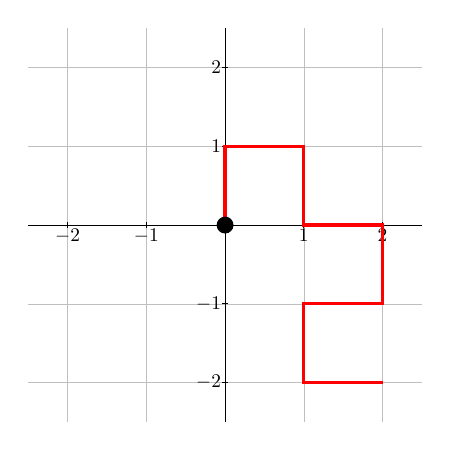
\begin{tikzpicture}
    \draw[step=1, lightgray, very thin] (2.5,2.5) grid (-2.5,-2.5);
    \foreach \i in {-2,-1,1,2}
       \draw (\i, -1pt) -- (\i, 1pt) node[anchor=north, scale=0.7]{$\i$};
    \foreach \i in {-2,-1,1,2}
       \draw (-1pt,\i) -- (1pt,\i) node[anchor=east, scale=0.7]{$\i$};
  \draw[thin] (0,-2.5) -- (0,2.5);
  \draw[thin] (-2.5,0) -- (2.5, 0);
	\draw[very thick,red] (0,0) --(0,1) --(1,1) --(1,0) -- (2,0) --(2,-1) -- (1,-1)--(1,-2) -- (2,-2);
	\draw[fill = black] (0,0) circle (0.1);
	% \end{scope}
	\end{tikzpicture}
\end{center}
\end{minipage}
\\

Diremos que un recorrido del dragón tiene largo $N$ si se ejecuta la acción avanzar $N$ veces.
Por ejemplo, el recorrido descrito anteriormente tiene largo $N = 8$.
Notar que para hacer un recorrido de largo $N$ hay que considerar una secuencia del dragón que tenga al menos $N$ acciones avanzar.
Por ejemplo si se quiere hacer un recorrido de largo $N=5$ hay que considerar la secuencia $ARARRLALARRLARARLLALAR$ y ejecutar
las primeras 5 acciones avanzar.
Esto dejaría a Olon-sonkú en la posición $(2,-1)$.

Supón que Bulnelman sabe que el planeta de Jorgesama se encuentra al final del recorrido del dragón de largo $N$.
?`Puedes ayudarnos a saber cual es la posición exacta del planeta del gran Jorgesama?


\begin{inputDescription}
La entrada consiste en una linea con un único entero positivo $N$.
Tu programa debe calcular las coordenadas del final del recorrido del dragón de largo $N$.
\end{inputDescription}

\begin{outputDescription}
Debes imprimir una única línea con dos enteros $x$ e $y$ separados por un espacio.
Estos enteros corresponden a las coordenadas del planeta del gran Jorgesama.
\end{outputDescription}

\begin{scoreDescription}
\score{10} Se probarán varios casos donde $1 \leq N \leq 8$.
\score{20} Se probarán varios casos donde $1 \leq N \leq 100$.
\score{40} Se probarán varios casos donde $1 \leq N \leq 10^5$.
\score{30} Se probarán varios casos donde $1 \leq N \leq 10^{15}$. 
\\
\\
{\bf Nota:} en la última subtarea el entero $N$ debe ser leído en una variable de tipo long long.
\end{scoreDescription}

\begin{sampleDescription}
\sampleIO{sample1}
\sampleIO{sample2}
\sampleIO{sample3}
\sampleIO{sample4}
\sampleIO{sample5}
\sampleIO{sample6}
\end{sampleDescription}

\end{document}
